% Arquvo LaTeX de exemplo de dissertação/tese a ser apresentada à CPG do IME-USP
%
% Criação: Jesús P. Mena-Chalco
% Revisão: Fabio Kon e Paulo Feofiloff
% Adaptação para UTF8, biblatex e outras melhorias: Nelson Lago
%
% Except where otherwise indicated, these files are distributed under
% the MIT Licence. The example text, which includes the tutorial and
% examples as well as the explanatory comments in the source, are
% available under the Creative Commons Attribution International
% Licence, v4.0 (CC-BY 4.0) - https://creativecommons.org/licenses/by/4.0/


%%%%%%%%%%%%%%%%%%%%%%%%%%%%%%%%%%%%%%%%%%%%%%%%%%%%%%%%%%%%%%%%%%%%%%%%%%%%%%%%
%%%%%%%%%%%%%%%%%%%%%%%%%%%%%%% PREÂMBULO LaTeX %%%%%%%%%%%%%%%%%%%%%%%%%%%%%%%%
%%%%%%%%%%%%%%%%%%%%%%%%%%%%%%%%%%%%%%%%%%%%%%%%%%%%%%%%%%%%%%%%%%%%%%%%%%%%%%%%

% A opção twoside (frente-e-verso) significa que a aparência das páginas pares
% e ímpares pode ser diferente. Por exemplo, as margens podem ser diferentes ou
% os números de página podem aparecer à direita ou à esquerda alternadamente.
% Mas nada impede que você crie um documento "só frente" e, ao imprimir, faça
% a impressão frente-e-verso.
%
% Aqui também definimos a língua padrão do documento
% (a última da lista) e línguas adicionais.
%\documentclass[12pt,twoside,brazilian,english]{book}
\documentclass[12pt,twoside,english]{book}

% Ao invés de definir o tamanho das margens, vamos definir os tamanhos do
% texto, do cabeçalho e do rodapé, e deixamos a package geometry calcular
% o tamanho das margens em função do tamanho do papel. Assim, obtemos o
% mesmo resultado impresso, mas com margens diferentes, se o tamanho do
% papel for diferente.
\usepackage[a4paper]{geometry}

\geometry{
  textwidth=152mm,
  hmarginratio=12:17, % 24:34 -> com papel A4, 24mm + 152mm + 34mm = 210mm
  textheight=237mm,
  vmarginratio=8:7, % 32:28 -> com papel A4, 32mm + 237mm + 28mm = 297mm
  headsep=11mm, % distância entre a base do cabeçalho e o texto
  headheight=21mm, % qualquer medida grande o suficiente, p.ex., top - headsep
  footskip=10mm,
  marginpar=20mm,
  marginparsep=5mm,
}

% Vários pacotes e opções de configuração genéricos; para personalizar o
% resultado, modifique estes arquivos.
%%%%%%%%%%%%%%%%%%%%%%%%%%%%%%%%%%%%%%%%%%%%%%%%%%%%%%%%%%%%%%%%%%%%%%%%%%%%%%%%
%%%%%%%%%%%%%%%%%%%%%%% CONFIGURAÇÕES E PACOTES BÁSICOS %%%%%%%%%%%%%%%%%%%%%%%%
%%%%%%%%%%%%%%%%%%%%%%%%%%%%%%%%%%%%%%%%%%%%%%%%%%%%%%%%%%%%%%%%%%%%%%%%%%%%%%%%

% Vários comandos auxiliares para o desenvolvimento de packages e classes;
% aqui, usamos em alguns comandos de formatação e condicionais.
\usepackage{etoolbox}
%\RequirePackage{pdftexcmds}
\usepackage{letltxmacro}
%\usepackage{ltxcmds}

% LaTeX 3
\usepackage{expl3}
\usepackage{xparse}

% Detecta se estamos usando pdftex, luatex, xetex etc.
\usepackage{iftex}

%\usepackage{xfp} % Floating-point calculations

\usepackage{regexpatch}

% O projeto LaTeX3 renomeou algumas macros em 2019-03-05 e removeu
% a compatibilidade com os nomes antigos em 2020-07-17 a partir de
% 2021-01-01 (veja o arquivo l3deprecation.dtx e o changelog em
% https://github.com/latex3/latex3/blob/main/l3kernel/CHANGELOG.md).
% Isso afetou a package regexpatch: versões antigas da package não
% funcionam com versões novas de LaTeX e vice-versa. Infelizmente,
% ubuntu 21.04 (hirsute) e debian 11 (bullseye) incluem essas versões
% incompatíveis e, portanto, a package regexpatch não funciona nesses
% ambientes. Talvez fosse possível contornar esse problema com a
% package latexrelease, mas isso afetaria muitos outros recursos.
% Ao invés disso, vamos restaurar manualmente a compatibilidade.
% TODO: remover isto após debian bullseye se tornar obsoleta,
%       provavelmente no final de 2024.
\makeatletter
\ExplSyntaxOn

\@ifpackagelater{regexpatch}{2021/03/21}
  {} % Se regexpatch é "nova", expl3 deve ser também; nada a fazer
  {
    % Talvez o correto seja 2021/01/01, mas na prática o resultado é o mesmo
    \@ifpackagelater{expl3}{2020/07/17}
      {
        % As versões são incompatíveis; vamos recuperar as macros preteridas
        \cs_gset:Npn \token_get_prefix_spec:N { \cs_prefix_spec:N }
        \cs_gset:Npn \token_get_arg_spec:N { \cs_argument_spec:N }
        \cs_gset:Npn \token_get_replacement_spec:N { \cs_replacement_spec:N }
      }
      {} % As duas packages são antigas e, portanto, compatíveis entre si
  }
\ExplSyntaxOff
\makeatother

% Algumas packages dependem de xpatch e tentam carregá-la, causando conflitos
% com regexpatch. Como regexpatch oferece todos os recursos de xpatch (ela
% é uma versão estendida de xpatch, mas ainda considerada experimental), vamos
% fazê-las acreditar que xpatch já foi carregada.
\expandafter\xdef\csname ver@xpatch.sty\endcsname{2012/10/02}

% Acrescenta a correção deste bug (contida na release 2018-11-28):
% https://github.com/latex3/latex2e/issues/94 . Se a correção não
% puder ser aplicada, temos uma versão de LaTeX que já a incorpora.
% Esse bug afeta apenas textos em duas colunas.
% TODO: remover após ubuntu 18.04 se tornar obsoleta (abril/2023)
\makeatletter
\patchcmd\@combinedblfloats{\box\@outputbox}{\unvbox\@outputbox}{}{}
\makeatother

% Arithmetic expressions in \set{length,counter} & \addto{length,counter};
% commands \widthof, \heightof, \depthof, \totalheightof, \settototalheight
\usepackage{calc}

% Algumas packages "padrão" da AMS, que são praticamente obrigatórias.
% Algumas delas devem ser carregadas antes de unicode-math ou das
% definições das fontes do documento. É preciso carregar amsthm após
% amsmath para o comando \qedhere funcionar dentro do ambiente align.
\usepackage{amssymb}
\usepackage{amsmath}
\usepackage{amsthm}

% "fontenc" é um parâmetro do NFSS (sistema de gestão de fontes do
% LaTeX; consulte "texdoc fntguide" e "texdoc fontenc"). O default
% é OT1, mas ele tem algumas limitações; a mais importante é que,
% com ele, palavras acentuadas não podem ser hifenizadas. Por
% conta disso, quase todos os documentos LaTeX utilizam o fontenc
% T1. A escolha do fontenc tem consequências para as fontes que
% podem ser usadas com NFSS; hoje em dia T1 tem mais opções de
% qualidade, então não se perde nada em usá-lo. A package fontspec
% (para gestão de fontes usando outro mecanismo, compatível apenas
% com lualatex e xelatex) carrega fontenc automaticamente, mas
% usando outra codificação ("TU" e não "T1"). Ainda assim, é útil
% carregar o fontenc T1 (antes de carregar fontspec!) para o caso
% de alguma fonte "antiga" ser utilizada no documento (embora isso
% não seja recomendado: lualatex e xelatex só são capazes de
% hifenizar palavras acentuadas com o fontenc TU).
\usepackage[T1]{fontenc}

\ifPDFTeX
  % O texto está escrito em utf8.
  \usepackage[utf8]{inputenc}

  % Permitem utilizar small caps + itálico (e outras pequenas
  % melhorias). Em geral, desnecessário com fontspec, a menos
  % que alguma package utilize especificamente. Algumas raras
  % packages de fontes podem causar conflitos com fontaxes, em
  % geral por utilizarem a package "concorrente" nfssext-cfr.
  \usepackage{fontaxes}
  \usepackage{mweights}

  % LaTeX substitui algumas sequências de caracteres, como
  % "fi", "fl" e outras, por caracteres especiais ("ligaduras").
  % Para que seja possível fazer copiar/colar ou buscas por
  % textos contendo essas ligaduras, o arquivo PDF precisa
  % conter uma tabela indicando quais são elas. Com fontes
  % OTF (LuaLaTeX ou XeLaTeX) isso não costuma ser um problema,
  % mas com pdfLaTeX pode ser. Estes dois comandos (que só
  % existem no pdfLaTeX) incluem uma tabela genérica que
  % funciona para a maioria das fontes. Veja a seção 5 de
  % http://www.tug.org/TUGboat/Articles/tb29-1/tb91thanh-fonts.pdf
  % Note que alguns visualizadores de PDF tentam "adivinhar"
  % o conteúdo da tabela quando ela está incompleta ou não
  % existe, então copiar/colar e buscas podem funcionar em
  % alguns visualizadores e em outros não.
  \input glyphtounicode.tex
  \pdfgentounicode=1
\else
  % Não é preciso carregar inputenc com LuaTeX e XeTeX, pois
  % com eles utf8 é obrigatório.
  \usepackage{fontspec}

  % Ao invés de usar o sistema tradicional de LaTeX para gerir
  % as fontes matemáticas, utiliza as extensões matemáticas do
  % formato otf definidas pela microsoft. Ao ativar esta package
  % o mecanismo tradicional não funciona mais! Há poucas fontes
  % com suporte a unicode-math.
  \usepackage{unicode-math}
\fi

% Acesso a símbolos adicionais, como \textrightarrow, \texteuro etc.,
% disponíveis na maioria das fontes através do fontenc TS1 ou mudando
% momentaneamente para computer modern/latin modern. Raramente útil
% com lualatex/xelatex, mas não causa problemas. Várias packages de
% fontes carregam textcomp, às vezes com opções específicas; assim,
% para evitar problemas, vamos carregá-la no final do preâmbulo para
% o caso de ela não ter sido carregada antes.
\AtBeginDocument{\usepackage{textcomp}}

% TeXLive 2018 inclui a versão 2.7a da package microtype e a versão
% 1.07 de luatex. Essa combinação faz aparecer um bug:
% https://tex.stackexchange.com/a/476742
% Aqui, aplicamos a solução sugerida, que não tem "contra-indicações".
\ifLuaTeX
  \usepackage{luatexbase}
\fi

% microajustes no tamanho das letras, espaçamento etc. para melhorar
% a qualidade visual do resultado.
\usepackage{microtype}

% Alguns "truques" (sujos?) para minimizar over/underfull boxes.
%
% Para fazer um texto justificado, é preciso modificar o tamanho dos espaços
% em cada linha para mais ou para menos em relação ao seu tamanho ideal. Para
% escolher as quebras de linha, TeX vai percorrendo o texto procurando lugares
% possíveis para quebrar as linhas considerando essa flexibilidade mas dentro
% de um certo limite mínimo/máximo. Nesse processo, ele associa a cada possível
% linha o valor *badness*, que é o nível de distorção do tamanho dos espaços
% daquela linha em relação ao ideal, e ignora opções que tenham badness muito
% grande (esse limite é dado por \tolerance). Depois de encontradas todas
% as possíveis quebras de linha e a badness de cada uma, TeX calcula as
% *penalties* das quebras encontradas, que são uma medida de quebras "ruins".
% Por exemplo, na configuração padrão, quebrar uma linha hifenizando uma
% palavra gera uma penalty de 50; já uma quebra que faça a última linha
% do parágrafo ficar sozinha na página seguinte gera uma penalty de 150.
% Finalmente, TeX calcula a "feiúra" de cada possível linha (demerits)
% com base na badness e nas penalties e escolhe a solução que minimiza os
% demerits totais do parágrafo. Os comandos \linebreak e \pagebreak funcionam
% simplesmente acrescentando uma penalty negativa ao lugar desejado para a
% quebra.
%
% Para cada fonte, o espaço entre palavras tem um tamanho ideal, um
% tamanho mínimo e um tamanho máximo (é possível obter os valores com
% \number\fontdimenX\font\relax, veja https://tex.stackexchange.com/q/88991 ).
% TeX nunca reduz um espaço para menos que o mínimo da fonte, mas pode
% aumentá-lo para mais que o máximo. Se os espaços de uma linha ficam
% com o tamanho ideal, a badness da linha é 0; se o tamanho é
% reduzido/aumentado 50% do mínimo/máximo, a badness da linha é 12; se
% o tamanho é reduzido/aumentado para o mínimo/máximo, a badness é 100,
% e assim por diante. O valor máximo possível para badness é 10.000, que
% significa "badness infinita". Como é feito o cálculo: se as medidas
% do espaço definidas pela fonte são "x plus y minus z" e o tamanho
% final do espaço é "x + k*y" ou "x - k*z", a badness é 100*(k^3). Com
% Libertinus corpo 12, os valores são "3pt plus 1.5pt minus .9996pt",
% Então se o espaço tiver sido aumentado para 3.75pt, o fator é 0.5 e
% a badness é 100*(.5^3) = 12.
%
% \tolerance indica a badness máxima que TeX aceita para uma linha; seu valor
% default é 200. Assim, aumentar para, digamos, 300 ou 400, permite que
% TeX escolha parágrafos com maior variação no espaçamento entre as palavras.
% No entanto, no cálculo de demerits, a badness e as penalties de cada linha
% são elevadas ao quadrado, então TeX geralmente prefere escolher outras
% opções no lugar de uma linha com espaçamento ruim. Por exemplo, órfãs/viúvas
% têm demerit de 22.500 e dois hífens seguidos têm demerit de 10.000; já uma
% linha com badness 400 tem demerit 160.000. Portanto, não é surpreendente que
% a maioria dos parágrafos tenha demerits abaixo de 40.000, quase todos abaixo
% de 100.000 e praticamente nenhum acima de 1.000.000. Isso significa que, para
% a grande maioria dos parágrafos, aumentar \tolerance não faz diferença: uma
% linha com badness 400 nunca será efetivamente escolhida se houver qualquer
% outra opção com badness menor. Também fica claro que não há muita diferença
% real entre definir \tolerance como 800 ou 9.999 (a não ser fazer TeX
% trabalhar mais desnecessariamente).
%
% O problema muda de figura se TeX não consegue encontrar uma solução. Isso
% pode acontecer em dois casos: (1) o parágrafo tem ao menos uma linha que não
% pode ser quebrada com badness < 10.000 ou (2) o parágrafo tem ao menos uma
% linha que não pode ser quebrada com badness < tolerance (mas essa badness é
% menor que 10.000).
%
% No primeiro caso, se houver várias possibilidades de linhas que não podem ser
% quebradas, TeX não vai ser capaz de compará-las e escolher a melhor: todas
% têm a badness máxima (10.000) e, portanto, a que gerar menos deméritos no
% restante do parágrafo será a escolhida. Na realidade, no entanto, essas
% linhas *não* são igualmente ruins entre si, o que pode levar TeX a fazer uma
% má escolha. Para evitar isso, TeX tenta novamente aplicando
% \emergencystretch, que "faz de conta" que o tamanho máximo ideal dos espaços
% da linha é maior que o definido na fonte. Isso reduz a badness de todas as
% linhas, o que soa parecido com aumentar \tolerance. Há três diferenças, no
% entanto: (1) essa mudança só afeta os parágrafos que falharam; (2) soluções
% que originalmente teriam badness = 10.000 (e, portanto, seriam vistas como
% equivalentes) podem ser avaliadas e comparadas entre si; e (3) como a badness
% de todas as linhas diminui, a possibilidade de outras linhas que
% originalmente tinham badness alta serem escolhidas aumenta. Esse último ponto
% significa que \emergencystretch pode fazer TeX escolher linhas mais
% espaçadas, fazendo o espaçamento do parágrafo inteiro aumentar e, portanto,
% tornando o resultado mais homogêneo mesmo com uma linha particularmente ruim.
%
% É esse último ponto que justifica o uso de \emergencystretch no segundo caso
% também: apenas aumentar a tolerância, nesse caso, poderia levar TeX a
% diagramar uma linha ruim em meio a um parágrafo bom, enquanto
% \emergencystretch pode fazer TeX aumentar o espaçamento de maneira geral no
% parágrafo, minimizando o contraste da linha problemática com as demais.
% Colocando a questão de outra maneira, aumentar \tolerance para lidar com
% esses parágrafos problemáticos pode fazê-los ter uma linha especialmente
% ruim, enquanto \emergencystretch pode dividir o erro entre várias linhas.
% Assim, definir \tolerance em torno de 800 parece razoável: no caso geral,
% não há diferença e, se um desses casos difíceis não pode ser resolvido com
% uma linha de badness até 800, \emergencystretch deve ser capaz de gerar um
% resultado igual ou melhor.
%
% Penalties & demerits: https://tex.stackexchange.com/a/51264
% Definições (fussy, sloppy etc.): https://tex.stackexchange.com/a/241355
% Mais definições (hfuzz, hbadness etc.): https://tex.stackexchange.com/a/50850
% Donald Arseneau defendendo o uso de \sloppy: https://groups.google.com/d/msg/comp.text.tex/Dhf0xxuQ66E/QTZ7aLYrdQUJ
% Artigo detalhado sobre \emergencystretch: https://www.tug.org/TUGboat/tb38-1/tb118wermuth.pdf
% Esse artigo me leva a crer que algo em torno de 1.5em é suficiente

\tolerance=800
\hyphenpenalty=100 % Default 50; se o texto é em 2 colunas, 50 é melhor
\setlength{\emergencystretch}{1.5em}

% Não gera warnings para Overfull menor que 1pt
\hfuzz=1pt
\vfuzz\hfuzz

% Não gera warnings para Underfull com badness < 1000
\hbadness=1000
\vbadness=1000

% Por padrão, o algoritmo LaTeX para textos não-justificados é (muito) ruim;
% este pacote implementa um algoritmo bem melhor
\usepackage[newcommands]{ragged2e}

% ragged2e funciona porque permite que LaTeX hifenize palavras em textos
% não-justificados quando necessário. No caso de textos centralizados,
% no entanto, isso em geral não é desejável. Assim, newcommands não é
% interessante para \centering e \begin{center}. newcommands também
% causa problemas com legendas se o float correspondente usa \centering
% (o que é muito comum). Assim, vamos voltar \centering e \begin{center}
% à definição padrão.
\let\centering\LaTeXcentering
\let\center\LaTeXcenter
\let\endcenter\endLaTeXcenter

% Com ragged2e e a opção "newcommands", textos curtos não-justificados
% podem gerar warnings sobre "underfull \hbox". Não há razão para pensar
% muito nesses warnings, então melhor desabilitá-los.
% https://tex.stackexchange.com/a/18019
\makeatletter
\gappto{\raggedright}{\hbadness=\@M}
\gappto{\RaggedRight}{\hbadness=\@M}
\gappto{\raggedleft}{\hbadness=\@M}
\gappto{\RaggedLeft}{\hbadness=\@M}
\gappto{\Centering}{\hbadness=\@M} % not \centering
\gappto{\flushleft}{\hbadness=\@M}
\gappto{\FlushLeft}{\hbadness=\@M}
\gappto{\flushright}{\hbadness=\@M}
\gappto{\FlushRight}{\hbadness=\@M}
\gappto{\Center}{\hbadness=\@M} % not \center
\makeatother

% Espaçamento entre linhas configurável (\singlespacing, \onehalfspacing etc.)
\usepackage{setspace}

% LaTeX às vezes coloca notas de rodapé logo após o final do texto da
% página ao invés de no final da página; este pacote evita isso e faz
% notas de rodapé funcionarem corretamente em títulos de seções.
% Esta package deve ser carregada depois de setspace.
\usepackage[stable,bottom]{footmisc}

% Se uma página está vazia, não imprime número de página ou cabeçalho
\usepackage{emptypage}

% hyperref deve preferencialmente ser carregada próximo ao final
% do preâmbulo mas, para o caso de alguma package forçar a sua
% carga antes de executarmos \usepackage explicitamente, vamos
% garantir que estas opções estejam ativas.
\PassOptionsToPackage{
  unicode=true,
  pdfencoding=unicode,
  plainpages=false,
  pdfpagelabels,
  bookmarksopen=true,
  breaklinks=true,
  %hyperfootnotes=false, % polui desnecessariamente com bordercolor
}{hyperref}

% Carrega nomes de cores disponíveis (podem ser usados com hyperref e listings)
\usepackage[hyperref,svgnames,x11names,table]{xcolor}

% LaTeX define os comandos "MakeUppercase" e "MakeLowercase", mas eles têm
% algumas limitações; esta package define os comandos MakeTextUppercase e
% MakeTextLowercase que resolvem isso.
\usepackage{textcase}

% Em documentos frente-e-verso, LaTeX faz o final da página terminar sempre
% no mesmo lugar (exceto no final dos capítulos). Esse comportamento pode ser
% ativado explicitamente com o comando "\flushbottom". Mas se, por alguma
% razão, o volume de texto na página é "pequeno", essa página vai ter espaços
% verticais artificialmente grandes. Uma solução para esse problema é utilizar
% "\raggedbottom" (padrão em documentos que não são frente-e-verso): com essa
% opção, as páginas podem terminar em alturas ligeiramente diferentes. Outra
% opção é corrigir manualmente cada página problemática, por exemplo com o
% comando "\enlargethispage".
%\raggedbottom
\flushbottom

% Por padrão, LaTeX coloca uma espaço aumentado após sinais de pontuação;
% Isso não é tão bom quanto alguns TeX-eiros defendem :) .
% Esta opção desabilita isso e, consequentemente, evita problemas com
% "id est" (i.e.) e "exempli gratia" (e.g.)
\frenchspacing

% Trechos de texto "puro" (tabs, quebras de linha etc. não são modificados)
\usepackage{verbatim}

% Durante o processamento, LaTeX procura por arquivos adicionais necessários
% (tanto componentes do próprio LaTeX, como packages e fontes, quanto partes
% do conteúdo em si, como imagens carregadas com \includegraphics ou arquivos
% solicitados com \input ou \include) no diretório de instalação e também
% no diretório atual (ou seja, o diretório do projeto). Assim, normalmente
% é preciso usar caminhos relativos para incluir arquivos de subdiretórios:
% "\input{diretorio/arquivo}". No entanto, há duas limitações:
%
% 1. É necessário dizer "\input{diretorio/arquivo}" mesmo quando o arquivo
%    que contém esse comando já está dentro do subdiretório.
%
% 2. Isso não deve ser usado para packages ("\usepackage{diretorio/package}"),
%    embora na prática funcione.
%
% Há três maneiras recomendadas de resolver esses problemas:
%
% 1. Acrescentando os diretórios desejados ao arquivo texmf.cnf
%
% 2. Acrescentando os diretórios desejados às variáveis de ambiente
%    TEXINPUTS e BSTINPUTS
%
% 3. Colocando os arquivos adicionais na árvore TEXMF (geralmente, no
%    diretório texmf dentro do diretório do usuário).
%
% Essas soluções, no entanto, não podem ser automatizadas por este modelo
% e são um tanto complicadas para usuários menos experientes. Veja mais a
% respeito na seção 5 de "texdoc kpathsea" e em
% https://www.overleaf.com/learn/latex/Articles/An_introduction_to_Kpathsea_and_how_TeX_engines_search_for_files .
%
% A package import pode solucionar o primeiro problema, mas exige o uso
% de outro comando no lugar de \input, então não a usamos aqui.
%\usepackage{import}
%
% Uma solução mais simples é acrescentar os diretórios desejados à macro
% \input@path, originalmente criada para resolver um problema relacionado
% à portabilidade. Seu uso não é normalmente recomendado por razões de
% desempenho, mas no nosso caso (em que adicionamos apenas um diretório
% com poucos arquivos e com máquinas modernas) isso não é um problema. Veja
% https://tex.stackexchange.com/questions/241828/define-path-for-packages-in-the-latex-file-analog-of-inputpath-or-graphicspa#comment705011_241832
\csappto{input@path}{{extras/}}

%%%%%%%%%%%%%%%%%%%%%%%%%%%%%%%%%%%%%%%%%%%%%%%%%%%%%%%%%%%%%%%%%%%%%%%%%%%%%%%%
%%%%%%%%%%%%%%%%%%%%%%%%%%%%%%%%%%% LÍNGUAS %%%%%%%%%%%%%%%%%%%%%%%%%%%%%%%%%%%%
%%%%%%%%%%%%%%%%%%%%%%%%%%%%%%%%%%%%%%%%%%%%%%%%%%%%%%%%%%%%%%%%%%%%%%%%%%%%%%%%

\makeatletter
\ExplSyntaxOn

% We need to have at least some variant of Portuguese and of English
% loaded to generate the abstract/resumo, palavras-chave/keywords etc.
% We will make sure that both languages are present in the class options
% list by adding them if needed. With this, these options become global
% and therefore are seen by all packages (among them, babel).
%
% babel traditionally uses "portuguese", "brazilian", "portuges", or
% "brazil" to support the Portuguese language, using .ldf files. babel
% is also in the process of implementing a new scheme, using .ini
% files, based on the concept of "locales" instead of "languages". This
% mechanism uses the names "portuguese-portugal", "portuguese-brazil",
% "portuguese-pt", "portuguese-br", "portuguese", "brazilian", "pt",
% "pt-PT", and "pt-BR" (i.e., neither "portuges" nor "brazil"). To avoid
% compatibility problems, let's stick with "brazilian" or "portuguese"
% by substituting portuges and brazil if necessary.

\NewDocumentCommand\@IMEportugueseAndEnglish{m}{

  % Make sure any instances of "portuges" and "brazil" are replaced
  % by "portuguese" e "brazilian"; other options are unchanged.
  \seq_gclear_new:N \l_tmpa_seq
  \seq_gclear_new:N \l_tmpb_seq
  \seq_gset_from_clist:Nc \l_tmpa_seq {#1}

  \seq_map_inline:Nn \l_tmpa_seq{
    \def\@tempa{##1}
    \ifstrequal{portuges}{##1}
      {
        \GenericInfo{sbc2019}{}{Substituting~language~portuges~->~portuguese}
        \def\@tempa{portuguese}
      }
      {}
    \ifstrequal{brazil}{##1}
      {
        \GenericInfo{}{Substituting~language~brazil~->~brazilian}
        \def\@tempa{brazilian}
      }
      {}
    \seq_gput_right:NV \l_tmpb_seq {\@tempa}
  }

  % Remove the leftmost duplicates (default is to remove the rightmost ones).
  % Necessary in case the user did "portuges,portuguese", "brazil,brazilian"
  % or some variation: When we substitute the language, we end up with the
  % exact same language twice, which may mess up the main language selection.
  \seq_greverse:N \l_tmpb_seq
  \seq_gremove_duplicates:N \l_tmpb_seq
  \seq_greverse:N \l_tmpb_seq

  % If the user failed to select some variation of English and Portuguese,
  % we add them here. We also remember which ones of portuguese/brazilian,
  % english/american/british etc. were selected.
  \exp_args:Nnx \regex_extract_all:nnNTF
    {\b(portuguese|brazilian)\b}
    {\seq_use:Nn \l_tmpb_seq {,}}
    \l_tmpa_tl
    {
      \tl_reverse:N \l_tmpa_tl
      \xdef\@IMEpt{\tl_head:N \l_tmpa_tl}
    }
    {
      \seq_gput_left:Nn \l_tmpb_seq {brazilian}
      \gdef\@IMEpt{brazilian}
    }

  \exp_args:Nnx \regex_extract_all:nnNTF
    {\b(english|american|USenglish|canadian|british|UKenglish|australian|newzealand)\b}
    {\seq_use:Nn \l_tmpb_seq {,}}
    \l_tmpa_tl
    {
      \tl_reverse:N \l_tmpa_tl
      \xdef\@IMEen{\tl_head:N \l_tmpa_tl}
    }
    {
      \seq_gput_left:Nn \l_tmpb_seq {english}
      \gdef\@IMEen{english}
    }

  \exp_args:Nc \xdef {#1} {\seq_use:Nn \l_tmpb_seq {,}}
}


% https://tex.stackexchange.com/a/43541
% This message is part of a larger thread that discusses some
% limitations of this method, but it is enough for us here.
\def\@getcl@ss#1.cls#2\relax{\def\@currentclass{#1}}
\def\@getclass{\expandafter\@getcl@ss\@filelist\relax}
\@getclass

% The three class option lists we need to update: \@unusedoptionlist,
% \@classoptionslist and one of \opt@book.cls, \opt@article.cls etc.
% according to the current class. Note that beamer.cls (and maybe
% others) does not use \@unusedoptionlist; with it, we incorrectly
% add "english,brazilian" to \@unusedoptionlist, but that does not
% cause problems.
\@IMEportugueseAndEnglish{@unusedoptionlist}
\@IMEportugueseAndEnglish{@classoptionslist}
\@IMEportugueseAndEnglish{opt@\@currentclass .cls}

\ExplSyntaxOff
\makeatother

% Internacionalização dos nomes das seções ("chapter" X "capítulo" etc.),
% hifenização e outras convenções tipográficas. babel deve ser um dos
% primeiros pacotes carregados. É possível passar a língua do documento
% como parâmetro aqui, mas já fizemos isso ao carregar a classe, no início
% do documento.
\usepackage{babel}
\usepackage{iflang}

% É possível personalizar as palavras-chave que babel utiliza, por exemplo:
%\addto\extrasbrazilian{\renewcommand{\chaptername}{Chap.}}
% Com BibTeX, isso vale também para a bibliografia; com BibLaTeX, é melhor
% usar o comando "DefineBibliographyStrings".

% Para línguas baseadas no alfabeto latino, como o inglês e o português,
% o pacote babel funciona muito bem, mas com outros alfabetos ele às vezes
% falha. Por conta disso, o pacote polyglossia foi criado para substituí-lo.
% polyglossia só funciona com LuaTeX e XeTeX; como babel também funciona com
% esses sistemas, provavelmente não há razão para usar polyglossia, mas é
% possível que no futuro esse pacote se torne o padrão.
%\usepackage{polyglossia}
%\setdefaultlanguage{brazilian}
%\setotherlanguage{english}

% Alguns pacotes (espeficicamente, tikz) usam, além de babel, este pacote
% como auxiliar para a tradução de palavras-chave, como os meses do ano.
\usepackage{translator}

%%%%%%%%%%%%%%%%%%%%%%%%%%%%%%%%%%%%%%%%%%%%%%%%%%%%%%%%%%%%%%%%%%%%%%%%%%%%%%%%
%%%%%%%%%%%%%%%%%%%%%%%%%%%%%%%%%%% FONTE %%%%%%%%%%%%%%%%%%%%%%%%%%%%%%%%%%%%%%
%%%%%%%%%%%%%%%%%%%%%%%%%%%%%%%%%%%%%%%%%%%%%%%%%%%%%%%%%%%%%%%%%%%%%%%%%%%%%%%%

% LaTeX normalmente usa quatro tipos de fonte:
%
% * uma fonte serifada, para o corpo do texto;
% * uma fonte com design similar à anterior, para modo matemático;
% * uma fonte sem serifa, para títulos ou "entidades". Por exemplo, "a classe
%   \textsf{TimeManager} é responsável..." ou "chamamos \textsf{primos} os
%   números que...". Observe que em quase todos os casos desse tipo é mais
%   adequado usar negrito ou itálico;
% * uma fonte "teletype", para trechos de programas.
%
% A escolha de uma família de fontes para o documento normalmente é feita
% carregando uma package específica que, em geral, seleciona as quatro fontes
% de uma vez.
%
% LaTeX usa por default a família de fontes "Computer Modern". Essas fontes
% precisaram ser re-criadas diversas vezes em formatos diferentes, então há
% diversas variantes dela. Com o fontenc OT1 (default "ruim" do LaTeX), a
% versão usada é a BlueSky Computer Modern, que é de boa qualidade, mas com
% os problemas do OT1. Com fontenc T1 (padrão deste modelo e recomendado), o
% LaTeX usa o conjunto "cm-super". Com fontspec (ou seja, com LuaLaTeX e
% XeLaTeX), LaTeX utiliza a versão "Latin Modern". Ao longo do tempo, versões
% diferentes dessas fontes foram recomendadas como "a melhor"; atualmente, a
% melhor opção para usar a família Computer Modern é a versão "Latin Modern".
%
% Você normalmente não precisa lidar com isso, mas pode ser útil saber: O
% mecanismo tradicionalmente usado por LaTeX para gerir fontes é o NFSS
% (veja "texdoc fntguide"). Ele funciona com todas as versões de LaTeX,
% mas só com fontes que foram adaptadas para funcionar com LaTeX. LuaLaTeX
% e XeLaTeX podem usar NFSS mas também são capazes de utilizar um outro
% mecanismo (através da package fontspec), que permite utilizar quaisquer
% fontes instaladas no computador.

\ifPDFTeX
    % Usando pdfLaTeX

    % Ativa Latin Modern como a fonte padrão.
    \usepackage{lmodern}

    % Alguns truques para melhorar a aparência das fontes Latin Modern;
    % eles não funcionam com LuaLaTeX e XeLaTeX.

    % Latin Modern não tem fontes bold + Small Caps, mas cm-super sim;
    % assim, vamos ativar o suporte às fontes cm-super (sem ativá-las
    % como a fonte padrão do documento) e configurar substituições
    % automáticas para que a fonte Latin Modern seja substituída por
    % cm-super quando o texto for bold + Small Caps.
    \usepackage{fix-cm}

    % Com Latin Modern, é preciso incluir substituições para o encoding TS1
    % também por conta dos números oldstyle, porque para inclui-los nas fontes
    % computer modern foi feita uma hack: os dígitos são declarados como sendo
    % os números itálicos da fonte matemática e, portanto, estão no encoding TS1.
    %
    % Primeiro forçamos o LaTeX a carregar a fonte Latin Modern (ou seja, ler
    % o arquivo que inclui "DeclareFontFamily") e, a seguir, definimos a
    % substituição
    \fontencoding{TS1}\fontfamily{lmr}\selectfont
    \DeclareFontShape{TS1}{lmr}{b}{sc}{<->ssub * cmr/bx/n}{}
    \DeclareFontShape{TS1}{lmr}{bx}{sc}{<->ssub * cmr/bx/n}{}

    \fontencoding{T1}\fontfamily{lmr}\selectfont
    \DeclareFontShape{T1}{lmr}{b}{sc}{<->ssub * cmr/bx/sc}{}
    \DeclareFontShape{T1}{lmr}{bx}{sc}{<->ssub * cmr/bx/sc}{}

    % Latin Modern não tem "small caps + itálico", mas tem "small caps + slanted";
    % vamos definir mais uma substituição aqui.
    \fontencoding{T1}\fontfamily{lmr}\selectfont % já feito acima, mas tudo bem
    \DeclareFontShape{T1}{lmr}{m}{scit}{<->ssub * lmr/m/scsl}{}
    \DeclareFontShape{T1}{lmr}{bx}{scit}{<->ssub * lmr/bx/scsl}{}

    % Se fizermos mudanças manuais na fonte Latin Modern, estes comandos podem
    % vir a ser úteis
    %\newcommand\lmodern{%
    %  \renewcommand{\oldstylenums}[1]{{\fontencoding{TS1}\selectfont ##1}}%
    %  \fontfamily{lmr}\selectfont%
    %}
    %
    %\DeclareRobustCommand\textlmodern[1]{%
    %  {\lmodern #1}%
    %}
\else
    % Com LuaLaTex e XeLaTeX, Latin Modern é a fonte padrão. Existem
    % diversas packages e "truques" para melhorar alguns aspectos de
    % Latin Modern, mas eles foram feitos para pdflatex (veja o "else"
    % logo abaixo). Assim, se você pretende usar Latin Modern como a
    % fonte padrão do documento, é melhor usar pdfLaTeX. Deve ser
    % possível implementar essas melhorias com fontspec também, mas
    % este modelo não faz isso, apenas ativamos Small Caps aqui.

    \ifLuaTeX
      % Com LuaTeX, basta indicar o nome de cada fonte; para descobrir
      % o nome "certo", use o comando "otfinfo -i" e veja os itens
      % "preferred family" e "full name"
      \setmainfont{Latin Modern Roman}[
        SmallCapsFont = {LMRomanCaps10-Regular},
        ItalicFeatures = {
          SmallCapsFont = {LMRomanCaps10-Oblique},
        },
        SlantedFont = {LMRomanSlant10-Regular},
        SlantedFeatures = {
          SmallCapsFont = {LMRomanCaps10-Oblique},
          BoldFont = {LMRomanSlant10-Bold}
        },
      ]
    \fi

    \ifXeTeX
      % Com XeTeX, é preciso informar o nome do arquivo de cada fonte.
      \setmainfont{lmroman10-regular.otf}[
        SmallCapsFont = {lmromancaps10-regular.otf},
        ItalicFeatures = {
          SmallCapsFont = {lmromancaps10-oblique.otf},
        },
        SlantedFont = {lmromanslant10-regular.otf},
        SlantedFeatures = {
          SmallCapsFont = {lmromancaps10-oblique.otf},
          BoldFont = {lmromanslant10-bold.otf}
        },
      ]
    \fi
\fi

% Algumas packages mais novas que tratam de fontes funcionam corretamente
% tanto com fontspec (LuaLaTeX/XeLaTeX) quanto com NFSS (qualquer versão
% de LaTeX, mas menos poderoso que fontspec). No entanto, muitas funcionam
% apenas com NFSS. Nesse caso, em LuaLaTeX/XeLaTeX é melhor usar os
% comandos de fontspec, como exemplificado mais abaixo.

% É possível mudar apenas uma das fontes. Em particular, a fonte
% teletype da família Computer Modern foi criada para simular
% as impressoras dos anos 1970/1980. Sendo assim, ela é uma fonte (1)
% com serifas e (2) de espaçamento fixo. Hoje em dia, é mais comum usar
% fontes sem serifa para representar código-fonte. Além disso, ao imprimir,
% é comum adotar fontes que não são de espaçamento fixo para fazer caber
% mais caracteres em uma linha de texto. Algumas opções de fontes para
% esse fim:
%\usepackage{newtxtt} % Não funciona com fontspec (lualatex / xelatex)
%\usepackage{DejaVuSansMono}
% inconsolata é uma boa fonte, mas não tem variante itálico
%\ifPDFTeX
%  \usepackage[narrow]{inconsolata}
%\else
%  \setmonofont{inconsolatan}
%\fi
\usepackage[scale=.85]{sourcecodepro}

% Ao invés da família Computer Modern, é possível usar outras como padrão.
% Uma ótima opção é a libertine, similar (mas não igual) à Times mas com
% suporte a Small Caps e outras qualidades. A fonte teletype da família
% é serifada, então é melhor definir outra; a opção "mono=false" faz
% o pacote não carregar sua própria fonte, mantendo a escolha anterior.
% Versões mais novas de LaTeX oferecem um fork desta fonte, libertinus.
% As packages libertine/libertinus funcionam corretamente com pdfLaTeX,
% LuaLaTeX e XeLaTeX.
% TODO: remover suporte a Libertine no final de 2022
\makeatletter
\IfFileExists{libertinus.sty}
    {
      \usepackage[mono=false]{libertinus}
      % Com LuaLaTeX/XeLaTeX, Libertinus configura também
      % a fonte matemática; aqui só precisamos corrigir \mathit
      \ifLuaTeX
        \setmathfontface\mathit{Libertinus Serif Italic}
      \fi
      \ifXeTeX
        % O nome de arquivo da fonte mudou na versão 2019-04-04
        \@ifpackagelater{libertinus-otf}{2019/04/03}
            {\setmathfontface\mathit{LibertinusSerif-Italic.otf}}
            {\setmathfontface\mathit{libertinusserif-italic.otf}}
      \fi
    }
    {
      % Libertinus não está disponível; vamos usar libertine
      \usepackage[mono=false]{libertine}

      % Com Libertine, é preciso modificar também a fonte
      % matemática, além de \mathit
      \ifLuaTeX
        \setmathfont{Libertinus Math}
        \setmathfontface\mathit{Linux Libertine O Italic}
      \fi

      \ifXeTeX
        \setmathfont{libertinusmath-regular.otf}
        \setmathfontface\mathit{LinLibertine_RI.otf}
      \fi
    }
\makeatother

\ifPDFTeX
  % A família libertine por padrão não define uma fonte matemática
  % específica para pdfLaTeX; uma opção que funciona bem com ela:
  %\usepackage[libertine]{newtxmath}
  % Outra, provavelmente melhor:
  \usepackage{libertinust1math}
\fi

% Ativa apenas a fonte biolinum, que é a fonte sem serifa da família.
%\IfFileExists{libertinus.sty}
%  \usepackage[sans]{libertinus}
%\else
%  \usepackage{biolinum}
%\fi

% Também é possível usar a Times como padrão; nesse caso, a fonte
% sem serifa usualmente é a Helvetica. Mas provavelmente libertine
% é uma opção melhor.
%\ifPDFTeX
%  \usepackage[helvratio=0.95,largesc]{newtxtext}
%  \usepackage{newtxtt} % Fonte teletype
%  \usepackage{newtxmath}
%\else
%  % Clone da fonte Times como fonte principal
%  \setmainfont{TeX Gyre Termes}
%  \setmathfont[Scale=MatchLowercase]{TeX Gyre Termes Math}
%  % TeX Gyre Termes Math tem um bug e não define o caracter
%  % \setminus; Vamos contornar esse problema usando apenas
%  % esse caracter da fonte STIX Two Math
%  \setmathfont[range=\setminus]{STIX Two Math}
%  % Clone da fonte Helvetica como fonte sem serifa
%  \setsansfont{TeX Gyre Heros}
%  % Clone da Courier como fonte teletype, mas provavelmente
%  % é melhor utilizar sourcecodepro
%  %\setmonofont{TeX Gyre Cursor}
%\fi

% Cochineal é outra opção de qualidade; ela define apenas a fonte
% com serifa.
%
% Com NFSS (recomendado no caso de cochineal):
%\usepackage{cochineal}
%\usepackage[cochineal,vvarbb]{newtxmath}
%\usepackage[cal=boondoxo]{mathalfa}
%
% Com fontspec (até a linha "setmathfontface..."):
%
%\setmainfont{Cochineal}[
%  Extension=.otf,
%  UprightFont=*-Roman,
%  ItalicFont=*-Italic,
%  BoldFont=*-Bold,
%  BoldItalicFont=*-BoldItalic,
%  %Numbers={Proportional,OldStyle},
%]
%
%\DeclareRobustCommand{\lfstyle}{\addfontfeatures{Numbers=Lining}}
%\DeclareTextFontCommand{\textlf}{\lfstyle}
%\DeclareRobustCommand{\tlfstyle}{\addfontfeatures{Numbers={Tabular,Lining}}}
%\DeclareTextFontCommand{\texttlf}{\tlfstyle}
%
%% Cochineal não tem uma fonte matemática; com fontspec, provavelmente
%% o melhor a fazer é usar libertinus.
%\setmathfont{Libertinus Math}
%\setmathfontface\mathit{Cochineal-Italic.otf}

% gentium inclui apenas uma fonte serifada, similar a Garamond, que busca
% cobrir todos os caracteres unicode
%\usepackage{gentium}

% LaTeX normalmente funciona com fontes que foram adaptadas para ele, ou
% seja, ele não usa as fontes padrão instaladas no sistema: para usar
% uma fonte é preciso ativar o pacote correspondente, como visto acima.
% É possível escapar dessa limitação e acessar as fontes padrão do sistema
% com XeTeX ou LuaTeX. Com eles, além dos pacotes de fontes "tradicionais",
% pode-se usar o pacote fontspec para usar fontes do sistema.
%\usepackage{fontspec}
%\setmainfont{DejaVu Serif}
%\setmainfont{Charis SIL}
%\setsansfont{DejaVu Sans}
%\setsansfont{Libertinus Sans}[Scale=1.1]
%\setmonofont{DejaVu Sans Mono}

% fontspec oferece vários recursos interessantes para manipular fontes.
% Por exemplo, Garamond é uma fonte clássica; a versão EBGaramond é muito
% boa, mas não possui versões bold e bold-italic; aqui, usamos
% CormorantGaramond ou Gentium para simular a versão bold.
%\setmainfont{EBGaramond12}[
%  Numbers        = {Lining,} ,
%  Scale          = MatchLowercase ,
%  UprightFont    = *-Regular ,
%  ItalicFont     = *-Italic ,
%  BoldFont       = gentiumbasic-bold ,
%  BoldItalicFont = gentiumbasic-bolditalic ,
%%  BoldFont       = CormorantGaramond Bold ,
%%  BoldItalicFont = CormorantGaramond Bold Italic ,
%]
%
%\newfontfamily\garamond{EBGaramond12}[
%  Numbers        = {Lining,} ,
%  Scale          = MatchLowercase ,
%  UprightFont    = *-Regular ,
%  ItalicFont     = *-Italic ,
%  BoldFont       = gentiumbasic-bold ,
%  BoldItalicFont = gentiumbasic-bolditalic ,
%%  BoldFont       = CormorantGaramond Bold ,
%%  BoldItalicFont = CormorantGaramond Bold Italic ,
%]

% Crimson tem Small Caps, mas o recurso é considerado "em construção".
% Vamos utilizar Gentium para Small Caps
%\setmainfont{Crimson}[
%  Numbers           = {Lining,} ,
%  Scale             = MatchLowercase ,
%  UprightFont       = *-Roman ,
%  ItalicFont        = *-Italic ,
%  BoldFont          = *-Bold ,
%  BoldItalicFont    = *-Bold Italic ,
%  SmallCapsFont     = Gentium Plus ,
%  SmallCapsFeatures = {Letters=SmallCaps} ,
%]
%
%\newfontfamily\crimson{Crimson}[
%  Numbers           = {Lining,} ,
%  Scale             = MatchLowercase ,
%  UprightFont       = *-Roman ,
%  ItalicFont        = *-Italic ,
%  BoldFont          = *-Bold ,
%  BoldItalicFont    = *-Bold Italic ,
%  SmallCapsFont     = Gentium Plus ,
%  SmallCapsFeatures = {Letters=SmallCaps} ,
%]

% Com o pacote fontspec, também é possível usar o comando "\fontspec" para
% selecionar uma fonte temporariamente, sem alterar as fontes-padrão do
% documento.

%%%%%%%%%%%%%%%%%%%%%%%%%%%%%%%%%%%%%%%%%%%%%%%%%%%%%%%%%%%%%%%%%%%%%%%%%%%%%%%%
%%%%%%%%%%%%%%%%%%%%%%%%%%%%% FIGURAS / FLOATS %%%%%%%%%%%%%%%%%%%%%%%%%%%%%%%%%
%%%%%%%%%%%%%%%%%%%%%%%%%%%%%%%%%%%%%%%%%%%%%%%%%%%%%%%%%%%%%%%%%%%%%%%%%%%%%%%%

% LaTeX escolhe automaticamente o "melhor" lugar para colocar cada float.
% Por padrão, ele tenta colocá-los no topo da página e depois no pé da
% página; se não tiver sucesso, vai para a página seguinte e recomeça.
% Se esse algoritmo não tiver sucesso "logo", LaTeX cria uma página só
% com floats. É possível modificar esse comportamento com as opções de
% posicionamento: "tp", por exemplo, instrui LaTeX a considerar apenas
% o topo da página ou uma página só de floats (ignorando o pé da página),
% e "htbp" o instrui para tentar "aqui" como a primeira opção. A ordem
% dessas opções não é relevante: dentre as opções disponíveis, LaTeX
% sempre tenta "aqui, topo, pé, página". Os pacotes "float" e "floatrow"
% acrescentam a opção "H", que significa "aqui, incondicionalmente".
%
% A escolha do "melhor" lugar leva em conta os parâmetros abaixo, mas é
% possível ignorá-los com a opção de posicionamento "!". Dado que os
% valores default não são muito bons para floats "grandes" ou documentos
% com muitos floats, é muito comum usar "!" ou "H". No entanto, modificando
% estes parâmetros o algoritmo automático tende a funcionar melhor. Ainda
% assim, vale ler a discussão a respeito na seção "Limitações do LaTeX"
% deste modelo.

% Fração da página que pode ser ocupada por floats no topo. Default: 0.7
\renewcommand{\topfraction}{.8}
% Idem para documentos em colunas e floats que tomam as 2 colunas. Default: 0.7
%\renewcommand{\dbltopfraction}{.7}
% Fração da página que pode ser ocupada por floats no pé. Default: 0.3
%\renewcommand{\bottomfraction}{.3}
% Fração mínima da página que deve conter texto. Default: 0.2
%\renewcommand{\textfraction}{.2}
% Numa página só de floats, fração mínima que deve ser ocupada. Default: 0.5
% floatpagefraction *deve* ser menor que topfraction.
\renewcommand{\floatpagefraction}{.66}
% Idem para documentos em colunas e floats que tomam as 2 colunas. Default: 0.5
\renewcommand{\dblfloatpagefraction}{.66}
% Máximo de floats no topo da página. Default: 2
\setcounter{topnumber}{3}
% Idem para documentos em colunas e floats que tomam as 2 colunas. Default: 2
%\setcounter{dbltopnumber}{2}
% Máximo de floats no pé da página. Default: 1
\setcounter{bottomnumber}{2}
% Máximo de floats por página. Default: 3
\setcounter{totalnumber}{5}

% A package float é amplamente utilizada; ela permite definir novos tipos
% de float e também acrescenta a possibilidade de definir "H" como opção de
% posicionamento do float, que significa "aqui, incondicionalmente". No
% entanto, ela tem algumas fragilidades e não é atualizada desde 2001.
% floatrow é uma versão aprimorada e com mais recursos da package "float",
% mas também não é atualizada desde 2009. Aqui utilizamos alguns recursos
% disponibilizados por ambas e é possível escolher qual delas utilizar.
% Um dos principais recursos dessas packages é permitir a criação de novos
% tipos de float; veja o arquivo source-code.tex para um exemplo.
%\usepackage{float}
\usepackage{floatrow}

% Por padrão, LaTeX prefere colocar floats no topo da página que
% onde eles foram definidos; vamos mudar isso. Este comando depende
% do pacote "floatrow", carregado logo acima.
\floatplacement{table}{htbp}
\floatplacement{figure}{htbp}

% Em alguns casos, um float pode aparecer antes do local do texto em que
% foi definido (ou seja, no topo da página ao invés do meio da página).
% Esta package garante que floats (tabelas e figuras) só apareçam após
% o local no texto em que foram definidos; veja os detalhes em
% https://tex.stackexchange.com/a/297580 . Note que, se o float tem a
% opção "h", normalmente LaTeX *não* coloca o float no topo da página
% atual: se o float não pode ser colocado "here", ele é delegado para
% a página seguinte.
\usepackage{flafter}

% Às vezes um float pode ser adiado por muitas páginas; é possível forçar
% LaTeX a imprimir todos os floats pendentes com o comando \clearpage mas,
% para isso, o usuário deve identificar os casos problemáticos e inserir
% \clearpage manualmente. Esta package acrescenta o comando \FloatBarrier,
% que executa \clearpage apenas se necessário no local em que é chamado.
% "above" e "below" desabilitam a barreira quando os floats estão na mesma
% página. A desvantagem de placeins é que, para funcionar, ela gera quebras
% de página que muitas vezes são inesperadas.
\usepackage[above,below]{placeins}

% Em documentos com duas colunas, floats normalmente são colocados como
% parte de uma das colunas. No entanto, é possível usar "\begin{figure*}"
% ou "\begin{table*}" para criar floats que ocupam as duas colunas. Floats
% "duplos" desse tipo têm algumas limitações:
%
% 1. Mesmo que haja espaço disponível na página atual, eles são sempre
%    inseridos na página seguinte ao lugar em que foram definidos (então
%    é comum defini-los antes do lugar "certo" para compensar isso)
%
% 2. Eles só podem aparecer no topo da página ou em uma página de floats,
%    ou seja, nunca "here" nem no pé da página.
%
% 3. Em alguns casos, eles podem aparecer fora da ordem em relação aos
%    demais floats do mesmo tipo (o que não acontece com floats "normais")
%
% Esta package:
%
% 1. Soluciona parcialmente o primeiro problema: floats "duplos" podem
%    aparecer na página em que são definidos se sua definição está contida
%    no texto da coluna da esquerda;
%
% 2. Soluciona o segundo problema: floats "duplos" podem aparecer tanto no
%    topo quanto no pé da página. Observe que eles *não* podem aparecer
%    "here" porque isso não faz sentido: a figura interromperia o fluxo
%    do texto da "outra" coluna.
%
% 3. Soluciona o terceiro problema.
\usepackage{stfloats}

% Às vezes é interessante utilizar uma imagem mais larga que o texto.
% Por padrão, \centering *não* vai centralizar a imagem corretamente
% nesse caso. Com esta package, podemos acrescentar a opção "center"
% ao comando \includegraphics para resolver esse problema
% (ou seja, \includegraphics[width=1.2\textwidth,center]{imagem}.
% A package tem muitos outros recursos também
\usepackage[export]{adjustbox}

% Define o ambiente "\begin{landscape} -- \end{landscape}"; o texto entre
% esses comandos é impresso em modo paisagem, podendo se estender por várias
% páginas. A rotação não inclui os cabeçalhos e rodapés das páginas.
% O principal uso desta package é em conjunto com a package longtable: se
% você precisa mostrar uma tabela muito larga (que precisa ser impressa em
% modo paisagem) e longa (que se estende por várias páginas), use
% "\begin{landscape}" e "\begin{longtable}" em conjunto. Note que o modo
% landscape entra em ação imediatamente, ou seja, "\begin{landscape}" gera
% uma quebra de página no local em que é chamado. Na maioria dos casos, o
% que se quer não é isso, mas sim um "float paisagem"; isso é o que a
% package rotating oferece (veja abaixo).
\usepackage{pdflscape}

% Define dois novos tipos de float: sidewaystable e sidewaysfigure, que
% imprimem a figura ou tabela sozinha em uma página em modo paisagem. Além
% disso, permite girar elementos na página de diversas outras maneiras.
\usepackage[figuresright,clockwise]{rotating}

% Captions com fonte menor, indentação normal, corpo do texto
% negrito e nome do caption itálico
\usepackage[
  font=small,
  format=plain,
  labelfont=bf,up,
  textfont=it,up]{caption}

% Em geral, a package caption é capaz de "adivinhar" se o caption
% está acima ou abaixo da figura/tabela, mas isso não funciona
% corretamente com longtable. Aqui, forçamos a package a considerar
% que os captions ficam abaixo das tabelas.
\captionsetup*[longtable]{position=bottom}

% Sub-figuras (e seus captions) - observe que existe uma package chamada
% "subfigure", mas ela é obsoleta; use esta no seu lugar.
\usepackage{subcaption}

% Permite criar imagens com texto ao redor
%\usepackage{wrapfig}
% Esta é similar, mas me parece uma opção melhor:
%\usepackage{cutwin}

% Permite incorporar um arquivo PDF como uma página adicional. Útil se
% for necessário importar uma imagem ou tabela muito grande ou ainda
% para definir uma capa personalizada.
\usepackage{pdfpages}

% Permite importar figuras. LaTeX "tradicional" só é capaz de trabalhar com
% figuras EPS; hoje em dia não há nenhuma boa razão para usar essa versão.
% Já pdfTeX, XeTeX e LuaTeX podem usar figuras nos formatos PDF, JPG e PNG.
% Em algumas instalações, essas versões conseguem converter automaticamente
% arquivos EPS para PDF, mas não isso é garantido, então é melhor evitar o
% formato EPS.
\usepackage{graphicx}

% Caixas de texto coloridas
%\usepackage{tcolorbox}


%%%%%%%%%%%%%%%%%%%%%%%%%%%%%%%%%%%%%%%%%%%%%%%%%%%%%%%%%%%%%%%%%%%%%%%%%%%%%%%%
%%%%%%%%%%%%%%%%%%%%%%%%%%%%%%%%%% TABELAS %%%%%%%%%%%%%%%%%%%%%%%%%%%%%%%%%%%%%
%%%%%%%%%%%%%%%%%%%%%%%%%%%%%%%%%%%%%%%%%%%%%%%%%%%%%%%%%%%%%%%%%%%%%%%%%%%%%%%%

% Tabelas simples são fáceis de fazer em LaTeX; tabelas com alguma sofisticação
% são trabalhosas, pois é difícil controlar alinhamento, largura das colunas,
% distância entre células etc. Ou seja, é muito comum que a tabela final fique
% "torta". Por isso, em muitos casos, vale mais a pena gerar a tabela em uma
% planilha, como LibreOffice calc ou excel, transformar em PDF e importar como
% figura, especialmente se você quer controlar largura/altura das células
% manualmente etc. No entanto, se você quiser fazer as tabelas em LaTeX para
% garantir a consistência com o tipo e o tamanho das fontes, é possível e o
% resultado é muito bom. Aqui há alguns pacotes que incrementam os recursos de
% tabelas do LaTeX e alguns comandos pré-prontos que podem facilitar um pouco
% seu uso.

% LaTeX por padrão não permite notas de rodapé dentro de tabelas. De maneira
% geral, notas de rodapé em tabelas são consideradas "ruins" em termos de
% tipografia, mas às vezes são necessárias. Se esse é o caso, o recomendado
% é que as notas de rodapé apareçam no "rodapé" da tabela, com numeração
% própria, e não no rodapé da página. Você pode fazer isso com esta package:
\usepackage{threeparttable}
% Formatação personalizada das notas de threeparttable:
\appto{\TPTnoteSettings}{\footnotesize\itshape}
\def\TPTtagStyle{\textit}
% Outra opção é a package ctable, que ainda oferece vários outros
% recursos mas usa uma sintaxe diferente.
%\usepackage{ctable}

% Se você realmente quer notas de rodapé em tabelas que aparecem como as
% demais notas de rodapé (no final da página e mantendo a sequência numérica),
% você pode usar a package abaixo. No entanto, ela não funciona com floats
% duplos (floats que ocupam toda a largura da página em um documento de duas
% colunas) e, em alguns casos, a nota pode desaparecer ou aparecer em uma
% página diferente da tabela (mova o lugar do texto em que ela é definida
% para resolver esse problema).
\usepackage{tablefootnote}

% Por padrão, cada coluna de uma tabela tem a largura do maior texto contido
% nela, ou seja, se uma coluna contém uma célula muito larga, LaTeX não
% força nenhuma quebra de linha e a tabela "estoura" a largura do papel. A
% solução simples, nesses casos, é inserir uma ou mais quebras de linha
% manualmente, o que além de deselegante não é totalmente trivial (é preciso
% usar \makecell).
% Esta package estende o ambiente tabular para permitir definir um tamanho
% fixo para uma ou mais colunas; nesse caso, LaTeX quebra as linhas se uma
% célula é larga demais para a largura definida. Encontrar valores "bons"
% para as larguras das colunas, no entanto, também é um trabalho manual
% um tanto penoso. As packages tabularx e tabulary permitem configurar
% algumas colunas como "largura automática", evitando a necessidade da
% definição manual. Finalmente, ltxtable permite utilizar tabularx e
% longtable juntas. Neste modelo, não usamos tabularx/tabulary, mas você
% pode carregá-las se quiser.
\usepackage{array}

% Se você quer ter um pouco mais de controle sobre o tamanho de cada coluna da
% tabela, utilize estes tipos de coluna (criados com base nos recursos do pacote
% array). É só usar algo como M{número}, onde "número" (por exemplo, 0.4) é a
% fração de \textwidth que aquela coluna deve ocupar. "M" significa que o
% conteúdo da célula é centralizado; "L", alinhado à esquerda; "J", justificado;
% "R", alinhado à direita. Obviamente, a soma de todas as frações não pode ser
% maior que 1, senão a tabela vai ultrapassar a linha da margem.
\newcolumntype{M}[1]{>{\centering}m{#1\textwidth}}
\newcolumntype{L}[1]{>{\RaggedRight}m{#1\textwidth}}
\newcolumntype{R}[1]{>{\RaggedLeft}m{#1\textwidth}}
\newcolumntype{J}[1]{m{#1\textwidth}}

% Permite alinhar os elementos de uma coluna pelo ponto decimal; dê
% preferência à package siunitx (carregada em utils.tex), que também
% oferece esse recurso e muitos outros.
\usepackage{dcolumn}

% Define tabelas do tipo "longtable", similares a "tabular" mas que podem ser
% divididas em várias páginas. "longtable" também funciona corretamente com
% notas de rodapé. Note que, como uma longtable pode se estender por várias
% páginas, não faz sentido colocá-las em um float "table". Por conta disso,
% longtable define o comando "\caption" internamente.
\usepackage{longtable}

% Permite agregar linhas de tabelas, fazendo colunas "compridas"
\usepackage{multirow}

% Cria comando adicional para possibilitar a inserção de quebras de linha
% em uma célula de tabela, entre outros
\usepackage{makecell}

% Às vezes a tabela é muito larga e não cabe na página. Se os cabeçalhos da
% tabela é que são demasiadamente largos, uma solução é inclinar o texto das
% células do cabeçalho. Para fazer isso, use o comando "\rothead".
\renewcommand{\rothead}[2][60]{\makebox[11mm][l]{\rotatebox{#1}{\makecell[c]{#2}}}}

% Se quiser criar uma linha mais grossa no meio de uma tabela, use
% o comando "\thickhline".
\newlength\savedwidth
\newcommand\thickhline{
  \noalign{
    \global\savedwidth\arrayrulewidth
    \global\arrayrulewidth 1.5pt
  }
  \hline
  \noalign{\global\arrayrulewidth\savedwidth}
}

% Modifica (melhora) o layout default das tabelas e acrescenta os comandos
% \toprule, \bottomrule, \midrule e \cmidrule
\usepackage{booktabs}

% Permite colorir linhas, colunas ou células
\usepackage{colortbl}

% Ao invés de digitar os dados de uma tabela dentro do seu documento,
% você pode fazer LaTeX ler os dados de um arquivo CSV e criar uma
% tabela automaticamente com uma destas duas packages:
%\usepackage{csvsimple}     % mais simples
%\usepackage{pgfplotstable} % mais complexa

% Você também pode se interessar pelo ambiente "tabbing", que permite
% criar tabelas simples com algumas vantagens em relação a "tabular",
% ou por esta package, que permite criar tabulações.
%\usepackage{tabto}

%%%%%%%%%%%%%%%%%%%%%%%%%%%%%%%%%%%%%%%%%%%%%%%%%%%%%%%%%%%%%%%%%%%%%%%%%%%%%%%%
%%%%%%%%%%%%%%% CAPA E PÁGINAS PRELIMINARES (TESE/DISSERTAÇÃO)  %%%%%%%%%%%%%%%%
%%%%%%%%%%%%%%%%%%%%%%%%%%%%%%%%%%%%%%%%%%%%%%%%%%%%%%%%%%%%%%%%%%%%%%%%%%%%%%%%

% Formatação de datas de acordo com a língua
\usepackage[useregional]{datetime2}
\DTMusemodule{brazilian}{portuges}
\DTMnewdatestyle{month-year}{%
  \renewcommand*{\DTMdisplaydate}[4]{##2,\space##1}%
  \renewcommand*{\DTMDisplaydate}{\DTMdisplaydate}%
}

\makeatletter

%%%%%%%%%%%%%%%%%%%%%%%%%%%%%%%%%%%%%%%%%%%%%%%%%%%%%%%%%%%%%%%%%%%%%%%%%%%%%%%%
%%%%%%%%%%%%%%%%%%%%% TEXTOS PADRÃO EM PT E EN PARA A CAPA %%%%%%%%%%%%%%%%%%%%%
%%%%%%%%%%%%%%%%%%%%%%%%%%%%%%%%%%%%%%%%%%%%%%%%%%%%%%%%%%%%%%%%%%%%%%%%%%%%%%%%

% \extrasLANGUAGE vs \captionsLANGUAGE: https://tex.stackexchange.com/a/354197

% Palavras fixas a serem traduzidas
\providecommand\keywordsname{} % Keywords / Palavras-chave
\providecommand\programname{} % Program / Programa
\providecommand\committeename{} % Examining committee / Comissão julgadora
\providecommand\advisorname{} % Advisor / Orientador(a)
\providecommand\coadvisorname{} % Co-advisor / Coorientador(a)
\providecommand\workname{} % Report, Thesis / Tese, Dissertação, Monografia
\providecommand\degreename{} % Masters, Doctorate, Bachelor / Mestrado, Doutorado, Bacharelado
\providecommand\titlename{} % Master, Doctor, Bachelor / Mestre(a), Doutor(a), Bacharel
\providecommand\@assembleLicenseText[1]{O conteúdo deste trabalho
                                        é publicado sob a licença #1}

% Textos longos a serem traduzidos
\providecommand\@coverTCCText{}
\providecommand\@coverQualiText{}
\providecommand\@coverThesisText{}
\providecommand\@institutionBlockText{} % Só para TCC
\providecommand\@provisionalFrontmatterText{}
\providecommand\@finalFrontmatterText{}
\providecommand\@institution{}

% Este não precisa ser traduzido, o texto em inglês não utiliza
\providecommand\@bywhom{%
  \ifdefstring{\@authorGender}{masc}
    {pelo candidato \@author}
    {pela candidata \@author}%
}

%%%%%%%%%% PORTUGUÊS %%%%%%%%%%
\expandafter\addto\csname captions\@IMEpt\endcsname{%
  \DTMrenewdatestyle{month-year}{%
    \renewcommand*{\DTMdisplaydate}[4]
      {\DTMportugesmonthname{##2}\space de\space##1}%
  }%
  \renewcommand\keywordsname{Palavras-chave}%
  \renewcommand\programname{Programa}%
  \renewcommand\committeename{Comissão julgadora}%
  \renewcommand\advisorname{%
    \iftoggle{@tcc}{%
      \ifdefstring{\@advisorGender}{masc}
        {Supervisor}
        {Supervisora}%
    }{%
      \ifdefstring{\@advisorGender}{masc}
        {Orientador}
        {Orientadora}%
    }%
  }%
  \renewcommand\coadvisorname[1]{%
    \iftoggle{@tcc}{%
      \ifcsstring{@coadvisor#1Gender}{masc}
        {Cossupervisor}
        {Cossupervisora}%
    }{%
      \ifcsstring{@coadvisor#1Gender}{masc}
        {Coorientador}
        {Coorientadora}%
    }%
  }%
  \renewcommand\workname{%
    \iftoggle{@tcc}
      {Monografia}
      {\iftoggle{@qualificacao}
        {Exame de Qualificação}
        {\iftoggle{@doutorado}
          {Tese}
          {Dissertação}%
        }%
      }%
  }%
  \renewcommand\degreename{%
    \iftoggle{@doutorado}
      {Doutorado}
      {\iftoggle{@mestrado}
        {Mestrado}
        {\iftoggle{@tcc}
          {Bacharelado}
          {Nível não definido!}%
        }%
      }%
  }%
  \renewcommand\titlename{%
    \iftoggle{@doutorado}
      {\ifdefstring{\@authorGender}{masc}{Doutor}{Doutora}}
      {\iftoggle{@mestrado}
        {\ifdefstring{\@authorGender}{masc}{Mestre}{Mestra}}
        {\iftoggle{@tcc}
          {Bacharel}{Nível não definido!}%
        }%
      }%
  }%
  %
  %
  \renewcommand\@coverTCCText{%
    Monografia Final\vspace{.5\baselineskip}\\
    \@macCDXCIX{} --- Trabalho de\\
    Formatura Supervisionado%
  }%
  \renewcommand\@coverQualiText{%
    Relatório apresentado ao\\
    Instituto de Matemática e Estatística\\
    da Universidade de São Paulo\\
    para exame de qualificação de\\
    \degreename{} em Ciências%
  }%
  \renewcommand\@coverThesisText{%
    \workname{} apresentada ao\\
    Instituto de Matemática e Estatística\\
    da Universidade de São Paulo\\
    para obtenção do título de\\
    \titlename{} em Ciências%
  }%
  \renewcommand\@institutionBlockText{%
    Universidade de São Paulo\\
    Instituto de Matemática e Estatística\\
    Bacharelado em Ciência da Computação%
  }%
  \renewcommand\@provisionalFrontmatterText{%
    \iftoggle{@qualificacao}{%
      Esta é a versão original do texto de qualificação elaborado
      \@bywhom{}, tal como submetido à Comissão Julgadora.%
    }{%
      Esta é a versão original da \MakeLowercase{\workname} elaborada
      \@bywhom{}, tal como submetida à Comissão Julgadora.%
    }%
  }%
  \renewcommand\@finalFrontmatterText{%
    Esta versão da \MakeLowercase{\workname} contém as correções e alterações
    sugeridas pela Comissão Julgadora durante a defesa da versão
    original do trabalho, realizada em \DTMusedate{@defensedate}.\\[1\baselineskip]
    Uma cópia da versão original está disponível no Instituto de
    Matemática e Estatística da Universidade de São Paulo.%
  }%
  \renewcommand\@institution{%
    Instituto de Matemática e Estatística,
    Universidade de São Paulo%
  }%
  \renewcommand{\@assembleLicenseText}[1]{O conteúdo deste trabalho
                                          é publicado sob a licença #1}%
}


%%%%%%%%%% INGLÊS %%%%%%%%%%
\expandafter\addto\csname captions\@IMEen\endcsname{%
  \DTMrenewdatestyle{month-year}{%
    \renewcommand*{\DTMdisplaydate}[4]
      {\DTMenglishmonthname{##2},\space##1}%
  }%
  \renewcommand\keywordsname{Keywords}%
  \renewcommand\programname{Program}%
  \renewcommand\committeename{Examining Committee}
  \renewcommand\advisorname{%
    \iftoggle{@tcc}{Supervisor}{Advisor}%
  }%
  \renewcommand\coadvisorname[1]{%
    \iftoggle{@tcc}{Co-supervisor}{Coadvisor}%
  }%
  % "Tese" e "dissertação" têm sentido contrário em língua inglesa:
  % http://guides.lib.berkeley.edu/dissertations_theses
  % https://www.grad.ubc.ca/handbook-graduate-supervision/graduate-thesis
  % Como "Thesis" é o nome genérico, vamos usar para mestrado e doutorado
  %
  %%%%%
  %
  % Nomes possíveis para o TCC em inglês:
  %
  % * monograph/monography
  %     usado para trabalho de alto nível de um autor "senior",
  %     então não faz sentido para um trabalho de graduação.
  %
  % * undergraduate thesis / bachelor's thesis
  %     plausível, mas no nosso caso report parece melhor.
  %
  % * senior project / senior thesis / honor thesis
  %     usado para "TCCs" de caráter fortemente acadêmico;
  %     não é o caso aqui.
  %
  % * essay / report
  %     razoável, porque trata-se de um texto/relato
  %     sobre o projeto de TCC.
  \renewcommand\workname{%
    \iftoggle{@tcc}
      {Capstone Project Report}
      {\iftoggle{@qualificacao}
        {Qualifying Exam}
        {Thesis}%
      }%
  }%
  \renewcommand\degreename{%
    \iftoggle{@doutorado}
      {Doctorate}
      {\iftoggle{@mestrado}
        {Master's}
        {\iftoggle{@tcc}
          {Bachelor}
          {Nível não definido!}%
        }%
      }%
  }%
  \renewcommand\titlename{%
    \iftoggle{@doutorado}
      {Doctor}
      {\iftoggle{@mestrado}
        {Master}
        {\iftoggle{@tcc}
          {Bachelor}%
          {Nível não definido!}%
        }%
      }%
  }%
  %
  %
  \renewcommand\@coverTCCText{%
    Final Essay\vspace{.5\baselineskip}\\
    \@macCDXCIX{} --- Capstone Project%
  }%
  \renewcommand\@coverQualiText{%
    Report presented to the\\
    Institute of Mathematics and Statistics\\
    of the University of São Paulo\\
    for the \titlename{} of Science\\
    qualifying examination\\%
  }%
  \renewcommand\@coverThesisText{%
    \workname{} presented to the\\
    Institute of Mathematics and Statistics\\
    of the University of São Paulo\\
    in partial fulfillment\\
    of the requirements\\
    for the degree of\\
    \titlename{} of Science%
  }%
  \renewcommand\@institutionBlockText{%
    University of São Paulo\\
    Institute of Mathematics and Statistics\\
    Bachelor of Computer Science%
  }%
  \renewcommand\@provisionalFrontmatterText{%
    \iftoggle{@qualificacao}{%
      This is the original version of the qualifying text prepared
      by candidate \@author, as submitted to the Examining Committee.%
    }{%
      This is the original version of the \MakeLowercase{\workname} prepared
      by candidate \@author, as submitted to the Examining Committee.%
    }%
  }%
  \renewcommand\@finalFrontmatterText{%
    This version of the \MakeLowercase{\workname} includes the corrections
    and modifications suggested by the Examining Committee during
    the defense of the original version of the work, which took
    place on \DTMusedate{@defensedate}.\\[1\baselineskip]
    A copy of the original version is available at the Institute of
    Mathematics and Statistics of the University of São Paulo.%
  }%
  \renewcommand\@institution{%
    Institute of Mathematics and Statistics,
    University of São Paulo%
  }%
  \renewcommand{\@assembleLicenseText}[1]{The content of this work is
                                          published under the #1 license}%
}


%%%%%%%%%%%%%%%%%%%%%%%%%%%%%%%%%%%%%%%%%%%%%%%%%%%%%%%%%%%%%%%%%%%%%%%%%%%%%%%%
%%%%%%%%%%%%%%%%%%%%%%% COLETA E DEFINIÇÃO DE METADADOS %%%%%%%%%%%%%%%%%%%%%%%%
%%%%%%%%%%%%%%%%%%%%%%%%%%%%%%%%%%%%%%%%%%%%%%%%%%%%%%%%%%%%%%%%%%%%%%%%%%%%%%%%

\renewcommand\author[2][masc]{
  \gdef\@author{#2}
  \gdef\@authorGender{#1}
  \hypersetup{pdfauthor={\@author}}
}

\NewDocumentCommand{\orientador}{O{masc} m}{
  \gdef\@advisor{#2}
  \gdef\@advisorGender{#1}
}

% Mais de um coorientador é raro, mas acontece
\ExplSyntaxOn
\newcounter{numberOfCoadvisors}
\NewDocumentCommand\coorientador{O{masc} m}{
    \stepcounter{numberOfCoadvisors}
    \tl_gclear_new:c {@coadvisor\Roman{numberOfCoadvisors}}
    \tl_gclear_new:c {@coadvisor\Roman{numberOfCoadvisors}Gender}

    \tl_set:cn {@coadvisor\Roman{numberOfCoadvisors}} {#2}
    \tl_set:cn {@coadvisor\Roman{numberOfCoadvisors}Gender} {#1}
}

\seq_gclear_new:N \@committeeMembers

\newtoggle{@mestrado}
\newtoggle{@doutorado}
\newtoggle{@tcc}
\newtoggle{@qualificacao}
\newtoggle{@finalversion}

% Opções usando LaTeX3 (veja texdoc l3keys).
\keys_define:nn { IME / defense }
  {
    % Chaves à esquerda definem as variáveis à direita
    data .code:n= {\DTMsavedate{@defensedate}{#1}},
    data .value_required:n = true,
    nivel .choice:,
    nivel / mestrado .code:n = {\@mestrado},
    nivel / masters .code:n = {\@mestrado},
    nivel / dissertacao .code:n = {\@mestrado},
    nivel / doutorado .code:n = {\@doutorado},
    nivel / phd .code:n = {\@doutorado},
    nivel / tese .code:n = {\@doutorado},
    nivel / graduacao .code:n = {\@tcc},
    nivel / bachelor .code:n = {\@tcc},
    nivel / tcc .code:n = {\@tcc},
    nivel .value_required:n = true,
    quali .code:n = {\ifstrequal{#1}{true}{\toggletrue{@qualificacao}}{\togglefalse{@qualificacao}}},
    quali .default:n = {true},
    definitiva .code:n = {\ifstrequal{#1}{true}{\toggletrue{@finalversion}}{\togglefalse{@finalversion}}},
    definitiva .default:n = {true},
    provisoria .code:n = {\ifstrequal{#1}{true}{\togglefalse{@finalversion}}{\toggletrue{@finalversion}}},
    provisoria .default:n = {true},
    programa .tl_gset:N = \@program,
    program .value_required:n = true,
    apoio .tl_gset:N = \@financing,
    apoio .value_required:n = true,
    local .tl_gset:N = \@defenselocation,
    local .value_required:n = true,
    direitos .tl_gset:N = \@license,
    direitos .value_required:n = true,
    fichacatalografica .tl_gset:N = \@catalogingData,
    fichacatalografica .value_required:n = true,
    membrobanca .code:n = {\seq_gput_right:Nn \@committeeMembers {#1}},
    membrobanca .value_required:n = true,
  }

\NewDocumentCommand\defesa{m}{%
  \keys_set:nn {IME/defense}{#1}

  \exp_args:NV \str_case:nnF \@license
    {
      {CC-BY}{\gdef\@license{\@assembleLicenseText{CC~BY~4.0}\\
        \href{https\c_colon_str//creativecommons.org/licenses/by/4.0/}{%
        (Creative~Commons~Attribution~4.0~International~License)}}
        \hypersetup{pdflicenseurl={https://creativecommons.org/licenses/by/4.0/}}
      }

      {CC-BY-NC}{\gdef\@license{\@assembleLicenseText{CC~BY-NC~4.0}\\
        \href{https\c_colon_str//creativecommons.org/licenses/by-nc/4.0/}{%
        (Creative~Commons~Attribution-NonCommercial~4.0~International~License)}}
        \hypersetup{pdflicenseurl={https://creativecommons.org/licenses/by-nc/4.0/}}
      }

      {CC-BY-ND}{\gdef\@license{\@assembleLicenseText{CC~BY-ND~4.0}\\
        \href{https\c_colon_str//creativecommons.org/licenses/by-nd/4.0/}{%
        (Creative~Commons~Attribution-NoDerivatives~4.0~International~License)}}
        \hypersetup{pdflicenseurl={https://creativecommons.org/licenses/by-nc-nd/4.0/}}
      }

      {CC-BY-SA}{\gdef\@license{\@assembleLicenseText{CC~BY-SA~4.0}\\
        \href{https\c_colon_str//creativecommons.org/licenses/by-sa/4.0/}{%
        (Creative~Commons~Attribution-ShareAlike~4.0~International~License)}}
        \hypersetup{pdflicenseurl={https://creativecommons.org/licenses/by-sa/4.0/}}
      }

      {CC-BY-NC-SA}{\gdef\@license{\@assembleLicenseText{CC~BY-NC-SA~4.0}\\
        \href{https\c_colon_str//creativecommons.org/licenses/by-nc-sa/4.0/}{%
        (Creative~Commons~Attribution-NonCommercial-ShareAlike~4.0~International~License)}}
        \hypersetup{pdflicenseurl={https://creativecommons.org/licenses/by-nc-sa/4.0/}}
      }

      {CC-BY-NC-ND}{\gdef\@license{\@assembleLicenseText{CC~BY-NC-ND~4.0}\\
        \href{https\c_colon_str//creativecommons.org/licenses/by-nc-nd/4.0/}{%
        (Creative~Commons~Attribution-NonCommercial-NoDerivatives~4.0~International~License)}}
        \hypersetup{pdflicenseurl={https://creativecommons.org/licenses/by-nc-nd/4.0/}}
      }
    }
    % If there is no match, use the user-supplied text
    {}
}

\seq_gclear_new:N \@seqkeywordspt
\seq_gclear_new:N \@seqkeywordsen
\newcommand*{\palavrachave}[1]{\seq_gput_right:Nn \@seqkeywordspt {#1}}
\newcommand*{\keyword}[1]{\seq_gput_right:Nn \@seqkeywordsen {#1}}

% Na impressão, as palavras-chave são separadas por pontos
\newcommand*{\@keywordspt}{\seq_use:Nn \@seqkeywordspt {.\space}.}
\newcommand*{\@keywordsen}{\seq_use:Nn \@seqkeywordsen {.\space}.}

% Para inclusão nos metadados com hyperxmp, são separadas por vírgulas
\newcommand*{\@commakeywordspt}{\seq_use:Nn \@seqkeywordspt {,}}
\newcommand*{\@commakeywordsen}{\seq_use:Nn \@seqkeywordsen {,}}

\ExplSyntaxOff

\NewDocumentCommand{\@doutorado}{}{
  \toggletrue{@doutorado}
  \togglefalse{@mestrado}
  \togglefalse{@tcc}
}

\NewDocumentCommand{\@mestrado}{}{
  \togglefalse{@doutorado}
  \toggletrue{@mestrado}
  \togglefalse{@tcc}
}

\NewDocumentCommand{\@tcc}{}{
  \togglefalse{@mestrado}
  \togglefalse{@doutorado}
  \toggletrue{@tcc}
}

% Defaults quando o usuário não define alguma dessas variáveis.
% Não podemos usar \title ou \author aqui porque esses comandos
% dependem de hyperref, que ainda não foi carregada.
\providecommand\@author{Autor não definido!}
\orientador{Orientador não definido!}
\DTMsavedate{@defensedate}{1970-01-01}
\providecommand\@program{Programa não definido!}
\providecommand\@financing{}
\providecommand\@defenselocation{Local não definido!}
\providecommand\@license{Direitos não definidos!}
\providecommand\@title{Título não definido!}
\providecommand\@titlept{Título em português não definido!}
\providecommand\@titleen{Título em inglês não definido!}
\providecommand\@resumo{Resumo não definido!}
\providecommand\@abstract{Abstract não definido!}


%%%%%%%%%%%%%%%%%%%%%%%%%%%%%%%%%%%%%%%%%%%%%%%%%%%%%%%%%%%%%%%%%%%%%%%%%%%%%%%%
%%%%%%%%%%%%%%%%%%%%%%%%%%%%%% TÍTULO E SUBTÍTULO %%%%%%%%%%%%%%%%%%%%%%%%%%%%%%
%%%%%%%%%%%%%%%%%%%%%%%%%%%%%%%%%%%%%%%%%%%%%%%%%%%%%%%%%%%%%%%%%%%%%%%%%%%%%%%%

\ExplSyntaxOn

% Opções usando LaTeX3 (veja texdoc l3keys).
\keys_define:nn { IME / title }
  {
    % Chaves à esquerda definem as variáveis à direita
    titlept .tl_gset:N = \@titlept,
    titlept .value_required:n = true,
    titleen .tl_gset:N = \@titleen,
    titleen .value_required:n = true,
    subtitlept .tl_gset:N = \@subtitlept,
    subtitlept .value_required:n = true,
    subtitleen .tl_gset:N = \@subtitleen,
    subtitleen .value_required:n = true,
  }

\RenewDocumentCommand\title{m}{
  \keys_set:nn {IME/title}{#1}

  \bgroup
  % O título deve existir nas duas línguas; o subtítulo é opcional,
  % mas se houver também deve existir nas duas línguas.
  \IfLanguagePatterns{brazilian}
    {
      \global\let\@title\@titlept
      \ifdefvoid{\@subtitlept}
        {}
        {\global\let\@subtitle\@subtitlept}

      \let\@mainlangtitle\@titlept
      \let\@mainlangsubtitle\@subtitlept
      \let\@otherlangtitle\@titleen
      \let\@otherlangsubtitle\@subtitleen
      \def\@otherlangname{en}
    }
    {
      \global\let\@title\@titleen
      \ifdefvoid{\@subtitlept}
        {}
        {\global\let\@subtitle\@subtitlept}

      \let\@mainlangtitle\@titleen
      \let\@mainlangsubtitle\@subtitleen
      \let\@otherlangtitle\@titlept
      \let\@otherlangsubtitle\@subtitlept
      \def\@otherlangname{pt}
    }

  % Insere os metadados XMP no arquivo PDF final.
  % \@IMEremoveLinebreaksEtc está definida em hyperlinks.tex.

  \@IMEremoveLinebreaksEtc{\@mainlangtitle}
  \@IMEremoveLinebreaksEtc{\@mainlangsubtitle}
  \@IMEremoveLinebreaksEtc{\@otherlangtitle}
  \@IMEremoveLinebreaksEtc{\@otherlangsubtitle}

  \hypersetup{
    pdftitle={\@mainlangtitle
              \ifdefvoid{\@mainlangsubtitle}{}{:~\@mainlangsubtitle}%
             },
  }

  \XMPLangAlt{\@otherlangname}{
      pdftitle={\@otherlangtitle
                \ifdefvoid{\@otherlangsubtitle}{}{:~\@otherlangsubtitle}%
               },
  }

  % XMPLangAlt undefines "\do"; this may cause
  % problems with biblatex, but we do not need
  % to worry here because we are in a group.
  % https://github.com/plk/biblatex/issues/1105
  \egroup
}

\ExplSyntaxOff


%%%%%%%%%%%%%%%%%%%%%%%%%%%%%%%%%%%%%%%%%%%%%%%%%%%%%%%%%%%%%%%%%%%%%%%%%%%%%%%%
%%%%%%%%%%%%%%%%%%%%%%%%%%%%%%%%%% DEDICATÓRIA %%%%%%%%%%%%%%%%%%%%%%%%%%%%%%%%%
%%%%%%%%%%%%%%%%%%%%%%%%%%%%%%%%%%%%%%%%%%%%%%%%%%%%%%%%%%%%%%%%%%%%%%%%%%%%%%%%

% A dedicatória vai em uma página separada, sem numeração,
% com o texto alinhado à direita e margens esquerda e
% superior muito grandes. Vamos fazer isso com uma minipage.
\newenvironment{dedicatoria} {
  \hypersetup{pageanchor=false} % Veja comentário em \maketitle

  \if@openright\cleardoublepage\else\clearpage\fi

  \thispagestyle{empty}
  \vspace*{140mm plus 0mm minus 100mm}
  \noindent
  \begin{FlushRight}
     \begin{minipage}[b][100mm][b]{100mm}
       \begin{FlushRight}
         \itshape
} {
       \end{FlushRight}
     \end{minipage}\hspace*{3em}
  \end{FlushRight}
  \vspace*{50mm plus 0mm minus 10mm}
  \if@openright\cleardoublepage\else\clearpage\fi

  \hypersetup{pageanchor=true}
}


%%%%%%%%%%%%%%%%%%%%%%%%%%%%%%%%%%%%%%%%%%%%%%%%%%%%%%%%%%%%%%%%%%%%%%%%%%%%%%%%
%%%%%%%%%%%%%%%%%%%%%%%%%%%%%%%%%%% RESUMO %%%%%%%%%%%%%%%%%%%%%%%%%%%%%%%%%%%%%
%%%%%%%%%%%%%%%%%%%%%%%%%%%%%%%%%%%%%%%%%%%%%%%%%%%%%%%%%%%%%%%%%%%%%%%%%%%%%%%%

% A página de resumo deve existir em português e inglês; ambas as versões
% utilizam o mesmo environment.

\NewDocumentCommand{\resumo}{+m}{%
  \long\gdef\@resumo{#1}%

  \bgroup
  \@IMEremoveLinebreaksEtc{\@resumo}
  \IfLanguagePatterns{brazilian}
    {
      \hypersetup{
        pdfsubject={\@resumo},
        pdfkeywords={\@commakeywordspt},
      }
    }
    {
      \XMPLangAlt{pt}{pdfsubject={\@resumo}}
      % o item "keywords" não pode ser traduzido

      % XMPLangAlt undefines "\do"; this may cause
      % problems with biblatex, but we do not need
      % to worry here because we are in a group.
      % https://github.com/plk/biblatex/issues/1105
    }
  \egroup

  \bgroup\bgroup % Dois grupos aninhados, veja a documentação da package babel
  \expandafter\selectlanguage\expandafter{\@IMEpt}
  \begin{IMEabstract}\@resumo\end{IMEabstract}
  \egroup\egroup
}

\DeclareDocumentCommand{\abstract}{+m}{%
  \long\gdef\@abstract{#1}%

  \bgroup
  \@IMEremoveLinebreaksEtc{\@abstract}
  \IfLanguagePatterns{brazilian}
    {
      \XMPLangAlt{en}{pdfsubject={\@abstract}}
      % o item "keywords" não pode ser traduzido

      % XMPLangAlt undefines "\do"; this may cause
      % problems with biblatex, but we do not need
      % to worry here because we are in a group.
      % https://github.com/plk/biblatex/issues/1105
    }
    {
      \hypersetup{
        pdfsubject={\@abstract},
        pdfkeywords={\@commakeywordsen},
      }
    }
  \egroup

  \bgroup\bgroup % Dois grupos aninhados, veja a documentação da package babel
  \expandafter\selectlanguage\expandafter{\@IMEen}
  \begin{IMEabstract}\@abstract\end{IMEabstract}
  \egroup\egroup
}

\NewDocumentEnvironment{IMEabstract}{} {
  \if@openright\cleardoublepage\else\clearpage\fi
  \thispagestyle{empty}

    \begin{center}\Large\bfseries\abstractname\end{center}

  \vspace*{2em plus 1em minus 1em}

  \footnotesize

  % Esse é o jeito mais simples de mudar as margens de um parágrafo:
  % faz de conta que é uma lista
  \begin{list}{}{\rightmargin 4em \leftmargin 4em}
    \item\@selfReference
  \end{list}

  \vspace*{1em plus 1em minus 0em}
} {
  % Impede uma quebra de página entre esta linha e a próxima, ou seja,
  % entre a última linha do resumo/abstract e as palavras-chave.
  \@afterheading

  \vspace*{1em plus 1em minus .5em}

  \begingroup

      \setlength{\leftmargini}{\widthof{\textbf{\keywordsname:}\quad}}
      \setlength{\labelwidth}{\widthof{\textbf{\keywordsname:}}}
      \setlength{\labelsep}{\widthof{\quad}}

      \begin{description}
        \item[\keywordsname:]\IfLanguagePatterns{brazilian}
                             {\@keywordspt}
                             {\@keywordsen}%
      \end{description}

  \endgroup
}


%%%%%%%%%%%%%%%%%%%%%%%%%%%%%%%%%%%%%%%%%%%%%%%%%%%%%%%%%%%%%%%%%%%%%%%%%%%%%%%%
%%%%%%%%%%%%%%%%%%%%%% IMPRIME A CAPA E A FOLHA DE ROSTO %%%%%%%%%%%%%%%%%%%%%%%
%%%%%%%%%%%%%%%%%%%%%%%%%%%%%%%%%%%%%%%%%%%%%%%%%%%%%%%%%%%%%%%%%%%%%%%%%%%%%%%%

\RenewDocumentCommand\maketitle{}{
  % Embora as páginas iniciais *pareçam* não ter numeração, a numeração
  % existe, só não é impressa. Os comandos \frontmatter, \mainmatter,
  % \pagenumbering etc. reiniciam a contagem de páginas quando os números
  % passam a ser impressos. Isso significa que há mais de uma página com
  % o número "1". O pacote hyperref não lida bem com essa situação, então
  % vamos desabilitar hyperlinks para números de páginas aqui.
  \hypersetup{pageanchor=false}
  \bgroup
  \onehalfspacing

  \@IMEcover
  \iftoggle{@tcc}{}{\@IMEtitlePage}
  \@IMEversoPage

  \egroup
  \if@openright\cleardoublepage\else\clearpage\fi
  \hypersetup{pageanchor=true}
}

% Layout da capa
\NewDocumentCommand{\@IMEcover}{} {
  \cleardoublepage
  \thispagestyle{empty}

  \begin{hyphenrules}{nohyphenation}
      \iftoggle{@tcc}{\@institutionBlock}{}
      \@titleBlock
      \vspace*{\fill}
      \@detailsBlock
  \end{hyphenrules}
}

% Layout para a página de rosto (duas versões, de acordo
% com a Resolução CoPGr 6018 de 13/10/2011)
\NewDocumentCommand{\@IMEtitlePage}{} {
  \if@openright\cleardoublepage\else\clearpage\fi
  \thispagestyle{empty}

  \begin{hyphenrules}{nohyphenation}
      \@titleBlock
      \vspace*{2cm plus 2cm minus 1cm}
      \@versionInfoBlock
      \vspace*{3.5cm plus 3cm minus 3.5cm}
      \iftoggle{@finalversion}{\@committeeBlock}{}
      \vspace*{2cm plus 2cm minus 2cm}
  \end{hyphenrules}
}

\NewDocumentCommand{\@IMEversoPage}{}{
  \clearpage
  \thispagestyle{empty}
  \vspace*{4cm plus 4cm minus 2cm}
  \@versoPageBlock
  \vspace*{8cm plus 5cm minus 6cm}
}


%%%%%%%%%%%%%%%%%%%%%%%%%%%%%%%%%%%%%%%%%%%%%%%%%%%%%%%%%%%%%%%%%%%%%%%%%%%%%%%%
%%%%%%%%%%%%%%%%%%%%%%%% POSIÇÃO DOS ELEMENTOS NA CAPA %%%%%%%%%%%%%%%%%%%%%%%%%
%%%%%%%%%%%%%%%%%%%%%%%%%%%%%%%%%%%%%%%%%%%%%%%%%%%%%%%%%%%%%%%%%%%%%%%%%%%%%%%%

% O IME usa uma capa padrão de cartolina para todas as teses/dissertações.
% Essa capa tem uma janela recortada por onde se vê o título e o autor do
% trabalho. Ela fica centralizada na página, tem 100m de largura, 60mm de
% altura e começa 47mm abaixo do topo da página. Como o documento já tem
% margens definidas pelo usuário, precisamos calcular quanto precisamos
% acrescentar ou subtrair dessas margens para colocar o título e autor
% na posição exata (na verdade, com uma pequena folga: 49mm abaixo do topo
% da página, 96mm de largura e 56mm de altura).
%
% Para centralizar horizontalmente, poderíamos pensar em usar "\center",
% mas isso não funciona porque ele centraliza o texto em relação à coluna
% de texto, não à página. Assim, como as margens esquerda e direita do
% documento podem ser diferentes, a janela não ficaria na posição correta.
% O que faremos, então, é colocar essa janela em uma minipage e calcular
% a margem esquerda para que essa minipage fique centralizada.
%
% Além disso, outros elementos da capa também não podem ser centralizados
% com "\center", porque eles ficariam desalinhados em relação à janela
% com o título e autor. Vamos colocar esses outros elementos em uma
% minipage também, mas de tamanho diferente da anterior.
%
% Então, precisamos calcular três valores: a margem adicional em relação ao
% topo da página, a margem esquerda da janela com título e autor e a margem
% esquerda para os demais elementos centralizados da página.

\AtEndPreamble{
  % Calcula o valor das margens (após geometry ser carregada)

  % A distância entre o topo da página e o início do texto (fora o cabeçalho)
  % é dada por (1in + \voffset + \headsep + \topmargin + \headheight).
  % Queremos colocar a caixa com o título 49mm abaixo do topo, então:
  \dimgdef\@topTitleBlockMargin{49mm - (1in + \voffset + \headsep + \topmargin + \headheight)}

  % Quando \vspace é usado no início da página, ele não tem efeito; como
  % não é isso que queremos, vamos usar \vspace*. No entanto, \vspace*
  % é implementado inserindo uma \hrule de espessura zero e depois
  % acrescentando o espaço solicitado. O resultado não é exatamente
  % o esperado, pois \topskip, \parskip e \baselineskip interagem com
  % \vspace* de maneira um tanto complexa:
  % https://tex.stackexchange.com/a/247516
  %
  % Aqui, vamos compensar essa diferença. Note que, se a primeira linha
  % da página tivesse um tamanho de fonte especial, seria necessário
  % usar o valor de \baselineskip correspondente a essa fonte. Além
  % disso, definimos espaçamento simples porque o \vspace* mencionado
  % acima é executado com espaçamento simples.
  \bgroup
  \setstretch {\setspace@singlespace}% \singlespacing adds \baselineskip
  \dimgdef\@topTitleBlockMargin{\@topTitleBlockMargin - \baselineskip - \parskip}
  \egroup

  % Queremos colocar a caixa com o título centralizada na página. "\center"
  % centraliza em função da área de texto, não da página inteira, então
  % não podemos usá-lo, pois as margens esquerda e direita podem ser
  % diferentes. A distância entre a borda esquerda/interna do papel e o
  % início do texto é dada por (1in + \hoffset + \oddsidemargin), então:
  \dimgdef\@leftTitleBlockMargin{(\paperwidth - 96mm)/2 - (1in + \hoffset + \oddsidemargin)}
  \dimgdef\@coverLeftMargin{(\paperwidth - 160mm)/2 - (1in + \hoffset + \oddsidemargin)}
}


%%%%%%%%%%%%%%%%%%%%%%%%%%%%%%%%%%%%%%%%%%%%%%%%%%%%%%%%%%%%%%%%%%%%%%%%%%%%%%%%
%%%%%%%%%%%%% OS ELEMENTOS QUE COMPÕEM A CAPA E A FOLHA DE ROSTO %%%%%%%%%%%%%%%
%%%%%%%%%%%%%%%%%%%%%%%%%%%%%%%%%%%%%%%%%%%%%%%%%%%%%%%%%%%%%%%%%%%%%%%%%%%%%%%%

% Com fontspec (ou seja, lualatex/xelatex), o comando \oldstylenums funciona
% com qualquer fonte que tenha suporte a números old-style. Já com pdflatex,
% o comando para escolher números old style depende da fonte em uso. Nesse
% caso, se não soubermos qual a fonte atual (ou seja, não é nem libertine
% nem libertinus), vamos usar latin modern e torcer para o resultado não ser
% muito discrepante do restante do texto.

% 499 = CDXCIX
\@ifpackageloaded{fontspec}
  {\providecommand{\@macCDXCIX}{mac~\oldstylenums{499}}}
  {
    \providecommand{\@macCDXCIX}{{\fontfamily{lmr}\selectfont mac~\oldstylenums{499}}}

    \@ifpackageloaded{libertinus}
      {\renewcommand{\@macCDXCIX}{{\LibertinusSerifOsF mac~499}}}
      {}

    \@ifpackageloaded{libertine}
      {\renewcommand{\@macCDXCIX}{{\libertineOsF mac~499}}}
      {}
  }

\newcommand{\@coverText}{
  \bgroup
  \setstretch{.9}

  \iftoggle{@tcc}
    {\@coverTCCText}
    {\iftoggle{@qualificacao}{\@coverQualiText}{\@coverThesisText}}
  \par
  \egroup
}

\ExplSyntaxOn
\newcounter{@IMEtmpcnt}
\newcommand*{\@coverPeople} {%
  \begin{tabular}{rl}
    \iftoggle{@tcc}{}{\programname : & \@program \tabularnewline}
    \advisorname : & \@advisor \tabularnewline
    \setcounter{@IMEtmpcnt}{0}%
    \int_while_do:nNnn {\value{@IMEtmpcnt}} < {\value{numberOfCoadvisors}} {%
      \stepcounter{@IMEtmpcnt}%
      \coadvisorname{\Roman{@IMEtmpcnt}}: & \csuse{@coadvisor\Roman{@IMEtmpcnt}} \tabularnewline
    }%
  \end{tabular}
}

\ExplSyntaxOff

\newcommand{\@selfReference} {%
  \bgroup
  \IfLanguagePatterns{brazilian}
    {%
      \let\@currlangtitle\@titlept
      \let\@currlangsubtitle\@subtitlept
    }
    {%
      \let\@currlangtitle\@titleen
      \let\@currlangsubtitle\@subtitleen
    }%
  \@IMEremoveLinebreaksEtc{\@currlangtitle}%
  \@IMEremoveLinebreaksEtc{\@currlangsubtitle}%
  \@author.
  \textbf{\@currlangtitle\ifdefvoid{\@currlangsubtitle}{}{: \textit{\@currlangsubtitle}}}.
  \workname{} (\degreename).
  \@institution,
  São Paulo, \DTMfetchyear{@defensedate}.%
  \egroup
}

\NewDocumentCommand{\@versoPageBlock}{} {
  \bgroup
  \onehalfspacing
  \begin{list}{}{\rightmargin 3em \leftmargin 3em}
    \item
      % Cuidado com este bug: https://github.com/schlcht/microtype/issues/10
      \begingroup\centering\footnotesize\itshape\@license\par\endgroup

      \ifcsvoid{@catalogingData} {} {
        \vspace*{3cm plus 3cm minus 1cm}
        \setlength{\fboxsep}{20pt}
        \begin{center}
        \fbox{
          \begin{minipage}[t]{120mm}
            \setlength\parskip{1em}

            \@catalogingData

          \end{minipage}
        }
        \end{center}
      }
  \end{list}
  \egroup
}

% Só para TCC
\newcommand{\@institutionBlock}{

    % A posição do quadro de título é fixa em relação à página;
    % a posição deste quadro é definida em função da posição do
    % quadro de título. Assim, primeiro vamos encontrar onde
    % deve começar o quadro do título. Veja os comentários em
    % \@titleBlock para entender o mecanismo.
    \bgroup
    \hfuzz=60pt % Não precisa avisar que estamos invadindo a margem direita aqui

    \setstretch {\setspace@singlespace}% \singlespacing adds \baselineskip

    \vspace*{\@topTitleBlockMargin}
    \ifdeflength{\@normalstrutheight}
      {}
      {\newlength{\@normalstrutheight}}
    \settoheight{\@normalstrutheight}{\strut}
    \vspace{-\@normalstrutheight}

    % Estamos alinhados com o quadro do título do trabalho,
    % mas não é isso que queremos: a parte inferior deste
    % quadro deve ficar 15mm acima do quadro de título e
    % este quadro tem 20mm de altura, então precisamos subir:
    \vspace{-20mm} % Espaço ocupado por este quadro
    \vspace{-15mm} % Espaço entre este quadro e o quadro de título

    \noindent\strut%
    \hspace*{\@coverLeftMargin}%
%    \fbox{%
      \begin{minipage}[t][20mm][s]{160mm}
        \vspace{0pt plus 20mm}

        \centering\large

        \textsc{\@institutionBlockText}

        \vspace{0pt plus 20mm}
      \end{minipage}
%    }% fbox
    \par

    % Agora precisamos voltar o "cursor" para o começo da página
    % para que o quadro de título seja inserido no lugar certo.
    % Para isso, vamos:
    %
    % 1. Chegar novamente ao início do quadro de título e
    %
    % 2. Retroceder o tamanho da margem superior

    % compensa o espaço inserido por \par logo acima
    \vspace{-\parskip}
    \egroup

    % A altura da minipage já compensou o \vspace{-20mm} acima;
    % ainda precisamos compensar o \vspace{-15mm}
    \vspace{15mm}

    % Agora estamos no início do quadro de título, então
    % podemos recuar exatamente o tamanho da margem superior.
    \vspace{-\@topTitleBlockMargin}
}

% O quadro com o título e o autor que deve ser visível
% através da janela na capa.
\NewDocumentCommand{\@titleBlock}{} {

    \bgroup
    \setstretch {\setspace@singlespace}% \singlespacing adds \baselineskip

    % Este espaço coloca o topo da próxima linha
    % na posição que queremos:
    \vspace*{\@topTitleBlockMargin}

    % No entanto, a próxima linha contém apenas
    % uma minipage, e definir o topo de uma linha
    % desse tipo é complicado. Assim, vamos:
    %
    % 1. Acrescentar um \strut a essa linha;
    %
    % 2. mover o baseline dessa linha para o topo do \strut;
    %
    % 3. Alinhar o topo da minipage ao baseline da linha.
    %
    % Sobre alinhamento de minipages:
    % https://en.wikibooks.org/wiki/LaTeX/Boxes

    \ifdeflength{\@normalstrutheight}
      {}
      {\newlength{\@normalstrutheight}}
    \settoheight{\@normalstrutheight}{\strut}
    \vspace{-\@normalstrutheight}

    \noindent\strut
    \hspace*{\@leftTitleBlockMargin}%
%    \fbox{%
      \begin{minipage}[t][56mm][s]{96mm}
          \vspace*{2cm plus 1.5cm minus 1.8cm}

          \centering\large

          \textbf{\@title}

          \vspace{0.3cm plus 0.2cm minus 0.1cm}

          \ifdefvoid{\@subtitle}{}{\textbf{\textit{\@subtitle}}}

          \vspace{1cm plus 1cm minus 0.6cm}

          \@author

          \vspace*{2cm plus 1.5cm minus 1.8cm}
      \end{minipage}%
%    }% fbox
    \par
    \egroup
}

% As demais informações da capa
\NewDocumentCommand{\@detailsBlock}{} {

  \bgroup
  \hfuzz=60pt % Não precisa avisar que estamos invadindo a margem direita aqui
  \onehalfspacing
  \noindent
  \hspace*{\@coverLeftMargin}%
%  \fbox{%
    \begin{minipage}[t][130mm][s]{160mm}
      \begin{center}
        \Large

        \vspace*{0.3cm plus 0.5cm minus 0.3cm}

        \textsc{\@coverText}

        \vspace*{1.5cm plus 0.5cm minus 0.5cm}

        \large\@coverPeople

        \vspace*{2.5cm plus 1cm minus 1cm}

        \normalsize

        \bgroup
        \singlespacing
        \@financing\par
        \egroup

        \vspace*{1cm plus 1cm minus 0.3cm}

        \@defenselocation

        \iftoggle{@tcc}
          {\DTMfetchyear{@defensedate}}
          {\DTMsetdatestyle{month-year}\DTMusedate{@defensedate}}

      \end{center}
    \end{minipage}%
%  }% fbox
  \par
  \egroup
}

% As informações da banca que vão apenas na versão definitiva
% da página de rosto
\ExplSyntaxOn
\NewDocumentCommand{\@committeeBlock}{} {
    \bgroup
    \onehalfspacing
    \begin{minipage}[t][][t]{\textwidth}
      \begin{quote}
        \normalsize\noindent\committeename :\par
        \begin{list}{}
        {
          \setlength{\leftmargin}{0pt}
          \setlength{\itemsep}{.1\baselineskip}
          \setlength{\topsep}{\baselineskip}
        }
          \item[] \seq_use:Nn \@committeeMembers {\item[]}
        \end{list}
      \end{quote}
    \end{minipage}
    \par
    \egroup
}
\ExplSyntaxOff

% A informação sobre a versão provisória ou definitiva
\NewDocumentCommand{\@versionInfoBlock}{} {%
  % As diretrizes dizem que "A natureza do trabalho, o grau pretendido, o
  % nome da instituição a que é submetido e a área de concentração devem
  % ser alinhados a partir do meio da parte impressa da página para a
  % margem direita, tanto na folha de rosto como na folha de avaliação."
  %
  % Assim, queremos alinhar o texto à direita com uma grande margem
  % à esquerda. Uma solução simples é alinhar o texto à direita
  % e inserir uma minipage. Dentro dela, definimos o texto
  % também alinhado à direita.

  \bgroup
  \onehalfspacing
  \begin{FlushRight}
    %\fbox{
      % Margem direita + 80mm de largura significa que a minipage
      % começa mais ou menos no meio da página.
      \begin{minipage}[t][50mm][s]{80mm}
        \begin{FlushRight}
          \normalsize
          \iftoggle{@finalversion}{%
            \@finalFrontmatterText%
          } {%
            \@provisionalFrontmatterText%
          }%
        \end{FlushRight}
        \vspace*{0pt plus 50mm}
      \end{minipage}
      \par
    %} % fbox
  \end{FlushRight}
  \egroup
}


%%%%%%%%%%%%%%%%%%%%%%%%%%%%%%%%%%%%%%%%%%%%%%%%%%%%%%%%%%%%%%%%%%%%%%%%%%%%%%%%
%%%%%%%%%%%%%%%%%%%%%%%%%%%%%% METADADOS XMP %%%%%%%%%%%%%%%%%%%%%%%%%%%%%%%%%%%
%%%%%%%%%%%%%%%%%%%%%%%%%%%%%%%%%%%%%%%%%%%%%%%%%%%%%%%%%%%%%%%%%%%%%%%%%%%%%%%%

% TODO: Com versões recentes de hyperxmp (final de 2020), não é
%       recomendado definir pdflang; no futuro, isto deve ser mudado.
\AtEndPreamble{
\IfLanguagePatterns{brazilian}
  {
    \hypersetup{
      pdflang={pt},
      pdfmetalang={pt},
    }
  }
  {
    \hypersetup{
      pdflang={en},
      pdfmetalang={en},
    }
  }
}


%%%%%%%%%%%%%%%%%%%%%%%%%%%%%%%%%%%%%%%%%%%%%%%%%%%%%%%%%%%%%%%%%%%%%%%%%%%%%%%%
%%%%%%%%%%%%%%%%%%%%%%%%%%%%% SUMÁRIO E SEÇÕES %%%%%%%%%%%%%%%%%%%%%%%%%%%%%%%%%
%%%%%%%%%%%%%%%%%%%%%%%%%%%%%%%%%%%%%%%%%%%%%%%%%%%%%%%%%%%%%%%%%%%%%%%%%%%%%%%%

% titlesec permite definir formatação personalizada de títulos, seções etc.
% Observe que titlesec é incompatível com os comandos refsection
% e refsegment do pacote biblatex!
% Esta package utiliza titlesec e implementa a possibilidade de incluir
% uma imagem no título dos capítulos com o comando \imgchapter (leia
% os comentários no arquivo da package).
\usepackage{imagechapter} % carregado do diretório extras (veja basics.tex)

\makeatother
 % capa, páginas preliminares e alguns detalhes
%%%%%%%%%%%%%%%%%%%%%%%%%%%%%%%%%%%%%%%%%%%%%%%%%%%%%%%%%%%%%%%%%%%%%%%%%%%%%%%%
%%%%%%%%%%%%%%%%%%%%%%% SUMÁRIO, CABEÇALHOS, SEÇÕES %%%%%%%%%%%%%%%%%%%%%%%%%%%%
%%%%%%%%%%%%%%%%%%%%%%%%%%%%%%%%%%%%%%%%%%%%%%%%%%%%%%%%%%%%%%%%%%%%%%%%%%%%%%%%

% Formatação personalizada do sumário, lista de tabelas/figuras etc.
%\usepackage{titletoc}

% titlesec permite definir formatação personalizada de títulos, seções etc.
% Observe que titlesec é incompatível com os comandos refsection
% e refsegment do pacote biblatex!
% Vamos usar titlesec apenas
% para fazer títulos, seções etc. não serem justificados.
\usepackage[raggedright]{titlesec}

% Permite saber o número total de páginas; útil para colocar no
% rodapé algo como "página 3 de 10" com "\thepage de \pageref{LastPage}"
%\usepackage{lastpage}

% Permite definir cabeçalhos e rodapés
%\usepackage{fancyhdr}

% Personalização de cabeçalhos e rodapés com o estilo deste modelo
\usepackage{imeusp-headers} % carregado do diretório extras (veja basics.tex)

% biblatex pode ser configurado para inserir a bibliografia no sumário;
% bibtex não oferece essa possibilidade. Com esta package, resolvemos
% esse problema.
\usepackage[nottoc,notlot,notlof]{tocbibind}

% Só olha até o nível 2 (subseções) para gerar o sumário e os
% cabeçalhos, ou seja, não coloca nomes de subsubseções (nível 3)
% no sumário nem nos cabeçalhos.
\setcounter{tocdepth}{2}

% Só numera até o nível 2 (subseções, como 2.3.1), ou seja, não numera
% sub-subseções (como 2.3.1.1). Veja que isso afeta referências
% cruzadas: se você fizer \ref{uma-sub-subsecao} sem que ela seja
% numerada, a referência vai apontar para a seção um nível acima.
\setcounter{secnumdepth}{2}

% Normalmente, o capítulo de introdução não deve ser numerado, mas
% deve aparecer no sumário. Por padrão, LaTeX não oferece uma solução
% para isso, então criamos aqui os comandos \unnumberedchapter,
% \unnumberedsection e \unnumberedsubsection.
\newcommand{\unnumberedchapter}[2][]{
  \ifblank{#1}
    {
      \chapter*{#2}
      \phantomsection
      \addcontentsline{toc}{chapter}{#2}
      \chaptermark{#2}
    }
    {
      \chapter*{#2}
      \phantomsection
      \addcontentsline{toc}{chapter}{#1}
      \chaptermark{#1}
    }
}

\newcommand{\unnumberedsection}[2][]{
  \ifblank{#1}
    {
      \section*{#2}
      \phantomsection
      \addcontentsline{toc}{section}{#2}
      \sectionmark{#2}
    }
    {
      \section*{#2}
      \phantomsection
      \addcontentsline{toc}{section}{#1}
      \sectionmark{#1}
    }
}

\newcommand{\unnumberedsubsection}[2][]{
  \ifblank{#1}
    {
      \subsection*{#2}
      \phantomsection
      \addcontentsline{toc}{subsection}{#2}
    }
    {
      \subsection*{#2}
      \phantomsection
      \addcontentsline{toc}{subsection}{#1}
    }
}


%%%%%%%%%%%%%%%%%%%%%%%%%%%%%%%%%%%%%%%%%%%%%%%%%%%%%%%%%%%%%%%%%%%%%%%%%%%%%%%%
%%%%%%%%%%%%%%%%%%%%%%%%%% ESPAÇAMENTO E ALINHAMENTO %%%%%%%%%%%%%%%%%%%%%%%%%%%
%%%%%%%%%%%%%%%%%%%%%%%%%%%%%%%%%%%%%%%%%%%%%%%%%%%%%%%%%%%%%%%%%%%%%%%%%%%%%%%%

% LaTeX por default segue o estilo americano e não faz a indentação da
% primeira linha do primeiro parágrafo de uma seção; este pacote ativa essa
% indentação, como é o estilo brasileiro
\usepackage{indentfirst}

% A primeira linha de cada parágrafo costuma ter um pequeno recuo para
% tornar mais fácil visualizar onde cada parágrafo começa. Além disso, é
% possível colocar um espaço em branco entre um parágrafo e outro. Esta
% package coloca o espaço em branco e desabilita o recuo; como queremos
% o espaço *e* o recuo, é preciso guardar o valor padrão do recuo e
% redefini-lo depois de carregar a package.
% TODO: depois que ubuntu 18.04 se tornar obsoleta (abril/2023), remover
%       as linhas "oldparindent" e carregar a package com a opção "indent".
\newlength\oldparindent
\setlength\oldparindent\parindent
\usepackage[parfill]{parskip}
\setlength\parindent\oldparindent


%%%%%%%%%%%%%%%%%%%%%%%%%%%%%%%%%%%%%%%%%%%%%%%%%%%%%%%%%%%%%%%%%%%%%%%%%%%%%%%%
%%%%%%%%%%%%%%%%%%%%%%%%%% EPÍGRAFE E NOTAS DE RODAPÉ %%%%%%%%%%%%%%%%%%%%%%%%%%
%%%%%%%%%%%%%%%%%%%%%%%%%%%%%%%%%%%%%%%%%%%%%%%%%%%%%%%%%%%%%%%%%%%%%%%%%%%%%%%%

% O formato padrão do pacote epigraph é bem feinho...
% Outra opção para epígrafes é o pacote quotchap
\usepackage{epigraph}

\setlength\epigraphwidth{.85\textwidth}

% Sem linha entre o texto e o autor
\setlength{\epigraphrule}{0pt}

% Ambiente auxiliar para colocar margem à direita da epígrafe
% (como sempre, o modo mais simples de mudar as margens de um
% pagrágrafo é fazer de conta que é uma lista)
\newenvironment{epShiftLeft}
  {
    \par\begin{list}{}
      {
        \leftmargin 0pt
        \labelwidth 0pt
        \labelsep 0pt
        \itemsep 0pt
        \topsep 0pt
        \partopsep 0pt
        \rightmargin 2em
      }
    \item\FlushRight
  }
  {
    \end{list}
    % O espaço padrão que epigraph coloca entre a citação
    % e o autor é muito pequeno; vamos aumentar um pouco
    \vspace*{.3\baselineskip}
  }

\renewcommand\textflush{epShiftLeft}
\renewcommand\sourceflush{epShiftLeft}

\newcommand{\epigrafe}[2] {%
  \ifstrempty{#2}{
    \epigraph{\itshape #1}{}
  }{
    \epigraph{\itshape #1}{--- #2}
  }
}

% Formato personalizado para as notas de rodapé. Copiado quase
% literalmente do exemplo na documentação das classes-padrão de
% LaTeX2e (texdoc classes). Seria possível fazer algo similar
% usando list{} com um único item usando \@thefnmark como label.

% \footnotesep não é um espaço adicional, mas sim um strut que
% existe no começo de cada nota. É por isso que o valor é "grande"
% (\baselineskip) mas a separação de fato é pequena.
\makeatletter
\renewcommand\@makefntext[1]{%
    \setlength{\footnotesep}{1\baselineskip}%
    \@setpar{%
        \@@par
        \@tempdima = \hsize
        \advance\@tempdima-4pt\relax
        \parshape \@ne 4pt \@tempdima
    }%
    \par
    \parindent 1em\noindent
    \parskip .3\baselineskip
    \hbox to \z@{\hss\@makefnmark\,}#1%
}
\makeatother

% \maketitle redefine as notas de rodapé (\thanks) para usar símbolos
% ao invés de números, mas essa não é a única mudança. \maketitle
% também muda \@makefnmark para que a indicação de nota de rodapé
% não ocupe espaço horizontal (isso é feito com \rlap). Isso é feito
% porque a lista de autores em geral é similar a
% \author{Fulano\thanks{instituição 1}, Ciclano\thanks{instituição 2}}.
% Com essa mudança, a nota aparece acima da vírgula entre os autores.
% Mas isso significa que\maketitle precisa também modificar \@makefntext
% para que esse efeito aconteça apenas na lista de autores e não na
% nota em si. Assim, como criamos um novo formato para as notas de
% rodapé, precisamos mudar o formato em \maketitle também.
\makeatletter
\newcommand\@maketitlemakefntext[1]{%
    \setlength{\footnotesep}{1\baselineskip}%
    \@setpar{%
        \@@par
        \@tempdima = \hsize
        \advance\@tempdima-4pt\relax
        \parshape \@ne 4pt \@tempdima
    }%
    \par
    \parindent 1em\noindent
    \parskip .3\baselineskip
    \hbox to \z@{\hss\@textsuperscript{\normalfont\@thefnmark}\,}#1%
}

\patchcmd\maketitle
  {\long\def\@makefntext}
  {\let\@makefntext\@maketitlemakefntext\long\def\@disabledmakefntext}
  {}{}

\makeatother

%%%%%%%%%%%%%%%%%%%%%%%%%%%%%%%%%%%%%%%%%%%%%%%%%%%%%%%%%%%%%%%%%%%%%%%%%%%%%%%%
%%%%%%%%%%%%%%%%%%%%%%%%%%%%%% ÍNDICE REMISSIVO %%%%%%%%%%%%%%%%%%%%%%%%%%%%%%%%
%%%%%%%%%%%%%%%%%%%%%%%%%%%%%%%%%%%%%%%%%%%%%%%%%%%%%%%%%%%%%%%%%%%%%%%%%%%%%%%%

% Cria índice remissivo. Este pacote precisa ser carregado antes de hyperref.
% A criação do índice remissivo depende de um programa auxiliar, que pode ser
% o "makeindex" (default) ou o xindy. xindy é mais poderoso e lida melhor com
% línguas diferentes e caracteres acentuados, mas o programa não está mais
% sendo mantido e índices criados com xindy não funcionam em conjunto com
% hyperref. Se quiser utilizar xindy mesmo assim, é possível contornar esse
% segundo problema configurando hyperref para *não* gerar hyperlinks no
% índice (mais abaixo) e configurando xindy para que ele gere esses hyperlinks
% por conta própria. Para isso, modifique a chamada ao pacote imakeidx (aqui)
% e altere as opções do pacote hyperref.
\providecommand\theindex{} % evita erros de compilação se a classe não tem index
%\usepackage[xindy]{imakeidx} % usando xindy
\usepackage{imakeidx} % usando makeindex

% Cria o arquivo de configuração para xindy lidar corretamente com hyperlinks.
\begin{filecontents*}{hyperxindy.xdy}
(define-attributes ("emph"))
(markup-locref :open "\hyperpage{" :close "}" :attr "default")
(markup-locref :open "\textbf{\hyperpage{" :close "}}" :attr "textbf")
(markup-locref :open "\textit{\hyperpage{" :close "}}" :attr "textit")
(markup-locref :open "\emph{\hyperpage{" :close "}}" :attr "emph")
\end{filecontents*}

% Cria o arquivo de configuração para makeindex colocar um cabeçalho
% para cada letra do índice.
\begin{filecontents*}{mkidxhead.ist}
headings_flag 1
heading_prefix "{\\bfseries "
heading_suffix "}\\nopagebreak\n"
\end{filecontents*}

% Por padrão, o cabeçalho das páginas do índice é feito em maiúsculas;
% vamos mudar isso e deixar fancyhdr definir a formatação
\indexsetup{
  othercode={\chaptermark{\indexname}},
}

\makeindex[
  noautomatic,
  intoc,
  % Estas opções são usadas por xindy
  % "-C utf8" ou "-M lang/latin/utf8.xdy" são truques para contornar este
  % bug, que existe em outras distribuições tambem:
  % https://bugs.launchpad.net/ubuntu/+source/xindy/+bug/1735439
  % Se "-C utf8" não funcionar, tente "-M lang/latin/utf8.xdy"
  %options=-C utf8 -M hyperxindy.xdy,
  %options=-M lang/latin/utf8.xdy -M hyperxindy.xdy,
  % Estas opções são usadas por makeindex
  options=-s mkidxhead.ist -l -c,
]

\PassOptionsToPackage{
  % hyperref não gera hyperlinks corretos em índices remissivos criados
  % com xindy; assim, é possível desabilitar essa função aqui e gerar os
  % os hyperlinks através da configuração de xindy definida anteriormente.
  % Com makeindex (o default), quem precisa criar os hyperlinks é hyperref.
  %hyperindex=false,
}{hyperref}

%%%%%%%%%%%%%%%%%%%%%%%%%%%%%%%%%%%%%%%%%%%%%%%%%%%%%%%%%%%%%%%%%%%%%%%%%%%%%%%%
%%%%%%%%%%%%%%%%%%%%%%%%%%%%%%% BIBLIOGRAFIA %%%%%%%%%%%%%%%%%%%%%%%%%%%%%%%%%%%
%%%%%%%%%%%%%%%%%%%%%%%%%%%%%%%%%%%%%%%%%%%%%%%%%%%%%%%%%%%%%%%%%%%%%%%%%%%%%%%%

% Tradicionalmente, bibliografias no LaTeX são geradas com uma combinação entre
% LaTeX (muitas vezes usando o pacote natbib) e um programa auxiliar chamado
% bibtex. Nesse esquema, LaTeX e natbib são responsáveis por formatar as
% referências ao longo do texto e a formatação da bibliografia fica por conta
% do programa bibtex. A configuração dessa formatação é feita através de um
% arquivo auxiliar de "estilo", com extensão ".bst". Vários journals etc.
% fornecem o arquivo .bst que corresponde ao formato esperado da bibliografia.
%
% bibtex e natbib funcionam bem e, se você tiver alguma boa razão para usá-los,
% obterá bons resultados. No entanto, bibtex tem dois problemas: não lida
% corretamente com caracteres acentuados (embora, na prática, funcione com
% os caracteres usados em português) e o formato .bst, que define a formatação
% da bibliografia, é complexo e pouco flexível.
%
% Por conta disso, a comunidade está migrando para um novo sistema chamado
% biblatex. No biblatex, as formatações da bibliografia e das citações são
% feitas pelo próprio pacote biblatex, dentro do LaTeX. Assim, é bem mais fácil
% modificar e personalizar o estilo da bibliografia. biblatex usa o mesmo
% formato de arquivo de dados do bibtex (".bib") e, portanto, não é difícil
% migrar de um para o outro. biblatex também usa um programa auxiliar (biber),
% mas não para realizar a formatação da bibliografia. A maior desvantagem de
% biblatex é que ele é significativamente mais lento que bibtex.
%
% Observe que biblatex pode criar bibliografias independentes por capítulo
% ou outras divisões do texto. Normalmente é preciso indicar essas seções
% manualmente, mas as opções "refsection" e "refsegment" fazem biblatex
% identificar cada capítulo/seção/etc como uma nova divisão desse tipo.
% No entanto, refsection e refsegment são incompatíveis com o pacote
% titlesec, mencionado em imeusp-formatting.tex. Se você pretende criar
% bibliografias independentes por seções, há duas soluções: (1) desabilitar
% o pacote titlesec; (2) indicar as seções manualmente.
%
% Algumas dicas de configuração:
% https://tex.stackexchange.com/q/12806
% https://github.com/PaulStanley/biblatex-tutorial/releases

\PassOptionsToPackage{
  natbib=true, % Reconhece a sintaxe de natbib (\citet, \citep)
  hyperref=true, % Ativa o suporte ao pacote hyperref
  % Se um item da bibliografia tem língua definida (com langid), permite
  % hifenizar com base na língua selecionada.
  autolang=hyphen,
  % Inclui, em cada item da bibliografia, links para as páginas onde o
  % item foi citado
  backref=true,
}{biblatex}

% Este arquivo é executado antes de carregarmos biblatex, então precisamos
% adiar a execução deste comando. Não carregamos biblatex neste arquivo
% porque o usuário pode querer modificar o estilo bibliográfico, que é
% definido por um parâmetro na hora da carga da package.
\AtEndPreamble{
  % TODO: remover menção ao bug de atendvi/hyperxmp em 2024
  % Impede que um item da bibliografia seja dividido em duas páginas.
  % À parte a estética, isso contorna este bug, que afeta links na
  % úlima página do trabalho, ou seja, pode afetar a bibliografia
  % (atenddvi pode ser carregada por hyperxmp):
  % https://github.com/ho-tex/atenddvi/issues/1
  \AtBeginBibliography{\interlinepenalty=10000\raggedbottom}
}

\makeatletter
\AtEndPreamble{
  % backrefs só fazem sentido com documentos grandes
  \ifboolexpr{test {\@ifclassloaded{book}} or test {\@ifclassloaded{report}}}
    {}
    {\ExecuteBibliographyOptions{backref=false,}}

  % em apresentações e posters, a bibliografia deve ser o mais compacta possível
  \@ifclassloaded{beamer}
    {\ExecuteBibliographyOptions{maxbibnames=2,maxcitenames=2}}
    {}
}
\makeatother

%%%%%%%%%%%%%%%%%%%%%%%%%%%%%%%%%%%%%%%%%%%%%%%%%%%%%%%%%%%%%%%%%%%%%%%%%%%%%%%%
%%%%%%%%%%%%%%%%%%%%%%%%%% HIPERLINKS E REFERÊNCIAS %%%%%%%%%%%%%%%%%%%%%%%%%%%%
%%%%%%%%%%%%%%%%%%%%%%%%%%%%%%%%%%%%%%%%%%%%%%%%%%%%%%%%%%%%%%%%%%%%%%%%%%%%%%%%

% O comando \ref por padrão mostra apenas o número do elemento a que se
% refere; assim, é preciso escrever "veja a Figura~\ref{grafico}" ou
% "como visto na Seção~\ref{sec:introducao}". Usando o pacote hyperref
% (carregado mais abaixo), esse número é transformado em um hiperlink.
%
% Se você quiser mudar esse comportamento, ative as packages varioref
% e cleveref e também as linhas "labelformat" e "crefname" mais abaixo.
% Nesse caso, você deve escrever apenas "veja a \ref{grafico}" ou
% "como visto na \ref{sec:introducao}" etc. e o nome do elemento será
% gerado automaticamente como hiperlink.
%
% Se, além dessa mudança, você quiser usar os recursos de varioref ou
% cleveref, mantenha as linhas labelformat comentadas e use os comandos
% \vref ou \cref, conforme sua preferência, também sem indicar o nome do
% elemento, que é inserido automaticamente. Vale lembrar que o comando
% \vref de varioref pode causar problemas com hyperref, impedindo a
% geração do PDF final.
%
% ATENÇÃO: varioref, hyperref e cleveref devem ser carregadas nessa ordem!
%\usepackage{varioref}

%\labelformat{figure}{Figura~#1}
%\labelformat{table}{Tabela~#1}
%\labelformat{equation}{Equação~#1}
%% Isto não funciona corretamente com os apêndices; o comando seguinte
%% contorna esse problema
%%\labelformat{chapter}{Capítulo~#1}
%\makeatletter
%\labelformat{chapter}{\@chapapp~#1}
%\makeatother
%\labelformat{section}{Seção~#1}
%\labelformat{subsection}{Seção~#1}
%\labelformat{subsubsection}{Seção~#1}

% Cria hiperlinks para capítulos, seções, \ref's, URLs etc.
\usepackage{hyperref}

\providetoggle{IMEcolorlinks}
\providetoggle{IMEhidelinks}
\newcommand\hidelinks{\toggletrue{IMEhidelinks}}
\newcommand\colorlinks{\toggletrue{IMEcolorlinks}}
\newcommand\nocolorlinks{\togglefalse{IMEcolorlinks}}
\colorlinks
\AtEndPreamble{
  \iftoggle{IMEhidelinks}
    {\hypersetup{hidelinks}}
    {
      \iftoggle{IMEcolorlinks}{
        \hypersetup{
          colorlinks=true, % também desabilita pdfborderstyle
          %citecolor=black,
          %linkcolor=black,
          %urlcolor=black,
          %filecolor=black,
          citecolor=DarkGreen,
          linkcolor=NavyBlue,
          urlcolor=DarkRed,
          filecolor=green,
          anchorcolor=black,
        }
      }{
        \hypersetup{
          colorlinks=false,
          pdfborder={0 0 .6},
          pdfborderstyle={/S/U/W .6},
          urlbordercolor=DodgerBlue,
          citebordercolor=green!30!white,
          linkbordercolor=blue!30!white,
          filebordercolor=green!30!white,
        }
      }
    }
}

%\usepackage[nameinlink,noabbrev,capitalise]{cleveref}
%% cleveref não tem tradução para o português
%\crefname{figure}{Figura}{Figuras}
%\crefname{table}{Tabela}{Tabelas}
%\crefname{chapter}{Capítulo}{Capítulos}
%\crefname{section}{Seção}{Seções}
%\crefname{subsection}{Seção}{Seções}
%\crefname{subsubsection}{Seção}{Seções}
%\crefname{appendix}{Apêndice}{Apêndices}
%\crefname{subappendix}{Apêndice}{Apêndices}
%\crefname{subsubappendix}{Apêndice}{Apêndices}
%\crefname{line}{Linha}{Linhas}
%\crefname{subfigure}{Figura}{Figuras}
%\crefname{equation}{Equação}{Equações}
%\crefname{listing}{Código-fonte}{Códigos-fonte}
%\crefname{lstlisting}{Código-fonte}{Códigos-fonte}
%\crefname{lstnumber}{Linha}{Linhas}
%\crefrangelabelformat{chapter}{#3#1#4~a~#5#2#6}
%\crefrangelabelformat{section}{#3#1#4~a~#5#2#6}
%\newcommand{\crefrangeconjunction}{ e }
%\newcommand{\crefpairconjunction}{ e }
%\newcommand{\crefmiddleconjunction}{, }
%\newcommand{\creflastconjunction}{ e }
%\crefmultiformat{type}{first}{second}{middle}{last}
%\crefrangemultiformat{type}{first}{second}{middle}{last}

% ao criar uma referência hyperref para um float, a referência aponta
% para o final do caption do float, o que não é muito bom. Este pacote
% faz a referência apontar para o início do float (é possível personalizar
% também). Esta package é incompatível com a classe beamer (usada para
% criar posters e apresentações), então testamos a compatibilidade antes
% de carregá-la.
\ifboolexpr{
  test {\ifcsdef{figure}} and
  test {\ifcsdef{figure*}} and
  test {\ifcsdef{table}} and
  test {\ifcsdef{table*}}
}{\usepackage[all]{hypcap}}{}

% hyperref detecta url's definidas com \url que começam com "http" e
% "www" e cria links adequados. No entanto, quando a url não começa
% com essas strings (por exemplo, "usp.br"), hyperref considera que
% se trata de um link para um arquivo local. Isto força todas as
% \url's que não tem esquema definido a serem do tipo http.
\hyperbaseurl{http://}


%%%%%%%%%%%%%%%%%%%%%%%%%%%%%%%%%%%%%%%%%%%%%%%%%%%%%%%%%%%%%%%%%%%%%%%%%%%%%%%%
%%%%%%%%%%%%%%%%%%%%%%%%%%%%%%%% METADADOS XMP %%%%%%%%%%%%%%%%%%%%%%%%%%%%%%%%%
%%%%%%%%%%%%%%%%%%%%%%%%%%%%%%%%%%%%%%%%%%%%%%%%%%%%%%%%%%%%%%%%%%%%%%%%%%%%%%%%

% XMP (eXtensible Metadata Platform) é um mecanismo proposto pela Adobe
% para a inclusão dos metadados de um documento no próprio documento.
% Esta package se integra com hyperref e não depende de praticamente
% nenhuma modificação em documentos que já utilizam os mecanismos de
% hyperref para a definição de metadados PDF. Ela deve ser carregada
% depois de hyperref mas antes de as opções relacionadas a metadados
% de hyperref serem definidas.

% HACK ALERT! As versões 5.5 e 5.6 de hyperxmp podem "confundir" latexmk,
% fazendo a compilação do documento entrar em um laço infinito. Essas
% versões, assim como a 5.7 que corrige o problema, foram incluídas no
% TeXLive durante o ano de 2020, ou seja, nem a primeira versão nem a
% última atualização de TeXLive 2020 são afetadas. Ainda assim, aqui
% contornamos o problema desabilitando o recurso relacionado (o cálculo
% automático de "byteCount", ou seja, do tamanho aproximado do documento).
% TODO: remover esse código após 2024. Ao mesmo tempo, também podemos
%       desabilitar a package letltxmacro, que é usada apenas aqui.
\ifPDFTeX
  \LetLtxMacro\HACKoldpdffilesize\pdffilesize
  \renewcommand\pdffilesize[1]{}
\fi
\usepackage{hyperxmp}
\ifPDFTeX
  \LetLtxMacro\pdffilesize\HACKoldpdffilesize
\fi

% HACK ALERT! hyperxmp usa atenddvi, que tem este bug:
% https://github.com/ho-tex/atenddvi/issues/1 . Aparentemente, ele não
% afeta xelatex (cf https://github.com/latex3/latex2e/issues/94 ), então
% só precisamos nos preocupar com pdflatex e lualatex. Com pdflatex,
% hyperxmp não deveria utilizar atenddvi, mas às vezes usa. Com lualatex,
% atenddvi parece também não ser necessária, pois hyperxmp não usa
% \special ou \write com lualatex. Então, vamos deixar hyperxmp carregar
% atenddvi mas (1) vamos impedi-la de funcionar e (2) vamos garantir que
% hyperxmp sempre use AtEndDocument com pdflatex e lualatex. Há ainda um
% outro truque para contornar esse problema na configuração da bibliografia,
% mas não podemos ter certeza de que apenas a bibliografia pode ser afetada
% por este bug.

% TODO: esse bug foi resolvido com o lançamento do LaTeX 2020-10-01, que
%       deve ser incluído no TeXlive 2021. Assim, provavelmente podemos
%       remover isto em abril/2025 (veja o comentário em \NeedsTeXFormat)
\makeatletter
\ifXeTeX
\else
  \let\AtEndDvi@AtBeginShipout\relax
  \let\AtEndDvi@CheckImpl\relax
  \let\hyxmp@at@end\AtEndDocument
\fi
\makeatother

% Às vezes é necessário forçar quebras de linha no título para a capa, mas
% essas quebras não devem aparecer em outros lugares (especialmente nos
% metadados XMP). hyperref e hyperxmp removem essas quebras automaticamente,
% mas isso pode fazer duas palavras ficarem grudadas. Estas macros "apagam"
% esses comandos de maneira mais cuidadosa. Elas são utilizadas aqui e em
% imeusp-thesis.

\makeatletter
\ExplSyntaxOn

% Primeiro definimos a regex que vamos usar. O que estamos fazendo aqui é
% "(regex1)|(regex2)|(regex3)|(regex4)"
\regex_const:Nn \@IMEbreakRegex
  {
    ( \c{break} ) % Encontra "\break"
    |
    ( \c{newline} ) % Encontra "\newline"
    |
      % Isto encontra:
      % 1. A control sequence "\linebreak" -> "\c{linebreak}"
      % 2. Opcionalmente seguida de "[NÚMERO]" -> "( \s*\x{5B}\s*\d\s*\x{5D} )?"
    ( \c{linebreak} (\s*\x{5B}\s*\d\s*\x{5D})? )
    |
      % Isto encontra:
      % 1. A control sequence "\\" (quebra de linha) -> "\c{\\}"
      % 2. Optionalmente seguida de "[...]" -> "( \s*\x{5B}\s*...\s*\x{5D} )?"
      % 3. Onde "..." é qualquer dimensão TeX válida
      %    (veja o exemplo de regex em texdoc interface3)
    ( \c{\\}
      ( \s*\x{5B}\s*
          [\+\-]?(\d+|\d*\.\d+)\s*((?i)pt|in|[cem]m|ex|[bs]p|[dn]d|[pcn]c)
        \s*\x{5D}
      )?
    )
  }

\newcommand{\@IMEremoveLinebreaksEtc}[1]{
    % Primeiro, substitui todas as quebras de linha por espaços
    \regex_replace_all:NnN \@IMEbreakRegex {\ } #1

    % Depois elimina eventuais notas de rodapé
    \regex_replace_all:nnN {\s*\c{footnote}} {\c{@gobble}} #1
    \regex_replace_all:nnN {\s*\c{thanks}} {\c{@gobble}} #1

    % Depois transforma URLs em texto simples
    \regex_replace_all:nnN {\c{url}} {\c{@firstofone}} #1
    \regex_replace_all:nnN {\c{href}} {\c{@secondoftwo}} #1

    % Substitui \par (ou uma linha em branco) por um caractere de nova linha
    \regex_replace_all:nnN {\c{par}} {\n} #1

    % Depois elimina espaços repetidos
    \regex_replace_all:nnN {\h+} {\ } #1
    \regex_replace_all:nnN {\ \n} {\n} #1
    \regex_replace_all:nnN {\n+} {\n} #1
}

\ExplSyntaxOff
\makeatother

% Agora inserimos de fato os metadados essenciais XMP no arquivo PDF. Se
% o documento é uma tese/dissertação no formato do IME, outros metadados
% são definidos em imeusp-thesis e sobrescrevem o que está definido aqui.
\makeatletter

\let\@cleantitle\@title
\let\@cleanauthor\@author
\@IMEremoveLinebreaksEtc{\@cleantitle}
\@IMEremoveLinebreaksEtc{\@cleanauthor} % pode incluir \thanks

\hypersetup{
  pdfauthor={\@cleanauthor},
  pdftitle={\@cleantitle},
}

\makeatother

%\nocolorlinks % para impressão em P&B
% Para formatar código-fonte (ex. em Java). listings funciona bem mas
% tem algumas limitações (https://tex.stackexchange.com/a/153915 ).
% Se isso for um problema, a package minted pode oferecer resultados
% (muito) melhores; a desvantagem é que ela depende de um programa
% externo, o pygments (escrito em python).
%
% listings também não tem suporte específico a pseudo-código, mas
% incluímos uma configuração para isso que deve ser suficiente.
% Caso contrário, há diversas packages específicas para a criação
% de pseudocódigo:
%
%  * a mais comum é algorithmicx ("\usepackage{algpseudocode}");
%
%  * algorithm2e é bastante flexível, mas um tanto complexa;
%
%  * clrscode3e foi usada no livro "Introduction to Algorithms",
%    de Cormen, Leiserson, Rivert e Stein;
%
%  * pseudocode foi usada no livro "Combinatorial Algorithms",
%    de Kreher e Stinson;
%
%  * algpseudocodex é uma package relativamente nova similar
%    a algorithmicx/algpseudocode mas com diversas melhorias;
%
%  * pseudo também é relativamente nova; ela funciona de forma
%    um pouco diferente das demais e é bastante customizável.
%
% A diferença entre essas packages e listings/minted é que estas
% últimas "entendem" o código e aplicam a formatação automaticamente,
% enquanto com as packages acima o usuário precisa usar comandos LaTeX
% para definir a formatação.
%
% algorithmicx/algpseudocode, algorithm2e, clrscode3e, pseudocode
% e algpseudocodex usam uma "linguagem" própria baseada em comandos
% LaTeX que pode ser facilmente modificada pelo usuário (ou seja,
% é fácil fazer pseudocódigo em português). Segue um exemplo com
% algpseudocodex, provavelmente a opção mais interessante dentre
% este grupo (note o comando "\While", que imprime automaticamente
% a palavra-chave "while" e ajusta a indentação):
%
% \begin{algorithmic}[1]
%   \Function{Euclid}{$a, b$} \Comment{The g.c.d. of a and b}
%     \State $r\gets a\bmod b$
%     \While{$r\not=0$} \Comment{We have the answer if r is 0}
%       \State $a\gets b$
%       \State $b\gets r$
%       \State $r\gets a\bmod b$
%     \EndWhile
%     \State \textbf{return} $b$ \Comment{The gcd is b}
%   \EndFunction
% \end{algorithmic}
%
% pseudo não usa uma "linguagem" própria desse tipo; ao invés disso,
% ela oferece comandos para a formatação direta de palavras-chave,
% variáveis, indentação etc. Um exemplo ("\\", "\\+" e "\\-" controlam
% as quebras de linha e a indentação):
%
% \begin{pseudo}
%    \kw{Function} \fn{Euclid}(a, b) \ct{The g.c.d. of a and b} \\+
%      $r\gets a\bmod b$ \\
%      \kw{while} $r\not=0$ \ct{We have the answer if r is 0} \\+
%        $a\gets b$ \\
%        $b\gets r$ \\
%        $r\gets a\bmod b$ \\-
%      \kw{end} \\
%      \kw{return} $b$ \ct{The gcd is b} \\-
%    \kw{end}
% \end{pseudo}

\usepackage{listings}
\usepackage{lstautogobble}
% Carrega a "linguagem" pseudocode para listings
\appto{\lstaspectfiles}{,lstpseudocode.sty}
\appto{\lstlanguagefiles}{,lstpseudocode.sty}
% Estes dois são carregados do diretório extras (veja basics.tex)
\lstloadaspects{simulatex,invisibledelims,pseudocode}
\lstloadlanguages{[base]pseudocode,[english]pseudocode,[brazilian]pseudocode}

% O pacote listings não lida bem com acentos! No caso dos caracteres acentuados
% usados em português é possível contornar o problema com a tabela abaixo.
% From https://en.wikibooks.org/wiki/LaTeX/Source_Code_Listings#Encoding_issue
\lstset{literate=
  {á}{{\'a}}1 {é}{{\'e}}1 {í}{{\'i}}1 {ó}{{\'o}}1 {ú}{{\'u}}1
  {Á}{{\'A}}1 {É}{{\'E}}1 {Í}{{\'I}}1 {Ó}{{\'O}}1 {Ú}{{\'U}}1
  {à}{{\`a}}1 {è}{{\`e}}1 {ì}{{\`i}}1 {ò}{{\`o}}1 {ù}{{\`u}}1
  {À}{{\`A}}1 {È}{{\'E}}1 {Ì}{{\`I}}1 {Ò}{{\`O}}1 {Ù}{{\`U}}1
  {ä}{{\"a}}1 {ë}{{\"e}}1 {ï}{{\"i}}1 {ö}{{\"o}}1 {ü}{{\"u}}1
  {Ä}{{\"A}}1 {Ë}{{\"E}}1 {Ï}{{\"I}}1 {Ö}{{\"O}}1 {Ü}{{\"U}}1
  {â}{{\^a}}1 {ê}{{\^e}}1 {î}{{\^i}}1 {ô}{{\^o}}1 {û}{{\^u}}1
  {Â}{{\^A}}1 {Ê}{{\^E}}1 {Î}{{\^I}}1 {Ô}{{\^O}}1 {Û}{{\^U}}1
  {Ã}{{\~A}}1 {ã}{{\~a}}1 {Õ}{{\~O}}1 {õ}{{\~o}}1
  {œ}{{\oe}}1 {Œ}{{\OE}}1 {æ}{{\ae}}1 {Æ}{{\AE}}1 {ß}{{\ss}}1
  {ű}{{\H{u}}}1 {Ű}{{\H{U}}}1 {ő}{{\H{o}}}1 {Ő}{{\H{O}}}1
  {ç}{{\c c}}1 {Ç}{{\c C}}1 {ø}{{\o}}1 {å}{{\r a}}1 {Å}{{\r A}}1
  {€}{{\euro}}1 {£}{{\pounds}}1 {«}{{\guillemotleft}}1
  {»}{{\guillemotright}}1 {ñ}{{\~n}}1 {Ñ}{{\~N}}1 {¿}{{?`}}1
}

% Opções default para o pacote listings
% Ref: http://en.wikibooks.org/wiki/LaTeX/Packages/Listings
\lstset{
  columns=[l]fullflexible,            % do not try to align text with proportional fonts
  basicstyle=\footnotesize\ttfamily,  % the font that is used for the code
  numbers=left,                       % where to put the line-numbers
  numberstyle=\footnotesize\ttfamily, % the font that is used for the line-numbers
  stepnumber=1,                       % the step between two line-numbers. If it's 1 each line will be numbered
  numbersep=20pt,                     % how far the line-numbers are from the code
  autogobble,                         % ignore irrelevant indentation
  commentstyle=\color{Brown}\upshape,
  stringstyle=\color{black},
  identifierstyle=\color{DarkBlue},
  keywordstyle=\color{cyan},
  showspaces=false,                   % show spaces adding particular underscores
  showstringspaces=false,             % underline spaces within strings
  showtabs=false,                     % show tabs within strings adding particular underscores
  %frame=single,                       % adds a frame around the code
  framerule=0.6pt,
  tabsize=2,                          % sets default tabsize to 2 spaces
  captionpos=b,                       % sets the caption-position to bottom
  breaklines=true,                    % sets automatic line breaking
  breakatwhitespace=false,            % sets if automatic breaks should only happen at whitespace
  escapeinside={\%*}{*)},             % if you want to add a comment within your code
  backgroundcolor=\color[rgb]{1.0,1.0,1.0}, % choose the background color.
  rulecolor=\color{darkgray},
  extendedchars=true,
  inputencoding=utf8,
  xleftmargin=30pt,
  xrightmargin=10pt,
  framexleftmargin=25pt,
  framexrightmargin=5pt,
  framesep=5pt,
}

% Um exemplo de estilo personalizado para listings (tabulações maiores)
\lstdefinestyle{wider} {
  tabsize = 4,
  numbersep=15pt,
  xleftmargin=25pt,
  framexleftmargin=20pt,
}

% Outro exemplo de estilo personalizado para listings (sem cores)
\lstdefinestyle{nocolor} {
  commentstyle=\color{darkgray}\upshape,
  stringstyle=\color{black},
  identifierstyle=\color{black},
  keywordstyle=\color{black}\bfseries,
}

% Um exemplo de definição de linguagem para listings (XML)
\lstdefinelanguage{XML}{
  morecomment=[s]{<!--}{-->},
  morecomment=[s]{<!-- }{ -->},
  morecomment=[n]{<!--}{-->},
  morecomment=[n]{<!-- }{ -->},
  morestring=[b]",
  morestring=[s]{>}{<},
  morecomment=[s]{<?}{?>},
  morekeywords={xmlns,version,type}% list your attributes here
}

% Estilo padrão para a "linguagem" pseudocode
\lstdefinestyle{pseudocode}{
  basicstyle=\rmfamily\small,
  commentstyle=\itshape,
  keywordstyle=\bfseries,
  identifierstyle=\itshape,
  % as palavras "function" e "procedure"
  procnamekeystyle=\bfseries\scshape,
  % funções precedidas por function/procedure ou com \func{}
  procnamestyle=\ttfamily,
  specialidentifierstyle=\ttfamily\bfseries,
}
\lstset{defaultdialect=[english]{pseudocode}}

% A package listings tem seu próprio mecanismo para a criação de
% captions, lista de programas etc. Neste modelo não usamos esses
% recursos (veja mais abaixo), mas utilizamos estes nomes:
\addto\extrasbrazil{%
  \gdef\lstlistlistingname{Lista de Programas}%
  \gdef\lstlistingname{Programa}%
}
\addto\extrasbrazilian{%
  \gdef\lstlistlistingname{Lista de Programas}%
  \gdef\lstlistingname{Programa}%
}
\addto\extrasenglish{%
  \gdef\lstlistlistingname{List of Programs}%
  \gdef\lstlistingname{Program}%
}

% Novo tipo de float para programas, possível graças à package float
% ou floatrow.
% Observe que a lista de floats de cada tipo é criada automaticamente
% pela package float/floatrow, mas precisamos:
%  1. Definir o nome do comando ("\begin{program}")
%  2. Definir o nome do float em cada língua ("Figura X", "Programa X")
%  3. Definir a extensão do arquivo temporário a ser usada. Pode ser
%     qualquer coisa, desde que não haja repetições. Aqui, usamos "lop";
%     lembre-se que LaTeX já usa várias outras, como "lof", "lot" etc.,
%     então seja cuidadoso na escolha!
%  4. Acrescentar os comandos correspondentes em paginas-preliminares.tex

\makeatletter
\@ifpackageloaded{floatrow}
  {
    \ifcsundef{chapter}
        % O novo ambiente se chama "program" ("\begin{program}") e a extensão
        % temporária é "lop"
        {\DeclareNewFloatType{program}{placement=htbp,fileext=lop}}
        {\DeclareNewFloatType{program}{placement=htbp,fileext=lop,within=chapter}}

    % Ajusta ligeiramente o espaçamento do estilo "ruled".
    \DeclareFloatVCode{customrule}{{\kern 0pt\hrule\kern 2.5pt\relax}}
    \floatsetup[program]{style=ruled,precode=customrule}
  }
  {
    % Não temos a package floatrow; vamos assumir que temos a package float.

    % O estilo padrão do novo float a ser criado (veja mais sobre isso na
    % documentação da package float). Para "program" usamos "ruled", mas
    % para outros floats provavelmente é melhor usar o mesmo formato de
    % Figuras e Tables (plain).
    \floatstyle{ruled}

    \ifcsundef{chapter}
        % O novo ambiente se chama "program" ("\begin{program}") e a extensão
        % temporária é "lop"
        {\newfloat{program}{htbp}{lop}}
        {\newfloat{program}{htbp}{lop}[chapter]}

    % Retorna o estilo dos floats para o padrão
    \floatstyle{plain}
  }
\makeatother

\captionsetup*[program]{style=ruled,position=top}

% "Program X / Programa X" e "Lista de Programas / List of Programs"
\floatname{program}{\lstlistingname}
\gdef\programlistname{\lstlistlistingname}

% Se um programa é maior que uma página, ele não pode ser inserido em
% um float. Nesse caso, vamos criar o ambiente "programruledcaption",
% que cria a mesma estrutura visual e os mesmos captions que os floats
% do tipo "program", mas sem ser um float. Para isso, vamos usar recursos
% da package framed (a package tcolorbox poderia ter sido usada também).
%
% Observe que "programruledcaption" funciona *apenas* para os floats do
% tipo "program". Se quiser criar algo similar para outro tipo de float,
% você vai precisar criar um novo comando ("myfloatruledcaption")
% copiando os comandos abaixo e modificando-os conforme necessário.
\newsavebox{\programCaptionTextBox}
\usepackage{framed}
\newenvironment{programruledcaption}[2][]{
  % All spacing measurements were adjusted to visually reproduce
  % the float captions
  \setlength\fboxsep{0pt}

  % topsep means space before AND after
  \setlength\topsep{.28\baselineskip plus .3\baselineskip minus 0pt}

  \vspace{.3\baselineskip} % Some extra top space

  % For whatever reason, the framed package actually calls "\captionof"
  % multiple times, messing up the counter. We need to prevent this,
  % so we put the caption in a box once and reuse the box.

  \savebox{\programCaptionTextBox}{%
    \parbox[b]{\textwidth}{%
      \ifstrempty{#1}
        {\captionof{program}[#2]{#2}}%
        {\captionof{program}[#1]{#2}}%
    }
  }

  \def\fullcaption{
    \vspace*{-.325\baselineskip}
    \noindent\usebox{\programCaptionTextBox}%
    \vspace*{-.56\baselineskip}%
    \kern 2pt\hrule\kern 2pt\relax
  }

  \def\FrameCommand{
    \hspace{-.007\textwidth}%
    \CustomFBox
      {\fullcaption}
      {\vspace{.13\baselineskip}}
      {.8pt}{.4pt}{0pt}{0pt}
  }

  \def\FirstFrameCommand{
    \hspace{-.007\textwidth}%
    \CustomFBox
      {\fullcaption}
      {\hfill\textit{cont}\enspace$\longrightarrow$}
      {.8pt}{0pt}{0pt}{0pt}
  }

  \def\MidFrameCommand{
    \hspace{-.007\textwidth}%
    \CustomFBox
      {$\longrightarrow$\enspace\textit{cont}\par\vspace*{.3\baselineskip}}
      {\hfill\textit{cont}\enspace$\longrightarrow$}
      {0pt}{0pt}{0pt}{0pt}
  }

  \def\LastFrameCommand{
    \hspace{-.007\textwidth}%
    \CustomFBox
      {$\longrightarrow$\enspace\textit{cont}\par\vspace*{.3\baselineskip}}
      {\vspace{.13\baselineskip}}
      {0pt}{.4pt}{0pt}{0pt}
  }

  \MakeFramed{\FrameRestore}

}{
  \endMakeFramed
}

%%%%%%%%%%%%%%%%%%%%%%%%%%%%%%%%%%%%%%%%%%%%%%%%%%%%%%%%%%%%%%%%%%%%%%%%%%%%%%%%
%%%%%%%%%%%%%%%%%%%%%%%%%%%% OUTROS PACOTES ÚTEIS %%%%%%%%%%%%%%%%%%%%%%%%%%%%%%
%%%%%%%%%%%%%%%%%%%%%%%%%%%%%%%%%%%%%%%%%%%%%%%%%%%%%%%%%%%%%%%%%%%%%%%%%%%%%%%%

% Você provavelmente vai querer ler a documentação de alguns destes pacotes
% para personalizar algum aspecto do trabalho ou usar algum recurso específico.

% melhorias e recursos adicionais para o modo matemático; leia a documentação
\usepackage{mathtools}

% Permite mostrar itens "cancelados" em fórmulas matemáticas, como:
% 2a = 2(b+1)
% \cancel{2}a = \cancel{2}(b+1)
% a = b+1
\usepackage{cancel}

% A classe Book inclui o comando \appendix, que (obviamente) permite inserir
% apêndices no documento. No entanto, não há suporte similar para anexos. Esta
% package acrescenta alguns recursos adicionais para apêndices; vamos usá-la
% para permitir colocar a palavra "Apêndice" no sumário e também para definir
% o comando \annex.
\usepackage{appendix}
\noappendicestocpagenum

\makeatletter

% Altera a formatação da palavra "Apêndice" no sumário
%
% Não queremos a linha "Apêndice" como a última da página no sumário;
% para isso:
%
% 1. Acrescentamos um pouco de espaço elástico logo antes dela
%
% 2. Colocamos uma sugestão de quebra de página
%
% 3. Usamos \@afterheading
%
% 1 e 2 incentivam (mas não forçam) LaTeX a realizar a quebra antes
% dela e 3 força LaTeX a mantê-la na mesma página que a próxima linha.
%
% \addtocontents pode pregar peças se usamos \include; contornamos
% com \immediate: https://tex.stackexchange.com/a/13926
\renewcommand\addappheadtotoc{%
  \begingroup
    \let\origwrite\write
    \def\write{\immediate\origwrite}%
    \addtocontents{toc}{{\large\vspace{0pt plus 2\baselineskip minus 0pt}}}%
    \addtocontents{toc}{\protect\pagebreak[2]}%
    \addtocontents{toc}{\vspace{.8\baselineskip}}%
    \addtocontents{toc}{{\large\bfseries\hspace{-1.3em}\appendixtocname\par}}%
    \addtocontents{toc}{\protect\@afterheading}%
  \endgroup
}

\let\@IMErealAppendixname\appendixname
\let\@IMErealAppendixtocname\appendixtocname
\let\@IMErealAppendixpagename\appendixpagename
\def\appendixname{\@IMErealAppendixname}
\def\appendixtocname{\@IMErealAppendixtocname}
\def\appendixpagename{\@IMErealAppendixpagename}

\providecommand\annexname{Annex}
\providecommand\annextocname{Annexes}
\providecommand\annexpagename{Annexes}

\addto\captionsbrazil{%
  \renewcommand\annexname{Anexo}%
  \renewcommand\annextocname{Anexos}%
  \renewcommand\annexpagename{Anexos}%
  \renewcommand\@IMErealAppendixname{Apêndice}%
  \renewcommand\@IMErealAppendixtocname{Apêndices}%
  \renewcommand\@IMErealAppendixpagename{Apêndices}%
}

\addto\captionsbrazilian{%
  \renewcommand\annexname{Anexo}%
  \renewcommand\annextocname{Anexos}%
  \renewcommand\annexpagename{Anexos}%
  \renewcommand\@IMErealAppendixname{Apêndice}%
  \renewcommand\@IMErealAppendixtocname{Apêndices}%
  \renewcommand\@IMErealAppendixpagename{Apêndices}%
}

\addto\captionsenglish{%
  \renewcommand\annexname{Annex}%
  \renewcommand\annextocname{Annexes}%
  \renewcommand\annexpagename{Annexes}%
  \renewcommand\@IMErealAppendixname{Appendix}%
  \renewcommand\@IMErealAppendixtocname{Appendixes}%
  \renewcommand\@IMErealAppendixpagename{Appendixes}%
}

\let\@IMEorigAppendix\appendix
\renewcommand\appendix{%
    \def\appendixname{\@IMErealAppendixname}
    \def\appendixtocname{\@IMErealAppendixtocname}
    \def\appendixpagename{\@IMErealAppendixpagename}
    \def\Hy@appendixstring{appendix}%
    \@IMEorigAppendix
}

\newcommand\annex{%
    \def\Hy@appendixstring{annex}
    \def\appendixname{\annexname}
    \def\appendixtocname{\annextocname}
    \def\appendixpagename{\annexpagename}
    \@IMEorigAppendix
}

\makeatother

% Para inserir separações no texto que não correspondem a seções com um nome
% definido, é comum usar um ornamento ou florão (em inglês e francês: fleuron).
% Esta package define o comando \froufrou que insere um florão desse tipo.
\usepackage{froufrou} % carregado do diretório extras (veja basics.tex)

% Formatação personalizada das listas "itemize", "enumerate" e
% "description", além de permitir criar novos tipos de listas.
% Com a opção "inline", a package define os novos ambientes "itemize*",
% "description*" e "enumerate*", que fazem os itens da lista como
% parte de um único parágrafo. Como ela causa problemas com
% beamer, apenas a carregamos se não estivermos usando beamer.
\makeatletter
\@ifclassloaded{beamer}
  {}
  {\usepackage[inline]{enumitem}}
\makeatother

% Sublinhado e outras formas de realce de texto
\usepackage{soul}
\usepackage{soulutf8}

% Melhorias e personalização do sublinhado com soul (comando \ul)

% Distância e largura do sublinhado
\setul{1.4pt}{.5pt}

% btul -> "Better Underline" (https://alexwlchan.net/2017/10/latex-underlines/ )
% Sublinhado sem cruzar as linhas descendentes dos caracteres
\usepackage[outline]{contour}
\contourlength{1.1pt}
\newcommand{\btul}[2][white]{%
  \contourlength{1.1pt}%
  \setul{1.4pt}{.5pt}%
  \ul{{\phantom{#2}}}% Faz o sublinhado; precisa das chaves adicionais!
  \llap{\contour{#1}{#2}}% Escreve o texto com fundo branco/colorido
}

% Notação bra-ket
%\usepackage{braket}

% TODO: siunitx removed option "binary-units" in 2021;
%       we can remove this option here after, say, 2025.
% Vários recursos para apresentação de números e grandezas (unidades, notação
% científica, melhor apresentação de números longos etc.), além de permitir
% alinhar números em tabelas pelo ponto decimal (como a package dcolumn)
% através do tipo de coluna "S". Por exemplo, \SI{10}{\hertz} ou
% \num[round-mode=places,round-precision=2]{3.1415926}.
\usepackage[binary-units]{siunitx}
\sisetup{
  mode=text,
  round-mode=places,
}

\providetranslation[to=Portuguese]{to (numerical range)}{a}
\providetranslation[to=Portuguese]{and}{e}
\addto\extrasbrazil{\sisetup{output-decimal-marker = {,}}}
\addto\extrasbrazilian{\sisetup{output-decimal-marker = {,}}}

% Citações melhores; se você pretende fazer citações de textos
% relativamente extensos, vale a pena ler a documentação. biblatex
% utiliza recursos deste pacote.
\usepackage{csquotes}

\usepackage{url}
% URL com fonte sem serifa ao invés de teletype
\urlstyle{sf}

% Permite inserir comentários, muito bom durante a escrita do texto;
% você também pode se interessar pela package pdfcomment.
\usepackage[textsize=scriptsize,colorinlistoftodos,textwidth=2.5cm]{todonotes}
\presetkeys{todonotes}{color=orange!40!white}{}

% Comando para fazer notas com highlight no texto correspondente:
% \hltodo[texto][opções]{comentário}
\makeatletter
\if@todonotes@disabled
  \NewDocumentCommand{\hltodo}{O{} O{} +m}{#1}
\else
  \NewDocumentCommand{\hltodo}{O{} O{} +m}{
    \ifstrempty{#1}{}{\texthl{#1}}%
    \todo[#2]{#3}{}%
  }
\fi
\makeatother

% Vamos reduzir o espaçamento entre linhas nas notas/comentários
\makeatletter
\xpatchcmd{\@todo}
  {\renewcommand{\@todonotes@text}{#2}}
  {\renewcommand{\@todonotes@text}{\begin{spacing}{0.5}#2\end{spacing}}}
  {}
  {}
\makeatother

% Outras ferramentas que podem ser úteis durante a preparação do texto:

% Faz LaTeX mostrar um traço ao lado de linhas "overfull".
%\overfullrule=1mm

% Faz LaTeX mostrar labels e referências bibliográficas:
%\usepackage{showkeys}

% Faz LaTeX mostrar linhas e traços indicando espaçamento, kerning etc.
% Funciona apenas com lualatex.
%\usepackage{lua-visual-debug}

% Além disso, o programa checkcites, instalado juntamente com LaTeX,
% indica problemas com citações bibliográficas.

% Símbolos adicionais, como \celsius, \ohm, \perthousand etc.
%\usepackage{gensymb}

% Permite criar listas como glossários, listas de abreviaturas etc.
% https://en.wikibooks.org/wiki/LaTeX/Glossary
%\usepackage{glossaries}

% Permite formatar texto em colunas
\usepackage{multicol}

% Gantt charts; útil para fazer o cronograma para o exame de
% qualificação, por exemplo.
\usepackage{pgfgantt}

% Estes parâmetros definem a aparência das gantt charts e variam
% em função da fonte do documento.
\ganttset{
    vgrid,
    x unit=1.7em,
    y unit title=3ex,
    y unit chart=4ex,
    % O "strut" é necessário para alinhar o baseline dos nomes dos meses
    title label font=\strut\footnotesize,
    group label font=\footnotesize\bfseries,
    bar label font=\footnotesize,
    milestone label font=\footnotesize\itshape,
    % "align=right" é necessário para \ganttalignnewline funcionar
    group label node/.append style={align=right},
    bar label node/.append style={align=right},
    milestone label node/.append style={align=right},
    group incomplete/.append style={fill=black!50},
    bar/.append style={fill=black!25,draw=black},
    bar incomplete/.append style={fill=white,draw=black},
    % Não é preciso imprimir "0%"
    progress label text=\ifnumequal{#1}{0}{}{(#1\%)},
    % Formato e tamanho dos elementos
    title height=.9,
    group top shift=.4,
    group left shift=0,
    group right shift=0,
    group peaks tip position=0,
    group peaks width=.2,
    group peaks height=.3,
    milestone height=.4,
    milestone top shift=.4,
    milestone left shift=.8,
    milestone right shift=.2,
}

% Em inglês, tanto o nome completo quanto a abreviação do mês de maio
% são "May"; por conta disso, na tradução em português LaTeX erra a
% abreviação. Como talvez usemos o nome inteiro do mês em outro lugar,
% ao invés de forçar a tradução para "Mai" globalmente, fazemos isso
% apenas em ganttchart.
\AtBeginEnvironment{ganttchart}{\deftranslation[to=Portuguese]{May}{Mai}}

% Ilustrações, diagramas, gráficos etc. criados diretamente em LaTeX.
% Também é útil se você quiser importar gráficos gerados com GnuPlot.
\usepackage{tikz}

% Gráficos gerados diretamente em LaTeX; é possível usar tikz para
% isso também.
\usepackage{pgfplots}
% sobre níveis de compatibilidade do pgfplots, veja
% https://tex.stackexchange.com/a/81912
%\pgfplotsset{compat=1.14} % TeXLive 2016
%\pgfplotsset{compat=1.15} % TeXLive 2017
%\pgfplotsset{compat=1.16} % TeXLive 2019
\pgfplotsset{compat=newest}

% Importação direta de arquivos gerados por gnuplot com o
% driver/terminal "lua tikz"; esta package não faz parte da
% instalação padrão do LaTeX, mas sim do gnuplot.
%\usepackage{gnuplot-lua-tikz}

% O formato pdf permite anexar arquivos ao documento, que aparecem
% na página como ícones "clicáveis"; esta package implementa esse
% recurso em LaTeX.
%\usepackage{attachfile}

% Notas de rodapé "órfãs", ou seja, textos que aparecem junto
% das notas de rodapé mas que não têm referência em nenhum lugar.
% "0" desabilita o marcador porque não existe o 0-ésimo símbolo.
\newcommand\detachedfootnote[1]{%
    \bgroup
    \renewcommand\thefootnote{\fnsymbol{footnote}}%
    \renewcommand\thempfootnote{\fnsymbol{mpfootnote}}%
    \footnotetext[0]{#1}%
    \egroup
}

% Os comandos \TeX e \LaTeX são nativos do LaTeX; esta package acrescenta os
% comandos \XeLaTeX e \LuaLaTeX. Você provavelmente não precisa desse recurso
% e, portanto, pode removê-la.
\usepackage{metalogo}
\providecommand{\ConTeXt}{\textsc{Con\TeX{}t}}
% Outros logos da família TeX; você também pode remover estas linhas:
\usepackage{hologo}
\renewcommand{\ConTeXt}{\hologo{ConTeXt}}


% Diretórios onde estão as figuras; com isso, não é preciso colocar o caminho
% completo em \includegraphics (e nem a extensão).
\graphicspath{{figuras/},{logos/}}

% Comandos rápidos para mudar de língua:
% \en -> muda para o inglês
% \br -> muda para o português
% \texten{blah} -> o texto "blah" é em inglês
% \textbr{blah} -> o texto "blah" é em português
\babeltags{br = brazilian, en = english}

% Bibliografia
\usepackage[
  %style=extras/plainnat-ime, % variante de autor-data, similar a plainnat
  %style=alphabetic, % similar a alpha
  %style=numeric, % comum em artigos
  %style=authoryear-comp, % autor-data "padrão" do biblatex
  style=apa, % variante de autor-data, muito usado
  %style=abnt,
]{biblatex}


%%%%%%%%%%%%%%%%%%%%%%%%%%%%%%%%%%%%%%%%%%%%%%%%%%%%%%%%%%%%%%%%%%%%%%%%%%%%%%%%
%%%%%%%%%%%%%%%%%%%%%%%%%%%%%%%%%% METADADOS %%%%%%%%%%%%%%%%%%%%%%%%%%%%%%%%%%%
%%%%%%%%%%%%%%%%%%%%%%%%%%%%%%%%%%%%%%%%%%%%%%%%%%%%%%%%%%%%%%%%%%%%%%%%%%%%%%%%

% O arquivo com os dados bibliográficos para biblatex; você pode usar
% este comando mais de uma vez para acrescentar múltiplos arquivos
\addbibresource{bibliografia.bib}

% Este comando permite acrescentar itens à lista de referências sem incluir
% uma referência de fato no texto (pode ser usado em qualquer lugar do texto)
%\nocite{bronevetsky02,schmidt03:MSc, FSF:GNU-GPL, CORBA:spec, MenaChalco08}
% Com este comando, todos os itens do arquivo .bib são incluídos na lista
% de referências
%\nocite{*}

% É possível definir como determinadas palavras podem (ou não) ser
% hifenizadas; no entanto, a hifenização automática geralmente funciona bem
\babelhyphenation{documentclass latexmk soft-ware clsguide} % todas as línguas
\babelhyphenation[brazilian]{Fu-la-no}
\babelhyphenation[english]{what-ever}

% Estes comandos definem o título e autoria do trabalho e devem sempre ser
% definidos, pois além de serem utilizados para criar a capa, também são
% armazenados nos metadados do PDF.
\title{
    % Obrigatório nas duas línguas
    titlept={Análise e desenvolvimento de métodos de volumes finitos para modelos da nova geração da dinâmica atmosférica baseados na esfera cubada},
    titleen={Analysis and development of finite volume methods for the new generation of cubed sphere dynamical cores for the atmosphere},
    % Opcional, mas se houver deve existir nas duas línguas
    %subtitlept={um subtítulo},
    %subtitleen={a subtitle},
}

\author{Luan da Fonseca Santos}

% Para TCCs, este comando define o supervisor
\orientador{Prof. Pedro da Silva Peixoto}

% Se não houver, remova; se houver mais de um, basta
% repetir o comando quantas vezes forem necessárias
%\coorientador{Prof. Dr. Ciclano de Tal}
%\coorientador[fem]{Profª. Drª. Beltrana de Tal}

% A página de rosto da versão para depósito (ou seja, a versão final
% antes da defesa) deve ser diferente da página de rosto da versão
% definitiva (ou seja, a versão final após a incorporação das sugestões
% da banca).
\defesa{
  nivel=doutorado, % mestrado, doutorado ou tcc
  % É a versão para defesa ou a versão definitiva?
  %definitiva,
  % É qualificação?
  %quali,
  programa={ Applied Mathematics},
  membrobanca={Profª. Drª. Fulana de Tal (orientadora) -- IME-USP [sem ponto final]},
  % Em inglês, não há o "ª"
  %membrobanca{Prof. Dr. Fulana de Tal (advisor) -- IME-USP [sem ponto final]},
  membrobanca={Prof. Dr. Ciclano de Tal -- IME-USP [sem ponto final]},
  membrobanca={Profª. Drª. Convidada de Tal -- IMPA [sem ponto final]},
  % Se não houve bolsa, remova
  %
  % Norma sobre agradecimento por auxílios da FAPESP:
  % https://fapesp.br/11789/referencia-ao-apoio-da-fapesp-em-todas-as-formas-de-divulgacao
  %
  % Norma sobre agradecimento por auxílios da CAPES (Portaria 206,
  % de 4 de Setembro de 2018):
  % https://www.in.gov.br/materia/-/asset_publisher/Kujrw0TZC2Mb/content/id/39729251/do1-2018-09-05-portaria-n-206-de-4-de-setembro-de-2018-39729135
  %
  %apoio={O presente trabalho foi realizado com apoio da Coordenação
  %       de Aperfeiçoamento\\ de Pessoal de Nível Superior -- Brasil
  %       (CAPES) -- Código de Financiamento 001}, % o código é sempre 001
  %
  %apoio={This study was financed in part by the Coordenação de
  %       Aperfeiçoamento\\ de Pessoal de Nível Superior -- Brasil
  %       (CAPES) -- Finance Code 001}, % o código é sempre 001
  %
  %apoio={Durante o desenvolvimento deste trabalho, o autor recebeu\\
  %       auxílio financeiro da FAPESP -- processo nº aaaa/nnnnn-d},
  %
  %apoio={During the development if this work, the author received\\
  %       financial support from FAPESP -- grant \#aaaa/nnnnn-d},
  %
  apoio={During the development of this work the author was supported by CAPES and FAPESP (grant number 20/10280-4)},
  local={São Paulo},
  data=2023-07-25, % YYYY-MM-DD
  % A licença do seu trabalho. Use CC-BY, CC-BY-NC, CC-BY-ND, CC-BY-SA,
  % CC-BY-NC-SA ou CC-BY-NC-ND para escolher a licença Creative Commons
  % correspondente (o sistema insere automaticamente o texto da licença).
  % Se quiser estabelecer regras diferentes para o uso de seu trabalho,
  % converse com seu orientador e coloque o texto da licença aqui, mas
  % observe que apenas TCCs sob alguma licença Creative Commons serão
  % acrescentados ao BDTA. Se você tem alguma intenção de publicar o
  % trabalho comercialmente no futuro, sugerimos a licença CC-BY-NC-ND.
  % direitos={CC-BY}, % Creative Commons Attribution 4.0 International License
  %direitos={Autorizo a reprodução e divulgação total ou parcial
  %          deste trabalho, por qualquer meio convencional ou
  %          eletrônico, para fins de estudo e pesquisa, desde que
  %          citada a fonte.},
  % Isto deve ser preparado em conjunto com o bibliotecário
  %fichacatalografica={nome do autor, título, etc.},
}

%%%%%%%%%%%%%%%%%%%%%%%%%%%%%%%%%%%%%%%%%%%%%%%%%%%%%%%%%%%%%%%%%%%%%%%%%%%%%%%%
%%%%%%%%%%%%%%%%%%%%%%% AQUI COMEÇA O CONTEÚDO DE FATO %%%%%%%%%%%%%%%%%%%%%%%%%
%%%%%%%%%%%%%%%%%%%%%%%%%%%%%%%%%%%%%%%%%%%%%%%%%%%%%%%%%%%%%%%%%%%%%%%%%%%%%%%%

\begin{document}

%%%%%%%%%%%%%%%%%%%%%%%%%%% CAPA E PÁGINAS INICIAIS %%%%%%%%%%%%%%%%%%%%%%%%%%%%

% Aqui começa o conteúdo inicial que aparece antes do capítulo 1, ou seja,
% página de rosto, resumo, sumário etc. O comando frontmatter faz números
% de página aparecem em algarismos romanos ao invés de arábicos e
% desabilita a contagem de capítulos.
\frontmatter

\pagestyle{plain}

\onehalfspacing % Espaçamento 1,5 na capa e páginas iniciais

\maketitle % capa e folha de rosto

%%%%%%%%%%%%%%%% DEDICATÓRIA, AGRADECIMENTOS, RESUMO/ABSTRACT %%%%%%%%%%%%%%%%%%

\begin{dedicatoria}
\epigrafe{Education is what remains after one has forgotten everything he learned in school.}{Albert Einstein}
\end{dedicatoria}

% Reinicia o contador de páginas (a próxima página recebe o número "i") para
% que a página da dedicatória não seja contada.
\pagenumbering{roman}

% Agradecimentos:
% Se o candidato não quer fazer agradecimentos, deve simplesmente eliminar
% esta página. A epígrafe, obviamente, é opcional; é possível colocar
% epígrafes em todos os capítulos. O comando "\chapter*" faz esta seção
% não ser incluída no sumário.
\chapter*{Acknowledgements}


TBW

\palavrachave{Núcleo dinâmico da atmosfera, esfera cubada, volumes finitos, dimension splitting, ponto de partida, corretor de massa, equação de advecção, equação de águas rasas}

\keyword{Dynamical core, cubed-sphere, finite-volume, dimension splitting, departure point, mass fixer, advection equation, shallow-water equations}

% O resumo é obrigatório, em português e inglês. Estes comandos também
% geram automaticamente a referência para o próprio documento, conforme
% as normas sugeridas da USP.
\resumo{
O núcleo dinâmico FV3 do GFDL-NOAA-EUA, originalmente projetado para grades de latitude e longitude, 
foi adaptado à esfera cubada para melhorar a escalabilidade em supercomputadores massivamente paralelos. 
Desde então, o FV3 tornou-se popular para modelagem atmosférica global e serve como núcleo dinâmico para muitos modelos globais.
Além disso, em 2019, o FV3 foi selecionado como o núcleo dinâmico oficial para
o novo Sistema Global de Previsão do Serviço Nacional de Meteorologia dos EUA, substituindo o modelo espectral. 
O FV3 emprega uma esfera cubada com discretização de volume finitos para resolver equações que modelam a dinâmica atmosférica.
A abordagem de volume finitos do FV3 para resolver a dinâmica horizontal consiste na aplicação de fluxos de advecção para diversas variáveis;
assim, o esquema de advecção desempenha um papel fundamental no modelo.
Portanto, nesta tese, propomos investigar os detalhes do esquema de advecção do FV3.
Conseguimos sugerir pequenas modificações no esquema de advecção do FV3 que melhoraram significativamente a advecção com apenas um pequeno esforço computacional adicional.
Realizamos várias simulações numéricas usando as equações de advecção e águas rasas.
Como o esquema de advecção do FV3 consiste na combinação de operadores de fluxo de volume finitos 1D,
nossas melhorias foram obtidas ao melhorar o cálculo do ponto de partida para os operadores de fluxo 1D e
modificar a forma como o termo métrico da esfera cubada é tratado ao calcular os fluxos 1D.
Através de simulações, demonstramos que o esquema de advecção atual do FV3 é apenas de primeira ordem para ventos divergentes,
enquanto nosso esquema é sempre de segunda ordem.
Uma grande dificuldade em trabalhar na esfera cubada é lidar com a descontinuidade das coordenadas ao longo das faces do cubo,
o que pode levar a erros maiores nessas regiões.
No entanto, demonstramos através de simulações numéricas que o esquema de advecção proposto apresenta uma sensibilidade reduzida aos cantos do cubo.
}

\abstract{
The dynamical core FV3 from GFDL-NOAA-USA, originally designed for latitude-longitude grids, 
was adapted to the cubed-sphere to improve scalability on massively parallel supercomputers.
FV3 has become popular for global atmospheric modeling and serves as the dynamical core for many models worldwide.
Additionally, in 2019, FV3 was selected as the official dynamical core for the new Global Forecast System of the National Weather Service in the USA,
replacing the spectral model. FV3 employs a cubed-sphere with finite-volume discretization to solve equations modeling atmospheric dynamics.
The finite-volume approach of FV3 for solving horizontal dynamics involves applying advection fluxes for different variables; thus, the advection scheme plays a key role in the model. 
Therefore, in this thesis, we propose to investigate the details of the advection scheme of FV3.
We were able to suggest minor modifications to FV3 advection scheme that significantly improved advection with only a small extra computational effort.
We conducted numerous numerical simulations using the advection and shallow-water equations.
As the FV3 advection scheme consists of combining 1D finite-volume flux operators,
our improvements were obtained by improving the departure point computation for the 1D flux operators
and modifying the way the metric term of the cubed-sphere is treated when computing the 1D fluxes.
Through simulations, we demonstrate that the current FV3 advection scheme is only first-order for divergent winds, while our scheme is always second-order.
One major difficulty in working on the cubed-sphere is handling coordinate discontinuity along the cube faces, which may lead to larger errors in these regions. 
However, we demonstrate through numerical simulations that the proposed advection scheme exhibits reduced sensitivity to the cube corners.
}



%%%%%%%%%%%%%%%%%%%%%%%%%%% LISTAS DE FIGURAS ETC. %%%%%%%%%%%%%%%%%%%%%%%%%%%%%

% Como as listas que se seguem podem não incluir uma quebra de página
% obrigatória, inserimos uma quebra manualmente aqui.
%\makeatletter
%\if@openright\cleardoublepage\else\clearpage\fi
%\makeatother

% Todas as listas são opcionais; Usando "\chapter*" elas não são incluídas
% no sumário. As listas geradas automaticamente também não são incluídas por
% conta das opções "notlot" e "notlof" que usamos para a package tocbibind.

% Normalmente, "\chapter*" faz o novo capítulo iniciar em uma nova página, e as
% listas geradas automaticamente também por padrão ficam em páginas separadas.
% Como cada uma destas listas é muito curta, não faz muito sentido fazer isso
% aqui, então usamos este comando para desabilitar essas quebras de página.
% Se você preferir, comente as linhas com esse comando e des-comente as linhas
% sem ele para criar as listas em páginas separadas. Observe que você também
% pode inserir quebras de página manualmente (com \clearpage, veja o exemplo
% mais abaixo).
\newcommand\disablenewpage[1]{{\let\clearpage\par\let\cleardoublepage\par #1}}

% Nestas listas, é melhor usar "raggedbottom" (veja basics.tex). Colocamos
% a opção correspondente e as listas dentro de um grupo para ativar
% raggedbottom apenas temporariamente.
\bgroup
\raggedbottom

%%%%% Listas criadas manualmente

\chapter*{List of abbreviations and acronyms}

\begin{tabular}{rl}
   CFL & Courant–Friedrichs–Lewy \\
   CS & Cubed-sphere \\
   dg1 & Lagrange interpolation method on duo-grid based on geodesic distances\\
   dg2 & Lagrange interpolation method on duo-grid based on the local coordinate system distances\\
   DP1 & First-order departure point\\
   DP2 & Second-order departure point\\
   FV & Finite Volume\\
   FV3 & Finite-Volume Cubed-Sphere Dynamical Core \\
   g0 & Equiedge cubed-sphere \\
   g1 & Equidistant cubed-sphere \\
   g2 & Equiangular cubed-sphere \\
   GFDL & Geophysical Fluid Dynamics Laboratory\\
   hord0 & Non-monotonic PPM reconstruction scheme \\
   hord8 & Monotonic PPM reconstruction scheme\\
   IC & Initial Condition \\
   LT & Average Lie-Trotter splitting \\
   NOAA & National Oceanic and Atmospheric Administration\\
   ODE & Ordinary Differential Equation\\
   PDE & Partial Differential Equation\\
   PL & Putman and Lin splitting \\
   SL  & Semi-Lagrangian\\
\end{tabular}

%chapter*{Notation}
%disablenewpage{\chapter*{Lista de Símbolos}}

%begin{tabular}{rl}
%$\mathbb{R}$ & Real numbers\\
%$\mathbb{R}^m$ & m-fold Cartesian product of $\mathbb{R}$\\
%$\mathcal{P}_n$ & Set of polynomials of degree $\leq n$\\
%$\mathcal{C}(\Omega)$ & Set of continuous functions from $\Omega$ to $\mathbb{R}$\\
%$\mathcal{C}^k(\Omega)$ & Set of functions $k$ time continuously differentiable
%functions from $\Omega$ to $\mathbb{R}$\\
%${L}^{\infty}(\Omega)$ & 
%Set of bounded functions from $\Omega$ to $\mathbb{R}$\\
%${L}^{\infty}(\Omega,\mathbb{R}^m)$ 
%& Set of bounded functions from $\Omega$ to $\mathbb{R}^m$\\
%end{tabular}

%clearpage

%%%%% Listas criadas automaticamente

% Você pode escolher se quer ou não permitir a quebra de página
%%\listoffigures
%\disablenewpage{\listoffigures}

% Você pode escolher se quer ou não permitir a quebra de página
%%\listoftables
%\disablenewpage{\listoftables}

% Esta lista é criada "automaticamente" pela package float quando
% definimos o novo tipo de float "program" (em utils.tex)
% Você pode escolher se quer ou não permitir a quebra de página
%%\listof{program}{\programlistname}
%\disablenewpage{\listof{program}{\programlistname}}

% Sumário (obrigatório)
\tableofcontents

\egroup % Final de "raggedbottom"

% Referências indiretas ("x", veja "y") para o índice remissivo (opcionais,
% pois o índice é opcional). É comum colocar esses itens no final do documento,
% junto com o comando \printindex, mas em alguns casos isso torna necessário
% executar texindy (ou makeindex) mais de uma vez, então colocar aqui é melhor.
%\index{Inglês|see{Língua estrangeira}}
%\index{Figuras|see{Floats}}
%\index{Tabelas|see{Floats}}
%\index{Código-fonte|see{Floats}}
%\index{Subcaptions|see{Subfiguras}}
%\index{Sublegendas|see{Subfiguras}}
%\index{Equações|see{Modo matemático}}
%\index{Fórmulas|see{Modo matemático}}
%\index{Rodapé, notas|see{Notas de rodapé}}
%\index{Captions|see{Legendas}}
%\index{Versão original|see{Tese/Dissertação, versões}}
%\index{Versão corrigida|see{Tese/Dissertação, versões}}
%\index{Palavras estrangeiras|see{Língua estrangeira}}
%\index{Floats!Algoritmo|see{Floats, ordem}}


%%%%%%%%%%%%%%%%%%%%%%%%%%%%%%%% CAPÍTULOS %%%%%%%%%%%%%%%%%%%%%%%%%%%%%%%%%%%%%

% Aqui vai o conteúdo principal do trabalho, ou seja, os capítulos que compõem
% a dissertação/tese. O comando mainmatter reinicia a contagem de páginas,
% modifica a numeração para números arábicos e ativa a contagem de capítulos.
\mainmatter

\pagestyle{mainmatter}

% Espaçamento simples
\singlespacing
%!TeX root=../tese.tex
%("dica" para o editor de texto: este arquivo é parte de um documento maior)
% para saber mais: https://tex.stackexchange.com/q/78101

%% ------------------------------------------------------------------------- %%

% "\chapter" cria um capítulo com número e o coloca no sumário; "\chapter*"
% cria um capítulo sem número e não o coloca no sumário. A introdução não
% deve ser numerada, mas deve aparecer no sumário. Por conta disso, este
% modelo define o comando "\unnumberedchapter".
\chapter{Introduction}
\label{cap:introduction}

\enlargethispage{.5\baselineskip}

\section{Background}

Weather and climate predictions are recognized as a good for mankind,
due to the information they yield for diverse activities. 
For instance, short-range forecasts are useful for public use, while
medium-range forecasts are helpful for industrial activities and agriculture. 
Seasonal forecasts (one up to three months) are important to energy planning and agriculture.
At last, longer-range forecasts (one century, for instance) are useful for climate change 
projections that are important for government planning.

The first global Numerical Weather Prediction models emerged in the 1960s
with applications to weather, seasonal and climate forecasts. 
All these applications are essentially based on the same set of Partial Differential Equations
(PDEs) but with distinct time scales \citep{stan:2008}. These PDEs are defined on the sphere
and model the evolution of the atmospheric fluid given the initial conditions.
One important component of global models is the dynamical core, which is responsible
for solving the PDEs that governs the atmosphere dynamics on grid-scale \citep{will:2007}. 
The development of numerical methods for dynamical cores has been an active research area since the 1960s.

Global models use the sphere as the computational domain and therefore they require a discretization
of the sphere. 
The first global models used the latitude-longitude grid (Figure \ref{latlon-grid}), which is
very suitable for finite-differences schemes due to its orthogonality \citep{will:2007}. The major drawback of the latitude-longitude grid
is the clustering of points at the poles, known as the ``pole problem'', which leads to extremely
small time steps for explicit-in-time schemes due to the Courant-Friedrichs-Lewy (CFL) condition, 
making these schemes computationally very expensive \citep{randall:2020}.

The most successful method adopted in global atmospheric dynamical cores that overcomes the CFL 
restriction is the Semi-Implicit Semi-Lagrangian (SI-SL) scheme \citep{randall:2018}, which 
emerged in the 1980s and consists of the Lagrangian advection scheme applied at each time-step 
and the solution of fast gravity waves implicitly, allowing very large time steps despite the pole problem.
The SI-SL approach combined with finite differences is still used nowadays, for instance in 
the UK Met Office global model ENDGame \citep{wood:2014}.
The expensive part of the  SI-SL approach is to solve an elliptic equation at each time step,
that comes from the semi-implicit discretization, which requires global data communication,
being inefficient to run in massive parallel supercomputers. Besides that, 
Semi-Lagrangian schemes are inherently non-conservatives for mass,
which is critical for climate forecasts \citep{will:2007}.

\begin{figure}
	\centering
	\begin{subfigure}{.3\linewidth}
		\centering
		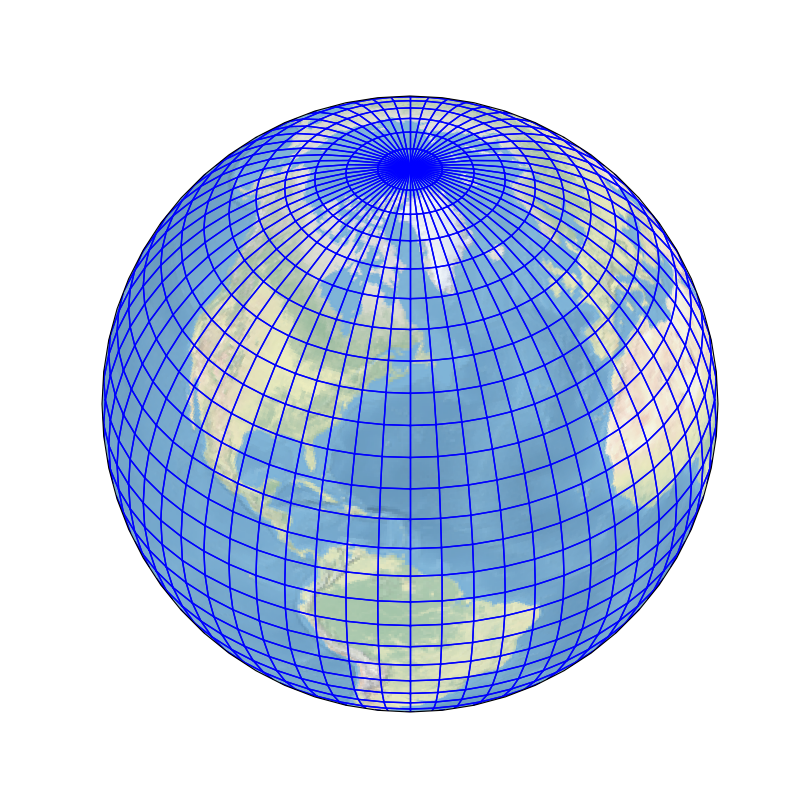
\includegraphics[width = \linewidth]{latlon_sphere}
		\caption{Latitude-longitude grid}\label{latlon-grid}
	\end{subfigure}%
  \hspace{1em}% Space between image A and B
\begin{subfigure}{.3\linewidth}
	\centering
	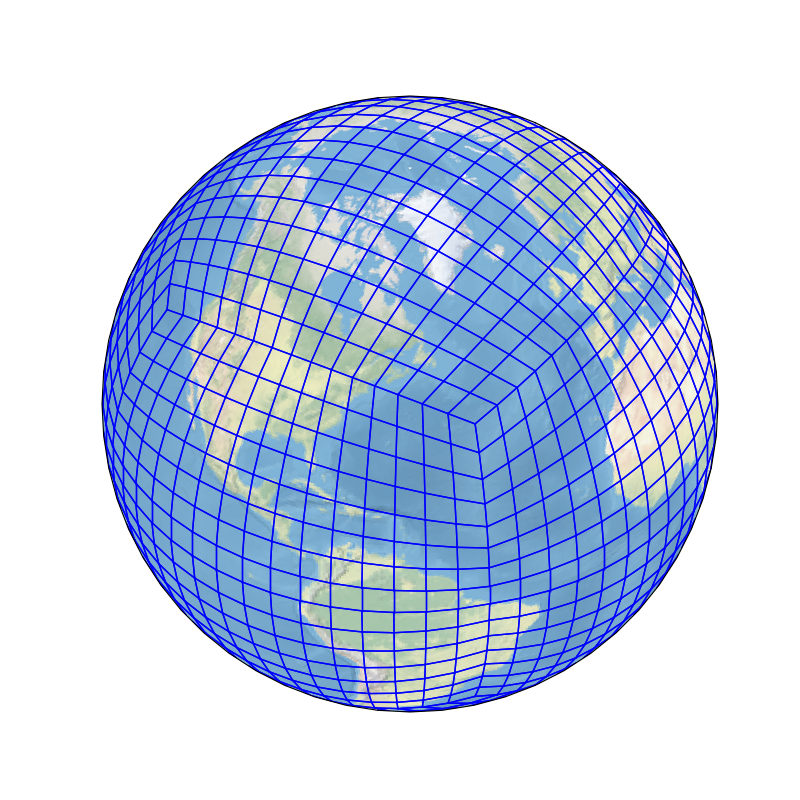
\includegraphics[width = \linewidth]{gnomonic_equiangular_15_sphere}
	\caption{Cubed-sphere}\label{cs-grid}
\end{subfigure}%
	\hspace{2em}% Space between image B and C
	\begin{subfigure}{.3\linewidth}
		\centering
		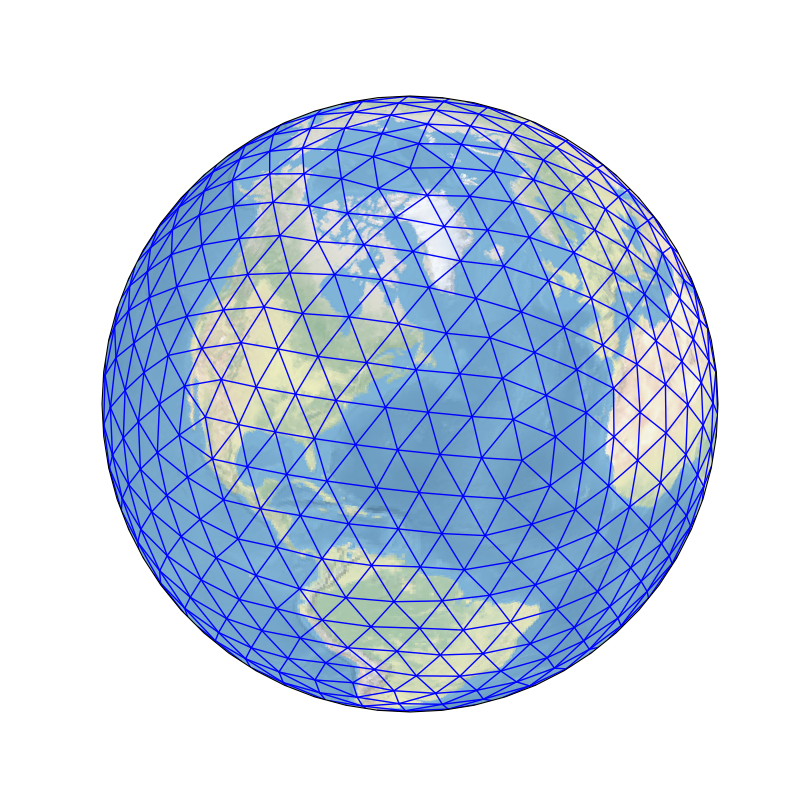
\includegraphics[width = \linewidth]{icos_pol_nopt_3_edsphere}
		\caption{Icosahedral grid}\label{icos-grid}
	\end{subfigure}
	\begin{subfigure}{.3\linewidth}
		\centering
		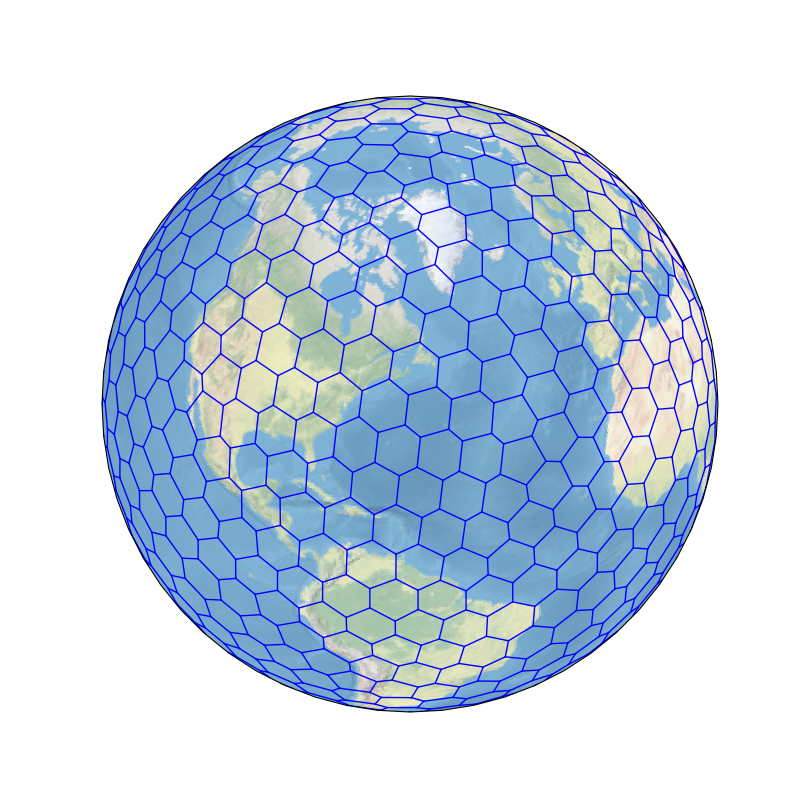
\includegraphics[width = \linewidth]{icos_pol_nopt_3_edhxsphere}
		\caption{Pentagonal/Hexagonal grid}\label{voronoi-grid}
	\end{subfigure}
	\begin{subfigure}{.3\linewidth}
		\centering
		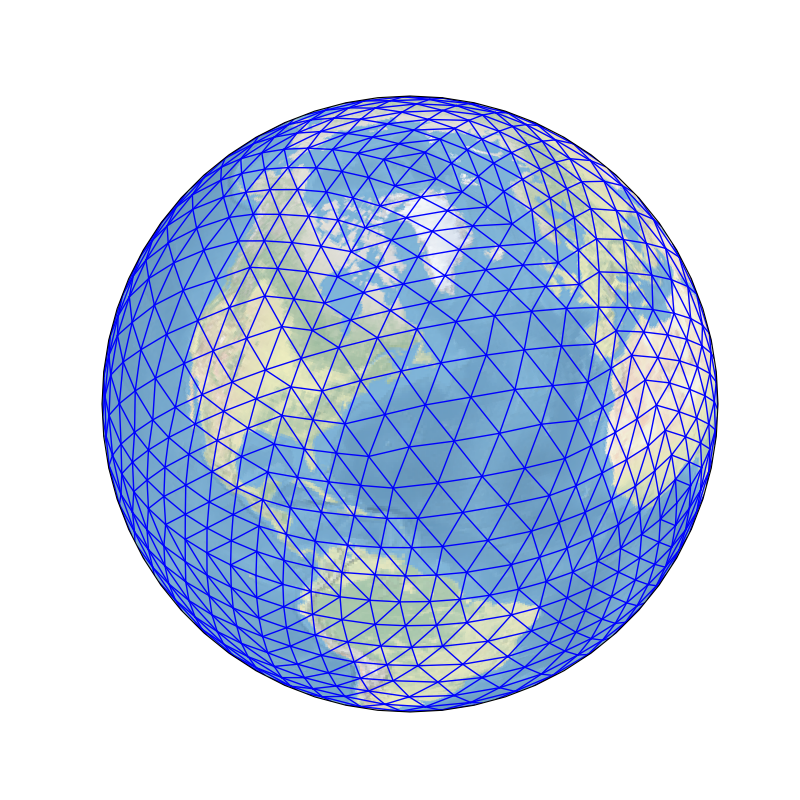
\includegraphics[width = \linewidth]{octg_pol_nopt_4_edsphere}
		\caption{Octahedral grid}\label{octg-grid}
	\end{subfigure}
	\caption{Examples of spherical grids: latitude-longitude grid (a) and grids based on Platonic solids (b)-(d).}
\end{figure}

The emergence of the Fast Fourier Transform (FFT) in the 1960s with the work from 
\citet{cooley:1965} allowed the computation of discrete Fourier transforms with
$N\log(N)$ complexity. 
The viability of the usage of FFTs for solving atmospheric flows was shown by \citet{orszag:1970},
using the barotropic vorticity equation on the sphere, and by \citet{eliasen:1970}, using
the primitive equations.
The spectral transform method expresses latitude-longitude grid values, that represent some scalar field,
using truncated spherical harmonics expansions, which consists of Fourier expansions 
in latitude circles and Legendre functions expansions in longitude circles. 
The coefficients in the spectral expansions are known
as spectral coefficients and are usually thought to live in the so-called spectral space.
Given the grid values, the spectral coefficients are obtained by performing a FFT followed by a 
Legendre Transform (LT). 
Conversely, given the spectral coefficients,
the grid values are obtained by performing an inverse LT followed by an inverse FFT.
The main idea of the spectral method is to apply the spectral transform, in order to 
go the spectral space, and evaluate spatial derivatives in the spectral space, which
consists of multiplying the spectral coefficients by constants. 
Then, the method performs the inverse spectral transform
in order to get back to grid space, and the nonlinear terms are treated on the grid space
\citep{krishnamurti:2006}.

The spectral transform makes the use of SI-SL methods computationally cheap, 
since the solution to elliptic problems becomes easy, once the spherical harmonics are
eigenfunctions of the Laplacian operator on the sphere.
Therefore, the spectral transform method gets faster when combined with the SI-SL approach
due to the larger times-steps allowed in this case.
Due to these enhancements, the spectral transform dominated global atmospheric modeling 
\citep{randall:2018} since the 1980s.
Indeed, the spectral method is still used in many current operational Weather Forecasting models such as
the Integrated Forecast System (IFS) from  European Centre for Medium-Range Weather Forecasts (ECMWF),
Global Forecast System (GFS) from National Centers for Environmental Prediction (NCEP) and the
Brazilian Global Atmospheric Model (BAM) \citep{figueroa:2016} from  Center for Weather Forecasting 
and Climate Research [Centro de Previsão de Tempo e Estudos Climáticos (CPTEC)].

With the beginning of the multicore era in the 1990s, the global atmospheric models
started to move towards parallel efficiency aiming to run at very high resolutions. 
Even though the spectral transform expansions have a global data dependency, some parallelization
is feasible among all the computations of FFTs, LTs and their inverses \citep{barros:1995}.
However, the parallelization of the spectral method requires data transpositions in order
to compute FFTs and LTs in parallel.  
These transpositions demand a lot of global communication using, for instance,
the Message Passing Interface (MPI) \citep{zheng:2018}. 
Indeed, the spectral transform becomes the most expensive component of global spectral models
when the resolution is increased due to the amount of MPI communications \citep{mueller:2019}.

The adiabatic and frictionless continuous equations that govern the atmospheric flow have 
conserved quantities. Among them, some of the most important are mass, total energy, 
angular momentum and potential vorticity \citep{thuburn:2011}.
Numerical schemes that are known for having discrete analogous of these conservative properties
are known as mimetic schemes.
As we pointed out, Semi-Lagrangian schemes lack mass conservation. Nevertheless, 
these schemes have been employed in dynamical cores for better computational performance.
However, dynamical cores should have discrete analogous of the 
continuous conserved quantities, especially concerning for longer simulation runs.

Aiming for better performance in massively parallel computers and conservation properties, 
new dynamical cores have been developed since the beginning of the 2000s.
Novel spherical grids have been proposed, in order to avoid the pole problem.
A popular choice are grids based on Platonic solids \citep{stan:2012}.
The construction of these grids relies on a Platonic circumscribed on the sphere and 
the projection of its faces onto the sphere, which leads to quasi-uniform and more isotropic
spherical grids.
Some examples of spherical grids based on Platonic solids employed in the new generation
of dynamical cores are the cubed-sphere (Figure \ref{cs-grid}), icosahedral grid (Figure \ref{icos-grid}), 
the pentagonal/hexagonal or Voronoi grid (Figure \ref{voronoi-grid}) and octahedral grid (Figure \ref{octg-grid}),
which are based on the cube, icosahedron, dodecahedron and octahedron, respectively \citep{ullrich:2017}.

\section{Motivations and the FV3 model}
The cubed-sphere became a popular quasi-uniform grid for the new generation of dynamical cores.
It was originally proposed by \citet{sadourny:1972} and it was revisited by \citet{ronchi:1996}.
Some of the cubed-sphere advantages are: uniformity; quadrilateral structure, 
making the grid indexing trivial; no overlappings; it is cheap to generate.
However, the major drawbacks of the cubed-sphere are: non-orthogonal coordinate system, which
leads to metric terms on the differential operators; discontinuity of the coordinate system
at the cube edges, which may generate numerical noise and
demands special treatment of discrete operators at the cube edges.

Despite of its drawbacks, the cubed-sphere has been adopted in some of the new generation
dynamical cores.
For instance, the cubed-sphere is used in the 
Community Atmosphere Model (CAM-SE) from the NCAR using spectral elements \citep{dennis:2012} and in the
Nonhydrostatic Unified Model of the Atmosphere (NUMA) from the US Navy using Discontinuous Galerkin 
methods \citep{giraldo:2013}. The cubed-sphere was also chosen to be used in the next UK Met Office
global model using mixed finite elements \citep{melvin:2022}.
At last, the Finite­ Volume Cubed-Sphere dynamical core (FV3) from the Geophysical Fluid 
Dynamics Laboratory (GFDL) and the National Oceanic and Atmospheric Administration (NOAA)
\citep{putman:2007,harris:2013} is another example
of new generation dynamical core based on the cubed-sphere.

The FV3 dynamical core is an extension of the Finite-Volume dynamical core (FVcore)
from latitude-longitude grids to the cubed-sphere.
The numerical methods from FVcore started to be developed with the advection scheme from the work \citet{lin:1994},
which is based on the piecewise linear scheme from \citet{vanleer:1977}. 
This scheme was later improved, using the Piecewise Parabolic Method (PPM) \citep{colella:1984, carpenter:1990}
using dimension splitting techniques that guarantee monotonicity and mass conservation,
for the advection equation \citep{lin:1996} and the shallow-water equations \citep{lin:1997}. 
An important feature is that the FVcore combines the  Arakawa C- and D-grids \citep{arakawa:1977},
where the C-grid values are computed in and intermediate time step. 
The full global model was then presented by \citet{lin:2004}.

A computational disadvantage of the FVcore is its Semi-Lagrangian formulation that creates more demand
for MPI communication when computing the accumulated fluxes \citep{lin:1996}.
The FVcore was then adapted to the cubed-sphere grid \citep{putmanthesis:2007, putman:2007}, 
to reach better performance in parallel computers, leading to the FV3 model.
Later, the FV3 also was improved to allow locally refinement grids 
through grid-nesting or grid-stretching \citep{harris:2013}.

Currently, the FV3 model is capable of perfoming hydrostatic and non-hydrostatic atmospheric simulations 
and it was chosen as the new US global weather prediction model, indeed, it replaced the spectral transform
Global Forecast System (GFS) in June, 2019
(\url{https://www.noaa.gov/media-release/noaa-upgrades-us-global-weather-forecast-model}, last access: 19th of March, 2024).
Additionally, the FV3 dynamical core is employed in the GEOS Chem model \citep{martin:2022} from Harvard University, 
in NASA’s next-generation Mars Climate Model \citep{wilson:2022}, 
and also in the System for High-resolution prediction on Earth-to-Local Domain (SHiELD) model from GFDL \citep{harris:2020}.

However, a well-known problem that occurs on cubed-sphere models that use low-order numerical methods
is the grid imprinting visible due to the coordinate system discontinuity, 
especially at larger scales, leading to the emergence of a wavenumber 4 pattern.
This was reported in the paper of \citet{rancic:2017}, where the authors employ a 
finite-difference numerical scheme on the Uniform Jacobian cubed-sphere using a Arakawa B-grid.
The unpublished report from \citet{whitaker:2015} shows grid imprinting in other models, including 
the FV3.
More recently, \citet{mouallem:2023} has shown some idealized simulations using FV3 where grid imprinting appears in many simulations.
Generally speaking, grid imprinting refers to the presence of artificial behaviors in the numerical solution that are associated with the grid used.
It is important to emphasize that other quasi-uniform grids may also experience grid imprinting, such as hexagonal grids \citep{weller:2012, peixoto:2013, peixoto:2016}.

Despite being chosen as the new US global weather prediction model, there is a lack of numerical studies on the FV3 discretizations in the literature.
Numerical results for the advection equation on the cubed-sphere using the FV3 dynamical core were presented in \citet{putman:2007}.
However, they utilized extrapolations near the cube edges instead of the duo-grid approach from \citet{mouallem:2023}, which affects the convergence of this method.
The current solver of FV3 solves the shallow-water equation on the so-called Lagrangian surfaces.
This shallow-water solver, based on \citet{lin:1997}, 
utilizes the advection solver from \citet{putman:2007} to update the pressure, vorticity, and kinetic energy fluxes.
Therefore, advection is a key aspect of the FV3 dynamical core and it deserves to be better understood.
Although \citet{mouallem:2023} present results on the convergence of some shallow-water tests,
they do not provide a detailed discussion on the solver on the cubed-sphere itself.
Therefore, in this thesis, we propose to thoroughly examine all the minor details of the scheme from \citet{putman:2007} and suggest potential improvements,
thus addressing gaps in the existing literature.


\section{Outline and contributions}
This thesis is outlined as follows.
\begin{itemize}
\item Chapter \ref{chp-1d-fv} is dedicated to reviewing the Piecewise Parabolic Method (PPM) for the one-dimensional advection equation. 
In this Chapter, we demonstrate how the temporal component of PPM can be expressed as a departure point calculation. 
Subsequently, we enhance the departure point calculation from first-order (which is utilized in FV3) to second-order.
This enhancement results in a significant improvement, particularly in non-constant wind simulations.
Its benefits are also observed when using the monotonic version of PPM used in FV3 and proposed by \citet{lin:2004}.
The additional cost is only due to linear interpolation, which has little impact on the overall performance.

\item Chapter \ref{chp-2d-fv} reviews the dimension splitting method, which allows us to use one-dimensional methods, 
such as the PPM, to solve the two-dimensional advection equation. 
We review the current 2D advection scheme of FV3 on the plane proposed by \citet{putman:2007}.
The main feature of this scheme is that it preserves a constant scalar field when the wind is divergence-free.
We show through some numerical simulations that this scheme is second-order accurate only for divergence-free winds.
When the wind is not divergence-free, we show that this scheme is only first-order accurate.
On the other hand, we propose a small modification of the \citet{putman:2007} scheme 
using the second-order departure point computation presented in Chapter \ref{chp-1d-fv},
which allows us to achieve second-order accuracy and smaller errors for both divergent and divergence-free winds. 
Despite this scheme not preserving a constant scalar for divergence-free winds, it still exhibits second-order error in this case as well. 
Furthermore, when the monotonic scheme is used in the 1D solver, this scheme also has smaller errors compared to the \citet{putman:2007} scheme.

\item In Chapter \ref{chp-cs-grids}, we introduce the cubed-sphere grid utilized in FV3, 
which includes the equi-edge \citep{chen:2021} and equiangular grids \citep{ronchi:1996}, 
and we investigate their geometrical properties.
Next, we present all the tools necessary to extend the advection schemes on the plane from Chapter \ref{chp-2d-fv} to the sphere.
We review the contravariant/covariant wind formulation induced by the cubed-sphere mappings.
Additionally, we demonstrate how stencils can be computed near the cube-edges through the duo-grid 
technique to generate the ghost cells required for utilizing 1D Lagrange interpolation to fill these ghost cells.


\item Chapter \ref{chp-cs-fv} extends the ideas of Chapter \ref{chp-2d-fv} to the cubed-sphere grid using the tools from Chapter \ref{chp-cs-grids}.
The dimension-splitting method on each cubed-sphere panel works as in the plane, 
with the addition of metric terms due to the non-orthogonality of the grid and interpolation between panels to obtain ghost cell values needed for stencil computations. 
We show that the scheme from \citet{putman:2007} uses a less accurate formulation of the metric term to preserve the constant scalar for a divergence-free wind,
while our new scheme may use a more accurate formulation of the metric term, as it does not have this preservation constraint. 
The results are essentially the same as those from Chapter \ref{chp-2d-fv}, 
showing that our scheme successfully extends from the plane to the cubed-sphere and is more accurate. 
We also demonstrate that our new scheme has smaller errors at the corners compared to the scheme from \citet{putman:2007}.
\end{itemize}

In summary, the main contribution of this thesis is a modified version of the two-dimensional scheme proposed by \citet{putman:2007}, which exhibits improved accuracy.
We give some final thoughts and future work perspectives in Chapter \ref{chp-conclusions}.
\chapter{One-dimensional finite-volume methods}
\label{chp-1d-fv}

\theoremstyle{plain}
\newtheorem{lema}{Lemma}[chapter]

\theoremstyle{plain}
\newtheorem{prop}{Proposition}[chapter]

\theoremstyle{plain}
\newtheorem{thrm}{Theorem}[chapter]

\theoremstyle{plain}
\newtheorem{remark}{Remark}[chapter]

\theoremstyle{plain}
\newtheorem{corollary}{Corollary}[chapter]

\theoremstyle{plain}
\newtheorem{definition}{Definition}[chapter]


The aim of this chapter is to provide a detailed description of one-dimensional (1D) 
finite-volume (FV) schemes within a Semi-Lagrangian (SL) framework, specifically applied to 
the 1D advection equation.
These schemes are also known as flux-form Semi-Lagrangian schemes, and they allow for time steps beyond the 
Courant-Friedrichs-Lewy (CFL) condition while preserving the total mass.
FV-SL schemes have been explored in the literature since the work of  \citet{leveque:1985},
which extended the finite-volume schemes from \citet{godunov:1959}  to accommodate larger time steps.
This approach has been further investigated in the literature (c.f, e.g. . \citet{lin:1996,leonard:1996}).
We are going to focus on the linear advection equation because in FV3, the horizontal dynamics
are solved by using flux advection operators to compute the fluid density, absolute vorticity, 
and the kinetic energy \citep{lin:1997,putmanthesis:2007, harris:2013, harris:2021}.
The boundary conditions are assumed to be periodic for simplicity.

To introduce the FV-SL schemes, we begin by discretizing the spatial and temporal domains into uniform grids.
Subsequently, the FV-SL schemes involve three steps.
The first step involves computing the departure points of the spatial grid edges.
The second step, known as reconstruction, utilizes the grid cell average values to
determine a piecewise function within each cell. This piecewise function approximates the
values of the advected quantity and ensures the preservation of its local mass within each grid cell.
The third step involves updating the fluxes at the grid edges by integrating the reconstruction function 
over a domain that extends from the departure point of the grid edge to the grid edge itself.

The first step of FV-SL schemes can be accomplished by integrating an ordinary differential
equation backward in time.
The second step is performed using the Piecewise-Parabolic Method (PPM) proposed by \citet{colella:1984}.
As the name suggests, PPM employs piecewise-parabolic functions.
The third and final step is computed easily, as the reconstruction functions consist of parabolas that preserve the local mass.

It is worth noting that the reconstruction function can be constructed using functions other than parabolas.
In fact, PPM can be seen as an
extension of the Piecewise-Linear method proposed by \citet{vanleer:1977}, which,
in turn, was inspired by the Piecewise-Constant method introduced by \citet{godunov:1959}. 
Additionally, other schemes inspired by PPM have been proposed in the literature utilizing
higher-order polynomials, such as quartic polynomials \citep{white:2008}. For a
comprehensive review of general piecewise-polynomial reconstruction, we recommend
referring to the technical report by \citet{engwirda:2016}, \citet{lauritzen:2011}, and the
references therein.

The PPM approach has become popular in the literature for gas dynamics simulations, astrophysical 
phenomena modeling \citep{woodward:1986}, and later on atmospheric simulations \citep{carpenter:1990}. 
Indeed, PPM has been implemented in the FV3 dynamical core on its latitude-longitude grid \citep{lin:2004}
and cubed-sphere \citep{putman:2007} versions.
Although many other shapes for the basis functions and higher-order schemes are available in the literature, 
\citet{harris:2021} points out that the PPM scheme suits the needs of FV3 well. It is a flexible method that
can be modified to ensure low diffusivity or shape preservation, for example.
Additionally, a finite-volume numerical method usually requires monotonicity constraints, which, according 
to Godunov's order barrier theorem \citep{wesseling:2001}, limit the order of convergence to at most 1. 
Therefore, a higher-order scheme needs to strike a well-balanced trade-off between increasing computational 
cost and potential benefits.

This chapter begins with a basic review of one-dimensional advection equation in the integral form
in Section \ref{chp-adv1d-sec1}. In Section \ref{chp-adv1d-sec2-fvsl}, we establish the framework for general
one-dimensional finite-volume Semi-Lagrangian schemes. Section \ref{chp-adv1d-sec-dp} presents
methods for computing the departure point. The PPM reconstruction is described in Section \ref{chp-adv1d-sec-recon},
while Subsection \ref{chp-adv1d-sec-mono} introduces different approaches to ensure the monotonicity of parabolas.
Section \ref{chp-adv1d-sec-flux} focuses on the description and investigation of the PPM flux computation.
Section \ref{chp-adv1d-sec-numerical-exp}
presents numerical results using the PPM scheme for the advection equation.
Finally, Section \ref{chp-adv1d-sec-conclusion} presents some concluding remarks.
The application of PPM to solve two-dimensional problems will be addressed in Chapter \ref{chp-2d-fv}.

\section{One-dimensional advection equation in integral form}
\label{chp-adv1d-sec1}

\subsection{Notation}
\label{chp-adv1d-sec-not}
Before introducing the FV-SL schemes, let us establish some notation by introducing
the concepts of a $\Delta x$-grid, a $\Delta t$-temporal grid, and the
$(\Delta x, \Delta t, \lambda)$-discretization, as well as the concept of grid function/winds.
In this chapter, we will use the notation $\Omega=[a,b]$ to represent the interval under consideration,
and $\nu$ to represent a non-negative integer indicating the number of ghost cell layers in each boundary.
We also use the notations $\mathbb{R}^{N}_{\nu}:=\mathbb{R}^{N+2\nu}$ and
$\mathbb{R}^{N+1}_{\nu}:=\mathbb{R}^{N+1+2\nu}$.
\begin{definition}[$\Delta x$-grid]\label{chp-adv1d-def-dxgrid}
	For a given interval $\Omega$ and a positive real number $\Delta x$ such that 
    $\Delta x = (b-a)/N$ for some positive integer $N$, 
	we say that $\Omega_{\Delta x}= \{X_i \}_{i=-\nu+1}^{N+\nu}$ is a $\Delta x$-grid for $\Omega$ if
	\begin{align*}
        X_i = [x_{i-\frac{1}{2}},x_{i+\frac{1}{2}}] = [a+(i-1)\Delta x, a+i\Delta x],
    \end{align*}
	and $\Delta x = x_{i+\frac{1}{2}} - x_{i-\frac{1}{2}}$. 
	Each $X_i$ is referred to as a control volume or cell, and $x_{i-\frac{1}{2}}$ and 
	$x_{i+\frac{1}{2}}$ are the edges of the control volume $X_i$.
	The cell centroid is defined by
    \begin{align*}
    x_i = \frac{1}{2}(x_{i+\frac{1}{2}} + x_{i-\frac{1}{2}}),\quad \forall i = -\nu+1, \ldots, N+\nu,
    \end{align*}
	and $\Delta x$ is the cell length.
\end{definition}
\begin{remark}
If $1 \leq i \leq N$, we refer to $i$ as an interior index;
otherwise, $i$ is considered a ghost cell index and we say the $X_i$ is a ghost cell.
\end{remark}

\begin{figure}[!htb]
	\centering
	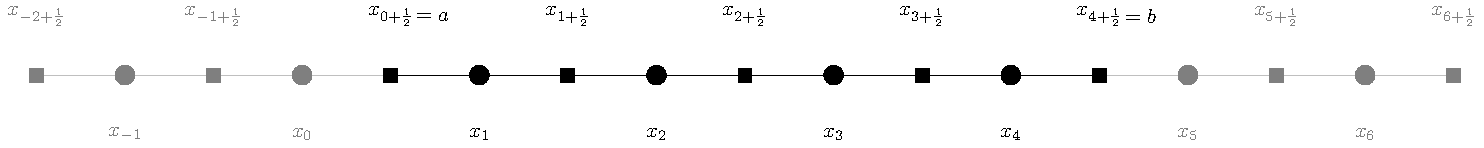
\includegraphics[width=1\linewidth]{1d_grid}
	\caption{Illustration of a $\Delta x$-grid with $N=4$ cells in its interior (in black) 
         and $\nu=2$ ghost cell layers (in gray).
	 The edges are denoted by squares and the cell centroids are denoted using circles.\label{chp-adv1d-sec1-grid1d}}
\end{figure}

\begin{definition}[$\Delta t$-temporal grid]
	For a given interval $[0,T]$ and a positive real number $\Delta t$ such that $\Delta t = T/N_T$
    for some positive integer $N_T$, we say that  $T_{\Delta T}= \{T_n\}_{n=0}^{N_T}$ a $\Delta t$-temporal grid for $[0,T]$ if
    \begin{align*}
	T_n = [t^n, t^{n+1}], \quad t^n = n\Delta t, \quad \Delta t = \frac{T}{N_T}, \quad \forall n = 0, \ldots, N_T.
    \end{align*}
    In this context, we also define $t^{n+\frac{1}{2}} = \frac{t^n+t^{n+1}}{2}$.
\end{definition}

\begin{definition}[$(\Delta x,\Delta t, \lambda)$-discretization]
\label{chp-adv1d-def-dxtimegrid}
	Given $\Omega \times [0,T]$ and positive real numbers $\Delta x$ and $\Delta t$,
    we say that $(\Omega_{\Delta x}, T_{\Delta t})$ is a $(\Delta x, \Delta t, \lambda)$-discretization 
    of $\Omega \times [0,T]$ if $\Omega_{\Delta x}$ is a $\Delta x$-grid for $\Omega$, 
    ${T}_{\Delta t}$ is a $\Delta t$-temporal grid for $[0,T]$, and $\frac{\Delta t}{\Delta x} = \lambda$.
\end{definition}
\begin{remark}
	Whenever we refer to a $\Delta x$-grid, a $\Delta t$-temporal grid, or a $(\Delta x, \Delta t, \lambda)$-discretization, 
	$X_i$, $N$, $t^n$, and $N_T$ are assumed to be implicitly defined.
\end{remark}
Next, we introduce the definitions of grid functions at cell centroids and edges.
\begin{definition}[$\Delta x$-grid function]
	For a $\Delta x$-grid, we say that $Q$ is a $\Delta x$-grid function if
	$Q = (Q_{-\nu+1}, \ldots, Q_{N+\nu}) \in \mathbb{R}^{N}_{\nu}$.
\end{definition}
\begin{definition}[$\Delta x$-grid wind]
	For a $\Delta x$-grid, we say that $u$ is a $\Delta x$-grid wind if
	$u = (u_{-\nu+\frac{1}{2}}, \ldots, u_{N+\nu+\frac{1}{2}}) \in \mathbb{R}^{N+1}_{\nu}$.
\end{definition}
The definition of a $\Delta x$-grid wind is based on the Arakawa grids \citep{arakawa:1977}.
Considering functions $q, u: \Omega \times[0,T] \to \mathbb{R}$ and a $(\Delta x,\Delta t, \lambda)$-discretization
of $\Omega \times[0,T]$, we introduce the grid functions $q^n \in \mathbb{R}^{N}_{\nu}$ and $u^n \in \mathbb{R}^{N+1}_{\nu}$
where ${q}^n_{i} \approx {q}(x_i, t^{n})$ and $u^n_{i+\frac{1}{2}} = u(x_{i+\frac{1}{2}},t^n)$.
The grid function $q^n$ approximate the discrete values of $q$ at cell centroids and $u^n$ represents the values of $u$ approximates edges, both
for each time level $t^n$ (Figure \ref{chp-adv1d-sec1-grid1d-function}).


In this Chapter, our focus lies on periodic grid functions.
We define a $\Delta x$-grid function $Q$ as periodic if it satisfies the following conditions:
\begin{align*}
    Q_{i} &= Q_{N+i}, \quad i=-\nu+1, \ldots, 0,\\
    Q_{i} &= Q_{i-N}, \quad i=N+1, \ldots, N+\nu.
\end{align*}
Similarly, we define a $\Delta x$-grid wind as periodic if it meets the following requirements:
\begin{align*}
    u_{i-\frac{1}{2}} &= u_{N+i+\frac{1}{2}} , \quad i=-\nu, \ldots, -1,\\
    u_{i+\frac{1}{2}} &= u_{i+\frac{1}{2}-N} , \quad i=N+1, \ldots, N+\nu.
\end{align*}
We use the notation $\mathbb{P}^{N}_{\nu}$ and $\mathbb{P}^{N+1}_{\nu}$ to
represent the spaces of periodic $\Delta x$-grid functions and winds, respectively.
\begin{figure}[!htb] 
\centering 
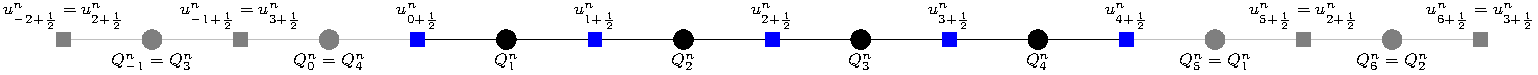
\includegraphics[width=1\linewidth]{1d_grid_function} 
\caption{Illustration of $\Delta x$-grid function $Q$ (black circles)
and a $\Delta x$-grid wind $u$ (blue squares) and its ghost cell
values (in gray) assuming periodicity.\label{chp-adv1d-sec1-grid1d-function}}
\end{figure}

Given $Q \in \mathbb{P}^{N}_{\nu}$, we define the $p$-norm as
\begin{equation}
	\label{chp-adv1d-sec-not1}
	\|Q\|_{p,\Delta x}=
	\begin{cases}
		\bigg( \sum_{i=1}^{N} |Q_i|^p \bigg)^{\frac{1}{p}} & \text{if } 1\leq p < \infty,\\
		\max_{i=1, \ldots, N}{|Q_i|} & \text{otherwise },
	\end{cases}
\end{equation}
which is indeed a norm for periodic grid functions.
Using a similar notation as in \citet{engwirda:2016}, we define the stencil and a grid function evaluated on a stencil as follows.
\begin{definition}[Stencil]
	For a $\Delta x$-grid, and each $i = 0, \ldots, N$, we define a stencil as a set of the form
	$\mathcal{S}_{i+\frac{1}{2}} = \{i-r+1, \ldots, i-1, i, i+1, \ldots, i+s\} \subset\{-\nu+1, \ldots, N+\nu\}$.
\end{definition}
\begin{definition}[Grid function restricted to a stencil]
	For a $\Delta x$-grid, a stencil $\mathcal{S}_{i+\frac{1}{2}}$,
	 and a $\Delta x$-grid function $Q$, we define $Q(\mathcal{S}_{i+\frac{1}{2}}) = (Q_k)_{k \in \mathcal{S}_{i+\frac{1}{2}}}$.
\end{definition}
These definitions provide the necessary notation for describing grid functions and their evaluations on stencils.
To achieve a more compact notation in some situations, we introduce the centered difference notation:
\begin{equation}
    \label{chp-adv1d-sec-adv-eq5}
	\delta_x {g}(x_i,t) = 
	{g}(x_{i+\frac{1}{2}},t) - 
	{g}(x_{i-\frac{1}{2}},t),
\end{equation}
for any function $g: \Omega \times [0,T] \to \mathbb{R}$.
Additionally, we introduce the average value of $q$ in the $i$-th control volume at time $t$, denoted as ${Q}_i(t)$, defined by:
\begin{equation}
	\label{chp-adv1d-sec1-not2}
	{Q}_i(t) = \frac{1}{\Delta x} \int_{x_{i-\frac{1}{2}}}^{x_{i+\frac{1}{2}}} {q}(x,t) \,dx.
\end{equation}
Moreover, we define the $\Delta x$-grid function of average values as $Q(t) = (Q_i(t))_{i=-\nu+1}^{N+\nu}$.
Here, $Q_i(t)$ represents the average value of $q$ in the $i$-th control volume at time $t$.

For the consideration of periodic boundary conditions, we can define spaces of periodic functions over 
the interval $\Omega$ as follows:
\begin{align*}
	\mathcal{S}_P(\Omega) &= \{q:\mathbb{R}\times[0,+\infty[\to \mathbb{R}: q(x+b-a,t)=q(x,t), \quad \forall x \in \mathbb{R}, \quad t\geq0\}.
\end{align*}
Similarly, the space of $k$-times periodically differentiable functions $\mathcal{C}_P^k(\Omega)$ can be defined as:
\begin{align*}
	\mathcal{C}_P^k(\Omega) &= \mathcal{S}_P(\Omega)\cap \mathcal{C}^k(\mathbb{R}\times[0,\infty[),
\end{align*}
where $\mathcal{C}^k(\mathbb{R}\times[0,+\infty[)$ denotes the space of functions that are $k$ 
times continuously differentiable in both the spatial and temporal variables.
In summary, $\mathcal{S}_P(\Omega)$ represents the space of periodic functions, and $\mathcal{C}_P^k(\Omega)$
represents the space of $k$-times periodically differentiable functions over the interval $\Omega$ subject to periodic boundary conditions.

\subsection{The 1D advection equation}
In this section, we will derive the integral form of the 1D advection equation with periodic boundary conditions over the interval $\Omega$.
What is going to be presented here follows \citet{leveque:1990,leveque:2002} closely.
The advection equation with periodic boundary conditions in its differential form is given by:
\begin{equation}
	\label{chp-adv1d-sec-adv-eq1}
	\begin{cases}
		[{\partial_t q} + {\partial_x (uq)}](x, t)
		= 0, \quad \forall (x,t) \in \mathbb{R}\times ]0, +\infty[,\\
		{q}(a, t) = {q}(b, t), \quad \forall t\geq 0,\\
		q_0(x) = q(x,0), \quad \forall x \in \Omega.
	\end{cases}
\end{equation}
Here, $q \in \mathcal{C}_P^1{(\Omega)}$ represents the advected quantity, and $u \in \mathcal{C}_P^1{(\Omega)}$ represents the velocity.
We will focus on Equation \eqref{chp-adv1d-sec-adv-eq1} over the domain $D = \Omega\times[0,T]$, where $T>0$ is a finite time.
A strong or classical solution to the advection equation is defined as a function ${q}\in\mathcal{C}^1_P(\Omega)$ 
and satisfies Equation \eqref{chp-adv1d-sec-adv-eq1}.
In order to deduce the integral form of Equation \eqref{chp-adv1d-sec-adv-eq1}, we consider
$[x_1, x_2]\times[t_1,t_2]\subset D$. 
Integrating Equation \eqref{chp-adv1d-sec-adv-eq2} over $[x_1, x_2]$, we obtain:
\begin{equation}
    \label{chp-adv1d-sec-adv-eq2}
	\frac{d}{dt} \int_{x_1}^{x_2} q(x,t) \,dx =  
	-({(uq)}(x_2,t) - {(uq)}(x_1,t)) ,
\end{equation}
and integrating Equation \eqref{chp-adv1d-sec-adv-eq2} over $[t_1,t_2]$, we get
\begin{equation}
    \label{chp-adv1d-sec-adv-eq3}
    \int_{x_1}^{x_2} q(x,t_2) \,dx=  \int_{x_1}^{x_2} q(x,t_1)
	-\bigg( \int_{t_1}^{t_2} 
	{(uq)}(x_2, t) \,dt - 
	\int_{t_1}^{t_2}{(uq)}(x_1, t) \,dt \bigg).
\end{equation}
The presented problem, Problem \ref{chp-adv1d-sec2-prob1}, aims to find a solution, called weak solution, to the advection equation
in its integral form, considering the given initial condition ${q}_0$ and velocity function $u$.

\theoremstyle{plain}
\newtheorem{prob}{Problem}[chapter]
\begin{prob}
	\label{chp-adv1d-sec2-prob1}
	Given an initial condition ${q}_0$ and a velocity function $u$  we would like to find a weak solution ${q}$
	of the advection equation in the integral form:
	\begin{equation*}
	        \int_{x_1}^{x_2} {q}(x, t_2) \,dx =
       		\int_{x_1}^{x_2} {q}(x, t_1) \,dx +
        	\int_{t_1}^{t_2} {(uq)}(x_1, t) \,dt -
		\int_{t_1}^{t_2}{(uq)}(x_2, t) \,dt ,
	\end{equation*}
	$\forall [x_1, x_2]\times[t_1, t_2] \subset \Omega \times [0,T]$,
	and
	${q}(x,0) = {q}_0(x)$, $\forall x \in \Omega$, $q(a,t)=q(b,t)$, $\forall t \in [0,T]$.
\end{prob}
We point out that, for Problem \ref{chp-adv1d-sec2-prob1}, the total mass in $\Omega$ at time $t$ defined by:
\begin{equation*}
{M}_{[a,b]}(t) = \int_{a}^{b} q(x,t) \,dx,
\end{equation*}
remains constant over time, i.e.,
\begin{equation*}
	{M}_{[a,b]}(t) = {M}_{[a,b]}(0), \quad \forall t \in [0,T].
\end{equation*}
This conservation of total mass property is highly desirable for numerical schemes aiming
to approximate general conservation law solutions accurately.

Applying the steps from Equation \eqref{chp-adv1d-sec-adv-eq1} to Equation \eqref{chp-adv1d-sec-adv-eq3} in reverse order,
one can verify that if ${q}$ is a weak solution and $q \in \mathcal{C}^1_P{(\Omega)}$, then it satisfies Equation \eqref{chp-adv1d-sec-adv-eq1}.
Therefore, Equation \eqref{chp-adv1d-sec-adv-eq1} and Problem \eqref{chp-adv1d-sec2-prob1} are equivalent when $q \in \mathcal{C}^1_P{(\Omega)}$.
However, Problem \eqref{chp-adv1d-sec2-prob1} can be formulated for functions that are not $\mathcal{C}^1$ and have discontinuities.
In fact, Problem \eqref{chp-adv1d-sec2-prob1} only requires that $q$ and $uq$ are locally integrable.

It is worth noting that Equation \eqref{chp-adv1d-sec-adv-eq3} holds for all $x_1, x_2, t_1$, and $t_2$ such that $[x_1, x_2]
\times [t_1, t_2] \subset D$. Therefore, let us consider a $(\Delta x, \Delta t, \lambda)$-discretization of $D$ and 
rewrite Equation \eqref{chp-adv1d-sec-adv-eq3} in terms of this discretization. By replacing $t_1, t_2, x_1$, and $x_2$ with
$t^{n}, t^{n+1}, x_{i-\frac{1}{2}}$, and $x_{i+\frac{1}{2}}$, respectively, in Equation \eqref{chp-adv1d-sec-adv-eq3}, we obtain:
\begin{equation}
    \label{chp-adv1d-sec-adv-eq4}
	\begin{aligned}
		{Q}_i(t^{n+1}) =  {Q}_i(t^{n}) -
		\frac{1}{\Delta x}\bigg( \int_{t^{n}}^{t^{n+1}}
        	{(uq)}(x_{i+\frac{1}{2}}, t) \,dt -
		\int_{t^{n}}^{t^{n+1}}{(uq)}(x_{i-\frac{1}{2}}, t) \,dt \bigg), \\
		\quad \forall i = 1, \ldots, N,
		\quad \forall n = 0, \ldots, N_T-1.
	\end{aligned}
\end{equation}
To achieve a more compact notation, we use the centered difference notation
and then Equation \eqref{chp-adv1d-sec-adv-eq4} can be rewritten as:
\begin{equation}
    \label{chp-adv1d-sec-adv-eq6}
    {Q}_i(t^{n+1}) =  {Q}_i(t^{n}) -
	\frac{1}{\Delta x} \delta _x\bigg( \int_{t^{n}}^{t^{n+1}}
        {(uq)}(x_{i}, t) \,dt \bigg),
        \quad \forall i = 1, \ldots, N,
        \quad \forall n = 0, \ldots, N_T-1.
\end{equation}

Now we can define a discretized version of Problem \ref{chp-adv1d-sec2-prob1} as Problem \ref{chp-adv1d-sec2-prob2}.
\begin{prob}
	\label{chp-adv1d-sec2-prob2}
	Let us consider the framework of Problem \ref{chp-adv1d-sec2-prob1} and a $(\Delta x, \Delta t, \lambda)$-discretization of 
	$\Omega \times [0,T]$. Since we are operating within the framework of Problem \ref{chp-adv1d-sec2-prob1}, the following relationship holds:
	\begin{equation}
		\label{1d-fvexact-scheme}
		{Q}_i(t^{n+1}) = {Q}_i(t^{n}) - \lambda \delta_x\bigg( \frac{1}{\Delta t}\int_{t^{n}}^{t^{n+1}}{(uq)}(x_{i}, t) \,dt \bigg),
		 \quad \forall i = 1, \ldots, N, \quad \forall n = 0, \ldots, N_T-1,
	\end{equation}
	where ${Q}_i(t) = \frac{1}{\Delta x}\int_{x_{i-\frac{1}{2}}}^{x_{i+\frac{1}{2}}} {q}(x,t) \,dx$. 
	Our objective now is to determine the values ${Q}_i(t^{n})$, $\forall i = 1, \ldots, N$, $\forall n = 0, \ldots, N_T-1$,
	given the initial values ${Q}_i(0)$, $\forall i = 1, \ldots N$. 
	In other words, we aim to find the average values of ${q}$ in each control volume $X_i$ at the specified time instances.
\end{prob}
It is important to note that no approximations have been made in problems \eqref{chp-adv1d-sec2-prob1} and \eqref{chp-adv1d-sec2-prob2}. 
In Equation \eqref{1d-fvexact-scheme}, we divided and multiplied by $\Delta t$ to interpret
$\frac{1}{\Delta t}\int_{t^{n}}^{t^{n+1}}({uq})(x_{i\pm \frac{1}{2}}, t) \,dt$ 
as a time-averaged flux. This interpretation is useful for deriving finite-volume schemes.

In Problem \ref{chp-adv1d-sec2-prob2}, we need to approximate the time-averaged flux at the cell edges $x_{i\pm\frac{1}{2}}$
to derive a finite-volume scheme. This flux, in principle, requires knowledge of $q$ over the entire interval $[t^n, t^{n+1}]$. 
To overcome this, we can express the temporal integral as a spatial integral at time $t^n$. 
This approach avoids the need for information about $q$ throughout the entire interval $[t^n, t^{n+1}]$. 
Furthermore, this spatial integral domain is closely related to the definition of the 
departure point. 

To introduce the definition of departure point, for each $s \in [t^n,t^{n+1}]$,
we consider the following Cauchy problem backward in time:
\begin{equation}
	\label{chp-sec-flux:analysis-eq3}
	\begin{cases}
		\partial_t x^d_{i+\frac{1}{2}} (t,s) = u(x^d_{i+\frac{1}{2}}(t,s) ,t),\quad t\in[t^{n},s] \\
		x^d_{i+\frac{1}{2}}(s,s) = x_{i+\frac{1}{2}}.
	\end{cases}
\end{equation}
The point $x^d_{i+\frac{1}{2}}(t^n,s)$ is called departure point at time $t^n$
of the point $x_{i+\frac{1}{2}}$ at time $s$.
In Figure \ref{chp-adv1d-sec1-grid1d-dep} we illustrate the departure point idea.

\begin{figure}[!htb]
	\centering
	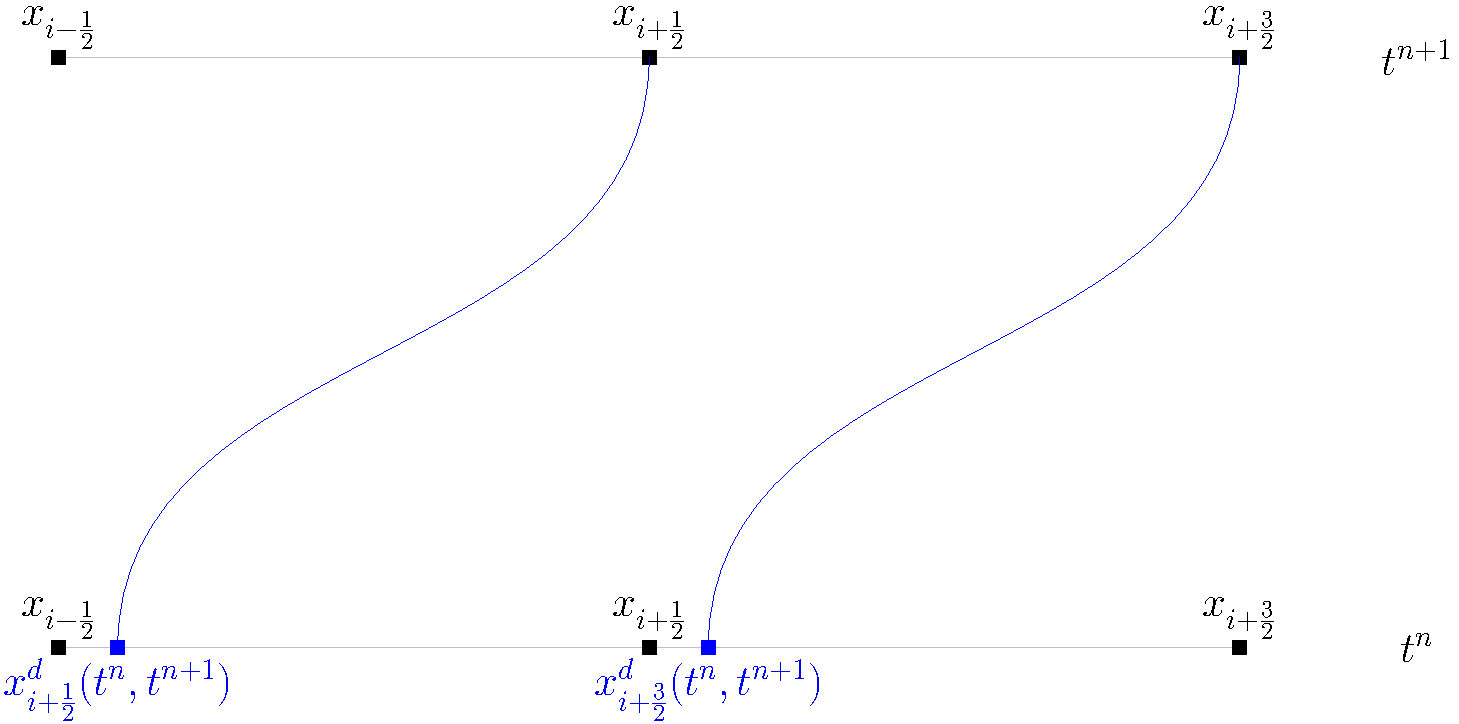
\includegraphics[width=1\linewidth]{1d_grid_departure}
	\caption{Illustration of the departure point of the cell edges from time $t^{n+1}$ to $t^n$.\label{chp-adv1d-sec1-grid1d-dep}}
\end{figure}
Integrating Equation $\eqref{chp-sec-flux:analysis-eq3}$ over the interval
$[t,s]$, we get:
\begin{equation}
	\label{chp-sec-flux:analysis-eq4}
	x^d_{i+\frac{1}{2}} (t,s) = x_{i+\frac{1}{2}} - \int_{t}^{s}u(x^d_{i+\frac{1}{2}}(\theta,s),\theta)  \,d\theta.
\end{equation}
In the following Proposition, we show how the time-averaged flux is 
related to a spatial integral over a interval depending on departure points.
\begin{prop}
	\label{chp-adv1d-sec-flux:prop1}
	Assume the framework of Problem \ref{chp-adv1d-sec2-prob2}.
	If $q$ and $u$ are $\mathcal{C}^1$ functions, then:
	\begin{align}
		\label{chp-adv1d-sec-flux:approx1}
		\int_{t^n}^{t^{n+1}} (uq)(x_{i+\frac{1}{2}},s) \,ds = 
		\int^{x_{i+\frac{1}{2}}}_{x^d_{i+\frac{1}{2}}(t^n,t^{n+1})} q(x,t^n)\,dx
	\end{align}
\end{prop}
\begin{proof}
Using the Leibniz rule for integration (Theorem \ref{anexo-numint-lr} with 
$f(s,\theta) = u\big(x^d_{i+\frac{1}{2}}(\theta,s),\theta\big)$),
in Equation \eqref{chp-sec-flux:analysis-eq4}, it follows that:
	\begin{align}
		\begin{split}
			\label{dxds}
			{\partial_s x_{i+\frac{1}{2}}^d} (t,s) &= - \bigg({u}(x_{i+\frac{1}{2}},s) + 
			\int_{t}^{s} {\partial_s}{{u}}\big( x_{i+\frac{1}{2}}^d(\theta,s),\theta\big) \,d\theta \bigg)\\
			&=- {u}(x_{i+\frac{1}{2}},s) -
			\int_{t}^{s} {\partial_x}{{u}}\big( x_{i+\frac{1}{2}}^d(\theta, s),\theta\big) 
			{\partial_s  x_{i+\frac{1}{2}}^d}(\theta, s)\,d\theta.
		\end{split}
	\end{align}
	Taking the derivative with respect to $t$ of Equation \eqref{dxds}, we have:
	\begin{equation}
			\label{dxds_2}
			{\partial_t }{\partial_s  x_{i+\frac{1}{2}}^d}
			(t,s) = {\partial_x}{{u}}\big(x_{i+\frac{1}{2}}^d(t, s), t\big) 
			{\partial _s} x_{i+\frac{1}{2}}^d (t, s).
	\end{equation}
	Using standard ordinary differential equations techniques (ODE), 
	we get that $ x_{i+\frac{1}{2}}^d$ that solves Equations \eqref{dxds} and \eqref{dxds_2}
	is given by:
	\begin{equation}
			\label{xs_int}
			{\partial_s  x_{i+\frac{1}{2}}^d}(t,s) = -
			\exp{\bigg(\int_{t}^{s} {\partial_x}{{u}}\big( x_{i+\frac{1}{2}}^d(\theta,s),\theta\big)  \,d\theta \bigg)}
			{u}(x_{i+\frac{1}{2}},s).
	\end{equation}
	Computing $q$ on the trajectory give by $x_{i+\frac{1}{2}}^d(t,s)$ and taking
	its time derivative, we obtain:
	\begin{align}
		\label{dqdt}
		\begin{split}
			\frac{d}{dt}q\big( x_{i+\frac{1}{2}}^d(t,s),t\big) &= 
			{\partial_t}q\big( x_{i+\frac{1}{2}}^d(t,s),t\big)+
			({u}{\partial_x } 
			q)\big(x_{i+\frac{1}{2}}^d(t,s),t\big) \\
			&= -{\partial_x}{{u}}\big( x_{i+\frac{1}{2}}^d(t,s),t\big) q \big(x_{i+\frac{1}{2}}^d(t,s),t\big),
		\end{split}
	\end{align}
	where we used that $q$ satisfies the linear advection equation on its differential \eqref{chp-adv1d-sec-adv-eq1} form
   and that $x_{i+\frac{1}{2}}^d(t,s)$ solves Equation \eqref{chp-sec-flux:analysis-eq3}.
	Using again standard ODE techniques, we get that $q$ that solves Equation \eqref{dqdt}
	is given by:
	\begin{equation}
			\label{q_int}
			 q\big( x_{i+\frac{1}{2}}^d(t,s),t\big) = 
			\exp{\bigg(-\int_{t}^{s} {\partial_x}{{u}}\big( x_{i+\frac{1}{2}}^d(\theta,s),\theta\big)  \,d\theta \bigg)}
			 q(x_{i+\frac{1}{2}},s).
	\end{equation}
	Notice that if ${u}$ does not depend on $x$, then $q$ is constant along the trajectory $ x_{i+\frac{1}{2}}^d(t,s)$.
	
	Let us consider the mapping $s\in[t^n,t^{n+1}] \to  x_{i+\frac{1}{2}}^d(t^n,s)$. 
	Integrating $q$ over all departure points at time $t^n$ from $x_{i+\frac{1}{2}}$ at time $s$, we have
	\begin{equation}
		\label{depint_1}
		\int^{ x_{i+\frac{1}{2}}^d(t^n,t^{n+1})}_{ x_{i+\frac{1}{2}}^d(t^n,t^{n}) = x_{i+\frac{1}{2}}}   
		q(x,t^n)\,dx 
		= \int_{t^n}^{t^{n+1}}  q\big( x_{i+\frac{1}{2}}^d(t^n,s),t^n\big){\partial_s}{ x_{i+\frac{1}{2}}^d} (t^n,s)\,ds,
	\end{equation}
	where we are just using the variable change integration formula.
	Then, it follows from Equations  \eqref{xs_int}
	and \eqref{q_int} with $t=t^n$ that:
	\begin{equation}
		\label{depint_2}
			\int^{ x_{i+\frac{1}{2}}^d(t^n,t^{n+1})}_{x_{i+\frac{1}{2}}} q(x,t^n)\,dx 
			= -\int_{t^n}^{t^{n+1}} ({u} q)(x_{i+\frac{1}{2}},s) \,ds, 
	\end{equation}
	which is the desired formula.
\end{proof}
With the aid of Proposition \ref{chp-adv1d-sec-flux:prop1}, we can rewrite Problem \ref{chp-adv1d-sec2-prob2}
in terms of the departure point, avoiding the need for knowledge about $q$ over the
entire interval $[t^n, t^{n+1}]$. This is described in Problem \ref{chp-adv1d-sec2-prob3}:
\begin{prob}
    \label{chp-adv1d-sec2-prob3}
	Assume the framework of Problem \ref{chp-adv1d-sec2-prob1}
    and a $(\Delta x, \Delta t, \lambda)$-discretization of $\Omega \times [0,T]$.
	Since we are in the framework of Problem \ref{chp-adv1d-sec2-prob1}, it follows that:
\begin{equation}
	\label{1d-fvslexact-scheme}
	\begin{split}
{Q}_i(t^{n+1}) =  {Q}_i(t^{n}) -
\lambda
\bigg( \frac{1}{\Delta t}\int_{X(t^n,t^{n+1};x_{i+\frac{1}{2}})}^{x_{i+\frac{1}{2}}}{q}(x, t^n) \,dx-
\frac{1}{\Delta t} \int_{x_{i-\frac{1}{2}}^d(t^n,t^{n+1})}^{x_{i-\frac{1}{2}}}{q}(x, t^n) \,dx \bigg),\\
\quad \forall i = 1, \ldots, N,
\quad \forall n = 0, \ldots, N_T-1,
	\end{split}
\end{equation}
	where ${Q}_i(t) = \frac{1}{\Delta x}
	\int_{x_{i-\frac{1}{2}}}^{x_{i+\frac{1}{2}}} {q}(x,t) \,dx$.
	Our problem now consists of finding the values ${Q}_i(t^{n})$, 
	$\forall i = 1, \ldots, N$, $\forall n = 0, \ldots, N_T-1$,
	given the initial values ${Q}_i(0)$, $\forall i = 1, \ldots N$.
	In other words, we would like to find the average values of ${q}$
	in each control volume $X_i$ at the considered time instants.
\end{prob}
At each time step $t^n$, we compute the values of ${Q}_i(t^{n+1})$ based on ${Q}_i(t^{n})$ and the integrals 
of $q(x, t^n)$ over specific intervals. These intervals are defined by the departure points 
$X(t^n, t^{n+1}; x_{i+\frac{1}{2}})$ and $X(t^n, t^{n+1}; x_{i-\frac{1}{2}})$.
To perform the computations, we need to determine the departure points from the edges of all control volumes
and calculate the required integrals. This idea serves as the motivation for defining finite-volume 
Semi-Lagrangian schemes. These schemes involve estimating the departure points and reconstructing the 
function $q$ at time $t^n$ using its average values $Q_i(t^n)$, which enables us to compute the necessary integrals.

\section{The finite-volume Semi-Lagrangian approach}
\label{chp-adv1d-sec2-fvsl}
Finally, we define the 1D FV-SL scheme problem as follows in Problem \ref{chp-adv1d-sec2-prob3}.
\begin{prob}[1D FV-SL scheme]
	\label{chp-adv1d-sec2-prob4}
	Assume the framework defined in Problem \ref{chp-adv1d-sec2-prob3}.
	The finite-volume Semi-Lagrangian approach of Problem \ref{chp-adv1d-sec2-prob3}
	consists of finding a scheme of the form:
	\begin{equation}
		\label{1d-fv-scheme}
		{Q}_{i}^{n+1} = {Q}_{i}^{n} -
		\lambda({F}_{i+\frac{1}{2}}^{n} - {F}_{i-\frac{1}{2}}^{n}),
		\quad \forall i = 1, \ldots, N,
		\quad \forall n = 0, \ldots, N_T-1,
	\end{equation}
	where ${Q}^{n} \in \mathbb{P}^{N}_{\nu}$ is intended to be an approximation
	of ${Q}(t^{n})\in \mathbb{P}^{N}_{\nu}$ in some sense. We define
	${Q}_{i}^{0} = {Q}_i(0)$ or ${Q}_{i}^{0} = {q}^{0}_{i}$.
	The terms ${F}_{i\pm\frac{1}{2}}^{n}$ are known as numerical flux and are given by
	\begin{equation}
		{F}_{i\pm\frac{1}{2}}^{n} =
		\frac{1}{\Delta t}
		\int_{\tilde{x}_{i\pm\frac{1}{2}}^n}^{x_{i\pm\frac{1}{2}}}\tilde{q}(x; Q^n) \,dx,
	\end{equation}
	where ${\tilde{x}_{i\pm\frac{1}{2}}}^n$ is an estimate of the departure point $x_{i-\frac{1}{2}}^d(t^n,t^{n+1})$,
	and $\tilde{q}$ is a reconstruction function for $q$ built with the values $Q^n$.
	Thus, ${F}_{i\pm\frac{1}{2}}^{n}$ approximates
	$\frac{1}{\Delta t} \int_{x_{i\pm\frac{1}{2}}^d(t^n,t^{n+1})}^{x_{i\pm \frac{1}{2}}}{q}(x, t^n) \,dx$.
\end{prob}
For a 1D FV-SL the discrete total mass at the time-step $n$ is given by
\begin{equation}
	\label{1d-fv-mass}
	M^n =  \Delta x \sum_{i=1}^N Q_i^n.
\end{equation}
Therefore, the discrete total mass is constant for a 1D-FV scheme,
which follows from a straightforward computation:
\begin{align*}
	M^{n+1} =  \Delta x \sum_{i=1}^N Q_i^{n+1}
					= M^{n} - \Delta t  \sum_{i=1}^N (F^n_{i+\frac{1}{2}}- F^n_{i-\frac{1}{2}})
					= M^{n} - \Delta t (F^n_{N+\frac{1}{2}}- F^n_{\frac{1}{2}})
					= M^{n},
\end{align*}
where we are using that $F^n_{N+\frac{1}{2}} = F^n_{\frac{1}{2}}$, since we are assuming periodic boundary
conditions.

We would like to highlight an important relationship between the average values of $q$ and
its values at the cell centroids. In Problem \ref{chp-adv1d-sec2-prob4}, we mentioned that 
the initial condition can be represented as $q_i^0$ instead of $Q_i(0)$.
Moreover, when analyzing the convergence of a FV-SL scheme, it is useful
to compare $Q_i^n$ with $q_i^n$ since computing $Q_i(t^n)$ requires evaluating an analytical
integral, which can be challenging in certain cases. In Proposition \ref{prop-bound-centroid},
we provide a simple proof that $q_i^n$ approximates $Q_i(t^n)$ with second-order error
when $q$ is twice continuously differentiable.
\begin{prop}
	\label{prop-bound-centroid}
	If $q \in \mathcal{C}^2_P(\Omega)$, then $Q_i(t^n)-q_i^n = C_1 \Delta x^2$, where 
	$C_1 = \frac{1}{24}\frac{\partial^2 q}{\partial x^2} (\eta, t^n)$,  $\eta \in X_i$.
\end{prop}
\begin{proof}
	Just apply Theorem \ref{prop-bound-midpoint1d} for the function $q(x,t^n)$.	
\end{proof}
Hence, 1D FV-SL schemes may be conceptualized as schemes that update the centroid values.
The Problem of the convergence of 1D FV-SL schemes is addressed in Section \ref{convergence-1dfvsl}.
Now we are going to address the problem of the departure point estimation and the reconstruction problem.

\section{Departure point computation}
\label{chp-adv1d-sec-dp}
Before presenting estimates for the departure point,
let us recall the definition of the CFL number.
\begin{definition}
	\label{chp-adv1d-sec-flux:cfl}
	For Problem \ref{chp-adv1d-sec2-prob4}, the CFL number at an edge $x_{i+\frac{1}{2}}$ and at a time level $t^n$ is defined by
	\begin{equation}
		c^n_{i+\frac{1}{2}} = \frac{\Delta t}{\Delta x}u^n_{i+\frac{1}{2}}.
	\end{equation}
\end{definition}
The CFL number is the maximum of the values $c^n_{i+\frac{1}{2}}$.
The CFL number at edges and at time levels $n+\frac{1}{2}$ is defined in the same manner.
The problem of estimating the departure point is very common in Semi-Lagrangian schemes, which are 
quite popular in atmospheric modeling. For a review of departure point calculation methods, we refer
to \citet[Chapter 3]{tumolo:2011} and the references therein. There are different approaches to compute
the departure point, such as integrating the ODE from Equation \eqref{chp-adv1d-sec-flux:prop1} using different
time integrators \citep{durran:2011} backward in time. The Runge-Kutta methods are a possible choice to 
compute the departure point (\textit{cf. e.g.} \citet{guo:2014}, \citet{lu:2022}). 

Equation \eqref{chp-sec-flux:analysis-eq4} enables us to compute or estimate the departure point.
For instance, if $u$ is constant, the departure point at time $t^n$ for the point $x_{i+\frac{1}{2}}$ at time $t^{n+1}$ is given by:
\begin{equation}
	\label{chp-sec-dp-eq1}
   x_{i+\frac{1}{2}}^d(t^n,t^{n+1}) = x_{i+\frac{1}{2}} - u\Delta t.
\end{equation}
In general, the estimated departure point, denoted by $\tilde{x}_{i+\frac{1}{2}}^n$, takes the form:
\begin{equation}
	\label{chp-sec-dp-eq2}
	\tilde{x}_{i+\frac{1}{2}}^n = x_{i+\frac{1}{2}} - \tilde{u}^{n}_{i+\frac{1}{2}}\Delta t,
\end{equation}
where $\tilde{u}^{n}_{i+\frac{1}{2}}$ represents the time-averaged wind and approximates:
\begin{equation}
	\label{chp-sec-dp-eq3}
	\frac{1}{\Delta t}\int_{t^n}^{t^{n+1}}u( x_{i+\frac{1}{2}}^d(\theta,t^{n+1}),\theta) \,d\theta.
\end{equation}
The departure point $\tilde{x}_{i+\frac{1}{2}}^n$ is said to be $p$-order accurate if:
\begin{equation}
	\label{chp-sec-dp-eq4}
	x_{i+\frac{1}{2}}^d(t^n,t^{n+1}) - \tilde{x}_{i+\frac{1}{2}}^n = \mathcal{O}(\Delta t^p).
\end{equation}

\subsection{dp1 scheme}
One possible way of estimating the time-averaged wind is by using:
\begin{equation}
	\label{chp-sec-dp-eq5}
	\tilde{u}^n_{i+\frac{1}{2}} = u^{n+\frac{1}{2}}_{i+\frac{1}{2}},
\end{equation}
as in FV3 papers \citep{lin:1996,putman:2007}. 
In this case, the time-averaged CFL is given by:
\begin{equation}
	\label{chp-sec-dp-eq5b}
	\tilde{c}^n_{i+\frac{1}{2}} = c^{n+\frac{1}{2}}_{i+\frac{1}{2}},
\end{equation}
For simplicity, in this chapter, we shall assume that the wind is known for all time instants needed.
This scheme will be referred to as \textbf{dp1}.
In FV3, the wind is at time level $n+\frac{1}{2}$ is obtained by solving the horizontal dynamics on a C-grid as an intermediate step \citep{lin:1997,lin:2004}.
Our objective now is to determine the value of $p$ in Equation \eqref{chp-sec-dp-eq4}
in the following proposition. It is useful to introduce the concept of a material derivative beforehand:
\begin{equation*}
	\frac{Dh}{Dt} = \frac{\partial h}{\partial t} + u\frac{\partial h}{\partial x},
\end{equation*}
where $h$ is a function belonging to $\mathcal{C}^1$.
\begin{prop}
	\label{chp-sec-flux:dp_euler}
	If $u\in \mathcal{C}^1$ and the time-averaged wind is computed using Equation \eqref{chp-sec-dp-eq5}, then the departure point from Equation \eqref{chp-sec-dp-eq2} satisfies:
	\begin{equation}
         x_{i+\frac{1}{2}}^d(t^n,t^{n+1}) - \tilde{x}_{i+\frac{1}{2}}^n = \mathcal{O}(\Delta t^2),
	\end{equation}
	for a constant $C$ that depends on $u$.
\end{prop}
\begin{proof}
	Using the midpoint rule (Theorem \ref{prop-bound-midpoint1d}) for the function 
   $f(t) = u\big(x_{i+\frac{1}{2}}^d(t,t^{n+1}),t\big)$ in Equation \eqref{chp-sec-flux:analysis-eq4}, we obtain:
	\begin{equation}
		\label{chp-sec-flux:departurepoint4}
	   x_{i+\frac{1}{2}}^d(t^n,t^{n+1}) = x_{i+\frac{1}{2}} 
      - u\big(x_{i+\frac{1}{2}}^d (t^{n+\frac{1}{2}},t^{n+1}),t^{n+\frac{1}{2}}\big)\Delta t 
      - \frac{1}{24}\frac{D^2u}{Dt^2}\big(x_{i+\frac{1}{2}}^d(\theta_1,t^{n+1}),\theta_1\big)\Delta t^2,
	\end{equation}
	for $\theta_1 \in [t^n, t^{n+1}]$.
   Now observe that, from the intermediate value theorem for integrals and Equation \eqref{chp-sec-flux:analysis-eq4}, we have
\begin{equation*}
x_{i+\frac{1}{2}}^d(t^{n+\frac{1}{2}},t^{n+1})  =
x_{i+\frac{1}{2}} - \frac{\Delta t}{2}u\big(x_{i+\frac{1}{2}}^d(\theta_2,t^{n+1}), \theta_2 \big)
\end{equation*}
	for $\theta_2 \in [t^{n+\frac{1}{2}}, t^{n+1}]$.
   Combining this with a Taylor's expansion of $u\big(x_{i+\frac{1}{2}}^d(t,t^{n+1}),t^{n+\frac{1}{2}}\big)$ for $t = t^{n+\frac{1}{2}}$, we have:
	\begin{equation}
		\label{chp-sec-flux:departurepoint5}
		u\big(x_{i+\frac{1}{2}}^d(t^{n+\frac{1}{2}},t^{n+1}),t^{n+\frac{1}{2}}\big) = u^{n+\frac{1}{2}}_{i+\frac{1}{2}} - 
        \bigg(u\frac{\partial u}{\partial x}\bigg)\big(x_{i+\frac{1}{2}}(\theta_3,t^{n+1}),t^{n+\frac{1}{2}})\big)
        u\big(x_{i+\frac{1}{2}}^d(\theta_2,t^{n+1}), \theta_2 \big)\frac{\Delta t^2}{2},
	\end{equation}
	for $\theta_3 \in [t^n, t^{n+1}]$.
	Substituting Equation \eqref{chp-sec-flux:departurepoint5} into Equation \eqref{chp-sec-flux:departurepoint4}, we obtain the desired estimate.
\end{proof}

\subsection{dp2 scheme}
In this work, we shall
consider a second-order Runge-Kutta method to compute the departure point, which we express in terms of
$\tilde{u}^n_{i+\frac{1}{2}}$ using the following equations \citep{durran:2010}:
\begin{align}
	\label{chp-sec-flux:dp_dp2}
	\tilde{x}_{i+\frac{1}{2}}^{n+\frac{1}{2}} &= x_{i+\frac{1}{2}} - u_{i+\frac{1}{2}}^n
	 \frac{\Delta t}{2} = x_{i+\frac{1}{2}} - c_{i+\frac{1}{2}}^n \frac{\Delta x}{2}, \nonumber \\
	\tilde{u}^n_{i+\frac{1}{2}} &= u\bigg(\tilde{x}^{n+\frac{1}{2}}_{i+\frac{1}{2}}, t^n + \frac{\Delta t}{2}\bigg).
\end{align}
Notice that this scheme requires values of $u$ at points that are not grid points,
both in space. We overcome this using linear interpolation in space:
\begin{equation}
	\tilde{u}^n_{i+\frac{1}{2}} =
	\begin{cases}
		\big(1-\alpha_{i+\frac{1}{2}}^n \big)u^{n+\frac{1}{2}}_{i+\frac{1}{2}-k} +
        \alpha_{i+\frac{1}{2}}^n u^{n+\frac{1}{2}}_{i-\frac{1}{2}-k} & \text{if } {u}^n_{i+\frac{1}{2}}\geq 0,\\
		\alpha_{i+\frac{1}{2}}^n u^{n+\frac{1}{2}}_{i+\frac{3}{2}-k} + \big(1-\alpha_{i+\frac{1}{2}}^n\big)
        u^{n+\frac{1}{2}}_{i+\frac{1}{2}-k} & \text{if } {u}^n_{i+\frac{1}{2}} < 0,\
	\end{cases}
\end{equation}
where $\frac{c_{i+\frac{1}{2}}^n}{2} = \alpha_{i+\frac{1}{2}}^n + k$, 
$k=\lfloor \frac{c_{i+\frac{1}{2}}^n}{2} \rfloor$, $\alpha_{i+\frac{1}{2}}^n \in [0,1[$, and $\lfloor \cdot \rfloor$ is
the floor function. This scheme leads to a third-order error in the departure point estimate (see \textit{e.g.} 
\citet[Section 7.1.2]{durran:2010}). This scheme shall be referred to as \textbf{dp2}. 
Notice that for this scheme, we need ghost values for the velocity, depending on how large the CFL number is.
In particular, if the CFL number is less than 2, then $k=0$ and we need the ghost values $u_{-1+\frac{1}{2}}^n$ and $u_{N+\frac{3}{2}}^n$.
In this case, it useful to work with the time-averaged CFL number:
\begin{equation}
	\tilde{c}^n_{i+\frac{1}{2}} =
	\begin{cases}
		\big(1-c_{i+\frac{1}{2}}^n \big)c^{n+\frac{1}{2}}_{i+\frac{1}{2}} +
      c_{i+\frac{1}{2}}^n c^{n+\frac{1}{2}}_{i-\frac{1}{2}} & \text{if } {c}^n_{i+\frac{1}{2}}\geq 0,\\
		c_{i+\frac{1}{2}}^n c^{n+\frac{1}{2}}_{i+\frac{3}{2}} + \big(1-c_{i+\frac{1}{2}}^n\big)
        c^{n+\frac{1}{2}}_{i+\frac{1}{2}} & \text{if } {c}^n_{i+\frac{1}{2}} < 0.\
	\end{cases}
\end{equation}

\section{Reconstruction}
\label{chp-adv1d-sec-recon}
In this section, we will review the Piecewise-Parabolic Method (PPM).
The analysis of its accuracy will be presented in Section \ref{chp-adv1d-sec-numerical-analysis-ppm}.
PPM was originally proposed by \citet{colella:1984} for gas dynamic simulations, and its applicability
to atmospheric simulations has been demonstrated by \citet{carpenter:1990}.
This method is based on utilizing parabolas to reconstruct the function using its average values,
ensuring both mass conservation and monotonicity. PPM is an extension of the Piecewise-Linear Method
introduced by \citet{vanleer:1977}, and it is implemented in the FV3 model using the dimension
splitting method developed by \citet{lin:1996}.

Let's consider a function ${q}$ defined in $\Omega=[a,b]$ and a $\Delta x$-grid covering $\Omega$.
We assume that we are given the average values ${Q}_i = \frac{1}{\Delta x} \int_{x_{i-\frac{1}{2}}}^{x_{i+\frac{1}{2}}} {q}(x) \,dx$
for each control volume $X_i$, where $i = 1, \ldots, N$.
In this context, it is convenient to define the $\Delta x$-grid function $Q\in \mathbb{P}^{N}_{\nu}$ with the entries given by $Q_i$.
To facilitate the discussion, we introduce the indicator function $\chi_{i}(x)$ for each control volume $X_i$, defined as:
\begin{equation*}
	\label{chp-adv1d-sec3-1-eq1}
	\chi_{i}(x)=
	\begin{cases}
		1 & \text{if } x \in X_i,\\
		0 & \text{otherwise.}
	\end{cases}
\end{equation*}
Drawing inspiration from \citet[Chapter~1]{stoer:2002}, we consider a family of functions $\Phi(\xi;\mu)$
defined for $\xi \in [0,1]$, depending on a parameter $\mu =(\mu_0, \mu_1,\ldots, \mu_d)\in \mathbb{R}^{d+1}$.
The reconstruction problem involves finding a piecewise function:
\begin{equation}
	\label{chp-adv1d-sec3-1-eq2}
	\tilde{q}(x;Q) = \sum_{i=1}^{N} \chi_i(x) q_i(x;Q),
\end{equation}
where $q_i(x;Q) = \Phi\big(\frac{x-x_{i-\frac{1}{2}}}{\Delta x};\alpha_i\big)$ and
$\alpha_i= (\alpha_{i0},\alpha_{i1}, \ldots \alpha_{id})\in\mathbb{R}^{d+1}$. It is required that:
\begin{equation*}
	\frac{1}{\Delta x}\int_{x_{i-\frac{1}{2}}}^{x_{i+\frac{1}{2}}} \tilde{q}(x;Q) \,dx =
	\frac{1}{\Delta x}\int_{x_{i-\frac{1}{2}}}^{x_{i+\frac{1}{2}}} q_i(x;Q) \,dx =
	\int_{0}^{1} \Phi(\xi;\alpha_i) \,d\xi = {Q}_i,
\end{equation*}
which means that $q_i(x;Q)$ preserves the mass within each control volume $X_i$.

Notice that, given $q_i(x;Q) = \Phi\big(\frac{x-x_{i-\frac{1}{2}}}{\Delta x};\alpha_i\big)$, 
it is reasonable to expect that $\Phi(0;\alpha_i)$ approximates $q_i(x_{i-\frac{1}{2}})$ and
$\Phi(1;\alpha_i)$ approximates $q_i(x_{i+\frac{1}{2}})$. Additionally, if both $q$ and
$\Phi$ are sufficiently differentiable, $\Phi^{(l)}(0;\alpha_i)$ should approximate
$(\Delta x)^l q^{(l)}(x_{i-\frac{1}{2}})$ and $\Phi^{(l)}(1;\alpha_i)$ should
approximate $(\Delta x)^l q^{(l)}(x_{i+\frac{1}{2}})$, provided these derivatives exist.

One approach to estimating these values at the edges $x_{i+\frac{1}{2}}$ using the average 
values $Q$ is by employing a reconstruction method based on primitive functions \citep[Chapter~17]{leveque:2002}. 
It is worth noting that if we define:
\begin{equation}
	\label{chp-adv1d-sec-recon-ppm-eq5}
	Q(x) = \int_{a}^x q(\xi) \,d\xi,
\end{equation}
we have $Q^{(l)}(x) = q^{(l-1)}(x)$. 
Specifically, $Q^{(l)}(x_{i+\frac{1}{2}}) = q^{(l-1)}(x_{i+\frac{1}{2}})$ and 
$Q(x_{i+\frac{1}{2}}) = \Delta x\sum_{k=1}^i Q_k$, for all $i=0, \ldots, N$.
Therefore, we can employ finite-difference schemes to estimate $q^{(l-1)}(x_{i+\frac{1}{2}})$
using the $\Delta x$-grid function $Q$, given that it is assumed to be known.

Let us assume that the $l$-th derivative of $Q$ at $x_{i+\frac{1}{2}}$ is approximated using a
stencil $\mathcal{S}^{(l)}_{i+\frac{1}{2}}$ and weights $\beta^{(l)}_{k,i}$, where 
$k \in \mathcal{S}^{(l)}_{i+\frac{1}{2}}$. When $d$ is odd, we can seek a parameter
$\alpha_i \in \mathbb{R}^{d+1}$ that ensures mass conservation and approximates
$q$ and its derivatives at the edges by solving the following system:
\begin{equation}
	\label{chp-adv1d-recon-sys1}
	\begin{cases}
		\int_{0}^{1} \Phi(\xi;\alpha_i) \,d\xi &= {Q}_i,\\
		\Phi^{(l)}(0;\alpha_i) &= (\Delta x)^l \sum_{k \in 
		\mathcal{S}^{(l)}_{i-\frac{1}{2}}} \beta_{k,i}^{(l)} {Q}_k, \quad \text{for } l = 0, \ldots, d-1.
	\end{cases}
\end{equation}
If $d$ is even, similarly we look for a parameter $\alpha_i \in \mathbb{R}^{d+1}$ that solves:
\begin{equation}
	\begin{cases}
		\label{chp-adv1d-recon-sys2}
		\int_{0}^{1} \Phi(\xi;\alpha_i) \,d\xi &= {Q}_i,\\
		\Phi^{(l)}(0;\alpha_i) &= (\Delta x)^l \sum_{k \in \mathcal{S}^{(l)}_{i-\frac{1}{2}}} \beta_{k,i}^{(l)} {Q}_k, \quad \text{for } l = 0, \ldots, \frac{d}{2}-1,\\
		\Phi^{(l)}(1;\alpha_i) &= (\Delta x)^l \sum_{k \in \mathcal{S}^{(l)}_{i+\frac{1}{2}}} \beta_{k,i}^{(l)} {Q}_k, \quad \text{for } l = 0, \ldots, \frac{d}{2}-1.
	\end{cases}
\end{equation}
The reconstruction problem becomes linear when $\Phi(\xi;\mu)$ can be expressed as:
\begin{equation*}
	\Phi(\xi;\mu) = \sum_{k=0}^d \mu_k \Phi_k(\xi),
\end{equation*}
where $\Phi_k$ are functions defined on $[0,1]$. In this case, Equation 
\eqref{chp-adv1d-recon-sys1} and Equation \eqref{chp-adv1d-recon-sys2} form $(d+1)\times (d+1)$ linear systems.
It is common to assume that the $\Phi_k$'s are linearly independent.
Therefore, we have described a method that allows us to reconstruct a 
function from its average values, preserving its mass in each control volume, 
and approximating $q$ at the edges. This method works for functions $\Phi_k$
as long as they are sufficiently differentiable.
For example, choosing $d=0$ and $\Phi_0(\xi)=1$ gives us piecewise constant
functions, as used in \citet{godunov:1959}.
If we choose $d=1$, $\Phi_0(\xi)=1$, and $\Phi_1(\xi)=\xi$, we 
obtain a piecewise linear reconstruction, similar to \citet{vanleer:1977}.
For polynomial reconstruction schemes, we refer to \citet{engwirda:2016} and the references therein.


\subsection{The Piecewise-Parabolic Method}
\label{chp-adv1d-sec-ppm}
Hereafter, we are going the focus on the piecewise parabolic method from \citet{colella:1984} that uses $d=2$, 
$\Phi_0(\xi)=1$, $\Phi_1(\xi)=\xi$, $\Phi_1(\xi)=(1-\xi)\xi$. 
In order to follow the notation from \citet{colella:1984},
we write $\alpha_{0i} = q_{L, i}$, $\alpha_{1i} = \Delta q_i$ and $\alpha_{2i} = q_{6, i}$.
Therefore, each $q_i$ may be expressed as:
\begin{equation}
	\label{chp-adv1d-sec-recon-ppm-eq1}
	q_i(x;Q) = q_{L, i} + \Delta q_i z_i(x) + q_{6, i}z_i(x)(1-z_i(x)), 
	\quad \text{where }
	z_i(x) = \frac{x-x_{i-\frac{1}{2}}}{\Delta x},
	\quad x \in X_i,
\end{equation}
where the values $q_{L, i}$, $\Delta q_i$ and $q_{6, i}$  will be specified latter.
Note that each $z_i$ is just a normalization function that maps $X_i$ onto $[0,1]$.
It is easy to see that 
$\lim_{x \to x_{i-\frac{1}{2}}^+} {q_i(x;Q)} = q_{L, i}$.
If we define $q_{R, i} = \lim_{x \to x_{i+\frac{1}{2}}^-} {q_i(x;Q)}$,
then we have:
\begin{equation}
	\label{chp-adv1d-sec-recon-ppm-eq2}
	\Delta q_i = q_{R, i} - q_{L, i}.
\end{equation}
The average value of $q_i$ is given by:
\begin{equation}
	\label{chp-adv1d-sec-recon-ppm-eq3}
	\frac{1}{\Delta x}\int_{x_{i-\frac{1}{2}}}^{x_{i+\frac{1}{2}}} {q}_i(x;Q) \,dx
	= \frac{(q_{L,i} + q_{R,i})}{2} + \frac{q_{6,i}}{6}.
\end{equation}
Under the hypothesis of mass conservation, we have:
\begin{equation}
	\label{chp-adv1d-sec-recon-ppm-eq4}
	q_{6,i} = 6\bigg(Q_i - \frac{(q_{L,i} + q_{R,i})}{2}\bigg).
\end{equation}
Therefore, we have found the parameters $\Delta q_i$ and $q_{6, i}$ as
functions of the parameters $q_{L, i}$ and $q_{R, i}$,
such that the parabola $q_i$ from \eqref{chp-adv1d-sec3-1-eq2} 
guarantees mass conservation. To completely determine the 
parabola $q_i$, we need to set the values $q_{L, i}$ and
$q_{R, i}$, which, as we have seen, represent the limits of $q_i$ when
$x$ tends to the left and right boundaries of $X_i$, respectively.
Hence, it is natural to seek for $q_{L, i}$ as an approximation of $q(x_{i-\frac{1}{2}})$
and $q_{R, i}$ as an approximation of $q(x_{i+\frac{1}{2}})$.
As we mentioned before in after introducing Equation \eqref{chp-adv1d-sec-recon-ppm-eq5}, this is achieved
using finite-differences.
An explicit expression for the approximation of $q(x_{i-\frac{1}{2}})$, denoted by $q_{i+\frac{1}{2}}$, is given by \citep{colella:1984}:
\begin{equation}
	\label{chp-adv1d-sec-recon-ppm-eq7}
	q_{i+\frac{1}{2}} = \frac{1}{2} \bigg( Q_{i+1} + Q_{i} \bigg) - \frac{1}{6} \bigg( \delta Q_{i+1} - \delta Q_{i}\bigg),
\end{equation}
where $\delta Q_{i}$ is the average slope in the $i$-th control-volume:
\begin{equation}
	\label{chp-adv1d-sec-recon-ppm-eq8}
	\delta Q_{i} = \frac{1}{2} \bigg( Q_{i+1} - Q_{i-1} \bigg).
\end{equation}
We notice that Formula \eqref{chp-adv1d-sec-recon-ppm-eq8} may be rewritten more explicitly as:
\begin{equation}
	\label{chp-adv1d-sec-recon-ppm-eq9}
	q_{i+\frac{1}{2}} = \frac{7}{12} \bigg( Q_{i+1} + Q_{i} \bigg) - \frac{1}{12} \bigg(  Q_{i+2} +Q_{i-1}\bigg).
\end{equation}
The Formula \eqref{chp-adv1d-sec-recon-ppm-eq9} is fourth-order accurate if
$q$ is at least $\mathcal{C}^4$ \citep{colella:1984}. Indeed, we
prove this later in Proposition \ref{prop:ppm-bound1}.
An explicit expression for the values of $q_{R,i}$ and $q_{L,i}$ are given by:
\begin{align}
	\label{chp-adv1d-sec-recon-ppm-eq10}
	q_{R,i} = q_{i+\frac{1}{2}} = \frac{7}{12} \bigg( Q_{i+1} + Q_{i} \bigg) - \frac{1}{12} \bigg(  Q_{i+2} +Q_{i-1}\bigg), \\
	\label{chp-adv1d-sec-recon-ppm-eq11}
	q_{L,i} = q_{i-\frac{1}{2}} = \frac{7}{12} \bigg( Q_{i} + Q_{i-1} \bigg) - \frac{1}{12} \bigg(  Q_{i+1} +Q_{i-2}\bigg).
\end{align}
During this work, we refer to this PPM scheme as \textbf{hord0}.
This name is justified because in FV3, the 1D advection solver input is named ``hord''.

\subsection{Monotonization}
\label{chp-adv1d-sec-mono}
This section is dedicated to presenting possible ways of ensuring the creation of new 
extrema values in the PPM reconstruction. We are going to present an alternative scheme from \citet{lin:2004},
which was an attempt to reduce the diffusion of the original scheme \citet{colella:1984}
and is currently employed in the FV3 dynamical core \citep{harris:2021}.

\subsubsection{Limiter from \citet{lin:2004} - hord8}
Similarly to \citet{colella:1984}, \citet{lin:2004} reduces numerical oscillations
in the parabolas by defining the average slope as
\begin{equation}
	\label{chp-adv1d-sec-mono-eq4}
	\delta_m Q_{i} = 
	\max(|\delta Q_i|, 2\delta Q_{\min,i}, 2\delta Q_{\max,i}) \cdot \text{sgn}(\delta Q_i)
\end{equation}
where 
$\delta Q_i= \frac{Q_{i+1}-Q_{i-1}}{2}$,
$\delta Q_{\min,i} = Q_i - \min(Q_{i+1}, Q_i, Q_{i-1})$ 
$\delta Q_{\max,i} = \max(Q_{i+1}, Q_i, Q_{i-1}) - Q_i$.
We then initially compute an analogous version of Equation \eqref{chp-adv1d-sec-recon-ppm-eq7} as:
\begin{equation}
	q_{i+\frac{1}{2}} = q_{L,i+\frac{1}{2}}  = q_{R,i+\frac{1}{2}} =
	\frac{1}{2} \bigg( Q_{i+1} + Q_{i} \bigg) - \frac{1}{6} \bigg( \delta_m Q_{i+1} - \delta_m Q_{i}\bigg).
\end{equation}
The monotonicity is achieved by the following scheme:
\begin{align}
	\label{chp-adv1d-sec-mono-eq5}
	q_{L,i} &\leftarrow Q_i - \max(|\delta_m Q_i|, |q_{L,i}-Q_i|) \cdot \text{sgn}(\delta_m Q_i),\\
	q_{R,i} &\leftarrow Q_i - \max(|\delta_m Q_i|, |q_{R,i}-Q_i|) \cdot \text{sgn}(\delta_m Q_i).
\end{align}
This scheme may be further improved to reduce the diffusion even more, as described by \citet{lin:2004},
but we are not going to assess this approach here.
This scheme is referred to as \textbf{hord8} because, in FV3, the paramenter ``hord'' is set equal to 8 to use this scheme.


\section{Flux}
\label{chp-adv1d-sec-flux}
Let's consider the framework outlined in Problem \ref{chp-adv1d-sec2-prob4}.
Assuming that $Q^{n} \in \mathbb{P}^{N}_{\nu}$ is known, our objective is to compute the values $Q^{n+1}$.
To accomplish this, we utilize a scheme similar to the one presented in Problem \ref{chp-adv1d-sec2-prob4},
taking into account the presence of a reconstruction function $\tilde{q}(x;Q^n)$ as discussed in Section
\ref{chp-adv1d-sec-recon}, and an initial departure point estimation
$\tilde{x}_{i+\frac{1}{2}}^n = {x}_{i+\frac{1}{2}} -\tilde{u}_{i+\frac{1}{2}}^n \Delta t$
for a time-averaged wind $\tilde{u}_{i+\frac{1}{2}}^n$ as explained in Section \ref{chp-adv1d-sec-dp}.
The numerical flux function is then expressed as:
\begin{equation}
	\label{chp-sec-flux:numerical-flux1}
	F^{n}_{i+\frac{1}{2}}(Q^n,\tilde{u}^n)  = \frac{1}{\Delta t}
	\int_{x_{i+\frac{1}{2}}-\tilde{u}^n_{i+\frac{1}{2}}\Delta t}^{x_{i+\frac{1}{2}}}
	\tilde{q}(x;Q^n) \,dx.
\end{equation}
Notice that if we define the averaged CFL number,
\begin{equation*}
	\label{chp-sec-flux:cedges}
	\tilde{c}_{i+\frac{1}{2}}^n = \tilde{u}_{i+\frac{1}{2}}^n\frac{\Delta t}{\Delta x},
\end{equation*}
where $\tilde{c}_{i+\frac{1}{2}}^n = k + \alpha_{i+\frac{1}{2}}^n$, $k = \lfloor \tilde{c}_{i+\frac{1}{2}}^n \rfloor$,
$\alpha_{i+\frac{1}{2}}^n \in [0,1[$,
we can express the numerical flux as \citep{lin:1996, chen:2017}:
\begin{equation}
	\label{chp-sec-flux:numerical-flux}
	F_{i+\frac{1}{2}}^n(Q^n,\tilde{u}_{i+\frac{1}{2}}^n) =  \frac{1}{\Delta t}
	\begin{cases}
	\Delta x\sum_{l=0}^{k-1} Q_{i-l} +  
    \int_{x_{i-k+\frac{1}{2}}-{\alpha}^n_{i+\frac{1}{2}}\Delta x}^{x_{i-k+\frac{1}{2}}}
    \tilde{q}(x;Q^n) \,dx, & \text{if } \tilde{u}_{i+\frac{1}{2}}^n \geq 0,\\
	\Delta x\sum_{l=0}^{k-1} Q_{i-l} -  
    \int^{x_{i-k+\frac{1}{2}}-{\alpha}^n_{i+\frac{1}{2}}\Delta x}_{x_{i-k+\frac{1}{2}}}
    \tilde{q}(x;Q^n) \,dx, & \text{if } \tilde{u}_{i+\frac{1}{2}}^n < 0.
	\end{cases}
\end{equation}
where we used that $\tilde{q}$ preserves the local mass.

We will provide explicit expressions for the integrals in Equation \eqref{chp-sec-flux:numerical-flux} 
when using the PPM method. For each control volume edge, denoted by $i=0, \ldots, N$, and $y>0$, 
we define the following averages of the Piecewise-Parabolic approximation, as defined in
Equation \eqref{chp-adv1d-sec3-1-eq2} for $Q^{n}$ \citep{colella:1984}:
\begin{equation}
	\label{chp-sec-flux:fL_1}
	F_{L,i+\frac{1}{2}}(Q^n,y) = \frac{1}{y} \int_{x_{i+\frac{1}{2}}-y}^{x_{i+\frac{1}{2}}}
	\tilde{q}(x;Q^n)\,dx,
\end{equation}
and
\begin{equation}
	\label{chp-sec-flux:fR_1}
	F_{R,i+\frac{1}{2}}(Q^n,y) = \frac{1}{y} \int_{x_{i+\frac{1}{2}}}^{x_{i+\frac{1}{2}+y}}
	\tilde{q}(x;Q^n)\,dx.
\end{equation}
If $y \leq \Delta x$, then both of the above integral domains
are constrained to a single control volume. Thus,
it follows from a straightforward computation using 
Equation \eqref{chp-adv1d-sec-recon-ppm-eq1} that:
\begin{equation}
	\label{chp-sec-flux:fL_2}
	F_{L,i+\frac{1}{2}}(Q^n,y) = \frac{1}{y} \int_{x_{i+\frac{1}{2}}-y}^{x_{i+\frac{1}{2}}}
	q_{i}(x;Q^n)\,dx = 
	q_{R,i} +\frac{(q_{6,i} - \Delta q_i)}{2\Delta x}y
	- \frac{q_{6,i}}{3\Delta x^2}y^2,
\end{equation}
and
\begin{equation}
	\label{chp-sec-flux:fR_2}
	F_{R,i+\frac{1}{2}}(Q^n,y) = \frac{1}{y} \int_{x_{i+\frac{1}{2}}}^{x_{i+\frac{1}{2}}+y}
	q_{i+1}(x;Q^n)\,dx = 
	q_{L,i+1} +\frac{(q_{6,i+1} + \Delta q_{i+1})}{2\Delta x}y
	- \frac{q_{6,i+1}}{3\Delta x^2}y^2.
\end{equation}
The numerical flux function for PPM is then defined by:
\begin{equation}
	\label{chp-sec-flux:numerical-flux2}
    F_{i+\frac{1}{2}}^n(Q^n,\tilde{u}_{i+\frac{1}{2}}^n)  =  \frac{1}{\Delta t}
    	\begin{cases}
    	\Delta x\sum_{l=0}^{k-1} Q_{i-l} +  
		\Delta x {\alpha}_{i+\frac{1}{2}}^nF_{L,i+\frac{1}{2}}(Q^n, {\alpha}_{i+\frac{1}{2}}^n\Delta x) & \text{if } \tilde{u}_{i+\frac{1}{2}}^n \geq 0,\\
    	\Delta x\sum_{l=0}^{k-1} Q_{i-l} +  
		\Delta x{\alpha}_{i+\frac{1}{2}}^nF_{R,i+\frac{1}{2}}(Q^n,-{\alpha}_{i+\frac{1}{2}}^n\Delta x) & \text{if } \tilde{u}_{i+\frac{1}{2}}^n<0,
    	\end{cases}
\end{equation}
where $\tilde{u}_{i+\frac{1}{2}}^n$ is the velocity used in the departure point estimation.
In particular, if the CFL number is less than one, then:
\begin{equation}
	\label{chp-sec-flux:numerical-flux3}
    F_{i+\frac{1}{2}}^n(Q^n,\tilde{c}^n)  =  
    	\begin{cases}
        q_{R,i} +
        \big(\frac{{q_{6,i} - \Delta q_i}}{2}\big){\tilde{c}_{{i+\frac{1}{2}}}^n}
	- \frac{q_{6,i}}{3}{(\tilde{c}_{{i+\frac{1}{2}}}^n})^2, 
	& \text{if } \tilde{c}_{i+\frac{1}{2}}^n \geq 0,\\
	q_{L,i+1} +
	\big(\frac{q_{6,i+1} + \Delta q_{i+1}}{2}\big){\tilde{c}_{{i+\frac{1}{2}}}^n}
	-\frac{q_{6,i+1}}{3}({\tilde{c}_{{i+\frac{1}{2}}}^n})^2,
	& \text{if } \tilde{c}_{i+\frac{1}{2}}^n<0,
    	\end{cases}
\end{equation}
where we are expressing the flux in terms of the time-averaged CFL number $\tilde{c}^n$.
Notice that this flux is upwind based, that is, it always computes the flux using the parabola in the upwind direction.
Finally, for both \textbf{hord0} and \textbf{hord8} schemes, $F_{i+\frac{1}{2}}^n$ uses the stencil
$\mathcal{S}_{i+\frac{1}{2}} = \{i-3,i-2,i-1,i,i+1,i+2,i+3\}$, and therefore we need $\nu=3$ layers of ghost cells.

In FV3, the 1D flux is computed based on the pertubation values \citep{harris:2021} given by:
\begin{align}
\label{chp-sec-flux:numerical-flux5}
b_{L,i} = q_{L,i} - Q_i, \\
\label{chp-sec-flux:numerical-flux6}
b_{R,i} = q_{R,i} - Q_i.
\end{align}
Then, Equation \eqref{chp-sec-flux:numerical-flux3} becomes:
\begin{equation}
	\label{chp-sec-flux:numerical-flux7}
    F_{i+\frac{1}{2}}^n(Q^n,\tilde{c}^n)  =  
    	\begin{cases}
        Q_{i}^n +
        (1-\tilde{c}_{{i+\frac{1}{2}}}^n)
        (b_{R,i}-\tilde{c}_{{i+\frac{1}{2}}}^n)
        (b_{L,i}+b_{R,i}),
	& \text{if } \tilde{c}_{i+\frac{1}{2}}^n \geq 0,\\
	Q_{i+1}^n +
        (1+\tilde{c}_{{i+\frac{1}{2}}}^n)
        (b_{L,i+1}+\tilde{c}_{{i+\frac{1}{2}}}^n)
        (b_{L,i+1}+b_{R,i+1}),
	& \text{if } \tilde{c}_{i+\frac{1}{2}}^n<0,
    	\end{cases}
\end{equation}
which is the formula implemented in FV3.

\chapter{Two-dimensional finite-volume methods}
\label{chp-2d-fv}
In Chapter \ref{chp-1d-fv}, we addressed the problem of solving the one-dimensional linear advection 
equation using the finite-volume method based on PPM.
In this Chapter, our focus shifts to solving the two-dimensional linear advection equation using the finite-volume method.
This step is crucial in our work since, as we will explore in Chapter \ref{chp-cs-fv},
solving the linear advection equation on the cubed-sphere relies on solving two-dimensional linear advection equations at each cube face,
with interpolation between adjacent panels, which are described in Chapter \ref{chp-cs-grids}.

A natural approach to develop a finite-volume method for the two-dimensional linear advection equation would involve extending PPM to two dimensions.
Indeed, \citet{rancic:1992} proposed a piecewise bi-parabolic extension of PPM using a semi-Lagrangian temporal discretization.
Further, this type of method can be extended to the cubed-sphere \citep{lauritzen:2010}.
However, this method suffers from a significant drawback—its computationally expensive nature.
As a popular alternative, dimension-splitting methods are often used, which replace the two-dimensional problem with a sequence of one-dimensional problems.
For example, we can solve the two-dimensional linear advection equation by solving a series of one-dimensional linear advection equations
using the PPM from Chapter \ref{chp-1d-fv}. Moreover, in principle, we can employ any numerical method that solves the one-dimensional linear advection equation.

A comparison between two-dimensional and dimension-splitting semi-Lagrangian schemes on a plane was investigated by \citet{chen:2017},
utilizing the PPM as the one-dimensional solver and distorted two-dimensional grids.
Their main conclusion was that dimension-splitting schemes are more sensitive to grid distortions, but they are computationally
cheaper and more accurate than two-dimensional methods, particularly when dealing with large CFL numbers.

The primary objective of this Chapter is to provide a comprehensive explanation of the dimension splitting method proposed by \citet{lin:1996}.
This method is currently utilized in the FV3 dynamical core and is applied to the two-dimensional linear advection equation using the one-dimensional
finite-volume schemes described in Chapter \ref{chp-1d-fv}.
To begin, similar to Chapter \ref{chp-1d-fv}, we start this Chapter with a review of the integral form of the two-dimensional
advection equation in Section \ref{sec-adv2d}. Following this, in Section \ref{sec:fv-2d}, we establish the framework for general two-dimensional finite-volume schemes.
Subsequently, the dimension splitting method is presented in Section \ref{sec-dsplit}, where we delve into its intricacies.
Finally, we showcase numerical experiments in Section \ref{sec-ds-exp} to illustrate the practical application of the dimension splitting approach.
Final thoughts are presented in Section \ref{chp-2d-fv-conc}.

\section{Two-dimensional advection equation in integral form}
\label{sec-adv2d}
\subsection{Notation}
\label{chp-adv2d-sec-not}
This Section is dedicated to extending the notation of Section \ref{chp-adv1d-sec-not}.
Based on definitions \ref{chp-adv1d-def-dxgrid} and \ref{chp-adv1d-def-dxtimegrid},
we introduce the concepts of a $(\Delta x,\Delta y)$-grid and $(\Delta x, \Delta y, \Delta t, \lambda)$ discretization.
Throughout this Chapter, we will use the notation $\Omega=[a,b]\times[c,d]$
and $\nu$ to represent a non-negative integer indicating the number of ghost cell layers in each boundary.
We also use the notations $\mathbb{R}^{N\times M}_{\nu}:=\mathbb{R}^{(N+2\nu)\times (M+2\nu)}$ and
$\mathbb{R}^{(N+1)\times M}_{\nu}:=\mathbb{R}^{(N+1+2\nu)\times (M+2\nu)}$,
$\mathbb{R}^{N\times (M+1)}_{\nu}:=\mathbb{R}^{(N+2\nu)\times (M+1+2\nu)}$.
\begin{definition}[$(\Delta x,\Delta y)$-grid]
	\label{chp-adv1d-def-2dgrid}
	Given $\Omega$ and positive real numbers $\Delta x$ and $\Delta y$ such that $\Delta x = (b-a)/N$, 
	$\Delta y = (d-c)/M$, for positive integers $N$ and $M$,
	we say that $\Omega_{\Delta x, \Delta y}=(\Omega_{ij})_{i=-\nu+1,\ldots,N+\nu}^{j=-\nu+1,\ldots,M+\nu}$
	is a $(\Delta x, \Delta y)$-grid for $\Omega$ if
    \begin{equation*}
	\Omega_{ij} = [x_{i-\frac{1}{2}}, x_{i+\frac{1}{2}}]\times [y_{j-\frac{1}{2}}, y_{j+\frac{1}{2}}] =
    [a+(i-1)\Delta x,a+i\Delta x]\times [c+(j-1)\Delta x,c+j\Delta x],
    \end{equation*}
	$\Delta x = x_{i+\frac{1}{2}}-x_{i-\frac{1}{2}}$, $\Delta y = y_{j+\frac{1}{2}}-y_{j-\frac{1}{2}}$.
	Each $\Omega_{ij}$ is called control volume or cell.
	The cell centroids $(x_i,y_j)$ are defined by
    \begin{align*}
       x_i = \frac{1}{2}(x_{i+\frac{1}{2}} + x_{i-\frac{1}{2}}), \quad y_j = \frac{1}{2}(y_{j+\frac{1}{2}} + y_{j-\frac{1}{2}}).
    \end{align*}
\end{definition}
\begin{remark}
If $1 \leq i \leq N$,$1 \leq j \leq M$, we refer to $(i,j)$ as an interior index;
otherwise, $(i,j)$ is considered a ghost cell index and we say the $\Omega_{ij}$ is a ghost cell.
\end{remark}
\begin{definition}[$(\Delta x,\Delta y,\Delta t, \lambda)$-discretization]
	\label{chp-adv1d-def-dxdytimegrid}
	Given $\Omega \times [0,T]$,
	and positive real numbers $\Delta x$ $\Delta y$ and $\Delta t$, we say that
	$(\Omega_{\Delta x, \Delta y}, {T}_{\Delta t})$
	is a $(\Delta x,\Delta y,\Delta t, \lambda)-$discretization of $\Omega \times [0,T]$ if
	$\Omega_{\Delta x, \Delta y}$ is a $(\Delta x,\Delta y)$
	grid for $\Omega$ and ${T}_{\Delta t}$ is a $\Delta t$-temporal
	grid for $[0,T]$, $\frac{\Delta t}{\Delta x} = \lambda$
	and  $\frac{\Delta t}{\Delta y} = \lambda$.
\end{definition}
\begin{remark}
	Whenever we mention a $(\Delta x,\Delta y)-$grid, or a $(\Delta x,\Delta y,\Delta t, \lambda)$-discretization,
	then $\Omega_{ij}$, $N$ and $M$ are implicitly defined.
\end{remark}
Next, we introduce the definitions of grid functions at cell centroids and C-grid functions. 
\begin{definition}[$(\Delta x,\Delta y)$-grid function]
	\label{chp-adv1d-rmk-2d-gridfunction1}
	For a $(\Delta x,\Delta y)$-grid, we say that $Q = (Q_{ij})_{i=-\nu+1,\ldots,N+\nu}^{j=-\nu+1,\ldots,M+\nu} \in \mathbb{R}^{N\times M}_{\nu}$ is a 
	$(\Delta x,\Delta y)$-grid function.
\end{definition}
\begin{definition}[$(\Delta x,\Delta y)$-C grid wind]
	\label{chp-adv1d-rmk-2d-gridfunction2}
	For a $(\Delta x,\Delta y)$-grid, we say that $(u,v)$ is a $(\Delta x,\Delta y)$-C grid wind if 
	$u = (u_{i+\frac{1}{2},j})_{i=-\nu,\ldots,N+\nu}^{j=-\nu+1,\ldots,M+\nu} \in \mathbb{R}^{(N+1) \times M}_{\nu}$, 
    $v = (v_{i,j+\frac{1}{2}})_{i=-\nu+1,\ldots,N+\nu}^{j=-\nu,\ldots,M+\nu} \in \mathbb{R}^{N \times (M+1)}_{\nu}$.
\end{definition}
Considering a function $q:\Omega\times[0,T] \to \mathbb{R}$,
a vector field $\boldsymbol{u}:\Omega\times[0,T] \to \mathbb{R}$, $\boldsymbol{u}=(u,v)$,
a $(\Delta x,\Delta y, \Delta t, \lambda)$-discretization
of $\Omega\times[0,T]$, we introduce the grid functions $q^n \in \mathbb{R}^{N\times M}_{\nu}$,
$u^n \in \mathbb{R}^{(N+1)\times M}_{\nu}$, $v^n \in \mathbb{R}^{N\times (M+1)}_{\nu}$. 
Here, ${q}^n_{ij} = {q}(x_i, y_j,t^{n})$, $u^n_{i+\frac{1}{2},j} = u(x_{i+\frac{1}{2}},y_j, t^n)$,
$v^n_{i,j+\frac{1}{2}} = u(x_i,y_{j+\frac{1}{2}}, t^n)$.
These grid functions represent the discrete values of $q$ and $\boldsymbol{u}$
at the cell centroids and edges, respectively,
for each time level $t^n$ (Figure \ref{chp-adv1d-sec1-grid1d-function}).
We shall also use the notations $q^n_{i+\frac{1}{2},j} = q(x_{i+\frac{1}{2}},y_j, t^n)$
and $q^n_{i,j+\frac{1}{2}} = q(x_i,y_{j+\frac{1}{2}}, t^n)$.
\begin{figure}[!htb]
	\centering
	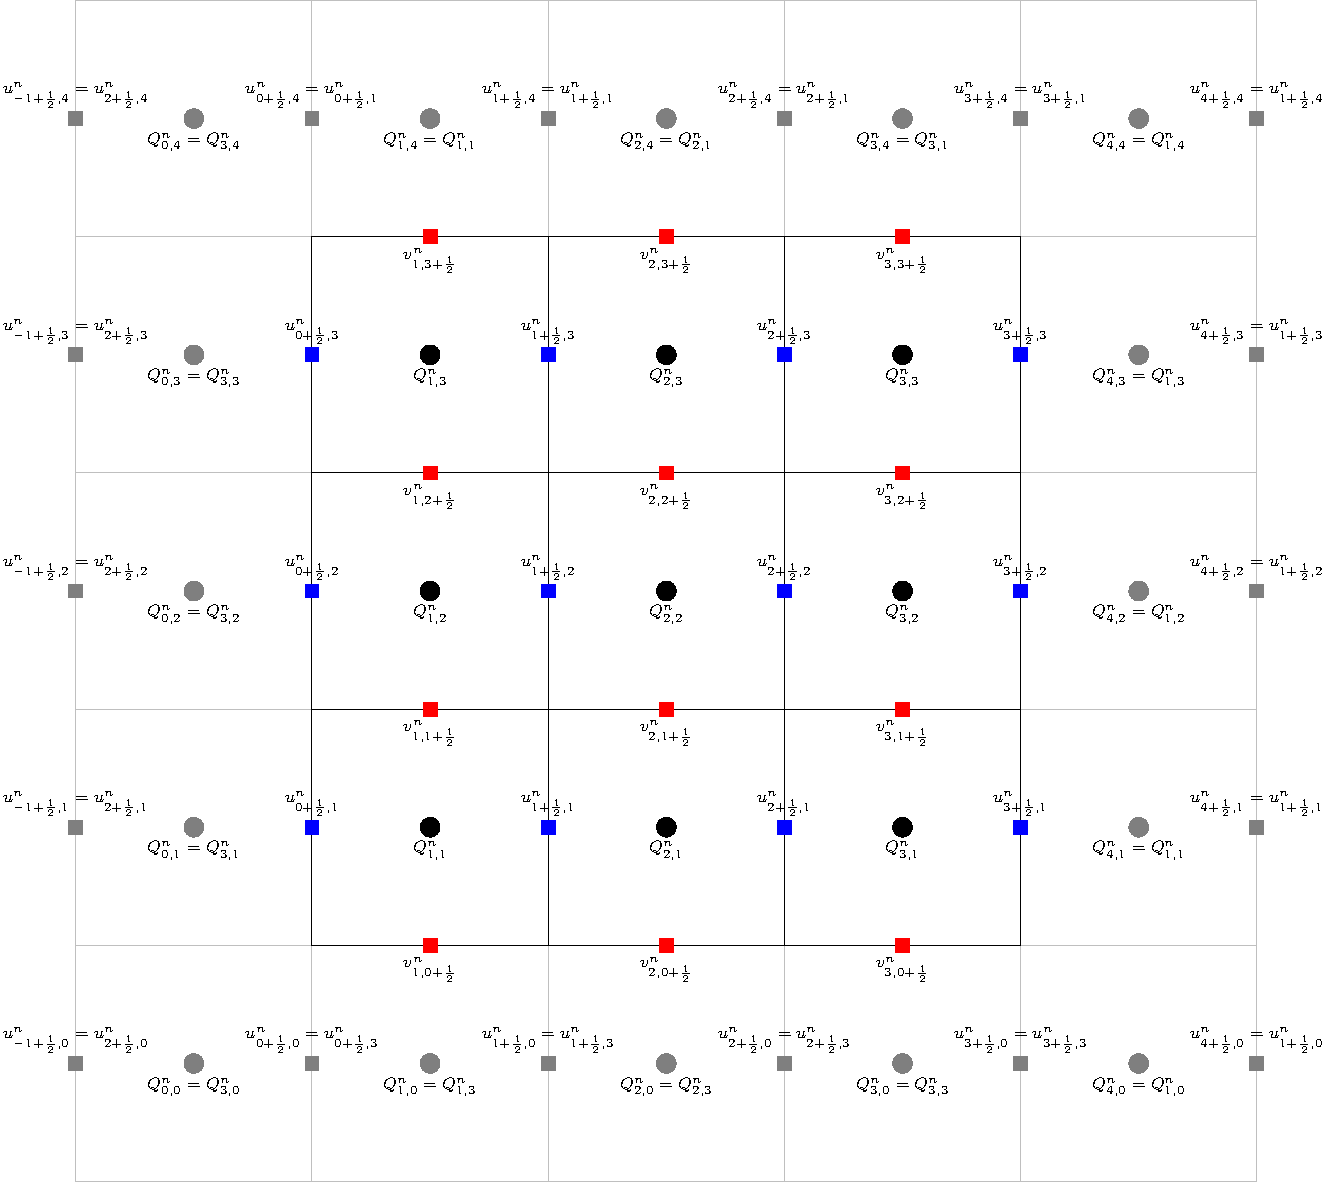
\includegraphics[width=1\linewidth]{2d_grid_function}
	\caption{Illustration of $(\Delta x, \Delta y)$-grid function $Q$ (black circles)
		and a $(\Delta x\Delta y)$-C grid wind $u$ (blue squares) and $v$ (red squares) and its ghost cell
		values (in gray) assuming biperiodicity.\label{chp-adv2d-sec1-grid2d-function}}
\end{figure}

We denote by $\nabla \cdot (q\boldsymbol{u})$ the divergence operator:
\begin{equation}
	\label{sec-adv2d:eqdiv}
	\nabla \cdot (q\boldsymbol{u})(x, y, t) =  
	[{\partial_x (uq)} + {\partial_y (vq)}](x, y, t).
\end{equation}
We recall that we say the $\boldsymbol{u}$ is \textbf{non-divergent} or \textbf{divergent free}  if $\nabla \cdot \boldsymbol{u}=0$.
We define the $(\Delta x, \Delta y)$-grid function $\mathfrak{D}^n$ as
the exact divergence of $q\boldsymbol{u}$ at the cell centers, namely
\begin{equation}
\label{2d-discrete-div}
\mathfrak{D}^n_{ij} = \nabla \cdot (\boldsymbol{u}q)(x_i,y_j,t^n).
\end{equation}
In this Chapter, our focus also lies on periodic grid functions.
We define a $(\Delta x, \Delta y)$-grid function $Q$ as periodic if it satisfies the following conditions:
\begin{align*}
    Q_{i,j} &= Q_{N+i,j}, \quad i=-\nu+1, \ldots, 0,  \quad &j = -\nu+1, \ldots, M+\nu,\\
    Q_{i,j} &= Q_{i-N,j}, \quad i=N+1, \ldots, N+\nu, \quad &j = -\nu+1, \ldots, M+\nu,\\
    Q_{i,j} &= Q_{i,M+j}, \quad j=-\nu+1, \ldots, 0,  \quad &i = -\nu+1, \ldots, N+\nu,\\
    Q_{i,j} &= Q_{i,j-M}, \quad j=M+1, \ldots, M+\nu, \quad &i = -\nu+1, \ldots, N+\nu.
\end{align*}
We use the notation $\mathbb{P}^{N \times M}_{\nu}$ represent the spaces of periodic $(\Delta x, \Delta y)$-grid functions.
Similarly, we define a $(\Delta x, \Delta y)$-grid wind $(u,v)$ as periodic if it meets the following requirements:
\begin{align*}
    u_{i-\frac{1}{2},j} &= u_{N+i+\frac{1}{2},j} , \quad i=-\nu, \ldots, -1,   \quad &j = -\nu+1, \ldots, M+\nu,\\
    u_{i+\frac{1}{2},j} &= u_{i+\frac{1}{2}-N,j} , \quad i=N+1, \ldots, N+\nu, \quad &j = -\nu+1, \ldots, M+\nu,\\
    u_{i+\frac{1}{2},j} &= u_{i+\frac{1}{2},M+j} , \quad i=-\nu, \ldots, N+1+\nu,   \quad &j = -\nu+1, \ldots, 0,\\
    u_{i+\frac{1}{2},j} &= u_{i+\frac{1}{2},j-M} , \quad i=-\nu, \ldots, N+1+\nu,   \quad &j = M+1, \ldots, M+\nu,\\
    v_{i,j-\frac{1}{2}} &= v_{i,M+j+\frac{1}{2}} , \quad j=-\nu, \ldots, -1,   \quad &i = -\nu+1, \ldots, N+\nu,\\
    v_{i,j+\frac{1}{2}} &= v_{i,j+\frac{1}{2}-M} , \quad j=M+1, \ldots, M+\nu, \quad &i = -\nu+1, \ldots, N+\nu,\\
    v_{i,j+\frac{1}{2}} &= v_{N+i,j+\frac{1}{2}} , \quad j=-\nu, \ldots, M+1+\nu,   \quad &i = -\nu+1, \ldots, 0,\\
    v_{i,j+\frac{1}{2}} &= c_{i-N,j+\frac{1}{2}} , \quad j=-\nu, \ldots, N+1+\nu,   \quad &i = N+1, \ldots, N+\nu.\\
\end{align*}
In this case, we use the notation $u \in \mathbb{P}^{(N+1) \times M}_{\nu}$, 
$v \in \mathbb{P}^{N \times (M+1)}_{\nu}$.

For a grid function $Q$ we also use the notations:
\begin{align*}
Q_{\times,j} &:= (Q_{-\nu+1,j}, \ldots, Q_{N+\nu,j}) \in \mathbb{R}^N_{\nu},\\
Q_{i,\times} &:= (Q_{i,-\nu+1}, \ldots, Q_{i,M+\nu}) \in \mathbb{R}^M_{\nu}.
\end{align*}
Given $Q = (Q_{ij})\in \mathbb{P}^{N \times M}_{\nu, P}$, we define the $p$-norm by
\begin{equation}
	\label{chp-adv2d-pnorm}
	\|Q\|_{p,\Delta x \times \Delta y}=
	\begin{cases}
		\bigg( \sum_{i=1}^{N} \sum_{j=1}^{M}|Q_{ij}|^p \bigg)^{\frac{1}{p}} & \text{if } 1\leq p < \infty,\\
		\max_{i=1, \ldots, N,j=1,\ldots,M}{|Q_{ij}|} & \text{if } p=\infty.
	\end{cases}
\end{equation}
We also introduce the centered difference notation:
\begin{align}
	\label{sec-adv2d:eq6}
	\delta_x {h}(x_i,y, t) = 
	{h}(x_{i+\frac{1}{2}}, y, t) - 
	{h}(x_{i-\frac{1}{2}}, y, t), \\
	\delta_y {h}(x, y_j,t) = 
    {h}(x, y_{j+\frac{1}{2}},t) - 
    {h}(x, y_{j-\frac{1}{2}},t),
\end{align}
for any function $h: \Omega \times [0,T] \to \mathbb{R}$.
Additionally, we introduce the average value of $q$ in the control volume
$\Omega_{ij}$ at time $t$, denoted as ${Q}_{ij}(t)$, defined by:
\begin{equation}
	\label{chp-adv2d-sec1-not2}
	{Q}_{ij}(t) = \frac{1}{\Delta x \Delta y}
	\int_{x_{i-\frac{1}{2}}}^{x_{i+\frac{1}{2}}} \int_{y_{j-\frac{1}{2}}}^{y_{j+\frac{1}{2}}} {q}(x,y,t) \,dx.
\end{equation}
Moreover, we define the $(\Delta x, \Delta y)$-grid function of average values as $Q(t) = (Q_{ij}(t))_{i=-\nu+1,\ldots,N+\nu}^{j=-\nu+1,\ldots,M+\nu}$.

For the consideration of periodic boundary conditions, we can define spaces of periodic functions over 
the interval $\Omega$ as follows:
\begin{align*}
	\mathcal{S}_P(\Omega) &= \{q:\mathbb{R}^2\times[0,+\infty[\to \mathbb{R}: q(x+b-a,y+d-c,t)=q(x,y,t), \quad \forall x,y \in \mathbb{R}, \quad t\geq0\}.
\end{align*}
Similarly, the space of $k$-times periodically differentiable functions $\mathcal{C}_P^k(\Omega)$ can be defined as:
\begin{align*}
	\mathcal{C}_P^k(\Omega) &= \mathcal{S}_P(\Omega) \cap \mathcal{C}^k(\mathbb{R}^2\times[0,\infty[),
\end{align*}
where $\mathcal{C}^k(\mathbb{R}^2\times[0,+\infty[)$ denotes the space of functions that are $k$ 
times continuously differentiable in both the spatial and temporal variables.
In summary, $\mathcal{S}_P(\Omega)$ represents the space of periodic functions, and $\mathcal{C}_P^k(\Omega)$
represents the space of $k$-times periodically differentiable functions over $\Omega$ subject to periodic boundary conditions.

\subsection{The 2D advection equation}
\label{chp-adv2d-sec1}
Let us consider a  velocity field given by $\boldsymbol{u}=(u,v)$, where
$u$ is the velocity in $x$-direction and $v$ is the velocity in $x$ and $y$ direction
and $u,v \in \mathcal{C}^1_P(\Omega)$.
The two-dimensional advection equation in its differential form in 
a domain $\Omega$ associated to the velocity field or wind $\boldsymbol{u}$ 
and assuming biperiodic boundary conditions is given by:
\begin{equation}
	\label{sec-adv2d:eq1}
	\begin{cases}
		[{\partial_t q} + {\partial_x (uq)} +  {\partial_y (vq)}](x, y, t)
		= 0, \quad \forall (x,y,t) \in \mathbb{R}^2\times ]0, +\infty[,\\
		{q}(a, y, t) = {q}(b, y, t), \quad \forall y \in [c,d],  \quad \forall t\geq 0, \\
		{q}(x, c, t) = {q}(x, d, t), \quad \forall x \in [a,b],  \quad \forall t\geq 0, \\
		q_0(x) = q(x,y,0), \quad \forall (x,y) \in \Omega.
	\end{cases}
\end{equation} 
A classical or strong solution to the two-dimensional advection equation is a 
$\mathcal{C}^1_P{(\Omega)}$ function ${q}$ satisfying Equation \eqref{sec-adv2d:eq1}.
As we did in Section \ref{chp-adv1d-sec1}, our goal is to deduce an
integral form of Equation \eqref{sec-adv2d:eq1}.
Thus, let us consider  $[x_1,x_2] \times [y_1, y_2]
\subset \Omega$ and $[t_1,t_2] \subset [0, +\infty[$.
Integrating Equation $\eqref{sec-adv2d:eq1}$ over 
$[x_1,x_2] \times [y_1, y_2]$ yields:
\begin{align}
	\label{sec-adv2d:eq2}
	\frac{d}{d t} \bigg(\int_{x_1}^{x_2} \int_{y_1}^{y_2}
	{q}(x, y, t) \,dx \,dy \bigg)=
	&-\int_{y_1}^{y_2} \bigg({(uq)}(x_2, y, t)
	-{(uq)}(x_1, y, t) \bigg) \,dy \\ \nonumber
	&-\int_{x_1}^{x_2} \bigg({(vq)}(x, y_2, t)
	-{(vq)}(x, y_1, t) \bigg) \,dx.
\end{align}
Integrating Equation \eqref{sec-adv2d:eq2} over the time interval $[t_1,t_2]$, 
we have:
\begin{align}
	\label{sec-adv2d:eq3}
	\int_{x_1}^{x_2} \int_{y_1}^{y_2}
	{q}(x, y, t_{n+1}) \,dx \,dy = &\int_{x_1}^{x_2} \int_{y_1}^{y_2}
	{q}(x, y, t_n) \,dx \,dy \\ \nonumber
	&-\int_{t_1}^{t_2} \int_{y_1}^{y_2} \bigg({(uq)}(x_2, y, t)
	-{(uq)}(x_1, y, t) \bigg) \,dy \,dt\\ \nonumber
	&-\int_{t_1}^{t_2} \int_{x_1}^{x_2} \bigg({(vq)}(x, y_2, t)
	-{(vq)}(x, y_1, t) \bigg) \,dx \,dt.
\end{align}
Equation \eqref{sec-adv2d:eq3} is the integral form of Equation 
\eqref{sec-adv2d:eq1}. We say that ${q}$ is a weak
solution to the advection equation \eqref{sec-adv2d:eq1} if ${q}$
satisfies the integral form \eqref{sec-adv2d:eq3}, 
$\forall [x_1,x_2]\times[y_1,y_2] \subset \Omega^{\mathrm{o}}$ and 
$\forall [t_1,t_2] \subset [0,+\infty[$.
We summarize the weak version of Equation \eqref{sec-adv2d:eq1} in Problem \eqref{chp-adv2d-sec2-prob1}.
\begin{prob}
	\label{chp-adv2d-sec2-prob1}
	Given an initial condition ${q}_0$ and
	a velocity function $\boldsymbol{u} = (u,v)$
 	we would like to find a weak solution ${q}$
	of the two-dimensional advection equation in its integral form:
	\begin{align*}
		\int_{x_1}^{x_2} \int_{y_1}^{y_2}
		{q}(x, y, t) \,dx \,dy = &\int_{x_1}^{x_2} \int_{y_1}^{y_2}
		{q}(x, y, t) \,dx \,dy \\ \nonumber
		&-\int_{t_1}^{t_2} \int_{y_1}^{y_2} \bigg({(uq)}(x_2, y, t)
		-{(uq)}(x_1, y, t) \bigg) \,dy \,dt\\ \nonumber
		&-\int_{t_1}^{t_2} \int_{x_1}^{x_2} \bigg({(vq)}(x, y_2, t)
		-{(vq)}(x, y_1, t) \bigg) \,dx \,dt.
	\end{align*}
	$\forall [x_1, x_2]\times [y_1, y_2] \times[t_1, t_2] \subset \Omega \times[0,T]$, 
	and ${q}(x, y, 0) = {q}_0(x, y)$, $\forall (x, y) \in \Omega$,
   ${q}(a, y, t) = {q}(b, y, t), \quad \forall y \in [c,d],  \quad \forall t\geq 0,$
   ${q}(x, c, t) = {q}(x, d, t), \quad \forall x \in [a,b],  \quad \forall t\geq 0.$
\end{prob}
Similarly to Section \ref{chp-adv1d-sec1}, Equation \eqref{sec-adv2d:eq1} and Problem \eqref{chp-adv2d-sec2-prob1} are equivalent
when ${q}, \boldsymbol{u} \in \mathcal{C}^1_P{(\Omega)}$.
For Problem \ref{chp-adv2d-sec2-prob1}, the total mass in $\Omega$ is defined by: 
\begin{equation}
	{M}_{\Omega}(t) = \int_{\Omega} {q}(x,y,t) \,dx \,dy , \quad \forall t \in [0,T],
\end{equation}
and is conserved within time: 
\begin{equation}
	{M}_{\Omega}(t) = {M}_{\Omega}(0), \quad \forall t \in [0,T].
\end{equation}
Considering a $(\Delta x, \Delta y, \Delta t, \lambda)$ discretization of $D = \Omega \times [0,T]$ and
substituting $t_1, t_2, x_1, x_2, y_1$ and $y_2$ by 
$t_{n}, t_{n+1}, x_{i-\frac{1}{2}}, x_{i+\frac{1}{2}}, y_{j-\frac{1}{2}}, y_{j+\frac{1}{2}}$,
respectively, in Equation \eqref{sec-adv2d:eq3}, we obtain:
\begin{align}
	\label{sec-adv2d:eq5}
	{Q}_{ij}(t_{n+1})  = {Q}_{ij}(t_{n})
	&- \frac{\Delta t}{\Delta x \Delta y}
	\delta _x \bigg( \frac{1}{\Delta t}
	\int_{t_1}^{t_2} \int_{y_{j-\frac{1}{2}}}^{y_{j+\frac{1}{2}}} 
	{(uq)}(x_{i}, y, t)
	\,dy \,dt \bigg) \\ \nonumber
	&- \frac{\Delta t}{\Delta x \Delta y}
	\delta _y \bigg( \frac{1}{\Delta t}
	\int_{t_1}^{t_2} \int_{x_{i-\frac{1}{2}}}^{x_{i+\frac{1}{2}}} 
	{(vq)}(x, y_{j}, t)
	\,dx \,dt \bigg),
\end{align}
where we are using the centered finite-difference notation.
Now we can define a discretized version of Problem \ref{chp-adv2d-sec2-prob1} as Problem \ref{chp-adv2d-sec2-prob2}.
\begin{prob}
	\label{chp-adv2d-sec2-prob2}
	Assume the framework of Problem \ref{chp-adv2d-sec2-prob1}
	and consider a $(\Delta x, \Delta y, \Delta t, \lambda)$-discretization of $\Omega\times [0,T]$.
	Since we are in the framework of Problem \ref{chp-adv2d-sec2-prob1}, it follows that:
	\begin{align*}
		{Q}_{ij}(t_{n+1})  = {Q}_{ij}(t_{n})
		&- {\lambda}
		\delta _x \bigg( \frac{1}{\Delta t \Delta y}
		\int_{t^n}^{t^{n+1}} \int_{y_{j-\frac{1}{2}}}^{y_{j+\frac{1}{2}}} 
		{(uq)}(x_{i}, y, t)
		\,dy \,dt \bigg) \\ \nonumber
		&- {\lambda}
		\delta _y \bigg( \frac{1}{\Delta t \Delta x}
		\int_{t^n}^{t^{n+1}} \int_{x_{i-\frac{1}{2}}}^{x_{i+\frac{1}{2}}} 
		{(vq)}(x, y_{j}, t)
		\,dx \,dt \bigg),
	\end{align*}
	where ${Q}_{ij}(t) = \frac{1}{\Delta x \Delta y}
	\int_{x_{i-\frac{1}{2}}}^{x_{i+\frac{1}{2}}} 
	\int_{y_{j-\frac{1}{2}}}^{y_{j+\frac{1}{2}}} {q}(x,y,t) \,dx \,dy$.
	Our problem now consists of finding the values ${Q}_{ij}(t_{n})$, 
	$\forall i = 1, \ldots, N$, $\forall j = 1, \ldots, M$, $\forall n = 0, \ldots, N_T-1$,
    given the initial values ${Q}_{ij}(0)$, $\forall i = 1, \ldots N$, $\forall j = 1, \ldots, M$.
    In other words, we aim to find the average values of ${q}$ in each control volume $\Omega_{ij}$ at the specified time instances.
\end{prob}
It is important to note that no approximations have been made in Problems \eqref{chp-adv2d-sec2-prob1} and \eqref{chp-adv2d-sec2-prob2}. 

\section{The finite-volume approach}
\label{sec:fv-2d}
Finally, we define the 2D-FV scheme problem as follows in Problem \ref{chp-adv2d-sec2-prob3}.
\begin{prob}[2D-FV scheme]
	\label{chp-adv2d-sec2-prob3}
	Assume the framework defined in Problem \ref{chp-adv2d-sec2-prob2}.
	The finite-volume approach of Problem \ref{chp-adv2d-sec2-prob2}
	consists of a finding a scheme of the form:
	\begin{align}
		\label{chp-adv2d-2dfv}
		{Q}_{ij}^{n+1} =  {Q}_{ij}^{n} - {\lambda} \delta_i {F}_{ij}^{n} - {\lambda} \delta_j {G}_{ij}^{n},
		\\ \nonumber \quad \forall i = 1, \ldots, N, \quad \forall j = 1, \ldots, M,
		\quad \forall n = 0, \ldots, N_T-1,
	\end{align}
	where $ \delta_i F_{ij}^n =
    {F}_{i+\frac{1}{2},j}^{n} 
    - {F}_{i-\frac{1}{2},j}^{n}$,
    $ \delta_j G_{ij}^n =
    {G}_{i,j+\frac{1}{2}}^{n} 
    - {G}_{i,j-\frac{1}{2}}^{n}$ 
    and ${Q}^{n}\in \mathbb{P}^{N\times M}_{\nu}$ is intended to be an approximation
	of ${Q}(t_{n})\in \mathbb{P}^{N\times M}_{\nu}$ in some sense. We define ${Q}_{ij}^{0} = {Q}_{ij}(0)$ or
	${Q}_{ij}^{0} = {q}^0_{ij}$.
    
    The term ${F}_{i+\frac{1}{2}, j}^{n}$ is known as numerical flux in the 
    $x$ direction and it approximates
	$\frac{1}{\Delta t \Delta y}\int_{t_n}^{t_{n+1}} 
    \int_{y_{j-\frac{1}{2}}}^{y_{j+\frac{1}{2}}} 
    (uq)(x_{i+\frac{1}{2}}, y, t) \,dy \,dt $,
    $\forall i = 0, 1, \ldots, N$, and 
	${G}_{i, j+\frac{1}{2}}^{n}$ is known as numerical flux in the 
    $y$ direction and it approximates
	$\frac{1}{\Delta t \Delta x}\int_{t_n}^{t_{n+1}}  
    \int_{x_{i-\frac{1}{2}}}^{x_{i+\frac{1}{2}}}
    (vq)(x, y_{j+\frac{1}{2}}, t) \,dx \,dt $,
    $\forall j = 0, 1, \ldots, M$,
	or, in other words, they estimate the time-averaged
    fluxes at the control volume $\Omega_{ij}$ boundaries.
\end{prob}
\begin{remark}
For Problem \ref{chp-adv2d-sec2-prob3}, we define the CFL number in the $x$ and $y$ direction
by $\max_{i,j} \{{|u_{i+\frac{1}{2},j}^n}|\}\frac{\Delta t}{\Delta x}$ and 
$\max_{i,j} \{ {|v_{i,j+\frac{1}{2}}^n}|\}\frac{\Delta t}{\Delta y}$, respectively.
The CFL number is maximum between these numbers and we say that the CFL condition is
satisfied if the CFL number is less than one. 
\end{remark}
For a 2D-FV the discrete total mass at the time-step $n$ is given by
\begin{equation*}
	M^n =  \Delta x \Delta y \sum_{i=1}^N \sum_{j=1}^M Q_{ij}^n.
\end{equation*}
Therefore, the discrete total mass is constant for a 2D-FV scheme,
which follows from a straightforward computation:
\begin{align*}
	M^{n+1} &=  \Delta x \sum_{i=1}^N  \sum_{j=1}^M Q_{ij}^{n+1} 
	= M^{n} - \Delta t  \sum_{i=1}^N  \sum_{j=1}^M (F^n_{i+\frac{1}{2},j}- F^n_{i-\frac{1}{2},j})
	 		 - \Delta t  \sum_{i=1}^N  \sum_{j=1}^M (G^n_{i,j+\frac{1}{2}}- G^n_{i,j-\frac{1}{2}})\\
	&= M^{n} - \Delta t \sum_{j=1}^M (F^n_{N+\frac{1}{2},j}- F^n_{\frac{1}{2},j})
			 - \Delta t \sum_{i=1}^N (G^n_{i,M+\frac{1}{2}}- G^n_{i,\frac{1}{2}})
	= M^{n},
\end{align*}
where we are using that $F^n_{N+\frac{1}{2},j} = F^n_{\frac{1}{2},j}$,
$G^n_{i,M+\frac{1}{2}} = G^n_{i,\frac{1}{2}}$ since we are assuming bi-periodic boundary
conditions.

As we mentioned in Problem \ref{chp-adv2d-sec2-prob3}, the initial condition may be assumed as $q_{ij}^0$ or $Q_{ij}(0)$. 
For two-dimensional simulations, we are going to assume  $q_{ij}^0$ as initial data to avoid the computation of integrals.
Furthermore, the errors will be calculated using the values $q_{ij}^n$ instead of $Q_{ij}(t_n)$.
Similarly to Proposition \ref{prop-bound-centroid}, we have that the centroid value approximates the average value
with second order, as Proposition \ref{prop-bound-centroid-2d} shows.
\begin{prop}
	\label{prop-bound-centroid-2d}
	If $q \in \mathcal{C}^2$, then $|Q_{ij}(t^n)-q_{ij}^n| = C_1 \Delta x^2 + C_2 \Delta x \Delta y + C_3 \Delta y^2$, where 
	$C_1$, $C_2$ and $C_3$ are constants.
\end{prop}
\begin{proof}
	Just apply Theorem \ref{prop-bound-midpoint2d} for the function $q(x,y,t^n)$.	
\end{proof}

In order to check the consistency of 2D-FV, it is useful to use the notion of discrete divergence.
\begin{definition}[Discrete divergence]
	\label{chp-adv2d-def-div}
	For Problem \ref{chp-adv2d-sec2-prob3}, we define the discrete divergence as a 
    $(\Delta x, \Delta y)$-grid function $\mathbb{D}^n(Q^n,u^n,v^n) \in \mathbb{P}^{N\times M}_{\nu}$
	given by:
	\begin{equation}
		\label{chp-adv2d-def-div-eq}
		\mathbb{D}_{ij}^n(Q^n,u^n,v^n)=  \frac{1}{\Delta t}
        \bigg(\frac{\delta_i {F}_{ij}^{n}}{\Delta x} + \frac{\delta_j {G}_{ij}^{n}}{\Delta y} \bigg), 
        \quad i = 1, \ldots, N, \quad j=1, \ldots,M.
	\end{equation}
\end{definition}
With the aid of the discrete divergence, we may rewrite Equation \eqref{chp-adv2d-2dfv} as:
\begin{align}
    \label{chp-adv2d-2dfv-div}
    {Q}^{n+1} =  {Q}^{n} - \Delta t \mathbb{D}^n(Q^n,u^n,v^n),
\end{align}
Notice that if we replace  $Q^n$ by the exact solution $Q(t^n)$ in Equation \eqref{chp-adv2d-2dfv-div}, we have
\begin{align}
    \label{chp-adv2d-div-tau}
    {Q}(t^{n+1}) =  {Q}(t^{n}) - \Delta t \mathbb{D}^n(Q(t^n),u^n,v^n) - \Delta t \tau^n,
\end{align}
where $\tau^n \in \mathbb{P}^{N\times M}_{\nu}$ is the local truncation error (LTE).
Rearranging the terms of Equation \eqref{chp-adv2d-div-tau}, we obtain:
\begin{align}
    \label{chp-adv2d-div-tau2}
    \tau^n =  \frac{{Q}(t^{n+1}) - {Q}(t^{n})}{\Delta t} - \mathbb{D}^n(Q(t^n),u^n,v^n).
\end{align}
We define the consistency of the 2D-FV scheme as follows.
\begin{definition}[Consistency]
	\label{chp-adv2d-def-cons}
	Let us consider the framework of Problem \ref{chp-adv2d-sec2-prob3}.
	A 2D-FV scheme is said to be consist in the $p$-norm if for any sequence of
	$(\Delta x^{(k)},\Delta y^{(k)}, \Delta t^{(k)},\lambda)$-discretizations, 
	$k \in \mathbb{N}$, with
    $\lim_{k\to \infty }{\Delta x^{(k)}} =\lim_{k\to \infty }{\Delta y^{(k)}}= \lim_{k\to \infty }{\Delta t^{(k)}} = 0$, we have:
	\begin{equation*}
		\lim_{k \to \infty}\bigg[ {\max_{1\leq n\leq N_T^{(k)}}}{\|\tau^n\|_{p,\Delta x^{(k)} \times \Delta y^{(k)}}} \bigg] = 0,
	\end{equation*}
	and it is said to be consistent with order $d$ in the $p-$norm if
	\begin{equation*}
		{\max_{1\leq n\leq N_T^{(k)}}}{\|\tau^n\|_{p,\Delta x^{(k)} \times \Delta y^{(k)}}} = \mathcal{O}(\Delta x^d).
	\end{equation*}
\end{definition}
The relationship between consistency and convergence is explained in Section \ref{chp-adv2d-CCS}.
If $q$ satisfies Equation \eqref{sec-adv2d:eq1}, it can be observed that consistency is equivalent to the following:
\begin{equation*}
	{\max_{1\leq n\leq N_T^{(k)}}}{\|\mathfrak{D}^n - \mathbb{D}^n(Q^n,u^n,v^n)\|_{p,\Delta x^{(k)} \times \Delta y^{(k)}}} = \mathcal{O}(\Delta x^d),
\end{equation*}
where $\mathfrak{D}^n \in \mathbb{P}^{N\times M}_{\nu}$ is defined in Equation \eqref{2d-discrete-div}.
Therefore, we can determine whether a 2D-FV scheme is consistent by comparing the discrete divergence to the exact divergence.

\section{Dimension splitting}
\label{sec-dsplit}
This Section aims to demonstrate how a 2D-FV scheme, such as the one presented in Problem \ref{chp-adv2d-sec2-prob3},
can be constructed using 1D-FV schemes through a technique known as dimension splitting.
Before introducing the dimension splitting scheme proposed by \citet{lin:1996},
it is helpful to examine general operator splitting schemes,
as the dimension splitting technique is a specific instance of operator splitting methods.

For a given time interval $[0,T]$, we utilize a $\Delta t$-temporal grid. Let us consider the abstract Cauchy problem.
\begin{align*}
	\begin{cases}
		\frac{dq}{dt}(t) &= Aq(t), \quad t \in [t^n,t^{n+1}],\\
		q(t^n) &= q_n,
	\end{cases}
\end{align*}
for $n=0,\ldots, N_T-1$, where $q(t) \in \mathcal{B}$ for some Banach space $\mathcal{B}$, and $A:\mathcal{B} \to \mathcal{B}$ is a linear operator
following the framework of \citet[Chapter~3]{richtmyer:1968}.
We are interested in finding $q(t^{n+1})$ given $q_n$.
Assuming that $A = A_1 + A_2$ for two linear operators $A_1, A_2:\mathcal{B} \to \mathcal{B}$, we consider the following abstract Cauchy sub-problems:
\begin{align*}
	\begin{cases}
		\frac{dq^1}{dt}(t) &= A_1q(t), \quad t \in [t^{n},t^{n+1}],\\
		q^{1}(t^n) &= q_n,
	\end{cases}
\end{align*}
and
\begin{align*}
	\begin{cases}
		\frac{dq^{21}}{dt}(t) &= A_2q(t), \quad t \in [t^n,t^{n+1}],\\
		q^{21}(t^n) &= q^1(t^{n+1}).
	\end{cases}
\end{align*}
Then we can approximate $q(t_0 + \Delta t)$ as $q^{21}(t^n + \Delta t)$ 
with an error of $\mathcal{O}(\Delta t)$ if $A_1$ and $A_2$ do not commute. 
Otherwise, this method is exact.
This approach is known as Lie-Trotter splitting. 
It's worth noting that the Lie-Trotter splitting can also be performed in reverse order when solving the sub-problems:
\begin{align*}
	\begin{cases}
		\frac{dq^2}{dt}(t) &= A_2q(t), \quad t \in [t^n,t^{n+1}],\\
		q^{2}(t^n) &= q_n,
	\end{cases}
\end{align*}
and 
\begin{align*}
	\begin{cases}
		\frac{dq^{21}}{dt}(t) &= A_1q(t), \quad t \in [t^n,t^{n+1}],\\
		q^{12}(t^n) &= q^1(t^{n+1}),
	\end{cases}
\end{align*}
and again we estimate $q(t^{n+1})$ by $q^{12}(t^{n+1})$ with error $\mathcal{O}(\Delta t)$.
As noted by \citet{strang:1968}, we can consider the following equation 
to approximate $q(t^{n+1})$ using a second-order ($\mathcal{O}(\Delta t^2)$) symmetric scheme:
\begin{equation}
	q^*(t^{n+1}) = \frac{q^{21}(t^{n+1}) + q^{12}(t^{n+1})}{2},
\end{equation}
This scheme is referred to as the average Lie-Trotter splitting \citep{holden:2010}.
The process of averaging two Lie-Trotter splittings is a specific case of methods
known as weighted sequential splitting methods in the literature.
Furthermore, this scheme averaging process can be extended to achieve higher-order schemes \citep{jia:2011}.
For an analysis of the accuracy of weighted sequential splitting methods, we recommend referring to \citet{csomos:2005}.


It is worth noting that one of the most commonly used second-order splitting schemes in the literature is the Strang splitting
\citep{strang:1968}.
This scheme requires solving three sub-problems per time-step, with one of them at time $t_n + \frac{\Delta t}{2}$.
In contrast, the average Lie-Trotter splitting requires solving four sub-problems per time-step.
Consequently, the Strang splitting is computationally more efficient.
However, as we will observe in this Chapter, when applied to the linear advection equation, 
the average Lie-Trotter splitting allows for a modification that eliminates a splitting error
arising from considering a constant scalar field and non-divergent velocity \citep{lin:1996}.

\subsection{Lie-Trotter splitting using PPM}
\label{lit-trotter-sp}
To move towards the scheme from \citet{lin:1996}, let us consider Problem \ref{chp-adv2d-sec2-prob1} in its differential form (Equation \eqref{sec-adv2d:eq1}).
We are going to consider $N+2\nu$ one-dimensional advection equations in the $x$-direction:
\begin{equation*}
	\label{chp-adv2d-adv2deq-xdir1}
	[{\partial_t q^x}+{\partial_x (uq^x)}](x, y_j, t)
	= 0,
\end{equation*}
for $j=-\nu+1, \ldots, M+\nu$,
and the $N+2\nu$ one-dimensional advection equations in the $y$-direction
\begin{equation*}
	\label{chp-adv2d-adv2deq-ydir1}
	[{\partial_t q^y} +{\partial_y (vq^y)}](x_i, y, t) = 0,
\end{equation*}
for, $i=-\nu+1, \ldots, N+\nu$.

We shall assume that these problems are solved using a 1D-FV scheme as in Problem \ref{chp-adv1d-sec2-prob4}
with the PPM numerical flux functions $\mathfrak{F}_{i+\frac{1}{2},j}^{PPM,x}[Q^n_{\times,j},\tilde{c}^{x,n}]$ and
$\mathfrak{F}_{i,j+\frac{1}{2}}^{PPM,y}[Q^n_{i,\times},\tilde{c}^{y,n}]$, respectively,
where $\tilde{c}^{x,n}_{i+\frac{1}{2},j}$ is the time-averaged CFL used in the departure point estimation in the $x$ direction
and $\tilde{c}^{y,n}_{i,j+\frac{1}{2}}$ is the time-averaged CFL used in the departure point estimation in the $y$ direction,
assuming that the CFL number is less than one (see Equation \eqref{chp-sec-flux:numerical-flux8}).
The time-averaged CFL numbers are computed using the schemes 
\textbf{DP1} (Subsection \ref{chp-adv1d-sec-DP1}) and \textbf{DP2}
(Subsection \ref{chp-adv1d-sec-DP2}), applied separately in the $x$ and $y$ directions.

The values $q_{L,ij}^x$, $q_{R,ij}^x$, $q_{L,ij}^y$, and $q_{R,ij}^y$,
which approximate values of $q$, namely 
$q_{i-\frac{1}{2},j}$, $q_{i+\frac{1}{2},j}$, $q_{i,j-\frac{1}{2}}$, $q_{i,j+\frac{1}{2}}$, respectively,
are computed using one of the schemes unlimited PPM ({hord0}) and limited PPM ({hord8}) as described
in Sections \ref{chp-adv1d-sec-hord0} and \ref{chp-adv1d-sec-hord8}, again
applied separately in the $x$ and $y$ directions.
These approximations are expected to be
second-order accurate because the given average values are computed on the
2D control volume $\Omega_{ij}$ instead of the 1D control volumes $X_i$ or $Y_j$.

As in Section \ref{chp-adv1d-sec-flux}, 
in Equations \eqref{chp-sec-flux:numerical-flux6} and \eqref{chp-sec-flux:numerical-flux6}, 
we define the perturbation values in the $x$ direction as:
\begin{align}
\label{chp-adv2d-pertb-xL}
b_{L,i,j}^x &= q_{L,i,j}^x - Q_{ij}^n, \\
\label{chp-adv2d-pertb-xR}
b_{R,i,j}^x &= q_{R,i,j}^x - Q_{ij}^n,
\end{align}
and the perturbation values in the $y$ direction as:
\begin{align}
\label{chp-adv2d-pertb-yL}
b_{L,i,j}^y &= q_{L,i,j}^y - Q_{ij}^n, \\
\label{chp-adv2d-pertb-yR}
b_{R,i,j}^y &= q_{R,i,j}^y - Q_{ij}^n.
\end{align}
Then, we may express the 1D fluxes in $x$ direction as in Equation \eqref{chp-sec-flux:numerical-flux8}, namely:
\begin{equation}
	\label{chp-adv2d-flux-xdir}
        \mathfrak{F}_{i+\frac{1}{2},j}^{PPM,x}[Q_{\times,j}^n,\tilde{c}^{x,n}]  =  
    	\begin{cases}
        Q_{ij}^n +
        (1-\tilde{c}_{{i+\frac{1}{2},j}}^{x,n})
        \big(b_{R,i,j}^x-\tilde{c}_{{i+\frac{1}{2},j}}^{x,n}
        (b_{L,i,j}^x+b_{R,i,j}^x)\big),
	& \text{if } \tilde{c}_{i+\frac{1}{2},j}^{x,n} \geq 0,\\
	Q_{i+1,j}^n +
        (1+\tilde{c}_{{i+\frac{1}{2},j}}^{x,n})
        \big(b_{L,i+1,j}^x+\tilde{c}_{{i+\frac{1}{2},j}}^{x,n}
        (b_{L,i+1,j}^x+b_{R,i+1,j}^x)\big),
	& \text{if } \tilde{c}_{i+\frac{1}{2},j}^{x,n}<0,
    	\end{cases}
\end{equation}
for $i=0, \ldots, N$, $j=-\nu+1, \ldots, M + \nu$, and the 1D fluxes in $y$ direction reads
\begin{equation}
	\label{chp-adv2d-flux-ydir}
        \mathfrak{F}_{i,j+\frac{1}{2}}^{PPM,y}[Q_{i,\times}^n,\tilde{c}^{y,n}]  =  
    	\begin{cases}
        Q_{ij}^n +
        (1-\tilde{c}_{{i,j+\frac{1}{2}}}^{y,n})
        \big(b_{R,i,j}^y-\tilde{c}_{{i,j+\frac{1}{2}}}^{y,n}
        (b_{L,i,j}^y+b_{R,i,j}^y)\big),
	& \text{if } \tilde{c}_{i,j+\frac{1}{2}}^{y,n} \geq 0,\\
	Q_{i,j+1}^n +
        (1+\tilde{c}_{{i,j+\frac{1}{2}}}^{y,n})
        \big(b_{L,i,j+1}^y+\tilde{c}_{{i,j+\frac{1}{2}}}^{y,n}
        (b_{L,i,j+1}^y+b_{R,i,j+1}^y)\big),
	& \text{if } \tilde{c}_{i,j+\frac{1}{2}}^{y,n}<0,
    	\end{cases}
\end{equation}
for $i=-\nu+1, \ldots, N + \nu$, $j=0, \ldots, M$.
For both the unlimited (hord0) and limited (hord8) PPM schemes, we set $\nu=3$.

We introduce the auxiliary grid functions $\mathbf{F}$ and $\mathbf{G}$, both belonging to $\mathbb{R}^{N\times M}_{\nu}$, given by:
\begin{align*}
\mathbf{F}_{ij}[{Q^n,\tilde{c}^{x,n}}] = 
-\frac{1}{|\Omega_{ij}|}
	  \bigg(\mathcal{A}_{i+\frac{1}{2},j}^{x} \mathfrak{F}_{i+\frac{1}{2},j}^{PPM,x}[Q^n_{\times,j},\tilde{c}^{x,n}]-
               \mathcal{A}_{i-\frac{1}{2},j}^{x} \mathfrak{F}_{i-\frac{1}{2},j}^{PPM,x}[Q^n_{\times,j},\tilde{c}^{x,n}] \bigg),
\end{align*}
for $i=1, \ldots, N$, $j=-\nu+1, \ldots, M + \nu$, and
\begin{align*}
\mathbf{G}_{ij}[{Q^n,\tilde{c}^{y,n}}] = 
-\frac{1}{|\Omega_{ij}|}
	  \bigg(\mathcal{A}_{i,j+\frac{1}{2}}^{y} \mathfrak{F}_{i,j+\frac{1}{2}}^{PPM,y}[Q^n_{i,\times},\tilde{c}^{y,n}]-
                \mathcal{A}_{i,j-\frac{1}{2}}^{y} \mathfrak{F}_{i,j-\frac{1}{2}}^{PPM,y}[Q^n_{i,\times},\tilde{c}^{y,n}] \bigg),
\end{align*}
for $i=-\nu+1, \ldots, N + \nu$  $j=1, \ldots, M$.
We are using the notations $|\Omega_{ij}|= \Delta x \Delta y$ to represent the area of the control volume and
\begin{align*}
\mathcal{A}_{i+\frac{1}{2},j}^{x} = \tilde{c}_{i+\frac{1}{2},j}^{x,n} \Delta x \Delta y,\\
\mathcal{A}_{i,j+\frac{1}{2}}^{y} = \tilde{c}_{i,j+\frac{1}{2}}^{y,n} \Delta x \Delta y.
\end{align*}
This notation shall be useful when we consider these schemes on the cubed-sphere in Chapter \ref{chp-cs-fv}.
Hence, the operators $\mathbf{F}$ and $\mathbf{G}$ represent the numerical updates added to the average values 
at time level $n$ to obtain their values at time level $n+1$ when solving the advection equation in the $x$ and $y$ directions, respectively.

\begin{figure}[!htb]
	\centering
	\begin{subfigure}{0.3\textwidth}
		\centering
		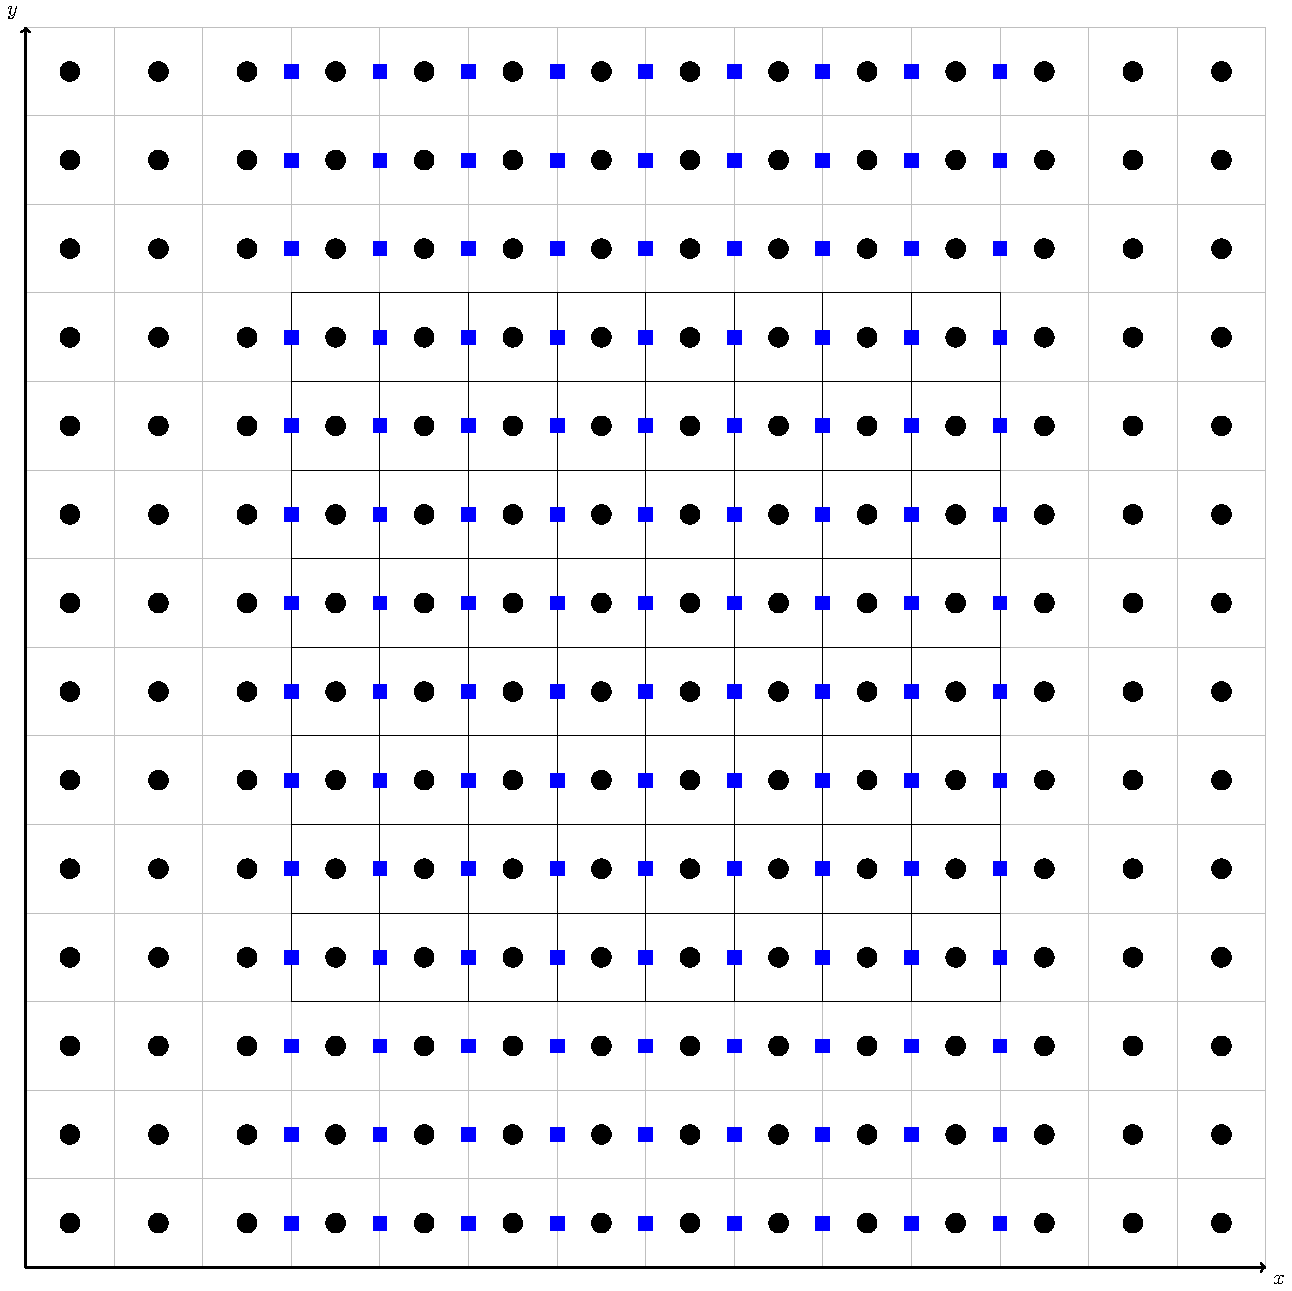
\includegraphics[width=1\linewidth]{2d_grid_Qx}
		\caption{$Q^n$ (black circles) and $u$ at edges (blue squares). \label{lt-Qx}}
	\end{subfigure}
	\begin{subfigure}{0.3\textwidth}
		\centering
		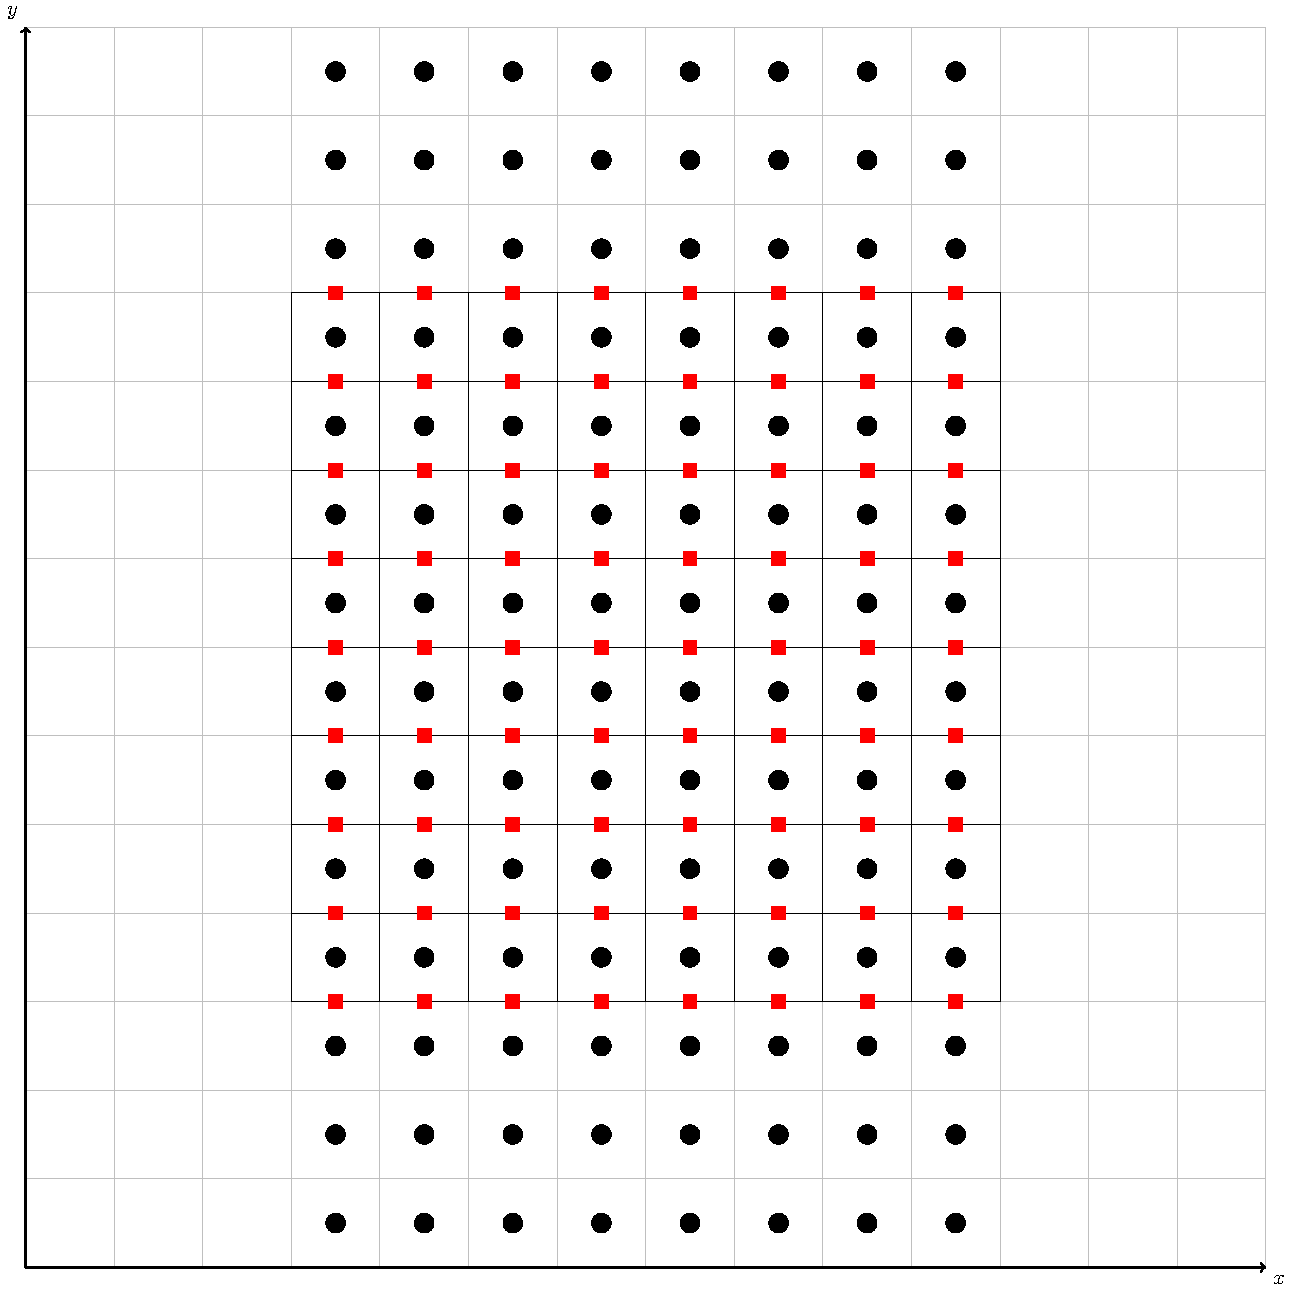
\includegraphics[width=1\linewidth]{2d_grid_FQ}
		\caption{$Q^{x,n}$ (black circles) and $v$ at edges (red squares).\label{lt-FQx} }
	\end{subfigure}
	\begin{subfigure}{0.3\textwidth}
	    \centering
	    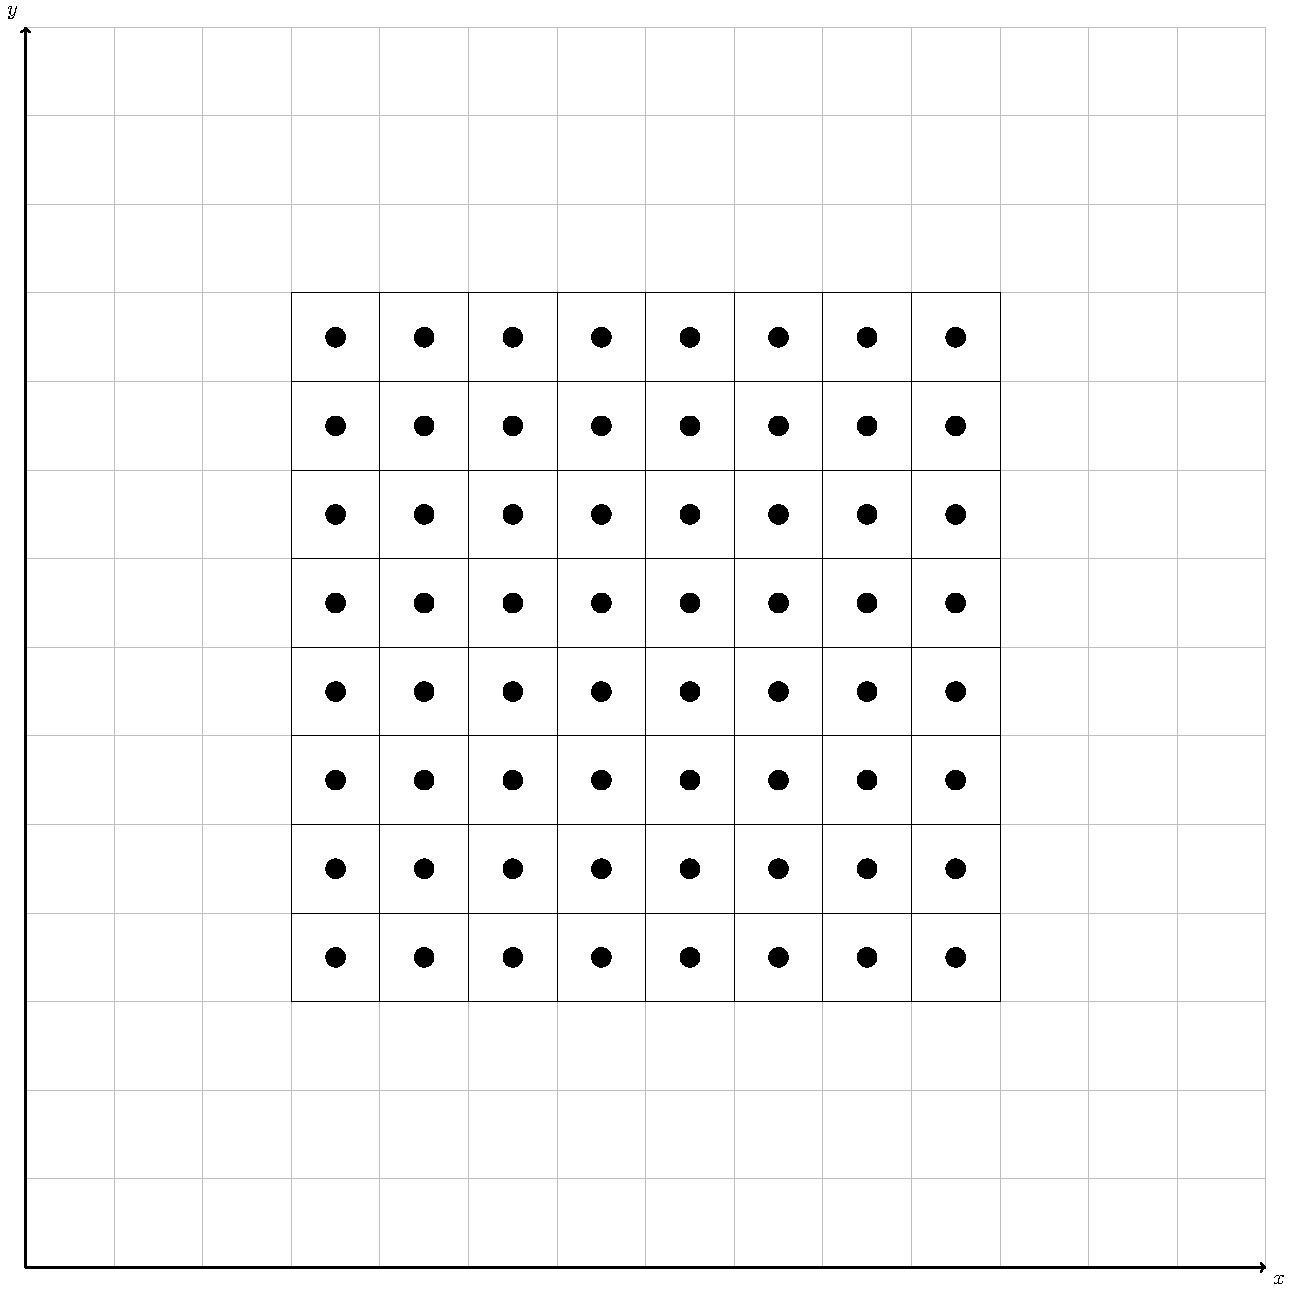
\includegraphics[width=1\linewidth]{2d_grid_GFQ}
		\caption{$Q^{yx,n}$ (black circles) after advecting $Q^{x,n}$ in $y$ direction. \label{lt-GFQx}}
    \end{subfigure}
	\caption{Illustration of the Lie-Trotter splitting applied in the $x$ direction (operator $\mathbf{F}$)
	and then in the $y$ direction (operator $\mathbf{G}$). Interior cells are depicted using black lines,
	 while ghost cells are depicted using gray lines. 
	 All the winds shown are the ones used in the DP1 departure point scheme.
	 If the DP2 scheme is used, an additional layer of wind ghost values should be added at each boundary in (a) and (b). \label{ltxdir}}
\end{figure}


\begin{figure}[!htb]
	\centering
	\begin{subfigure}{0.3\textwidth}
		\centering
		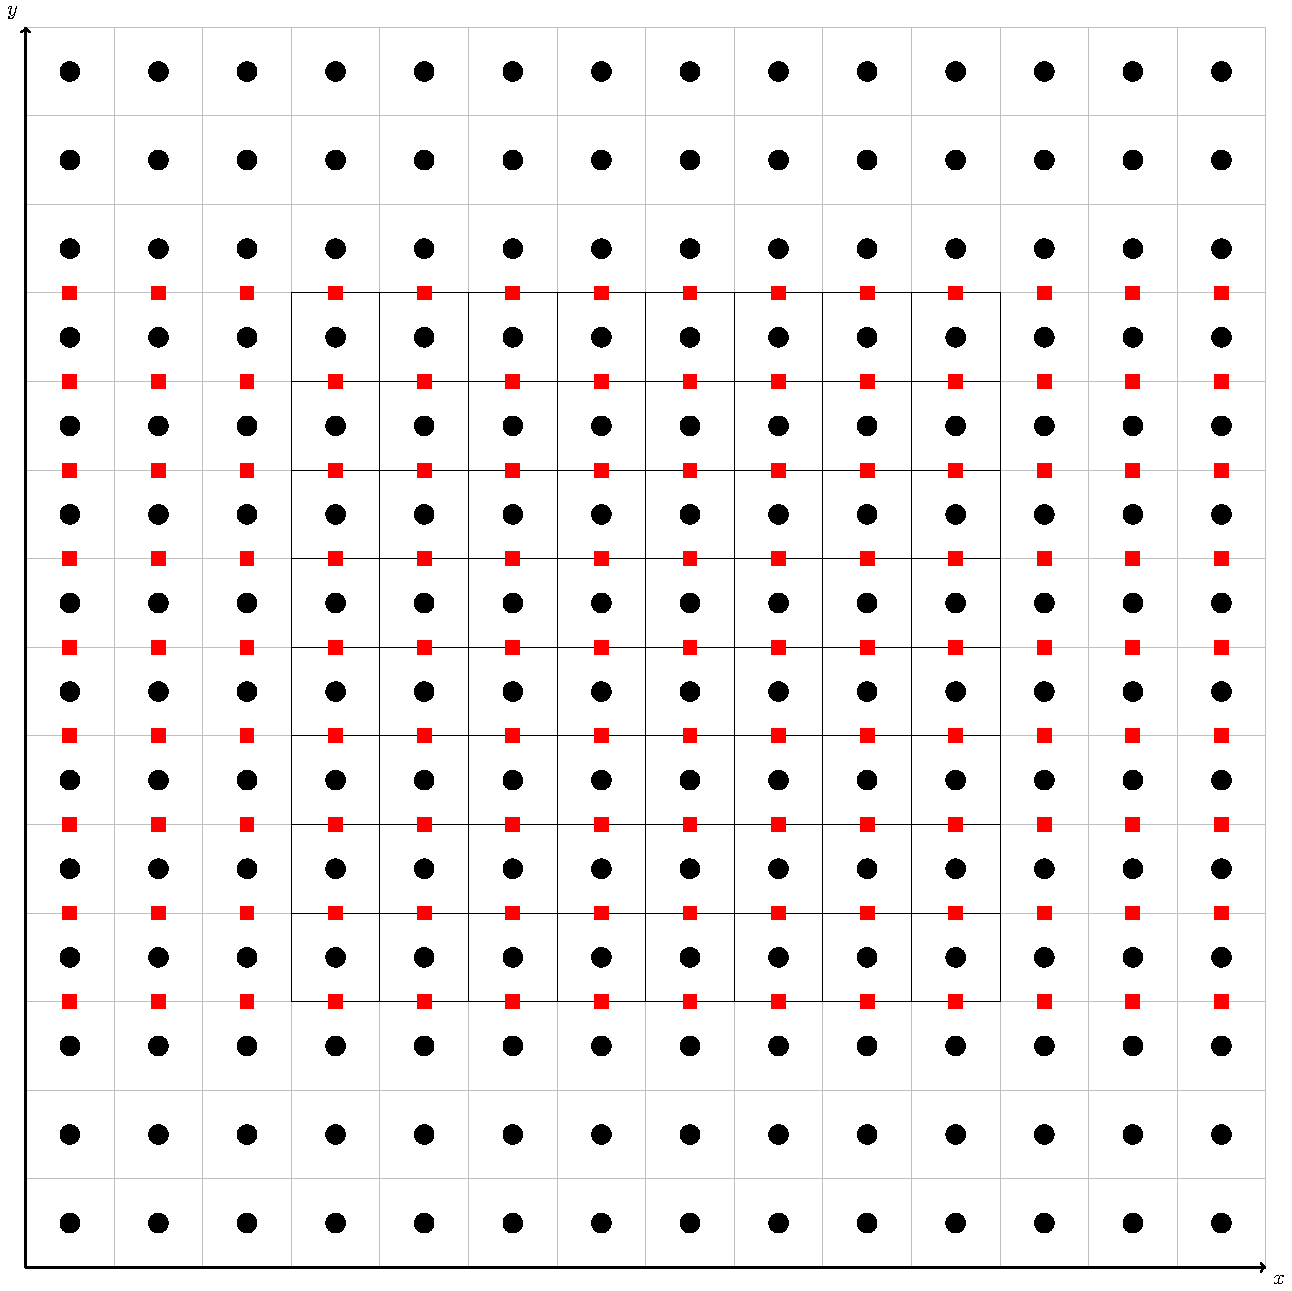
\includegraphics[width=1\linewidth]{2d_grid_Qy}
		\caption{$Q^n$ (black circles) and $v$ at edges (red squares). \label{lt-Qy}}
	\end{subfigure}
	\begin{subfigure}{0.3\textwidth}
		\centering
		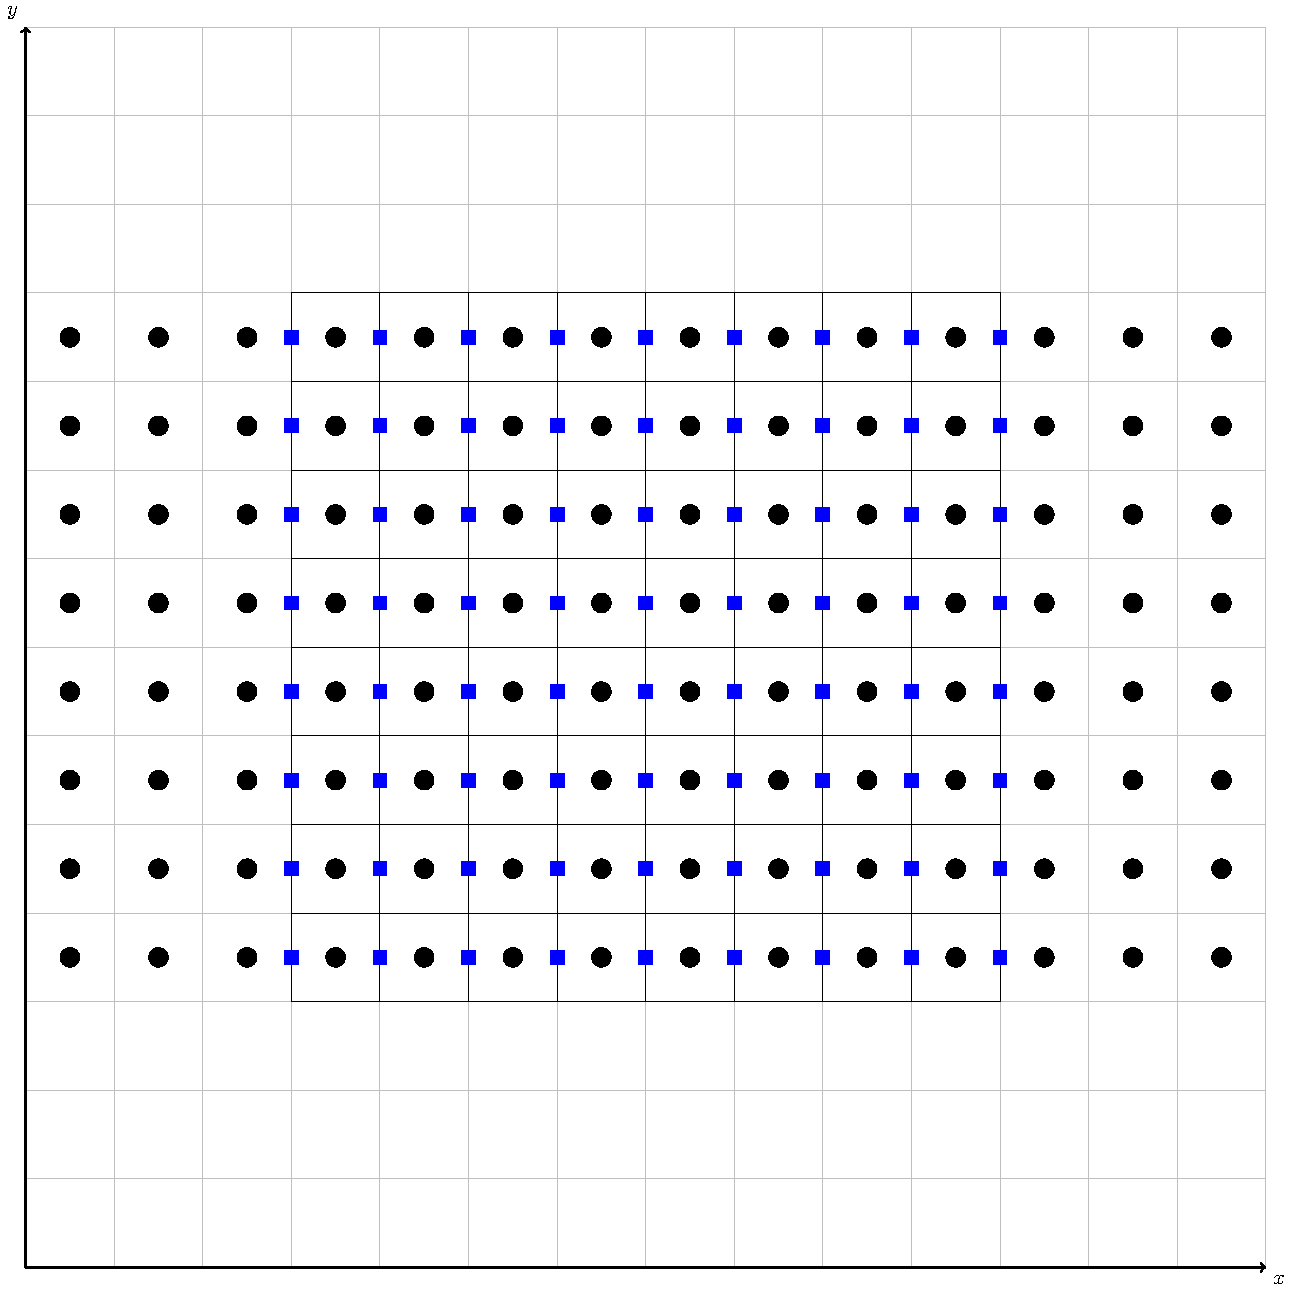
\includegraphics[width=1\linewidth]{2d_grid_GQ}
		\caption{$Q^{y,n}$ (black circles) and $u$ at edges (blue squares).\label{lt-GQy} }
	\end{subfigure}
	\begin{subfigure}{0.3\textwidth}
		\centering
		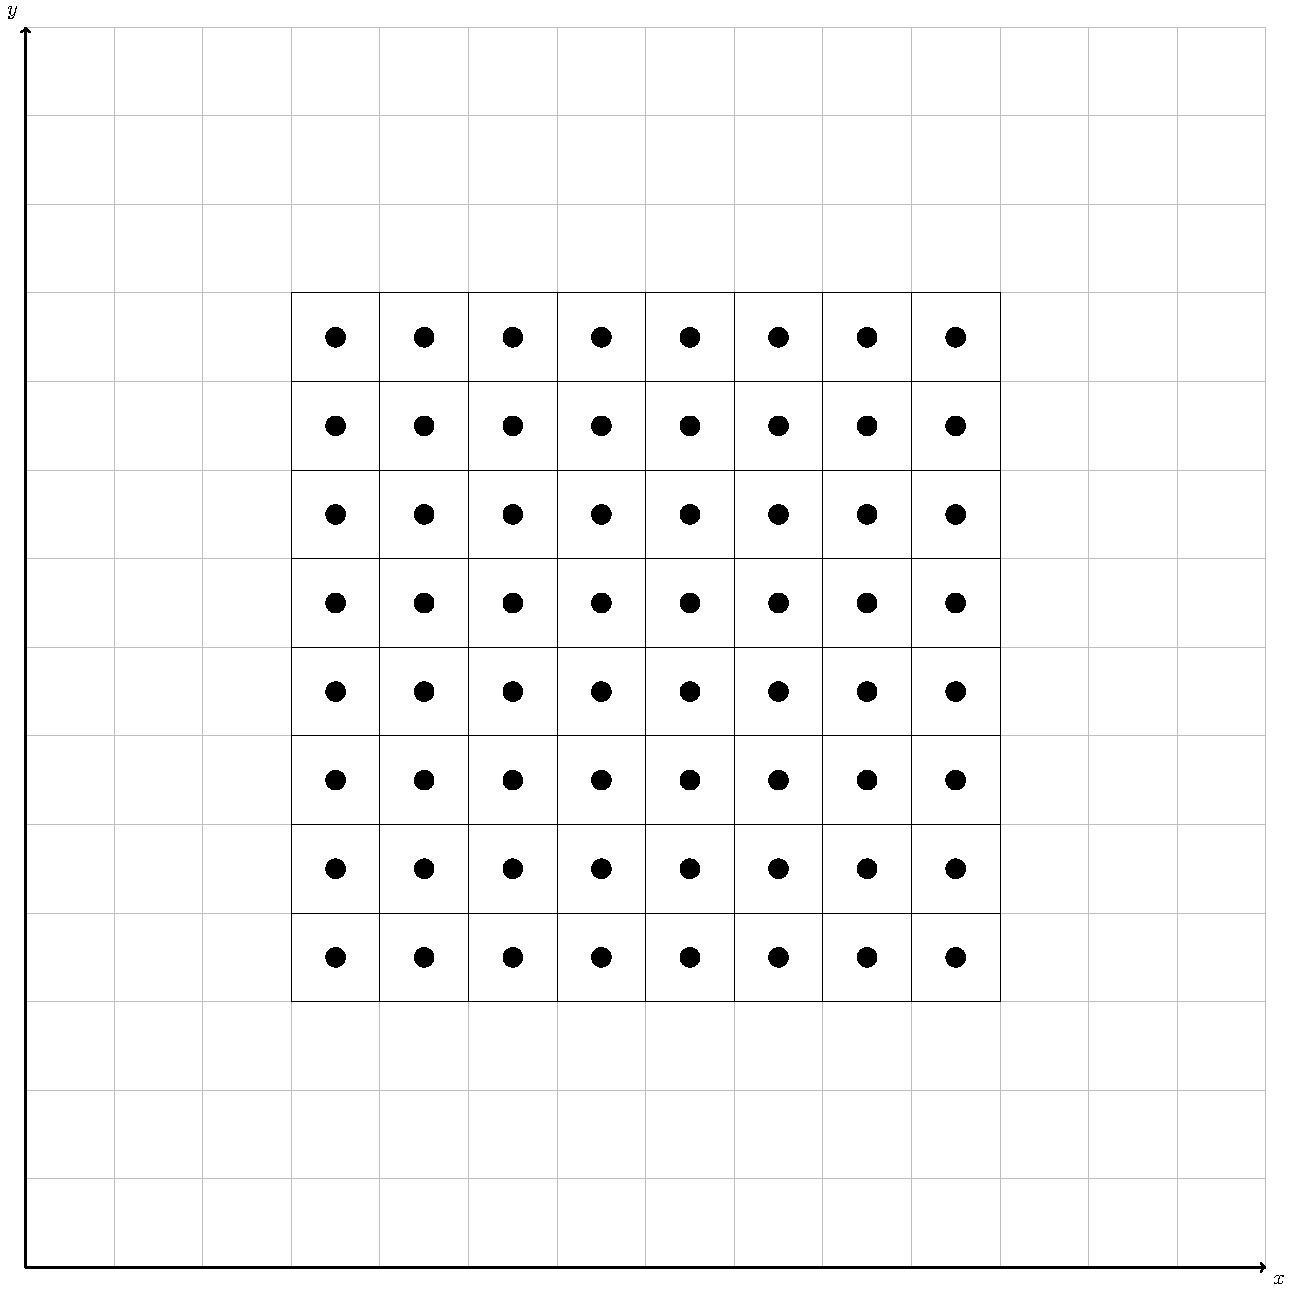
\includegraphics[width=1\linewidth]{2d_grid_GFQ}
		\caption{$Q^{xy,n}$ (black circles) after advecting $Q^{y,n}$ in $x$ direction. \label{lt-FGQy}}
	\end{subfigure}
	\caption{Similar to Figure \ref{ltxdir} but considering the Lie-Trotter splitting in reverse order.}
\end{figure}

The Lie-Trotter splitting is obtained by solving the advection in the $x$ direction
\begin{align*}
	{Q}^{x,n}_{ij} =  {Q}^{n}_{ij} + \mathbf{F}_{ij}[{Q^n}, \tilde{c}^{x,n}],
\end{align*}
for $j=\nu+1, \ldots, M+\nu$, $i=1, \ldots, N$ (Figure \ref{lt-FQx}), and then we advect in the $y$ direction with initial data ${Q}^{x,n}$ 
\begin{align*}
	{Q}^{yx,n}_{ij} = Q^{x,n}_{ij} + \mathbf{G}_{ij}[{Q}^{x,n},\tilde{c}^{y,n}],
\end{align*}
for $j=1, \ldots, M$,  $i=1, \ldots, N$  (Figure \ref{lt-GFQx}).
To get the average Lie-Trotter splitting we repeat the process in the reverse order by solving the advection equation
in the $y$ direction
\begin{align*}
	{Q}^{y,n}_{ij} =  {Q}^{n}_{ij} + \mathbf{G}_{ij}[{Q^n},\tilde{c}^{y,n}],
\end{align*}
for $i=-\nu+1, \ldots, N+\nu$, $j=1, \ldots, M$ (Figure \ref{lt-GQy}), and then we advect in the $x$-direction with initial data ${Q}^{y,n+1}$ 
\begin{align*}
	{Q}^{xy,n}_{ij} = Q^{y,n}_{ij} + \mathbf{F}_{ij}[Q^{y,n},\tilde{c}^{x,n}],
\end{align*}
for $i=1, \ldots, N$, $j=1, \ldots, M$ (Figure \ref{lt-FGQy}) and thus we have the average Lie-Trotter solution:
\begin{align}
\label{chp-adv2d-LT}
    Q^{n+1} = \frac{(Q^{xy,n} + Q^{yx,n})}{2} 
    = Q^n &+ \frac{1}{2}\mathbf{F}[Q^n,\tilde{c}^{x,n}] + \frac{1}{2}\mathbf{G}[Q^n,\tilde{c}^{y,n}] \nonumber \\
    &+\frac{1}{2}\mathbf{F}\bigg[Q^n + \mathbf{G}[Q^n, \tilde{c}^{y,n}], \tilde{c}^{x,n}\bigg]+
    \frac{1}{2}\mathbf{G}\bigg[Q^n + \mathbf{F}[Q^n, \tilde{c}^{x,n}], \tilde{c}^{y,n}\bigg].
\end{align}
This scheme shall be referred to in this work as the average Lie-Trotter (\textbf{LT}) scheme. 
Finally, we point out that this scheme could be built using any other 1D numerical flux function, 
but we focus on PPM since this is what is used in FV3.
\subsection{Elimination of splitting error for a constant scalar field and non-divergent wind}
\label{sp-error}
Let us, for an instant, assume that $\mathbf{F}$ and $\mathbf{G}$ are linear in their first input. This implies that Equation \eqref{chp-adv2d-LT} may be rewritten as:
\begin{align}
\label{chp-adv2d-LT-linear}
    Q^{n+1} = Q^n 
    &+ \mathbf{F}[Q^n,\tilde{c}^{x,n}] + \mathbf{G}[Q^n,\tilde{c}^{y,n}] \nonumber \\
    &+\frac{1}{2}\mathbf{F}\bigg[\mathbf{G}[Q^n, \tilde{c}^{y,n}], \tilde{c}^{x,n}\bigg]+
      \frac{1}{2}\mathbf{G}\bigg[\mathbf{F}[Q^n, \tilde{c}^{x,n}], \tilde{c}^{y,n}\bigg].
\end{align}
The numerical flux functions defined in Chapter \ref{chp-1d-fv} are indeed linear in the input $Q$ if there are no monotonic constraints,
that is, when we use the unlimited PPM (hord0),
implying that $\mathbf{F}$ and $\mathbf{G}$ are both linear in this case.
%citet{lin:1996} suggests using Equation \eqref{chp-adv2d-LT-linear}
%instead of \eqref{chp-adv2d-LT} to save computational operations, but the current implementation of FV3 does not follow this approach.
We are going to consider Equation \eqref{chp-adv2d-LT-linear}
even when there are monotonic constraints, to analyse the scheme when $\boldsymbol{u}$ is non-divergent ($\nabla \cdot 
\boldsymbol{u} = 0$) and the
scalar field is equal to a constant $\overline{q}$.
Then the solution remains constant. 
Since the wind is non-divergent, it follows from the Helmholtz decomposition theorem 
that there exists a stream function $\psi \in \mathcal{C}^2$ such that
\begin{align*}
    u(x,y,t) &= -\partial_y \psi(x,y,t),\\
    v(x,y,t) &= \partial_x \psi(x,y,t).
\end{align*}
Then, we may compute the wind using centered-finite differences 
\begin{align*}
    u_{i+\frac{1}{2},j}^{n}&=
    -\bigg(\frac{\psi_{i+\frac{1}{2},j+\frac{1}{2}}^{n}-\psi_{i+\frac{1}{2},j-\frac{1}{2}}^{n}}{\Delta y}\bigg),\\
    v_{i,j+\frac{1}{2}}^{n} &= 
    \frac{\psi_{i+\frac{1}{2},j+\frac{1}{2}}^{n}-\psi_{i-\frac{1}{2},j+\frac{1}{2}}^{n}}{\Delta x},\\
\end{align*}
and thus the following discrete divergence free condition holds
\begin{align}
\label{discrete-divfree}
  \frac{\delta_i u_{ij}^n}{\Delta x} + \frac{\delta_j v_{ij}^n}{\Delta y} = 0.
\end{align}
Notice that this identity holds for the time-averaged winds if we assume that
that $\tilde{u}^n$ and  $\tilde{v}^n$ are computed using DP1.
If we use DP2, this identity is no longer valid.
Now, using the fact that the scalar field is supposed to be constant, we have:
\begin{align*}
\mathbf{F}_{ij}[\overline{q},\tilde{c}^{x,n}] &= -\overline{q} \lambda \delta_i \tilde{u}_{ij}^n,\\
\mathbf{G}_{ij}[\overline{q},\tilde{c}^{y,n}] &= -\overline{q} \lambda \delta_j \tilde{v}_{ij}^n,
\end{align*}
recalling that $\lambda = \frac{\Delta t}{\Delta x} = \frac{\Delta t}{\Delta y}$.
Applying $\mathbf{G}$ and $\mathbf{F}$ again, we have:
\begin{align*}
\mathbf{G}_{ij}\big[\mathbf{F}[{\overline{q},\tilde{c}^{y,n}}],\tilde{c}^{x,n}\big] &= 
   \overline{q}\lambda^2 \bigg(
   \tilde{v}_{i,j+\frac{1}{2}}^n\mathfrak{F}_{i,j+\frac{1}{2}}^{PPM,y}[ {\delta_i} \tilde{u}_{ij}^n,\tilde{c}^{y,n}] 
-  \tilde{v}_{i,j-\frac{1}{2}}^n\mathfrak{F}_{i,j-\frac{1}{2}}^{PPM,y}[ {\delta_i} \tilde{u}_{ij}^n,\tilde{c}^{y,n}]\bigg)\\
&=  \overline{q}\lambda^2\delta_i \big( \tilde{v}_{ij}^n\mathfrak{F}_{ij}^{PPM,y}[ {\delta_i} \tilde{u}_{ij}^n,\tilde{c}^{y,n}] \big),
\end{align*}
\begin{align*}
\mathbf{F}_{ij}\big[\mathbf{G}[{\overline{q},\tilde{c}^{x,n}}],\tilde{c}^{y,n}\big] &= 
   \overline{q}\lambda^2 \bigg(
   \tilde{u}_{i,j+\frac{1}{2}}^n\mathfrak{F}_{i,j+\frac{1}{2}}^{PPM,x}[ {\delta_j} \tilde{v}_{ij}^n,\tilde{c}^{x,n}] 
-  \tilde{u}_{i,j-\frac{1}{2}}^n\mathfrak{F}_{i,j-\frac{1}{2}}^{PPM,x}[ {\delta_j} \tilde{v}_{ij}^n,\tilde{c}^{x,n}] \bigg)\\
&=  \overline{q}\lambda^2\delta_j \big( \tilde{u}_{ij}^n\mathfrak{F}_{ij}^{PPM,x}[ {\delta_j} \tilde{v}_{ij}^n,\tilde{c}^{x,n}] \big).
\end{align*}
However, if we compute the updated solution using Equation \eqref{chp-adv2d-LT-linear} we have that the error is given by
\begin{align}
	\label{chp-adv2d-LT-error}
	Q^{n+1}_{ij} - \overline{q} &= 
	-\Delta t \bigg(\frac{\delta_i \tilde{u}_{ij}^n}{\Delta x} + \frac{\delta_j \tilde{v}_{ij}^n}{\Delta y} \bigg)
	-\frac{\overline{q}}{2}\lambda^2
	\bigg(
	\delta_j \big( \tilde{u}_{ij}^n\mathfrak{F}_{ij}^{PPM,x}[ {\delta_j} \tilde{v}_{ij}^n,\tilde{c}^{x,n}] \big)+
        \delta_i \big( \tilde{v}_{ij}^n\mathfrak{F}_{ij}^{PPM,y}[ {\delta_i} \tilde{u}_{ij}^n,\tilde{c}^{y,n}] \big)\bigg) \nonumber\\
	&=
	-\frac{\overline{q}}{2}\lambda^2
	\bigg(
	\delta_j \big( \tilde{u}_{ij}^n\mathfrak{F}_{ij}^{PPM,x}[ {\delta_j} \tilde{v}_{ij}^n,\tilde{c}^{x,n}] \big)+
        \delta_i \big( \tilde{v}_{ij}^n\mathfrak{F}_{ij}^{PPM,y}[ {\delta_i} \tilde{u}_{ij}^n,\tilde{c}^{y,n}] \big)\bigg),
\end{align}
To eliminate this error, \citet{lin:1996} proposed modifying the Equation \eqref{chp-adv2d-LT} to
\begin{align}
\label{chp-adv2d-PL}
Q^{n+1} = Q^n &+ \frac{1}{2}\mathbf{F}[Q^n,\tilde{c}^{x,n}] + \frac{1}{2}\mathbf{G}[Q^n,\tilde{c}^{y,n}]\nonumber \\
&+\frac{1}{2}\mathbf{F}\bigg[Q^n + \mathbf{g}[Q^n, \tilde{c}^{y,n}], \tilde{c}^{x,n}\bigg]+
\frac{1}{2}\mathbf{G}\bigg[Q^n + \mathbf{f}[Q^n, \tilde{c}^{x,n}], \tilde{c}^{y,n}\bigg],
\end{align}
where $\mathbf{f}$ and $\mathbf{g}$ are called inner advective operators.
In this work, we shall consider the inner advective operator proposed by \citet{putman:2007} (hereafter referred to as \textbf{PL}).
The PL scheme is currently used in the FV3 dynamical core. Also, notice that the LT scheme is equivalent to the PL scheme but uses 
$\mathbf{f}=\mathbf{F}$ and $\mathbf{g}=\mathbf{G}$.
All the expressions for each inner advective operator mentioned are shown in Table \ref{chp-adv2d-tab1}.
\begin{table}[!h]
	\begin{tabular}{|c|l|l|}
		\hline
		Scheme & \multicolumn{1}{c|}{$\mathbf{f}_{ij}(Q^n, \tilde{c}^{x,n})$}
		       & \multicolumn{1}{c|}{$\mathbf{g}_{ij}(Q^n, \tilde{c}^{y,n})$} \\ \hline
		LT   & $\mathbf{F}_{ij}(Q^n,\tilde{c}^{x,n})$ 
		       & $\mathbf{G}_{ij}(Q^n,\tilde{c}^{y,n})$ \\ \hline
		PL   & $-Q_{ij}^n +
		         \frac{Q_{ij}^n  + \mathbf{F}_{ij}(Q^n,\tilde{c}^{x,n})}
			   {1 - \frac{1}{|\Omega_{ij}|}\big(\mathcal{A}_{i+\frac{1}{2},j}^{x} - \mathcal{A}_{i-\frac{1}{2},j}^{x}\big)}$
			   & $-Q_{ij}^n +
			 \frac{Q_{ij}^n  + \mathbf{G}_{ij}(Q^n,\tilde{c}^{y,n})}
			   {1 - \frac{1}{|\Omega_{ij}|}\ \big(\mathcal{A}_{i,j+\frac{1}{2}}^{y} - \mathcal{A}_{i,j-\frac{1}{2}}^{y}\big)}$
			   \\ \hline
	\end{tabular}
\caption{Expression of the inner advective operators considered in this work.
LT stands for the average Lie-Trotter  scheme, while PL stands for the scheme from \citet{putman:2007}.}
\label{chp-adv2d-tab1}
\end{table}
It is easy to see that the PL operator eliminates the term multiplied by $\lambda^2$ that appeared in Equation \eqref{chp-adv2d-LT-error}
when we apply these operators to a constant grid function $Q^n$ and a non-divergent velocity field in Equation \eqref{chp-adv2d-LT-error}.
Therefore, these inner advective operators eliminate the splitting error for a constant field and a non-divergent velocity field, making this scheme exact in this case
if we use DP1 to compute the departure points.
If we use DP2 with PL splitting, Equation \eqref{chp-adv2d-LT-error} will introduce a first-order error since the discrete divergence-free condition (Equation \eqref{discrete-divfree})
for the time-averaged winds of DP2 does not hold in this case.
We shall see this in the numerical experiments (Section \ref{sec-ds-exp}).
We point out that although the LT scheme has an error in Equation \eqref{chp-adv2d-LT-error}, it is a second-order error,
since this scheme is generally second-order accurate \citep{holden:2010}, provided that the 1D flux is second-order, 
which shall be the case if we use the DP2 scheme as discussed in Chapter \ref{chp-1d-fv}.

\section{Numerical experiments}
\label{sec-ds-exp}
To assess the dimension-splitting schemes LT and PL introduced previously, we are going to consider the linear advection 
equation on the spatial domain $[-\frac{L}{2},\frac{L}{2}]\times[-\frac{L}{2},\frac{L}{2}]$ and in the time interval $[0,T]$, 
with biperiodic boundary conditions, where $L = \frac{\pi}{2} R$. Here, $R = 6.371 \times 10^6$ meters, 
representing the Earth's radius, and $T = 1036800$ seconds, equivalent to 12 days. 
The spatial domain spans approximately $10^4$ kilometers in both directions,
which correspond to approximately the lengths of a cubed-sphere panel,
as shall be seen in Chapter \ref{chp-cs-grids}.

For the 1D schemes, we will consider the FV-SL unlimited PPM (\textbf{hord0} - Subsection \ref{chp-adv1d-sec-hord0}) and limited PPM
(\textbf{hord8}  - Subsection \ref{chp-adv1d-sec-hord8}), 
each tested with both departure point schemes \textbf{DP1} (Subsection \ref{chp-adv1d-sec-DP1}) and \textbf{DP2} (Subsection \ref{chp-adv1d-sec-DP2}).
We employ $(\Delta x^{(k)},\Delta y^{(k)},\lambda)$-discretizations with $\Delta x^{(k)} = \Delta y^{(k)} = \frac{L}{N^{(k)}}$,
$N^{(k)} = 48 \times 2^k$, $k=0,\ldots, 4$.
We introduce the relative error in the $p$-norm:
\begin{equation*}
	E_k = 
	\frac{\| Q^n - Q^0 \|_{p, \Delta x \times \Delta y}}
	{\|Q^0\|_{p, \Delta x \times \Delta y}}.
\end{equation*}
We are going to consider $p=1$ and $p=\infty$.
The convergence rate, as defined in Section \ref{chp-adv1d-sec-numerical-exp}, and the preservation of total mass variation with 
machine precision are considered in all experiments presented here.
It is worth noting that in error computation, we employ centroid values instead of exact average values to avoid 
the computation of analytical integrals.
This approximation, as discussed in Proposition \ref{prop-bound-centroid-2d}, introduces a second-order error.

\subsection{Square wave with constant wind advection}
For the initial test, a constant velocity $\boldsymbol{u}=\big(\frac{L}{T},\frac{L}{T}\big)$ is considered.
The IC is a rectangular profile (refer to Figure \ref{chp-adv2d-sec-exp-adv1-a}) given by:
\begin{equation}
	\label{chp-adv2d-ic1}
	q_0(x,y) =  
	\begin{cases}
		1 & \text{if } (x,y) \in [-0.1L,0.1L]\times [-0.1L,0.1L],\\
		0.1 & \text{otherwise}.
	\end{cases}
\end{equation}
\begin{figure}[!htb]
	\centering
	\begin{subfigure}{0.3\textwidth}
		\centering
		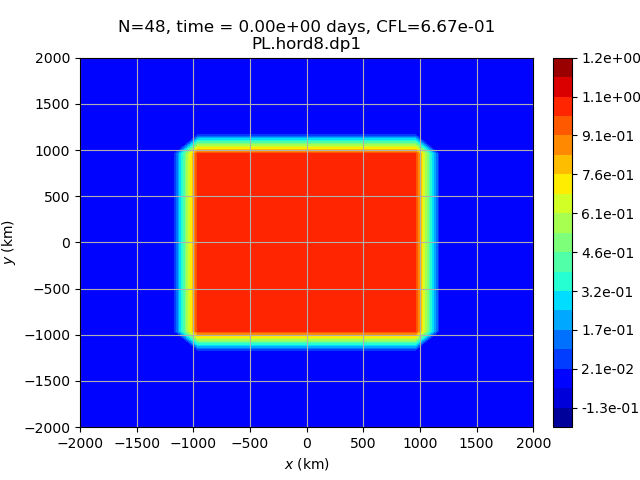
\includegraphics[width=1.185\linewidth]{adv2d_tc1_N48_hord8_iadv1_dp1_t0}
		\caption{IC\label{chp-adv2d-sec-exp-adv1-a}}
	\end{subfigure}
	\begin{subfigure}{0.3\textwidth}
		\centering
		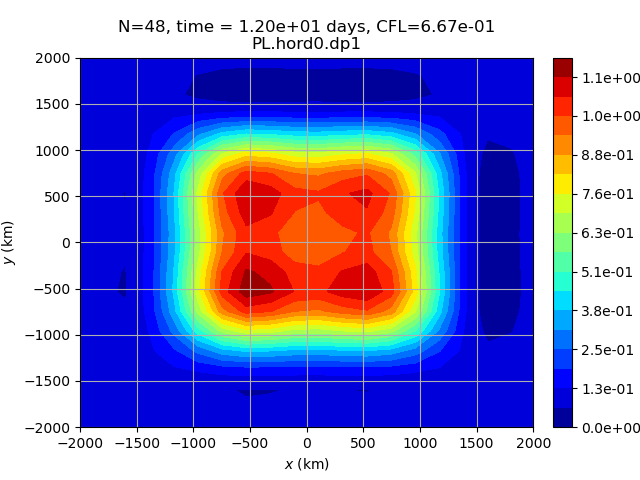
\includegraphics[width=1.185\linewidth]{adv2d_tc1_N48_hord0_iadv1_dp1_t12}
		\caption{PL-hord0\label{chp-adv2d-sec-exp-adv1-b}}
	\end{subfigure}
	\begin{subfigure}{0.3\textwidth}
		\centering
		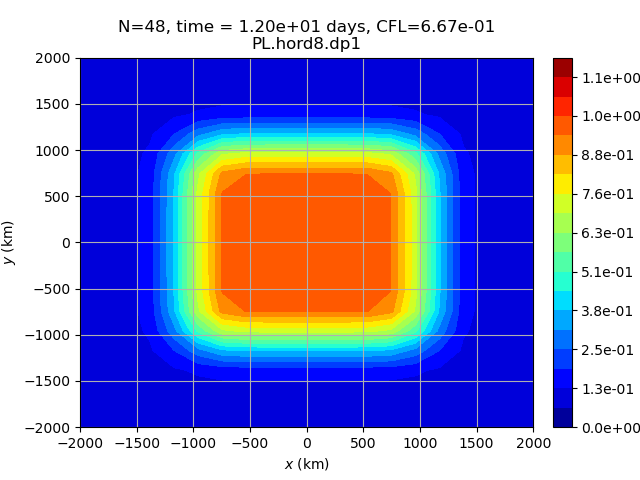
\includegraphics[width=1.185\linewidth]{adv2d_tc1_N48_hord8_iadv1_dp1_t12}
		\caption{PL-hord8.\label{chp-adv2d-sec-exp-adv1-c}}
	\end{subfigure}	
	\caption{Linear advection experiment using a constant velocity $\boldsymbol{u} = \left(\frac{L}{T},\frac{L}{T}\right)$, 
	a CFL number set to $0.67$, and a grid resolution of $N=M=48$.
	The initial condition is given by Equation \eqref{chp-adv2d-ic1}.
	We run this test with the PL splitting combined with the unlimited PPM (hord0) (b) and limited PPM (hord8) (c).
        The figures display the advected profile after 12 days (one time period).
        The initial condition is depicted in (a). \label{chp-adv2d-sec-exp-adv1}}
\end{figure}

We will employ a time step of 14400 seconds and set $N=M=48$ (therefore $\Delta x = \Delta y \approx 208$ km), resulting in a CFL number approximately equal to 0.67.
The exact solution of Problem \ref{chp-adv2d-sec2-prob1} in this scenario is $q_0((x,y)-\boldsymbol{u}t)$.
Due to the constant velocity field, all splitting schemes introduced in Section \ref{sec-dsplit} are equivalent.
Therefore, we only consider the PL splitting. Additionally, it is evident that the Lie-Trotter splitting is exact in this case 
(see, for example, \cite[p.~202-203]{leveque:1990}), meaning no splitting error is introduced.
For the 1D schemes, we utilize DP1 to compute the departure point, as this scheme is exact when the velocity is constant.

The conclusions drawn from this test closely resemble those of the first 1D test discussed in Section \ref{chp-adv1d-sec-numerical-exp-1}.
This similarity arises because no splitting error is introduced when the velocity remains constant.
Figure \ref{chp-adv2d-sec-exp-adv1-c} illustrates that PL splitting maintains monotonicity, particularly noticeable when using the limited 1D scheme hord8.

\newpage
\subsection{Flow deformation with nondivergent wind}
\label{2d-adv-ndivflow}
For a first variable velocity testing, we consider two Gaussian hills given by:
\begin{align}
	\begin{split}
	\label{chp-adv2d-ic2}
	q_0(x,y) = 0.1 + 0.9&\exp\bigg(-10\sin^2 \bigg(\pi \bigg(\frac{x}{L}-0.1\bigg)\bigg)\bigg) \exp\bigg(-10\sin^2 \bigg(\pi \frac{y}{L}\bigg) \bigg)+ \\
	           &\exp\bigg(-10\sin^2 \bigg(\pi \bigg(\frac{x}{L}+0.1\bigg)\bigg)\bigg) \exp\bigg(-10\sin^2 \bigg(\pi \frac{y}{L}\bigg) \bigg),
	\end{split}
\end{align}
defined in $[-\frac{L}{2},\frac{L}{2}] \times [-\frac{L}{2},\frac{L}{2}]$, whose graph is shown in Figure \ref{chp-adv2d-sec-exp-adv2-ic}.
\begin{figure}[!htb]
	\centering
	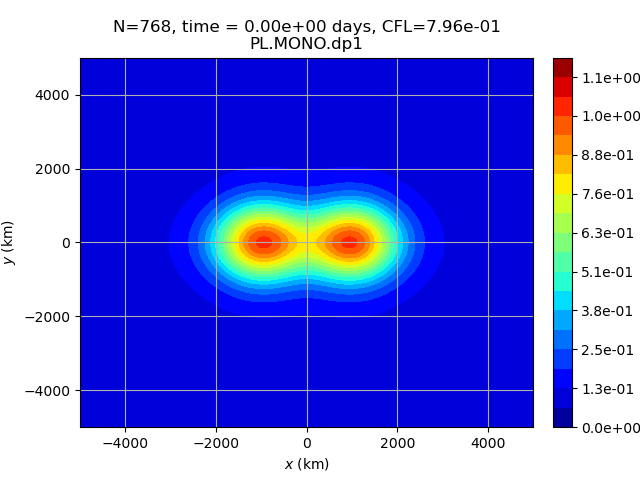
\includegraphics[width=0.5\linewidth]{adv2d_tc3_N768_hord8_iadv1_dp1_t0}
	\caption{Two Gaussian hills IC (Equation \eqref{chp-adv2d-ic2}). \label{chp-adv2d-sec-exp-adv2-ic}}
\end{figure}

We consider the Cartesian version of the deformational flow test case on the sphere from \citet{nair:2010}
proposed by \citet{chen:2017}. The velocity is given by:
\begin{equation}
	\label{chp-adv2d-vf1}
	\begin{cases}
		u(x,y,t) &= -c\frac{L}{T} \sin^2(\alpha_1)\sin\big(\frac{\pi y}{L}\big)\cos\big(\frac{\pi y}{L}\big)  \cos\big(\frac{\pi t}{T}\big) + \frac{L}{T},\\
		v(x,y,t) &= -2c\frac{L}{T}\sin(\alpha_1)  \cos(\alpha_1)\cos^2\big(\frac{\pi y}{L}\big)\cos\big(\frac{\pi t}{T}\big),
	\end{cases}
\end{equation}
where $\alpha_1 = 2\pi\big(\frac{x}{L}-\frac{t}{T}\big)$, $c = 10$.
\citet{chen:2017} uses periodic boundary conditions in the $x-$direction and zero-gradient in the $y-$direction.
However, we will employ biperiodic boundary conditions to simplify the problem.
This velocity field is divergence-free, and deforms the initial condition.
After $T$ time units (12 days in our case), the scalar field returns to its initial position and shape, allowing us to compute the error.
Notice that in Equation \eqref{chp-adv2d-vf1}, we have added a constant wind $\frac{L}{T}$ in the component
$u$ to prevent error cancellation, as discussed by \citet{nair:2010}.

Figure \ref{chp-adv2d-sec-exp-adv2} illustrates the results obtained using two Gaussian hills and the velocity field 
from Equation \eqref{chp-adv2d-vf1}.
We employed a high-resolution grid with $N=768$, along with the PL-DP1-hord8 scheme,
to demonstrate the behavior of the test.
The Figure shows the deformation of the scalar field over time, eventually returning to its initial position.

\begin{figure}[!htb]
	\centering
	\begin{subfigure}{0.3\textwidth}
		\centering
		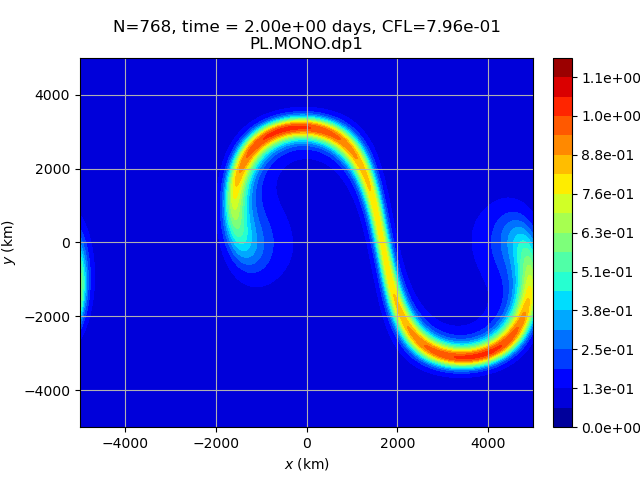
\includegraphics[width=1.2\linewidth]{adv2d_tc3_N768_hord8_iadv1_dp1_t2}
		\caption{$t=2$ days.\label{chp-adv2d-sec-exp-adv2-a}}
	\end{subfigure}
	\begin{subfigure}{0.3\textwidth}
		\centering
		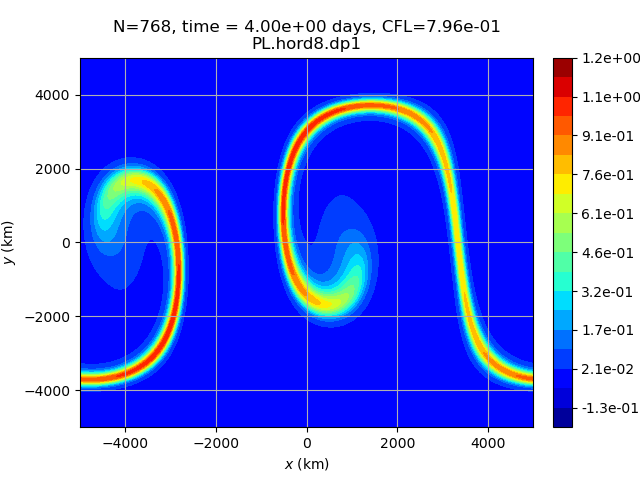
\includegraphics[width=1.2\linewidth]{adv2d_tc3_N768_hord8_iadv1_dp1_t4}
		\caption{$t=4$ days.\label{chp-adv2d-sec-exp-adv2-b}}
	\end{subfigure}

	\begin{subfigure}{0.3\textwidth}
		\centering
		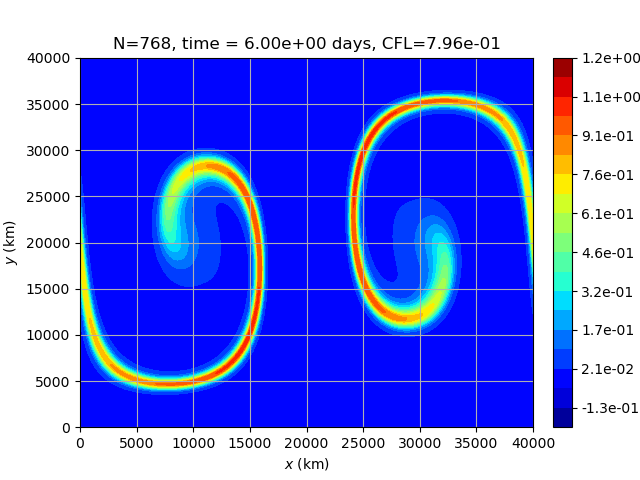
\includegraphics[width=1.2\linewidth]{adv2d_tc3_N768_hord8_iadv1_dp1_t6}
		\caption{$t=6$ days.\label{chp-adv2d-sec-exp-adv2-c}}
	\end{subfigure}
	\begin{subfigure}{0.3\textwidth}
		\centering
		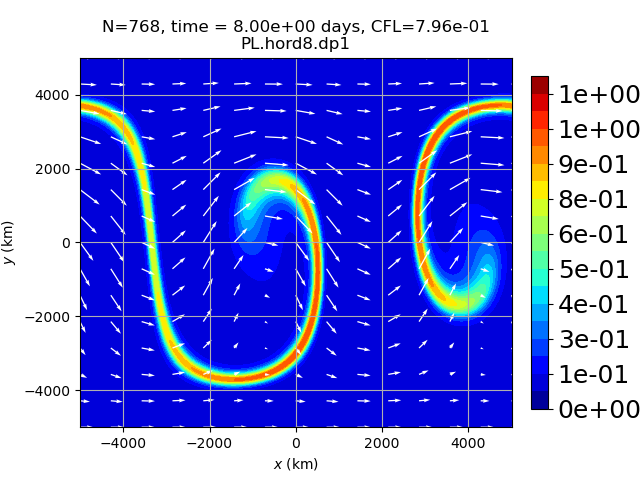
\includegraphics[width=1.2\linewidth]{adv2d_tc3_N768_hord8_iadv1_dp1_t8}
		\caption{$t=8$ days.\label{chp-adv2d-sec-exp-adv2-d}}
	\end{subfigure}

	\begin{subfigure}{0.3\textwidth}
		\centering
		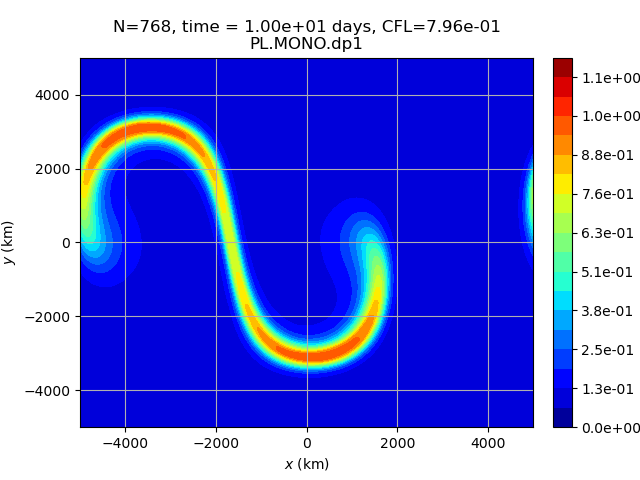
\includegraphics[width=1.2\linewidth]{adv2d_tc3_N768_hord8_iadv1_dp1_t10}
		\caption{$t=10$ days.\label{chp-adv2d-sec-exp-adv2-e}}
	\end{subfigure}
	\begin{subfigure}{0.3\textwidth}
		\centering
		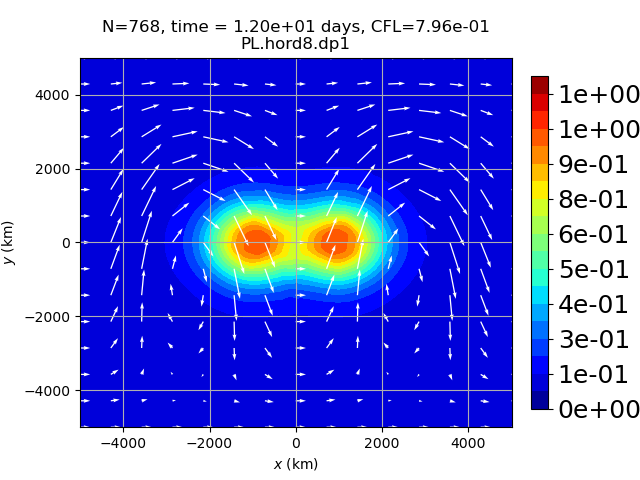
\includegraphics[width=1.2\linewidth]{adv2d_tc3_N768_hord8_iadv1_dp1_t12}
		\caption{$t=12$ days.\label{chp-adv2d-sec-exp-adv2-f}}
	\end{subfigure}
	\caption{Linear advection experiment using the velocity from Equation \eqref{chp-adv2d-vf1},
		a CFL number equal to $0.79$, $N=768$ cells, and the IC is given by 
		Equation \eqref{chp-adv2d-ic2}
		These figures show the advected profile at
		2 \eqref{chp-adv2d-sec-exp-adv2-a}, 
		4  \eqref{chp-adv2d-sec-exp-adv2-b},
		6  \eqref{chp-adv2d-sec-exp-adv2-c},
		8  \eqref{chp-adv2d-sec-exp-adv2-d},
		10  \eqref{chp-adv2d-sec-exp-adv2-e},
		and 12  \eqref{chp-adv2d-sec-exp-adv2-f} days.
		We are using the PL-DP1-hord8 scheme, where hord8 is the limited PPM. \label{chp-adv2d-sec-exp-adv2}}
\end{figure}

To investigate the error convergence, we employ time steps $\Delta t^{(k)}=\frac{5400}{2^{k}}$ for 
$k = 0, \ldots, 4$, and the spatial discretization as described at the beginning of Section \ref{sec-ds-exp},
resulting in a CFL number approximately equal to 0.79.

We can observe from Figure \ref{chp-adv2d-sec-exp-adv2-error-linf} that for the unlimited PPM (hord0), PL-DP1 and LT-DP2 have smaller
error and higher convergence order than PL-DP2 and LT-DP1.
However, when considering the limited PPM (hord8), all the schemes have the same error in $L_{\infty}$ norm.
The errors in $L_{1}$ norm (Figure \ref{chp-adv2d-sec-exp-adv2-error-l1}) exhibit a similar behavior; the only difference is 
that PL-DP1 and LT-DP2 have smaller errors than PL-DP2 and LT-DP1, along with higher convergence order.

\newpage

\begin{figure}[!htb]
\centering
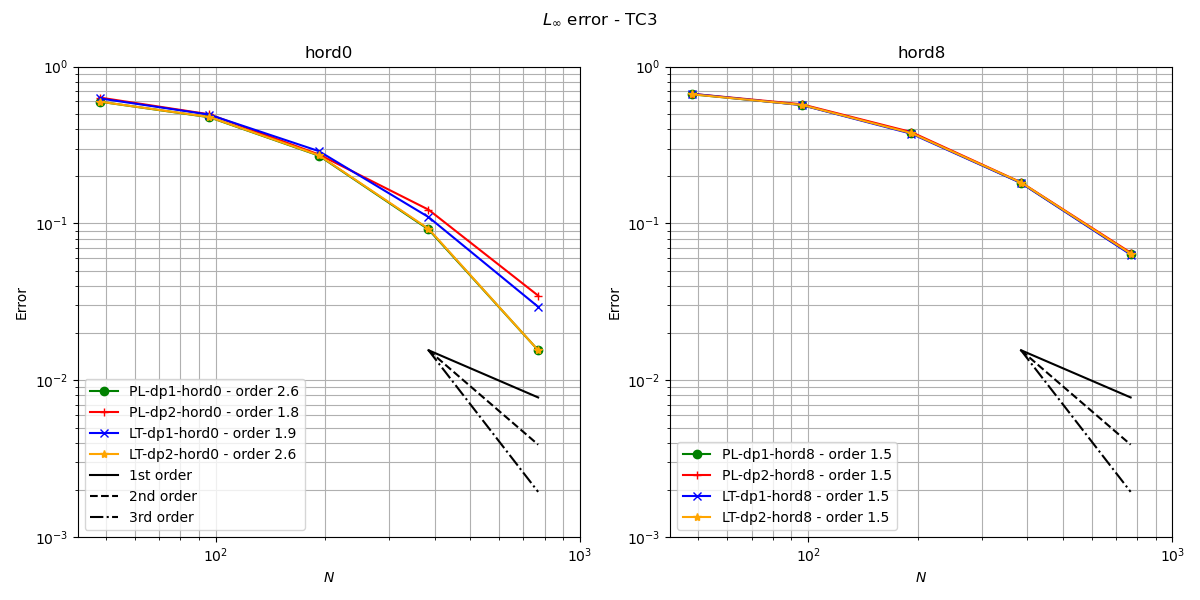
\includegraphics[width=1\linewidth]{adv2d_tc3_linf_error}
\caption{$L_{\infty}$ error for the two Gaussian hills (Equation \ref{chp-adv2d-ic2})
with the velocity from Equation \eqref{chp-adv2d-vf1}.
Schemes using the unlimited PPM (hord0) are on the left, and limited PPM (hord8) are on the right.
The PL scheme with DP1 is in green, and with DP2 is in red. 
The LT scheme with DP1 is in blue, and with DP2 is in yellow.
\label{chp-adv2d-sec-exp-adv2-error-linf}}
\end{figure}
\begin{figure}[!htb]
\centering
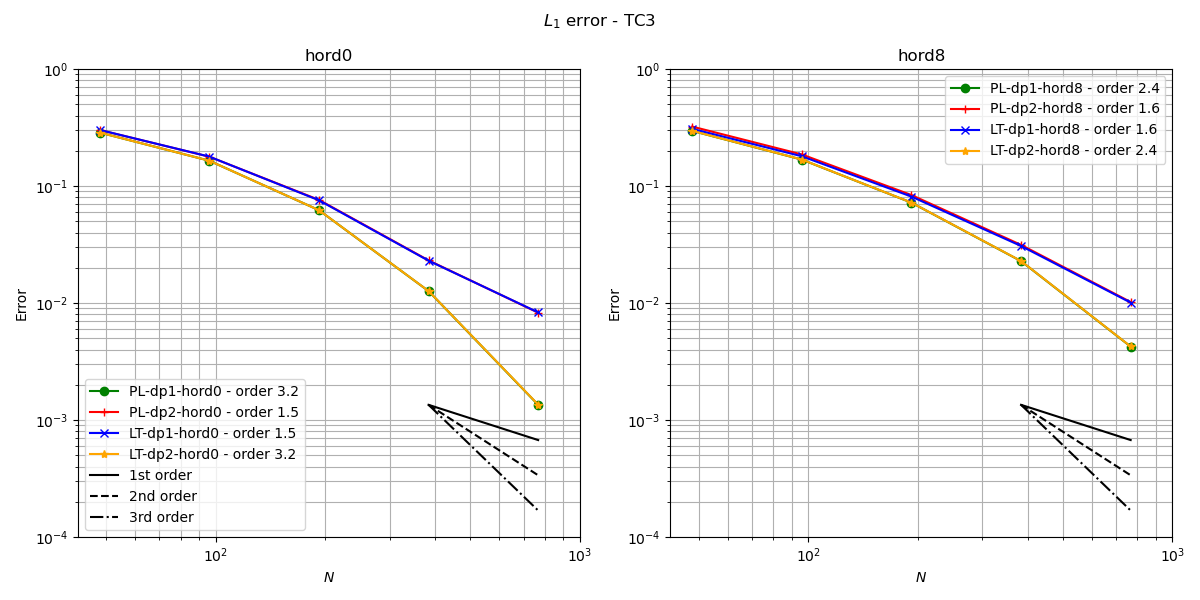
\includegraphics[width=1\linewidth]{adv2d_tc3_l1_error}
\caption{Similar to Figure \ref{chp-adv2d-sec-exp-adv2-error-linf} but considering the $L_1$ error.
\label{chp-adv2d-sec-exp-adv2-error-l1}}
\end{figure}

\newpage

\subsection{Flow deformation with divergent wind}
\label{2d-adv-divflow}
For a second variable velocity testing, we consider two Gaussian hills given by Equation 
\eqref{chp-adv2d-ic2} and the following wind:
\begin{equation}
	\label{chp-adv2d-vf2}
	\begin{cases}
		u(x,y,t) &= -\frac{L}{T} \cos^2\big(\frac{\pi x}{L}\big) \sin\big(\frac{2\pi y}{L}\big) \cos\big(\frac{\pi t}{T}\big), \\
		v(x,y,t) &= -\frac{L}{T} \cos^2\big(\frac{\pi y}{L}\big) \sin\big(\frac{2\pi x}{L}\big) \cos\big(\frac{\pi t}{T}\big).
	\end{cases}
\end{equation}
This test is based on the planar test from \citet{nair:2010}, but we adapt it to make the wind divergent.
Figure \ref{chp-adv2d-sec-exp-adv3} illustrates the results obtained using two Gaussian hills and the velocity field 
from Equation \eqref{chp-adv2d-vf2}, similarly to Figure  \ref{chp-adv2d-sec-exp-adv2}.
Again, the IC returns to its initial position after 12 days, allowing us to compute the error.

We employ time steps $\Delta t^{(k)}=\frac{14400}{2^{k}}$ for 
$k = 0, \ldots, 4$, to analyse the error convergence, 
along with the spatial discretization as described at the beginning of Section \ref{sec-ds-exp},
resulting in a CFL number approximately equal to 0.67.
\begin{figure}[!htb]
	\centering
	\begin{subfigure}{0.25\textwidth}
		\centering
		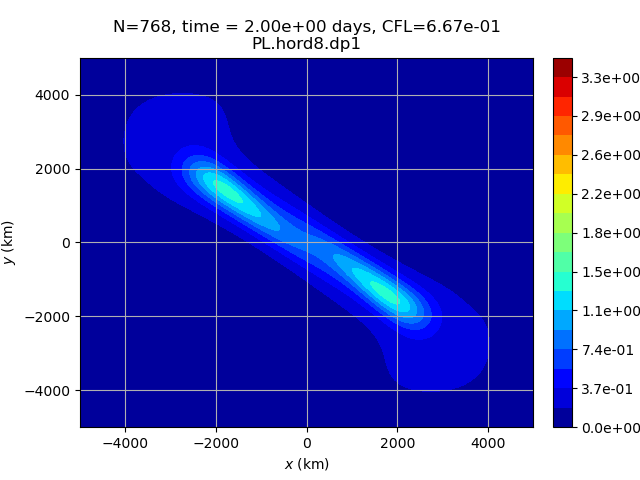
\includegraphics[width=1\linewidth]{adv2d_tc4_N768_hord8_iadv1_dp1_t2}
		\caption{$t=2$ days.\label{chp-adv2d-sec-exp-adv3-a}}
	\end{subfigure}
	\begin{subfigure}{0.25\textwidth}
		\centering
		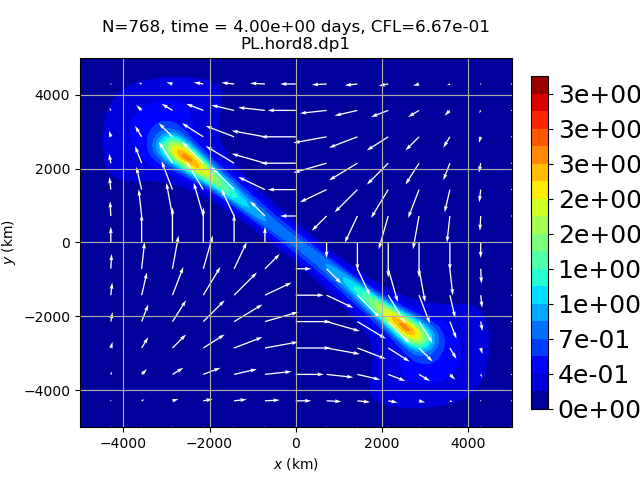
\includegraphics[width=1\linewidth]{adv2d_tc4_N768_hord8_iadv1_dp1_t4}
		\caption{$t=4$ days.\label{chp-adv2d-sec-exp-adv3-b}}
	\end{subfigure}
	\begin{subfigure}{0.25\textwidth}
		\centering
		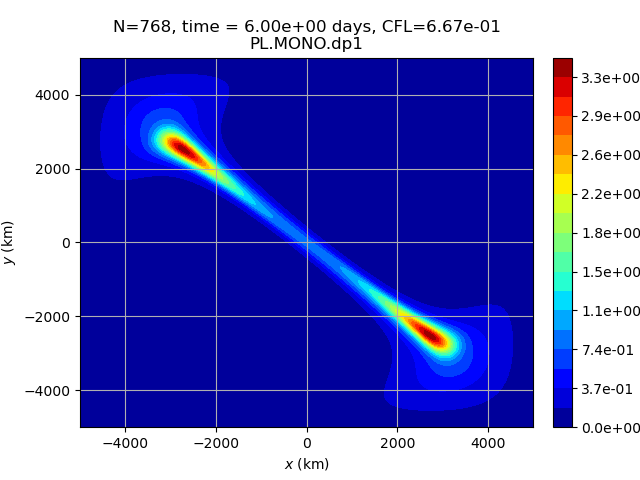
\includegraphics[width=1\linewidth]{adv2d_tc4_N768_hord8_iadv1_dp1_t6}
		\caption{$t=6$ days.\label{chp-adv2d-sec-exp-adv3-c}}
	\end{subfigure}
	
	\begin{subfigure}{0.25\textwidth}
		\centering
		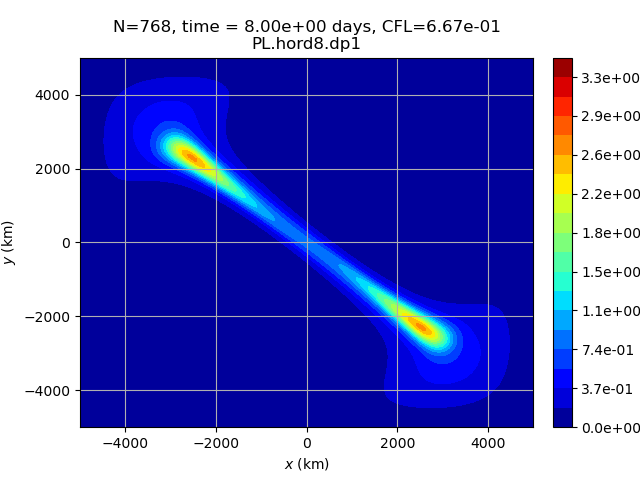
\includegraphics[width=1\linewidth]{adv2d_tc4_N768_hord8_iadv1_dp1_t8}
		\caption{$t=8$ days.\label{chp-adv2d-sec-exp-adv3-d}}
	\end{subfigure}
	\begin{subfigure}{0.25\textwidth}
		\centering
		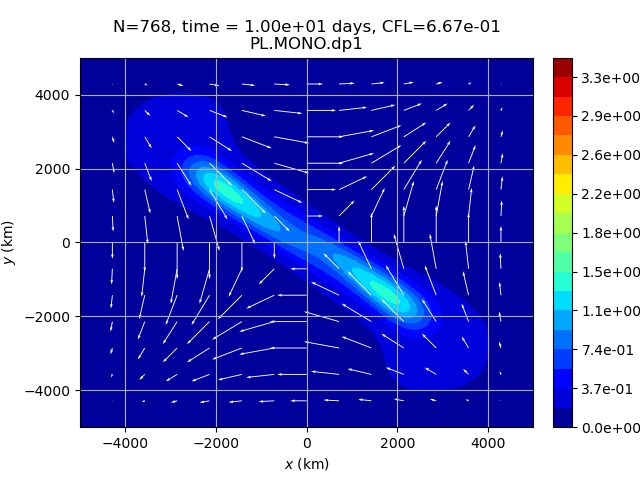
\includegraphics[width=1\linewidth]{adv2d_tc4_N768_hord8_iadv1_dp1_t10}
		\caption{$t=10$ days.\label{chp-adv2d-sec-exp-adv3-e}}
	\end{subfigure}
	\begin{subfigure}{0.25\textwidth}
		\centering
		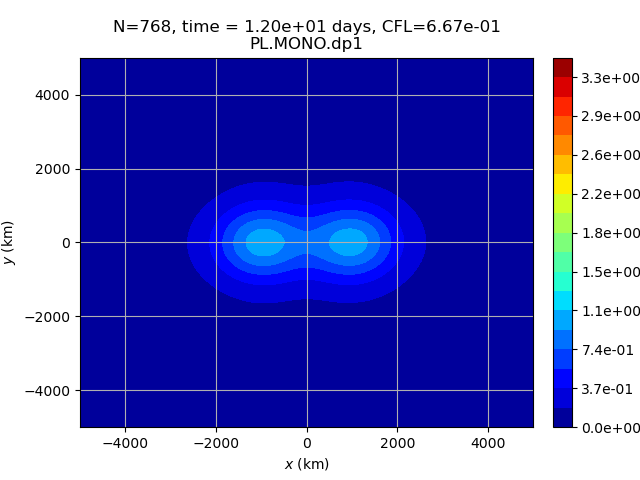
\includegraphics[width=1\linewidth]{adv2d_tc4_N768_hord8_iadv1_dp1_t12}
		\caption{$t=12$ days.\label{chp-adv2d-sec-exp-adv3-f}}
	\end{subfigure}
	\caption{Similar to Figure \ref{chp-adv2d-sec-exp-adv2}
		but using the wind from Equation \eqref{chp-adv2d-vf2}.
		We are using the PL-DP1-hord8 scheme, where hord8 is the limited PPM.\label{chp-adv2d-sec-exp-adv3}}
\end{figure}

We can observe from Figure \ref{chp-adv2d-sec-exp-adv3-error-linf} that for the unlimited PPM hord0, PL-DP1 has the bigger error,
while LT-DP2 has the smaller error and the highest convergence rate.
However, when considering the limited PPM (hord8) scheme, all the schemes have almost the same error in $L_{\infty}$ norm.
Regarding the error in $L_{1}$ norm (Figure \ref{chp-adv2d-sec-exp-adv3-error-l1}), we can see that for limited PPM (hord8),
LT-DP2 achieves second-order accuracy, while PL-DP1 achieves only first order.
Finally, the schemes PL-DP2 and LT-DP1 have the same errors for both the unlimited (hord0) and limited (hord8) PPM, in both $L_{\infty}$ and $L_{1}$ norms.

\newpage
\begin{figure}[!htb]
	\centering
	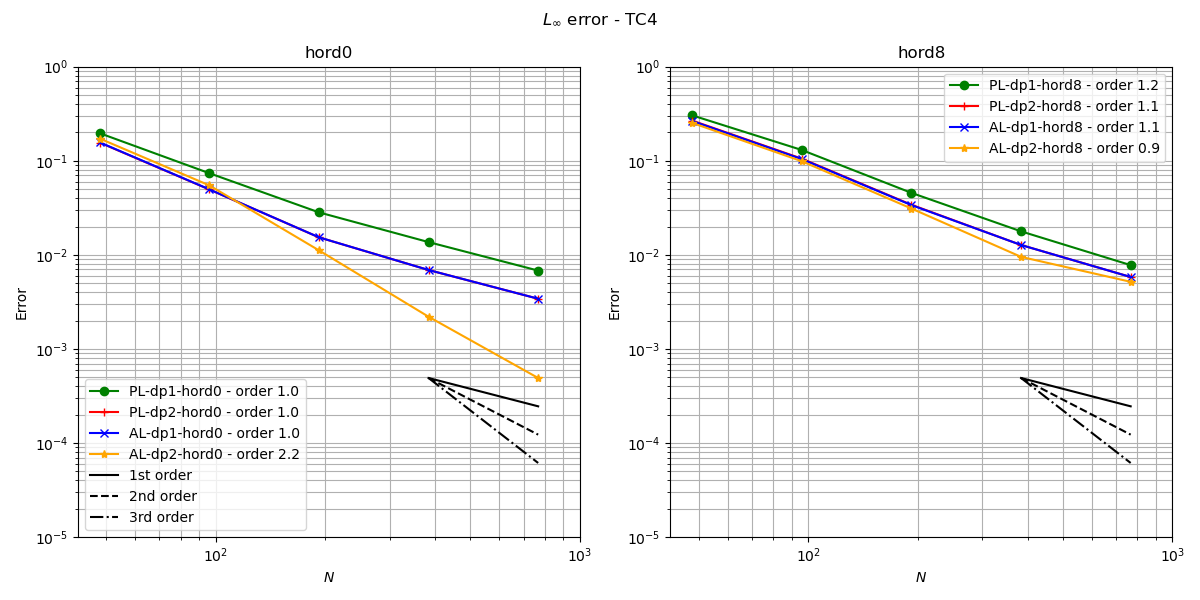
\includegraphics[width=1\linewidth]{adv2d_tc4_linf_error}
	\caption{$L_{\infty}$ error for the two Gaussian hills (Equation \ref{chp-adv2d-ic2})
			with the velocity from Equation \eqref{chp-adv2d-vf2}.
			Schemes using the unlimited PPM (hord0) are on the left, and limited PPM (hord8) are on the right.
			The PL scheme with DP1 is in green, and with DP2 is in red. 
			The LT scheme with DP1 is in blue, and with DP2 is in yellow.\label{chp-adv2d-sec-exp-adv3-error-linf}}
\end{figure}

\begin{figure}[!htb]
	\centering
	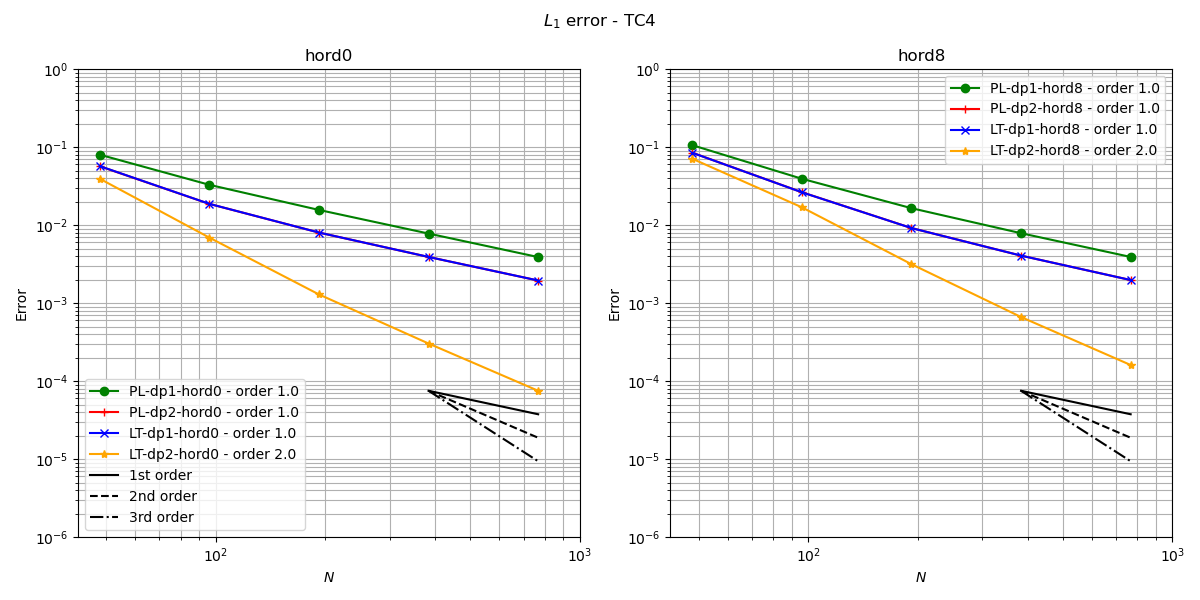
\includegraphics[width=1\linewidth]{adv2d_tc4_l1_error}
	\caption{Similar to Figure \ref{chp-adv2d-sec-exp-adv3-error-linf} but considering the $L_1$ error.
		\label{chp-adv2d-sec-exp-adv3-error-l1}}
\end{figure}

\newpage
\section{Concluding remarks}
\label{chp-2d-fv-conc}
In this Chapter, we introduced the dimension-splitting method, 
which replaces the solution of the 2D advection equation with the
solution of multiple 1D advection equations, resulting in more cost-effective 2D-FV schemes. 
For our simulations, we adopted the 1D FV-SL scheme based on PPM to solve the 1D equations.

We modified the average of two Lie-Trotter splittings, which is second-order accurate, 
to ensure the preservation of a constant scalar field with a divergence-free velocity,
following the works of \citet{lin:1996} and \citet{putman:2007}.
This modification addresses the limitation of the classical averaging Lie-Trotter splitting and follows the methodology used in FV3.

Based on the simulation with constant velocity, we concluded that all the splitting schemes
are equivalent and do not introduce any splitting errors. In fact, the splittings are exact in this case.
We observed that all the conclusions from the 1D simulations hold true in the 2D case as well,
with mass conservation and monotonicity being preserved when using the monotonic limiters in the 1D subproblems.

In the simulation with variable velocity, we conducted two flow deformation test cases.
For the divergence-free test, the schemes PL-DP1 and LT-DP2 showed similar behavior and performed better
than PL-DP2 and LT-DP1 in all error metrics analyzed here.
However, for the velocity with non-zero divergence, we observed that the scheme PL-DP1 achieved only
first-order accuracy and had larger errors than PL-DP2 and LT-DP1.
This limitation is because the PL-DP1 method is designed to be accurate for divergence-free winds.
This test highlights this limitation because we have divergence.
The scheme LT-DP2 showed better error performance, achieving second-order accuracy regardless of the non-divergence-free condition in the wind.
LT-DP2 also showed second-order accuracy in the $L_1$ norm when we employed the monotonic 1D flux, while PL-DP1 achieved first order.

In summary, the scheme PL-DP1, which is currently used in FV3 as the 2D advection solver, 
showed second-order accuracy for divergence-free winds, with LT-DP2 exhibiting similar behavior. 
However, for non-divergent free winds, LT-DP2 demonstrated second-order accuracy, while PL-DP1 achieved only first order.
\chapter{Cubed-sphere grids}
\label{chp-cs-grids}
So far, we have described the dimension-splitting technique in Chapter \ref{chp-2d-fv} for solving the advection equation on the plane.
Our current goal is to apply these schemes to solve the advection equation on the sphere.
Consequently, we need to introduce a grid over the sphere.
In order to facilitate the extension of dimension-splitting techniques onto the sphere, we require a logical Cartesian coordinate system, at least locally.

We point out that dimension-splitting schemes could be formulated in unstructured grids (see for instance \citet{herzfeld:2023}).
A good reason to use a locally Cartesian grid is to avoid problems, such as the lack of convergence of the divergence operator, among others,
that may arise in some grid cells within those grids \citep{peixoto:2013, peixoto:2016, weller:2012}.
Also, a logical Cartesian coordinate system eases the process of higher-order interpolation,
which can be more complicated on a spherical unstructured grid, requiring tangent plane approximations \citep{peixoto:2014,skamarock:2011}.

The scheme proposed by \citet{lin:1996} was originally implemented on latitude-longitude grids,
and the FV dynamical core was elucidated in \citet{lin:2004}.
The latitude-longitude grids exhibit convergence of meridians at the poles, 
necessitating the utilization of the Semi-Lagrangian formulation of PPM for larger CFL numbers,
as discussed in Section \ref{chp-adv1d-sec-flux}, 
to overcome the CFL restriction imposed by the poles.
However, this approach needs the processes in a parallel domain decomposition of the latitude-longitude grid to utilize more
data at the poles, resulting in less parallel efficiency.
Therefore, \citet{putman:2007} proposed considering the cubed-sphere (CS, hereafter) instead.
The CS grid is more uniform, thus not exhibiting a strong CFL condition anywhere.
This eliminates the need for the Semi-Lagrangian formulation of PPM, which is better for parallel efficiency, and led to the development of the FV3 core.

The CS grid was originally proposed by \citet{sadourny:1972} and was 
reinvestigated by \citet{ronchi:1996} and \citet{rancic:1996}. 
As is usual for Planotic grids, we start with a Platonic solid, in this case, a cube, 
which is circumscribed in a sphere. We then project its faces onto the sphere.
The original CS, called the equidistant CS, was proposed by 
\citet{sadourny:1972} but resulted in a non-uniform grid. 
To address this issue, a solution was proposed by introducing angular coordinates, 
leading to a quasi-uniform grid known as the equiangular CS.
The cubed sphere consists of six panels, each one having a local Cartesian coordinate 
system. 
As we pointed out before, this makes it easier to extend methods from the plane to the sphere. 
In fact, \citet{putman:2007} extends the dimension splitting technique from 
\citet{lin:1996}, as presented in Chapter \ref{chp-2d-fv}, to the CS.

There are essentially two major challenges when working with the CS grid:
\begin{enumerate}
\item
The non-orthogonal grid system: This challenge is primarily related to the appearance of
metric terms in the equations. It adds computational cost and often requires conversions
between contravariant and covariant components of a velocity field.
\item
The discontinuity of the coordinate system at the cube edges: This is perhaps the most 
problematic challenge. Computing stencils along the cube edges becomes challenging due to 
the discontinuous nature of the coordinate system.
\end{enumerate}
One possible approach to compute stencils at the edges is to extend the local coordinate 
of each panel to its neighboring panels, adding ghost cells in the halo region. In the 
case of the equiangular CS, ghost cell values lie on the same geodesics 
containing the data from the neighboring panels. This allows for the use of one-dimensional
high-order Lagrange interpolation to compute the stencils at the edges. 
This approach has been extensively used in the literature \citep{croisille:2013, 
katta:2015, katta:2015b, chen:2021} and was initially introduced by \citet{ronchi:1996}.
This approach is referred to as \textbf{duo-grid}, as named by \citet{chen:2021}.
Alternatively, \citet{putman:2007} uses extrapolation for the PPM reconstruction values near the cube edges.
Another approach that avoids the need for interpolation or extrapolation near the edges is 
the conformal CS developed by \citet{rancic:1996}. While this grid leads to an 
orthogonal and continuous coordinate system near the edges, it generates grid singularities
near the cube corners, similar to the pole problem. 
An improved and more uniform conformal grid, called the Uniform Jacobian cubed sphere, was 
later proposed by \citet{rancic:2017}.
Each approach is likely to generate grid imprinting, and one of the goals of this work is 
to investigate the amount of grid imprinting produced by different methods.

This Chapter aims to review and investigate the geometrical properties of the CS.
We start with a basic review of the CS mappings in Section \ref{cs-mappings}.
In Section \ref{sec-cs-grids}, we introduce the CS grids and investigate its geometrical properties.
Section \ref{cs-halodata} investigates how we can apply 1D Lagrange interpolation using the adjacent panels
data to obtain values of a scalar/vector field on ghost cells.
In Section \ref{cs-recon}, we compare the current extrapolation used in FV3 with Lagrange when using the PPM reconstruction to
remap the values from centers to edges on the cubed-sphere cells.
Final thoughts are presented in Section \ref{cs-conc}.

\newpage
\section{Cubed-sphere mappings}
\label{cs-mappings}
\subsection{Mapping between the cube and sphere}
\label{equidistant-cs}
We start this section by introducing the mapping between the cube and the sphere, which will divide the sphere into 6 quadrilaterals, also called panels, and allow us to tessellate the sphere into smaller quadrilaterals for panels.
Given $R>0$, we denote the sphere of radius $R$ 
centered at the origin of  $\mathbb{R}^3$ as:
\begin{equation*}
	\mathbb{S}^2_R = \{ P = (X,Y,Z) \in \mathbb{R}^3: X^2 + Y^2 + Z^2 = R^2\}.
\end{equation*}
We consider %$a = \frac{R}{\sqrt{3}}$ representing the half-length of the cube,and
the family of maps
$\boldsymbol{\Gamma}_{p}: [-1,1] \times [-1,1] \to \mathbb{S}^2_R$, $p=1, \ldots, 6$,
where:
\begin{equation*}
	\boldsymbol{\Gamma}_{1}(x,y) = \frac{R}{\sqrt{1 + x^2 + y^2}}(1, x, y), 
\end{equation*}
\begin{equation*}
	\boldsymbol{\Gamma}_{2}(x,y) = \frac{R}{\sqrt{1 + x^2 + y^2}}(-x, 1, y), 
\end{equation*}
\begin{equation*}
	\boldsymbol{\Gamma}_{3}(x,y) = \frac{R}{\sqrt{1 + x^2 + y^2}}(-1, -x, y), 
\end{equation*}
\begin{equation*}
	\boldsymbol{\Gamma}_{4}(x,y) = \frac{R}{\sqrt{1 + x^2 + y^2}}(x, -1, y), 
\end{equation*}
\begin{equation*}
	\boldsymbol{\Gamma}_{5}(x,y) = \frac{R}{\sqrt{1 + x^2 + y^2}}(-y, x, 1), 
\end{equation*}
\begin{equation*}
	\boldsymbol{\Gamma}_{6}(x,y) = \frac{R}{\sqrt{1 + x^2 + y^2}}(y, x, -1).
\end{equation*}


\begin{figure}[!htb]
	\centering
	\begin{subfigure}{0.42\textwidth}
		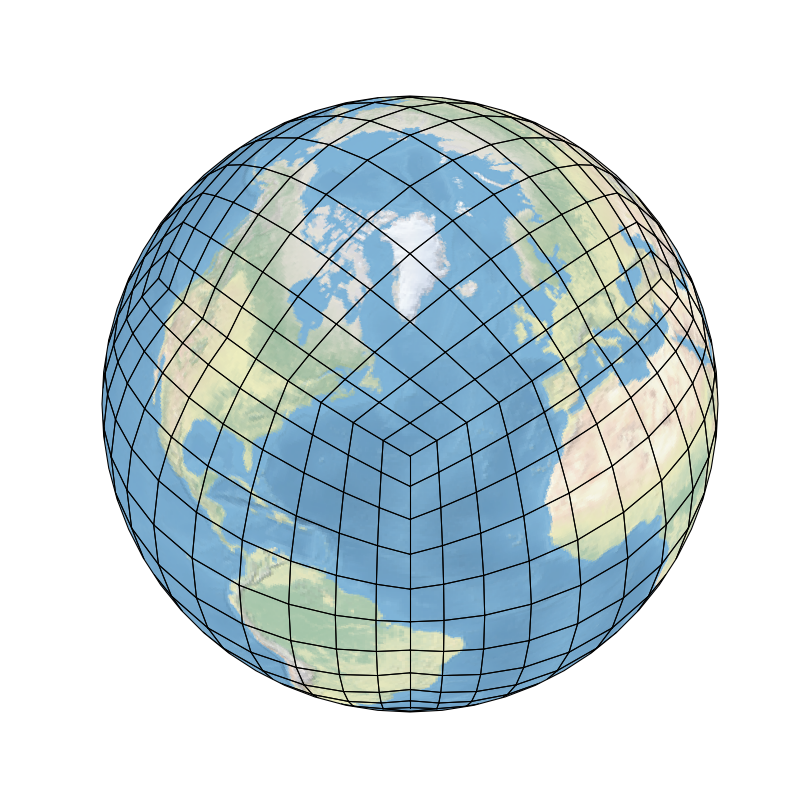
\includegraphics[width=1\linewidth]{gnomonic_equidistant_cs_10_sphere}
		\caption{Gridlines of the cube to the sphere mapping}
	\end{subfigure}
	\begin{subfigure}{0.42\textwidth}
		\centering
		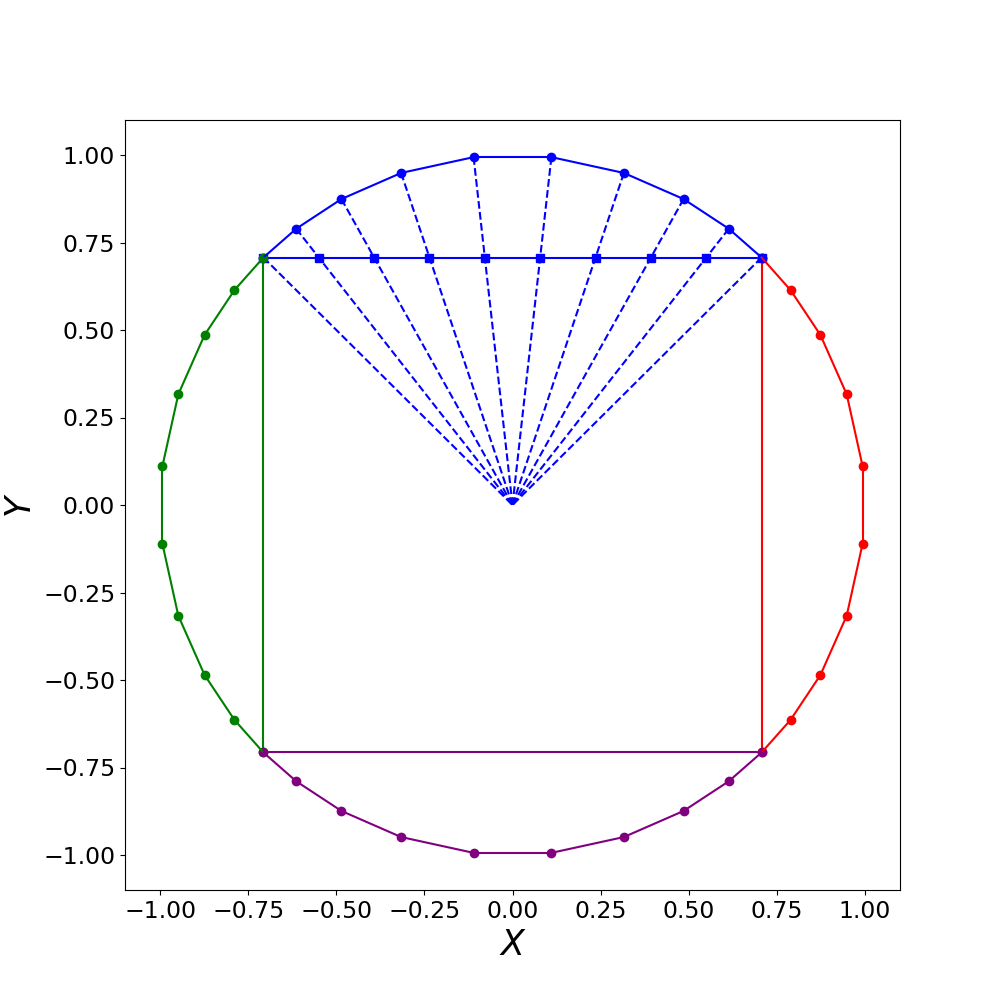
\includegraphics[width=1\linewidth]{g1}
		\caption{Cube and sphere mapping for $Z=0$.}
	\end{subfigure}
	\caption{(a) Illustration of the resulting cube-to-sphere mapping and (b) illustration of the cube-to-sphere projection.\label{chp-cs-equidistant}}
\end{figure}
The set of 6 maps $\{\boldsymbol{\Gamma}_{p}, p = 1, \ldots, 6\}$ allow us to cover the sphere (Figure \ref{chp-cs-equidistant}).
Here $p$ denotes a panel, and they are defined and orientated as Figure \ref{chp-cs-panels}
shows. Then, we can represent a point on the sphere using the cubed-sphere coordinates
$(x,y,p)$.

\begin{figure}[!htb]
	\centering
	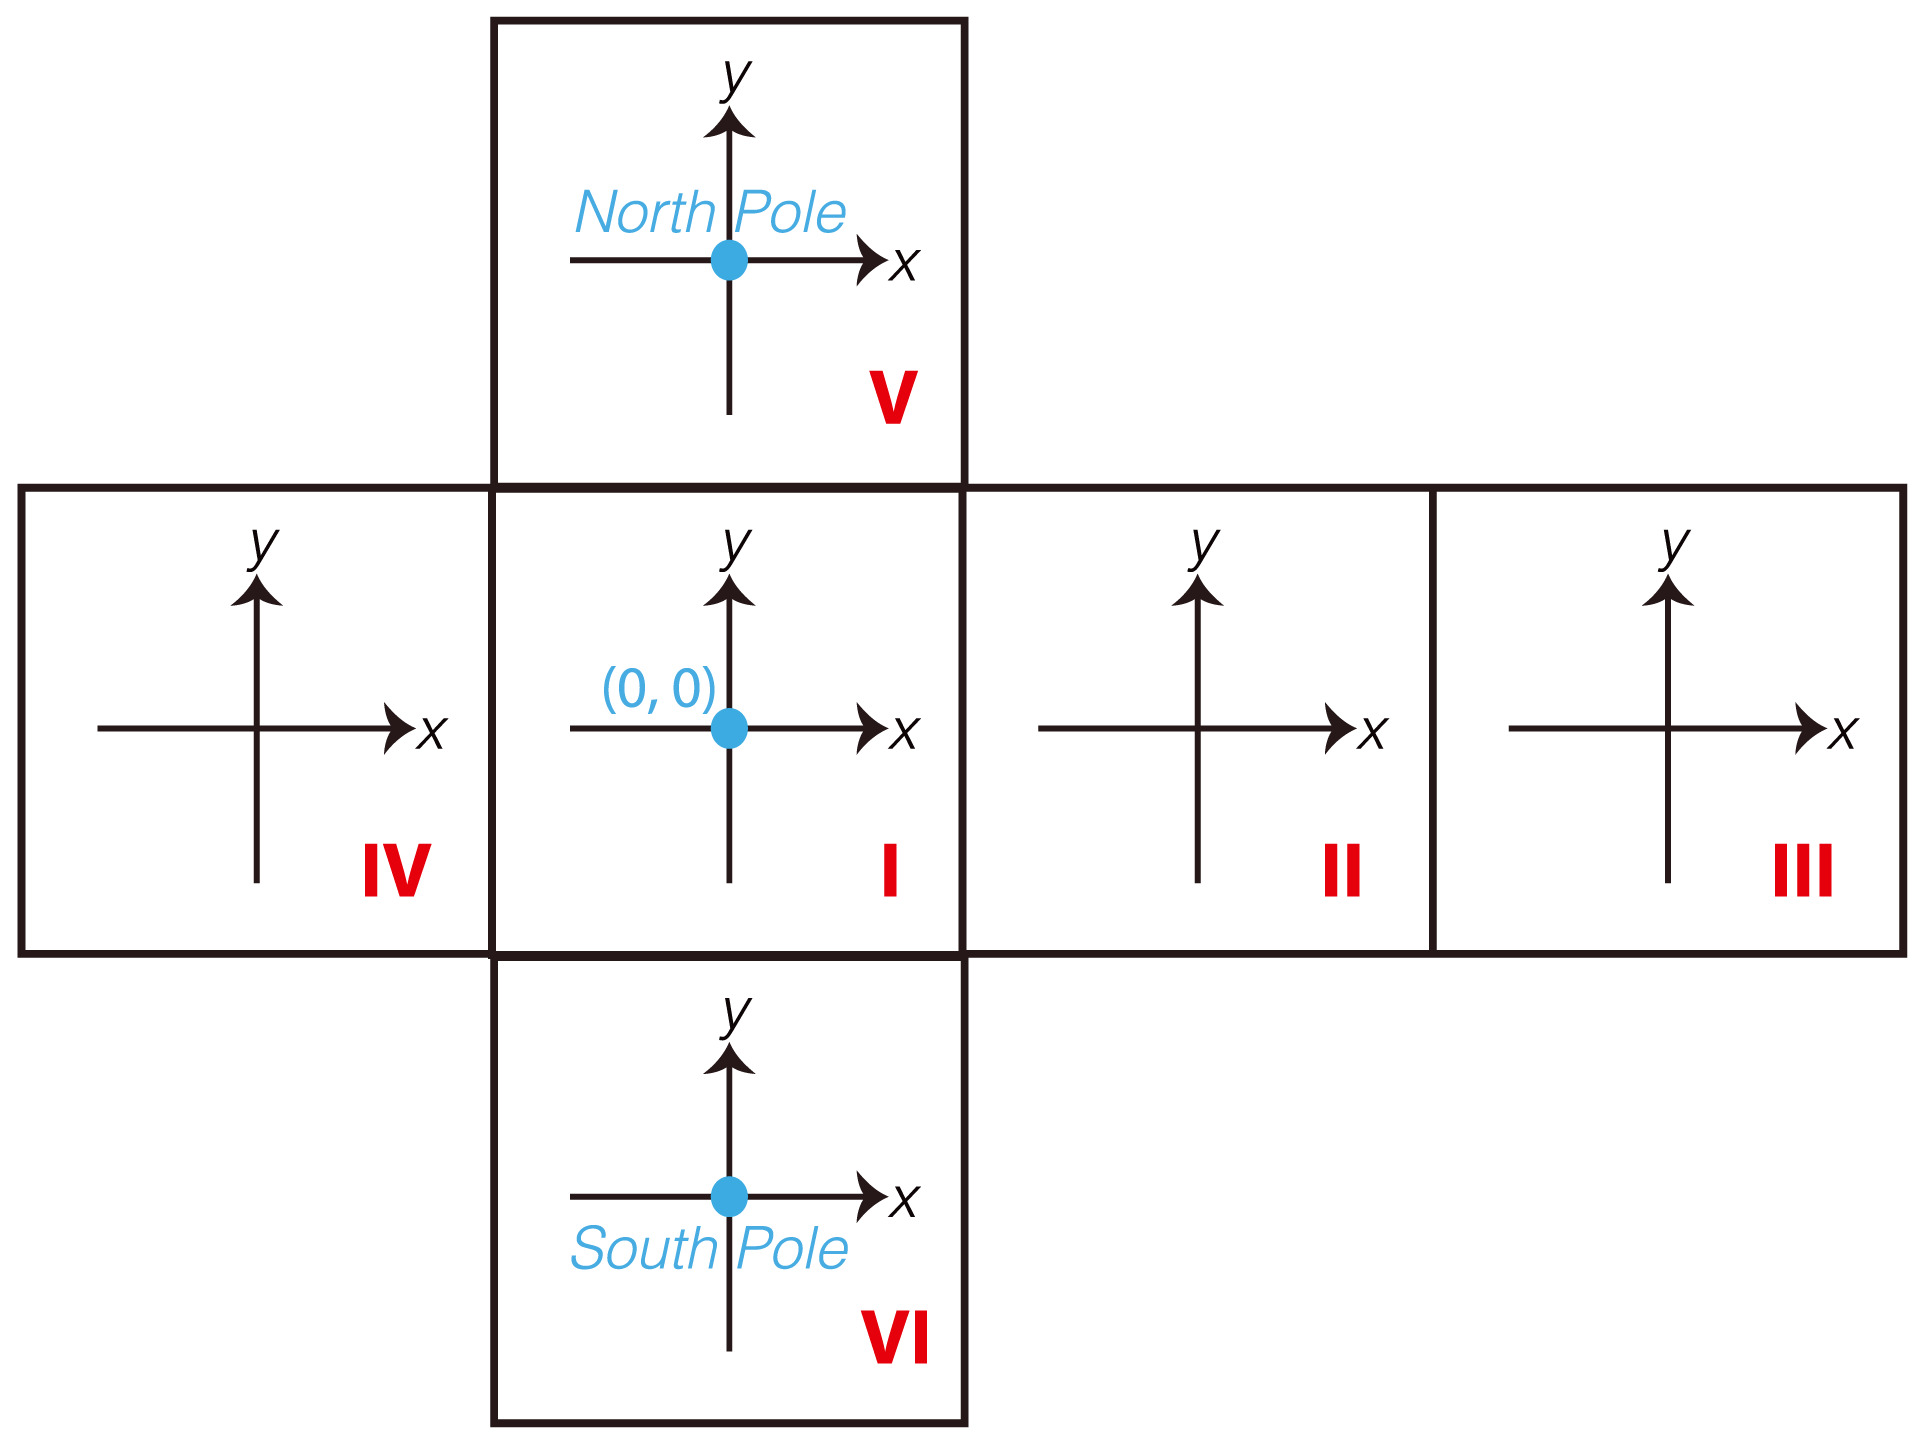
\includegraphics[width=0.4\linewidth]{chp4_panels}
	\caption{Cubed-sphere panels definition and orientation.
    Figure taken from \citet{jung:2019}.\label{chp-cs-panels}}
\end{figure}

The derivative of the maps $\boldsymbol{\Gamma}_p$ are given by:
\begin{equation*}
	d\boldsymbol{\Gamma}_{1}(x,y) = \frac{R}{{(1 + x^2 + y^2)}^{3/2}}
	\begin{bmatrix}
		-x & -y \\
	 	 1+y^2  & -xy \\
		 -xy  & 1+x^2
	\end{bmatrix}, \quad
	d\boldsymbol{\Gamma}_{2}(x,y) = \frac{R}{{(1 + x^2 + y^2)}^{3/2}}
	\begin{bmatrix}
		-(1+y^2) & xy \\
		 -x &  -y \\
		 -xy &  1+x^2
	\end{bmatrix},
\end{equation*}
\begin{equation*}
	d\boldsymbol{\Gamma}_{3}(x,y) = \frac{R}{{(1 + x^2 + y^2)}^{3/2}}
	\begin{bmatrix}
		 x &  y \\
		-(1+y^2) & xy \\
		 -xy &  1+x^2
	\end{bmatrix}, \quad
	d\boldsymbol{\Gamma}_{4}(x,y) = \frac{R}{{(1 + x^2 + y^2)}^{3/2}}	
	\begin{bmatrix}
		 1+y^2 &  -xy \\
		 x & y \\
		 -xy &  1+x^2
	\end{bmatrix},
\end{equation*}
\begin{equation*}
	d\boldsymbol{\Gamma}_{5}(x,y) = \frac{R}{{(1 + x^2 + y^2)}^{3/2}}	
	\begin{bmatrix}
		 xy  & -(1+x^2) \\
	 	 1+y^2  &  -xy \\
		-x & -y
	\end{bmatrix}, \quad
	d\boldsymbol{\Gamma}_{6}(x,y) = \frac{R}{{(1 + x^2 + y^2)}^{3/2}}
	\begin{bmatrix}
		 -xy  &  1+x^2 \\
		 1+y^2  &  -xy \\
		 x &  y
	\end{bmatrix}.
\end{equation*}
With the aid of the derivative, we may define a basis of tangent vectors 
$\{{\partial_x \boldsymbol{\Gamma}},  {\partial_y \boldsymbol{\Gamma}}\}$ on each point on the sphere by:
\begin{equation*}
	{\partial_x \boldsymbol{\boldsymbol{\Gamma}}}(x,y,p) = d\boldsymbol{\boldsymbol{\Gamma}}_{p}(x,y) \cdot
	\begin{bmatrix}
		 1 \\
		 0
	\end{bmatrix}, \quad
	{\partial_y \boldsymbol{\boldsymbol{\Gamma}}}(x,y,p) = d\boldsymbol{\boldsymbol{\Gamma}}_{p}(x,y) \cdot
	\begin{bmatrix}
		 0 \\
		 1
	\end{bmatrix}.
\end{equation*}
Notice that the matrix
\begin{equation*}
	\label{chp-cs-eqdistant-Gammatensor}
	G_{\boldsymbol{\Gamma}}(x,y) := 
	[d\boldsymbol{\Gamma}_{p}(x,y)]^Td\boldsymbol{\Gamma}_{p}(x,y)
	= \frac{R^2}{(1 + x^2 + y^2)^2}
	\begin{bmatrix}
		  1+ x^2 &  -xy \\
		 -xy & 1 + y^2
	\end{bmatrix},
\end{equation*}
does not depend on $p$.
This matrix is known as metric tensor.
It is easy to see that:
\begin{equation}
	\label{chp-cs-eqdistant-Gamma-metric-tensor}
	G_{\boldsymbol{\Gamma}}(x,y) = 
	\begin{bmatrix}
		\langle  {\partial_x \boldsymbol{\Gamma}_p}, {\partial_x  \boldsymbol{\Gamma}_p} \rangle & 
		\langle  {\partial_x \boldsymbol{\Gamma}_p}, {\partial_y  \boldsymbol{\Gamma}_p} \rangle \\
		\langle  {\partial_x  \boldsymbol{\Gamma}_p}, {\partial_y  \boldsymbol{\Gamma}_p} \rangle  &
		\langle  {\partial_y  \boldsymbol{\Gamma}_p}, {\partial_y  \boldsymbol{\Gamma}_p} \rangle 
	\end{bmatrix},
\end{equation}
where $\langle \cdot, \cdot \rangle$ denotes 
the standard inner product of $\mathbb{R}^3$,
and that $G_{\Gamma}(x,y)$ is positive-definite, 
$\forall (x,y) \in [-1,1]\times[-1,1]$.
The Jacobian of the metric tensor $G_{\boldsymbol{\Gamma}}(x,y)$, denoted by $\sqrt{\mathfrak{g}_{\boldsymbol{\Gamma}}}$ and called metric term, is then given by:
\begin{equation*}
        \sqrt{\mathfrak{g}_{\boldsymbol{\Gamma}}}(x,y) :=
	\sqrt{|\det{G_{\boldsymbol{\Gamma}}(x,y)}|} = \frac{R^2}{(1+x^2+y^2)^{3/2}}.
\end{equation*}
Now let us assume that we have a function $\beta:[-\alpha,\alpha] \to [-1,1]$, for some positive $\alpha>0$,
supposed to be bijective and $\mathcal{C}^1$ with inverse $\mathcal{C}^1$ as well.
That is, $\beta$ is a change of coordinates.
Let us consider $ \boldsymbol{\Psi}_p: [-\alpha,\alpha]\times [-\alpha,\alpha] \to \mathbb{S}^2_R$,
given by 
\begin{equation*}
	\boldsymbol{\Psi}_p(x,y) := \boldsymbol{\Gamma}_p\big(\beta(x),\beta(y)\big).
\end{equation*}
It follows from the chain rule that:
\begin{equation*}
        d \boldsymbol{\Psi}_p(x,y) = d \boldsymbol{\Gamma}_p\big(\beta(x),\beta(y)\big)\cdot\text{diag}\big(\beta'(x),\beta'(y)\big),
\end{equation*}
where $\text{diag}(\beta'(x),\beta'(y))$ is a diagonal $2\times 2$ matrix with diagonal entries given by $\beta'(x)$ and $\beta'(y)$.
We also have that tangent vector basis $\{{\partial_x  \boldsymbol{\Psi}_p},  {\partial_y  \boldsymbol{\Psi}_p}\}$ satisfying
\begin{align*}
	{\partial_x  \boldsymbol{\Psi}_p}(x,y) = \beta'(x) \cdot {\partial_x  \boldsymbol{\Gamma}_p}\big(\beta(x),\beta(y)\big),\\
	{\partial_y  \boldsymbol{\Psi}_p}(x,y) = \beta'(y) \cdot {\partial_y  \boldsymbol{\Gamma}_p}\big(\beta(x),\beta(y)\big).
\end{align*}
The metric tensor of $\boldsymbol{\Psi}_p$ is defined as $G_{\Gamma}$ in Equation \eqref{chp-cs-eqdistant-Gamma-metric-tensor}:
\begin{equation*}
	\label{chp-cs-eqdistant-Psi-metric-tensor}
	G(x,y) = 
	\begin{bmatrix}
		\langle  {\partial_x  \boldsymbol{\Psi}_p}, {\partial_x \boldsymbol{\Psi}_p} \rangle & 
		\langle  {\partial_x  \boldsymbol{\Psi}_p}, {\partial_y \boldsymbol{\Psi}_p} \rangle \\
		\langle  {\partial_x  \boldsymbol{\Psi}_p}, {\partial_y \boldsymbol{\Psi}_p} \rangle  &
		\langle  {\partial_y  \boldsymbol{\Psi}_p}, {\partial_y \boldsymbol{\Psi}_p} \rangle 
	\end{bmatrix}.
\end{equation*}
Finally, the metric term $\sqrt{\mathfrak{g}}:= \sqrt{\det{G}}$ is expressed in terms of $\sqrt{\mathfrak{g}}_{\Gamma}$ as
\begin{align*}
    \sqrt{\mathfrak{g}}(x,y) &= \beta'(x)\beta'(y)\sqrt{\mathfrak{g}}_{\Gamma}\big(\beta(x),\beta(y)\big)\\
    &= \beta'(x)\beta'(y)\frac{R^2}{\big(1+\beta(x)^2+\beta(y)^2\big)^{3/2}},
\end{align*}
which may also be expressed as
\begin{equation}
	\label{mt-sina}
	\sqrt{\mathfrak{g}}(x,y) =	
\|\partial_x  \boldsymbol{\Psi}_p \| \|\partial_y  \boldsymbol{\Psi}_p \| \sin \alpha(x,y,p),
\end{equation}
where $\alpha$ is the angle between $\partial_x \boldsymbol{\Psi}_p$ and $\partial_y \boldsymbol{\Psi}_p$ that
satisfies
\begin{equation*}
	\label{mt-cosa}
\cos{\alpha(x,y,p)} = \frac{\langle  {\partial_x  \boldsymbol{\Psi}_p}, {\partial_x \boldsymbol{\Psi}_p} \rangle }
{\|\partial_x \boldsymbol{\Psi}_p\|  \|\partial_y \boldsymbol{\Psi}_p\|}.
\end{equation*}

\newpage
\section{Cubed-sphere grids}
\label{sec-cs-grids}
Now that we have established the mapping between the cube and sphere with coordinate changes,
we may introduce the cubed-sphere grids proposed in the literature.

\subsection{Equidistant cubed-sphere}
\label{cs-equidistant}
The first cubed-sphere grid was proposed by \citet{sadourny:1972}. This grid is obtained by using
$\beta(x) = x$, $\alpha=1$ in the $\boldsymbol{\Psi}_p$ mapping described in Section \ref{equidistant-cs}.
This grid partitions the cube face into equally spaced points
and projects them onto the sphere, as illustrated in Figure
\ref{chp-cs-equidistant}, hence the name equidistant.
We shall denote this grid by \textbf{g1} since the parameter
\textbf{grid\_type} in FV3 is set equal to 1 to use this grid.

\subsection{Equiangular cubed-sphere}
\label{cs-equiangular}
Another cubed-sphere mapping is the equiangular mapping, 
introduced by \citet{ronchi:1996}, which leads to a more uniform grid.
This grid is obtained by considering the mapping $\boldsymbol{\Psi}_p$ described in Section \ref{equidistant-cs}
with $\beta(x) = \tan{x}$ and $\alpha=\frac{\pi}{4}$.
In this case, $\beta(x)$ represents the angular coordinates, and the cube-sphere is obtained by partitioning the angle between
grid points equally, as illustrated in Figure \ref{chp-cs-equiangular}, hence the name equiangular.
This grid is denoted by \textbf{g2}, for the same reason of the notation \textbf{g1}.
\begin{figure}[!htb]
	\centering
	\begin{subfigure}{0.42\textwidth}
		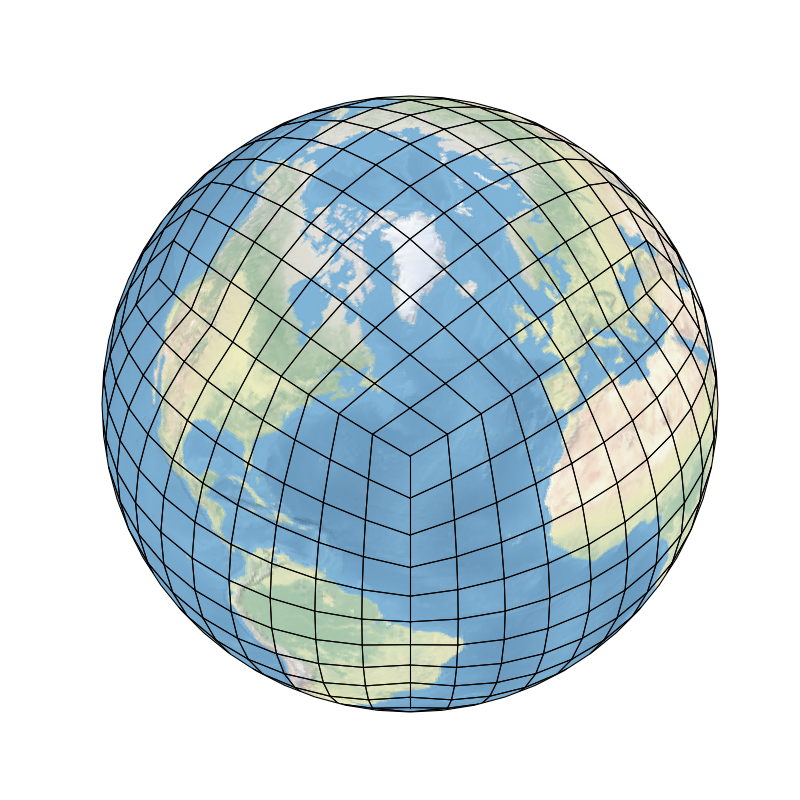
\includegraphics[width=1\linewidth]{gnomonic_equiangular_cs_10_sphere}
		\caption{Gridlines of the cube to the sphere equiangular mapping}
	\end{subfigure}
	\begin{subfigure}{0.42\textwidth}
		\centering
		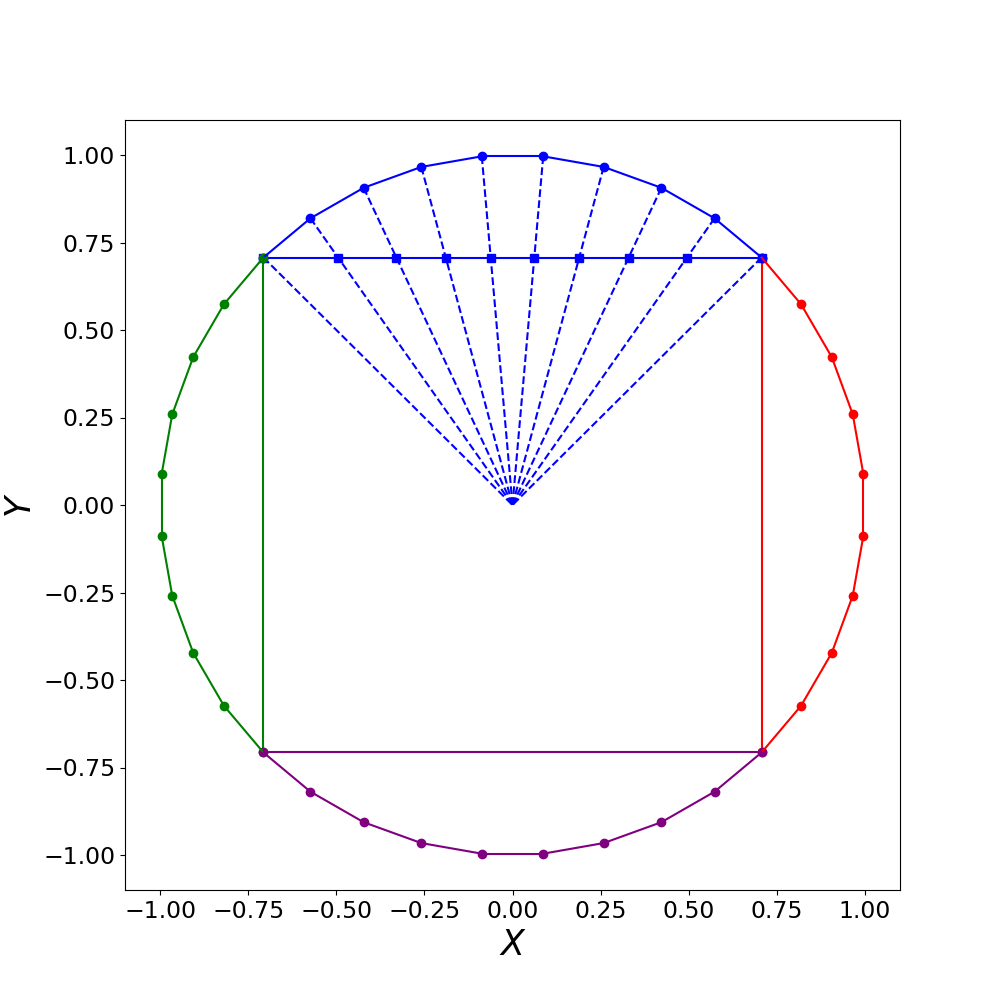
\includegraphics[width=1\linewidth]{g2}
		\caption{Cube and sphere equiangular mapping for $Z=0$.}
	\end{subfigure}
	\caption{(a) Illustration of the resulting cube-to-sphere mapping and (b) illustration of the cube-to-sphere projection using the equiangular mapping.\label{chp-cs-equiangular}}
\end{figure}

\subsection{Equi-edge cubed-sphere}
\label{cs-equiedge}
Another cubed-sphere mapping is the equi-edge proposed by
\citet{chen:2021} using $\beta(x) = \sqrt{2}\tan{x}$ and
$\alpha=\arcsin{\big(\frac{1}{\sqrt{3}}\big)}$.
Figure \ref{chp-cs-equiedge} illustrates the equi-edge mapping.
\begin{figure}[!htb]
	\centering
	\begin{subfigure}{0.42\textwidth}
		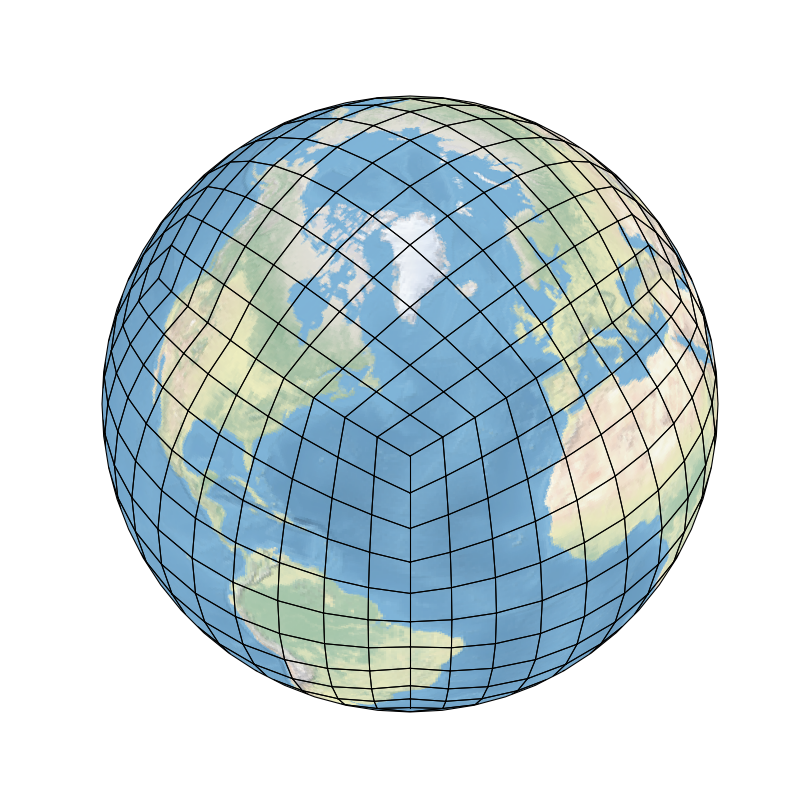
\includegraphics[width=1\linewidth]{gnomonic_equiedge_cs_10_sphere}
		\caption{Gridlines of the cube to the sphere equi-edge mapping}
	\end{subfigure}
	\begin{subfigure}{0.42\textwidth}
		\centering
		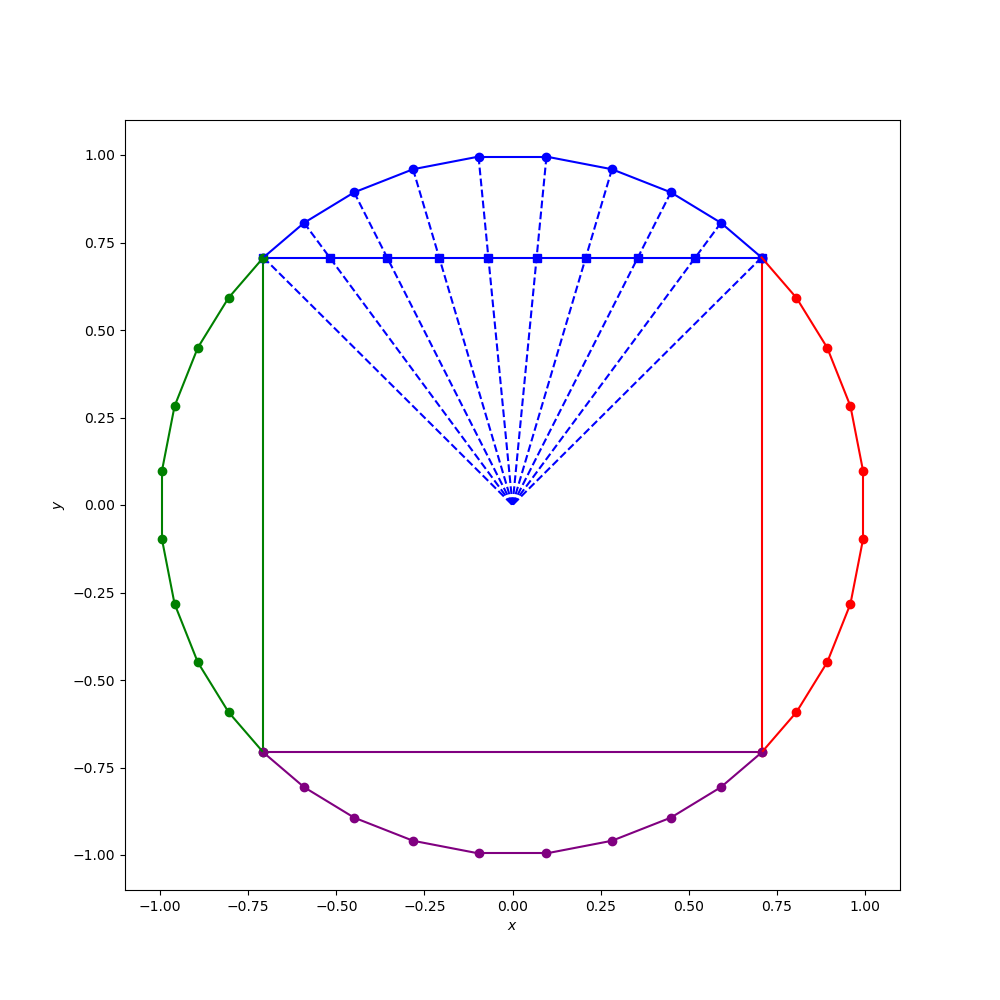
\includegraphics[width=1\linewidth]{g0}
		\caption{Cube and sphere equi-edge mapping for $Z=0$.}
	\end{subfigure}
	\caption{(a) Illustration of the resulting cube-to-sphere mapping and (b) illustration of the cube-to-sphere projection using the equi-edge mapping.\label{chp-cs-equiedge}}
\end{figure}

The idea behind the equi-edge cubed-sphere lies in partitioning the edges of the spherical cube equally,
and then generating the other cells, hence the name equi-edge.
This grid is denoted by \textbf{g0}, for the same reason of the notation \textbf{g1}.
Also, this grid leads to more uniform cells after applying the grid stretching option of FV3 \citep{harris:2016, chen:2021}.

\subsection{Geometric properties}
\label{cs-geo}
We will utilize the notation introduced in Section \ref{chp-adv2d-sec-not} throughout this Chapter.
We shall used the Earth radius $R = 6.371 \times 10^6$ meters.
The parameter $\nu$ represents a non-negative integer indicating the number of ghost cell layers in each panel boundary, called halo size.
To generate the cubed-sphere, we consider a $(\Delta x, \Delta y)$-grid denoted by 
$\Omega_{\Delta x, \Delta y} = (\Omega_{ij})_{i,j=-\nu+1,\ldots,N+\nu}$, 
where $\Delta x = \Delta y$, and it covers the domain $\Omega$. 
A control volume of the cubed-sphere is denoted by $\Omega_{ijp}$, defined as follows:
\begin{equation*}
	\Omega_{ijp} = \Psi_p(\Omega_{ij})
	\quad -\nu+1 \leq i, j \leq N+\nu, \quad 1 \leq p \leq 6.
\end{equation*}
The cubed-sphere grid refers to the collection of control volumes 
$(\Omega_{ijp})_{i,j=-\nu+1,\ldots,N+\nu}^{p=1,\ldots,6}$. 
In Figures \ref{chp-cs-equidistant}, \ref{chp-cs-equiangular} and \ref{chp-cs-equiedge} examples of the cubed-sphere grids are depicted,
excluding the ghost cells.
These grids are generated using the equidistant, equiangular and equi-edge mappings for $N=10$.

We will denote the area of $\Omega_{ijp}$ by $|\Omega_{ij}|$.
Notice that the area does not depend on the panel due to the grid symmetry.
We also define the diameter of a cell as $2\sqrt{\frac{|\Omega_{ij}|}{\pi}}$, which corresponds to the diameter of a circle with area $|\Omega_{ij}|$.
This gives a good approximation to the cell diameters, as a cell on the cubed-sphere has similar lengths.
The control volume area is given by:
\begin{equation}
	\label{chp4-area}
	|\Omega_{ij}| = \int_{x_{i-\frac{1}{2}}}^{x_{i+\frac{1}{2}}} \int_{y_{j-\frac{1}{2}}}^{y_{j+\frac{1}{2}}}{\sqrt{\mathfrak{g}}(x,y)} \,dx \,dy = 
	|\hat{\Omega}_{ij}| + \mathcal{O}(\Delta x^2),
\end{equation}
where $|\hat{\Omega}_{ij}| = \sqrt{\mathfrak{g}}(x_i,y_j) \Delta x \Delta y$,
and the last equality follows from Proposition \ref{prop-bound-centroid-2d}.
In tables \ref{g0-dx-table}, \ref{g1-dx-table}, and \ref{g2-dx-table},
we display the diameters of the  equi-edge (g0), equidistant (g1), and equiangular (g2) grids for $N=48\times 2^k$, 
where $k = 0,\ldots, 4$. These values of $N$ are considered in this work.
Similarly, in tables \ref{g0-da-table}, \ref{g1-da-table}, and \ref{g2-da-table}, we display the areas.


\begin{table}[htbp]
    \centering
    \caption{Mean diameter, minimum diameter, and maximum diameter for different values of $N$ considering the equi-edge grid (g0).\label{g0-dx-table}}
    \begin{tabular}{cccccc}
        \toprule
        $N$ & Mean Length (km) & Min Length (km) & Max Length (km) & $\frac{\text{Max}}{\text{Min}}$ \\
        \midrule
        48 & 218 & 175 & 266 & 1.5192 \\
        96 & 108 & 86 & 131 & 1.5195 \\
        192 & 54 & 43 & 65 & 1.5196 \\
        384 & 26 & 21 & 32 & 1.5197 \\
        768 & 13 & 10 & 16 & 1.5197 \\
        \bottomrule
    \end{tabular}
\end{table}

\begin{table}[htbp]
    \centering
    \caption{As Table \ref{g0-dx-table} but considering the equidistant grid (g1). \label{g1-dx-table}}
    \begin{tabular}{cccccc}
        \toprule
        $N$ & Mean Length (km) & Min Length (km) & Max Length (km) & $\frac{\text{Max}}{\text{Min}}$ \\
        \midrule
        48 & 215 & 134 & 305 & 2.2780 \\
        96 & 107 & 66 & 151 & 2.2791 \\
        192 & 53 & 33 & 75 & 2.2794 \\
        384 & 26 & 16 & 37 & 2.2795 \\
        768 & 13 & 8 & 18 & 2.2795 \\
        \bottomrule
    \end{tabular}
\end{table}

\begin{table}[htbp]
    \centering
    \caption{As Table \ref{g0-dx-table} but considering the equiangular grid (g2). \label{g2-dx-table}}
    \begin{tabular}{cccccc}
        \toprule
        $N$ & Mean Length (km) & Min Length (km) & Max Length (km) & $\frac{\text{Max}}{\text{Min}}$ \\
        \midrule
        48 & 220 & 202 & 240 & 1.1890 \\
        96 & 109 & 99 & 118  & 1.1892 \\
        192 & 54 & 49 & 59  & 1.1892 \\
        384 & 27 & 24 & 29  & 1.1892 \\
        768 & 13 & 12 & 14  & 1.1892 \\
        \bottomrule
    \end{tabular}
\end{table}


\begin{table}[htbp]
    \centering
    \caption{Mean area, minimum area, and maximum area for different values of $N$ considering the equi-edge grid (g0).\label{g0-da-table}}
    \begin{tabular}{cccccc}
        \toprule
        $N$ & Mean Area (km$^2$) & Min Area (km$^2$) & Max Area (km$^2$) & $\frac{\text{Max}}{\text{Min}}$ \\
        \midrule
        48 & 38033 & 24113 & 55650 & 2.3078 \\
        96 & 9364 & 5902 & 13628 & 2.3090 \\
        192 & 2323 & 1460 & 3371 & 2.3093 \\
        384 & 578 & 363 & 838 & 2.3094 \\
        768 & 144 & 90 & 209 & 2.3094 \\
        \bottomrule
    \end{tabular}
\end{table}

\begin{table}[htbp]
    \centering
    \caption{As Table \ref{g0-da-table} but considering the equidistant grid (g1). \label{g1-da-table}}
    \begin{tabular}{cccccc}
        \toprule
        $N$ & Mean Area (km$^2$) & Min Area (km$^2$) & Max Area (km$^2$) & $\frac{\text{Max}}{\text{Min}}$ \\
        \midrule
        48 & 37762 & 14145 & 73403 & 5.1891 \\
        96 & 9331 & 3462 & 17985 & 5.1944 \\
        192 & 2319 & 856 & 4450 & 5.1957 \\
        384 & 578 & 213 & 1106 & 5.1960 \\
        768 & 144 & 53 & 276 & 5.1961 \\
        \bottomrule
    \end{tabular}
\end{table}

\begin{table}[htbp]
    \centering
    \caption{As Table \ref{g0-da-table} but considering the equiangular grid (g2). \label{g2-da-table}}
    \begin{tabular}{cccccc}
        \toprule
        $N$ & Mean Area (km$^2$) & Min Area (km$^2$) & Max Area (km$^2$) & $\frac{\text{Max}}{\text{Min}}$ \\
        \midrule
        48 & 38269 & 32062 & 45327 & 1.4137 \\
        96 & 9393 & 7847 & 11096 & 1.4141 \\
        192 & 2327 & 1941 & 2745 & 1.4142 \\
        384 & 579 & 482 & 682 & 1.4142 \\
        768 & 144 & 120 & 170 & 1.4142 \\
        \bottomrule
    \end{tabular}
\end{table}


We can observe that in terms of areas and diameters of the cells, the equidistant grid (g1) is the less uniform,
while the equiangular grid  is the most uniform grid.
The equi-edge grid is more uniform than the equidistant grid, but the maximum/minimum ratio of the areas is almost 2.3. 
Despite this, the equi-edge grid is the operational grid in some applications of FV3 \citep{harris:2021,chen:2021}, such as, for instance, 
the Next Generation Global Prediction System (NGGPS) \citep{zhou:2019}, 
because this grid is expected to produce less grid imprinting due to its greater uniformity near the cubed edges.
Therefore, in this thesis, we shall constrain our attention only to the  equi-edge and equiangular grids, since the equiangular grid is ideally more uniform and the equi-edge grid  is currently used in FV3.
In Figure \ref{chp-cs-areas}, we illustrate the areas of both grids, equi-edge (g0) and equiangular (g2).
We can observe that the areas of the equi-edge grid exhibit a higher gradient near the cube corners, while the equiangular grid appears to have a higher gradient near the middle of the cube edges.
\begin{figure}[!htb]
	\centering
	\begin{subfigure}{0.48\textwidth}
		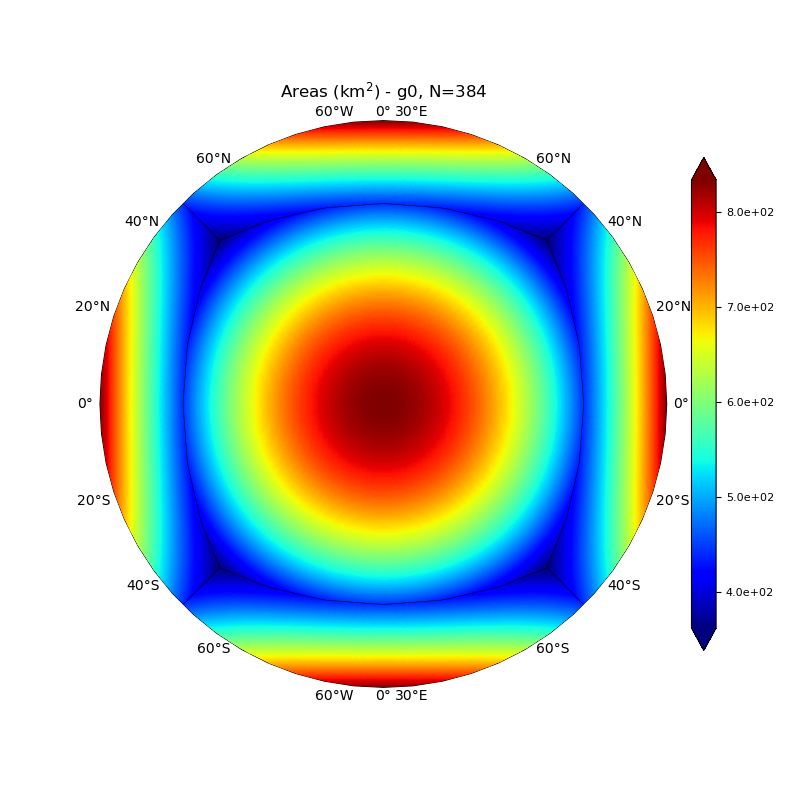
\includegraphics[width=0.8\linewidth]{g0_384}
		\caption{g0 grid areas (km$^2$).}
	\end{subfigure}
	\begin{subfigure}{0.48\textwidth}
		\centering
		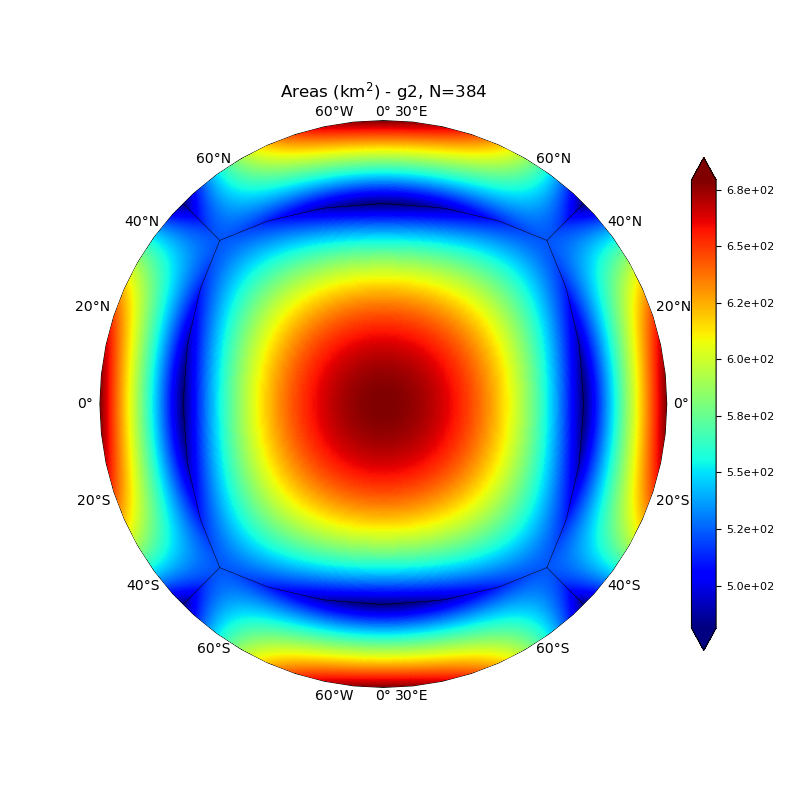
\includegraphics[width=0.8\linewidth]{g2_384}
		\caption{g2 grid areas (km$^2$).}
	\end{subfigure}
	\caption{Areas for the grid equi-edge (g0) and equiangular grid (g2) using $N=384$.\label{chp-cs-areas}}
\end{figure}

There are four types of grid points on the cubed-sphere that we need to compute: the center, corners, right-left edge midpoints, and  up-down edge midpoints.
The locations of these points are illustrated in Figure \ref{chp-cs-gridpoints} for the equiangular grid (g2).
\begin{figure}[!htb]
	\centering
	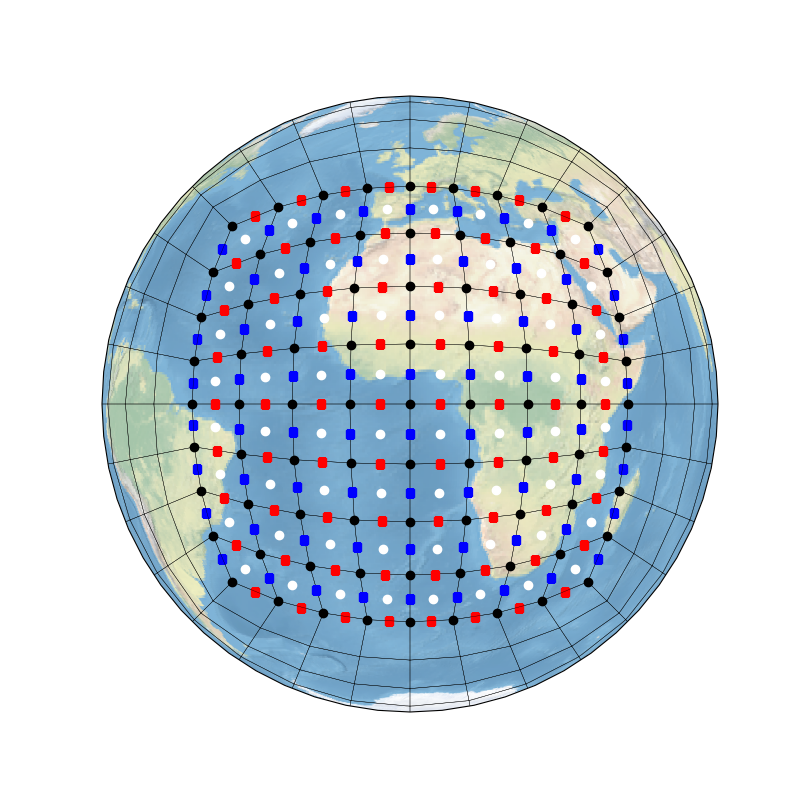
\includegraphics[width=0.5\linewidth]{gridpoints_sphere}
	\caption{Illustration of the center (white), corner (black), right-left edge (blue) and up-down edge (red) points 
		for the equiangular grid (g2) with $N=10$.\label{chp-cs-gridpoints}}
\end{figure}

One possible approach is to use the cubed-sphere mapping to generate these points, based on the grid points projected onto the sphere from the plane.
These points shall be denoted using a superscript 'c'.
The corner points, as the name suggest, represent the corners of the control volume, namely
\begin{equation}
	\Psi_{i+\frac{1}{2},j+\frac{1}{2},p}^c := \Psi_p(x_{i+\frac{1}{2}},y_{j+\frac{1}{2}}).
\end{equation}
Similarly, the cell centers are:
\begin{equation}
	\Psi_{ijp}^c := \Psi_p(x_{i},y_{j}).
\end{equation}
The right-left edge points are the midpoints of the edge in the $y$-direction, namely:
\begin{equation}
	\Psi_{i+\frac{1}{2},j,p}^c := \Psi_p(x_{i+\frac{1}{2}},y_{j}).
\end{equation}
The up-down edge points are the midpoints of the edge in the $x$-direction, namely:
\begin{equation}
	\Psi_{i,j+\frac{1}{2},p}^c := \Psi_p(x_{i},y_{j+\frac{1}{2}}).
\end{equation}
The grids equi-edge (g0) and equiangular (g2), formulated with these grid points, are denoted by \textbf{g0.c} and \textbf{g2.c}, respectively.
We refer to this grid point formulation as cube midpoints, which is a common approach used in the literature \citep{guo:2014,katta:2015,katta:2015b,nair:2005,ullrich:2016}.

Another way to compute the grid points, which is used in FV3, is to compute the corner
points as before and obtain the center, right-left edge and up-down edge points using the spherical midpoints.
These points shall be denoted using a superscript 's'.
The corner points in this case are:
\begin{equation}
	\Psi_{i+\frac{1}{2},j+\frac{1}{2},p}^s := \Psi_{i+\frac{1}{2},j+\frac{1}{2},p}^c.
\end{equation}
The center points are computed by averaging the values of 4 corner points:
\begin{equation}
	\Psi_{ijp}^s :=
	\frac{\Psi_{i+\frac{1}{2},j+\frac{1}{2},p}^s + \Psi_{i+\frac{1}{2},j-\frac{1}{2},p}^s + \Psi_{i-\frac{1}{2},j+\frac{1}{2},p}^s + \Psi_{i-\frac{1}{2},j-\frac{1}{2},p}^s}
         {\|\Psi_{i+\frac{1}{2},j+\frac{1}{2},p}^s + \Psi_{i+\frac{1}{2},j-\frac{1}{2},p}^s + \Psi_{i-\frac{1}{2},j+\frac{1}{2},p}^s + \Psi_{i-\frac{1}{2},j-\frac{1}{2},p}^s\|}.
\end{equation}
Similarly, the right-left edge points are obtained by averaging the values of 2 corner points.
\begin{equation}
	\Psi_{i+\frac{1}{2},j,p}^s :=
	\frac{\Psi_{i+\frac{1}{2},j+\frac{1}{2},p}^s + \Psi_{i+\frac{1}{2},j-\frac{1}{2},p}^s}
	   {\|\Psi_{i+\frac{1}{2},j+\frac{1}{2},p}^s + \Psi_{i+\frac{1}{2},j-\frac{1}{2},p}^s\|}.
\end{equation}
and the up-down edge points are also  given by the average  the values of 2 corner points:
\begin{equation}
	\Psi_{i,j+\frac{1}{2},p}^s :=
	\frac{\Psi_{i+\frac{1}{2},j+\frac{1}{2},p}^s + \Psi_{i-\frac{1}{2},j+\frac{1}{2},p}^s}
	     {\|\Psi_{i+\frac{1}{2},j+\frac{1}{2},p}^s + \Psi_{i-\frac{1}{2},j+\frac{1}{2},p}^s\|}.
\end{equation}
The grids equi-edge (g0) and equiangular (g2), formulated with these grid points, are denoted by \textbf{g0.s} and \textbf{g2.s}, respectively.
We refer to this grid points formulation as spherical midpoints.
One can easily see that:
\begin{align}
	\Psi_{i+\frac{1}{2},j,p}^s &= \Psi_{i+\frac{1}{2},j,p}^c+ \mathcal{O}(\Delta x^2),\\
	\Psi_{i,j+\frac{1}{2},p}^s &= \Psi_{i,j+\frac{1}{2},p}^c+ \mathcal{O}(\Delta x^2),\\
	\Psi_{i,j,p}^s &= \Psi_{i,j,p}^c + \mathcal{O}(\Delta x^2).
\end{align}
Then, we should expect similar results when using different grid point formulations, especially when using a high-resolution grid.
In g0.c or g2.c grids, the points are aligned along geodesics.
This happens because the cube-mapping maps lines on the plane onto geodesics on the sphere.
However, one can see that this does not occur on g0.s or g2.s, as the center, right-left edge, and up-down edge points are not aligned on the same geodesic.
Although this misalignment becomes negligible for high resolutions,
it impacts ghost cell interpolation accuracy, as we shall see in Section \ref{cs-halodata}.

Hereafter in this Subsection, we are going to omit the superscripts 's' and 'c', because what is described here has the same meaning for both midpoint formulations.
Finally, we introduce the following geodesic distances in $x$ and $y$ directions, respectively,
\begin{align}
	\label{distcube}
	{\delta} x_{ij} &= d(\Psi_{i+\frac{1}{2},j,p},\Psi_{i-\frac{1}{2},j,p}) ,\\
	{\delta} y_{ij} &= d(\Psi_{i,j+\frac{1}{2},p},\Psi_{i,j-\frac{1}{2},p}),
\end{align}
where $d(P,Q) = R\arccos{(\langle P, Q \rangle)}$, for $P,Q \in \mathbb{S}^2_R$, and we assume that $i$ and $j$ can be integers or half-integers.
Notice that these distances do not depend on the panel due to the grid symmetry.
These distances may be represented in terms of the tangent vector norms as:
\begin{align}
	{\delta} x_{ij} &= 
	\int_{x_{i-\frac{1}{2}}}^{x_{i+\frac{1}{2}}}
	\|\partial_x  \mathbf{\Psi}_{p}\|(x,y_j) \,dx ,\\
	{\delta} y_{ij} &=
	\int_{y_{j-\frac{1}{2}}}^{y_{j+\frac{1}{2}}}
	\|\partial_y \mathbf{\Psi}_{p}\|(x_i,y) \,dy.
\end{align}
Hence, their midpoint approximations are defined as:
\begin{align}
	\label{distcube2}
	\hat{\delta} x_{ij} &= \|\partial_x \mathbf{\Psi}_{ijp} \|\Delta x,\\
	\hat{\delta} y_{ij} &= \|\partial_y \mathbf{\Psi}_{ijp} \|\Delta y,
\end{align}
which are second-order accurate (see Theorem \ref{prop-bound-midpoint1d}):
\begin{align}
\delta x_{ij} = \hat{\delta} x_{ij} + \mathcal{O}(\Delta x^2),\\
\delta y_{ij} = \hat{\delta} y_{ij} + \mathcal{O}(\Delta y^2).
\end{align}
\subsection{Duo-grid points}
\label{duogrid-points}
The corner duo-grid points are generated by computing the mappings $\boldsymbol{\Psi}_p$ for the grid points 
$(x_{i+\frac{1}{2}}, y_{j+\frac{1}{2}})$ where $i$ and $j$ out of the range $0$ to $N$. 
When using the cube midpoint formulation, the center, right-left edge, and up-down edge points are computed analogously.
In Figure \ref{cs-duo}, we illustrate the duo-grid points obtained for both equi-edge and equiangular grids.
We can observe in Figure \ref{cs-duo-g2} that the corner duo-grid points of the equiangular grid are aligned on common geodesics.
This property has been known since the work of \citet{ronchi:1996}, and similarly, it holds for center, right-left edge, and up-down edge duo-grid points when using the cube midpoint formulation.
This property is very useful because it allows us to use 1D Lagrange interpolation to estimate the duo-grid values using values 
from neighboring panels, and it has been widely used in the literature \citep{ross:2006, croisille:2013,katta:2015,katta:2015b, chen:2021}.

However, it is evident from Figure \ref{cs-duo-g0} that the analogous property does not hold for the equi-edge grid
To address this problem, \citet{chen:2021} proposes modifying the ghost values of the $x$ and $y$ coordinates by mirroring certain points. 
This generates the new duo-grid points, aligning them on the same geodesic as those from the neighboring panel.
More formally, for $g=1,2,\ldots,\nu$, we introduce the mirrored values
\begin{align}
	\hat{x}_{-g+\frac{1}{2}}  &= \arctan\left(\frac{1}{\alpha}\tan\left(-\frac{\pi}{2}-\arctan{(\alpha \tan{x_{g+\frac{1}{2}} })}\right)\right),\\
	\hat{x}_{N+g+\frac{1}{2}} &= -\hat{x}_{-g+\frac{1}{2}}, \\
	\hat{y}_{-g+\frac{1}{2}}  &= \arctan\left(\frac{1}{\alpha}\tan\left(-\frac{\pi}{2}-\arctan{(\alpha \tan{y_{g+\frac{1}{2}} })}\right)\right),\\
	\hat{y}_{N+g+\frac{1}{2}} &= -\hat{y}_{-g+\frac{1}{2}},
\end{align}
to replace ${x}_{-g+\frac{1}{2}},{x}_{N+g+\frac{1}{2}},{y}_{-g+\frac{1}{2}}$ and ${y}_{N+g+\frac{1}{2}}$, respectively.
When computing the grid points using the cube midpoints formulation, the values of $x_i$ and $y_j$ are readjusted similarly.
Figure \ref{cs-duo-g02} illustrates how the modified duo-grid of equi-edge (g0) aligns with the geodesics of neighboring panels just as the equiangular grids (g2) (Figure \ref{cs-duo-g2}).
Notice, however, that the equi-edge corner points will no longer be equally spaced in terms of its $x$ and $y$ coordinates,
in contrast to equiangular grid, where the $x$ and $y$ coordinates of the corner points are uniformly spaced.
This may require special attention from numerical schemes using equi-edge near edges due to the loss of uniformity.
\begin{figure}[!htb]
	\centering
	\begin{subfigure}{0.45\textwidth}
		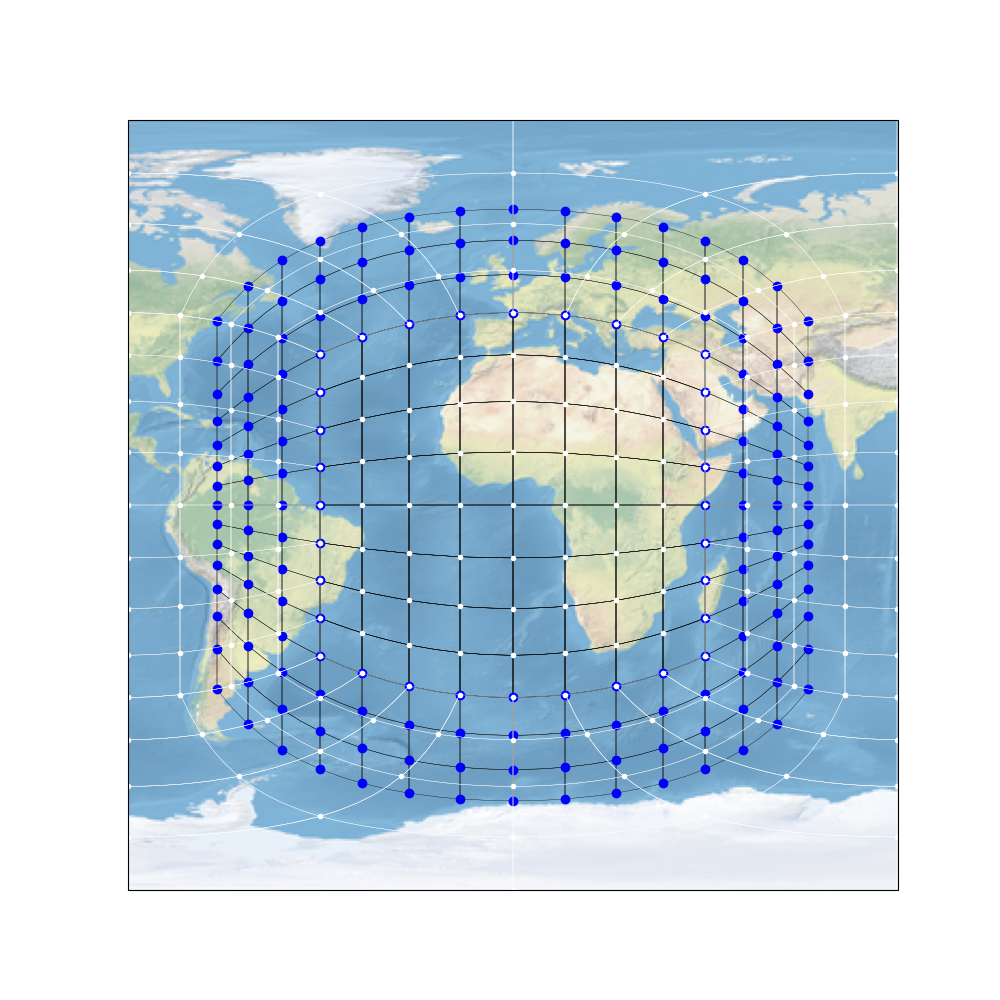
\includegraphics[width=1\linewidth]{g0_duo}
		\caption{g0 duo-grid.\label{cs-duo-g0}}
	\end{subfigure}
	\begin{subfigure}{0.45\textwidth}
		\centering
		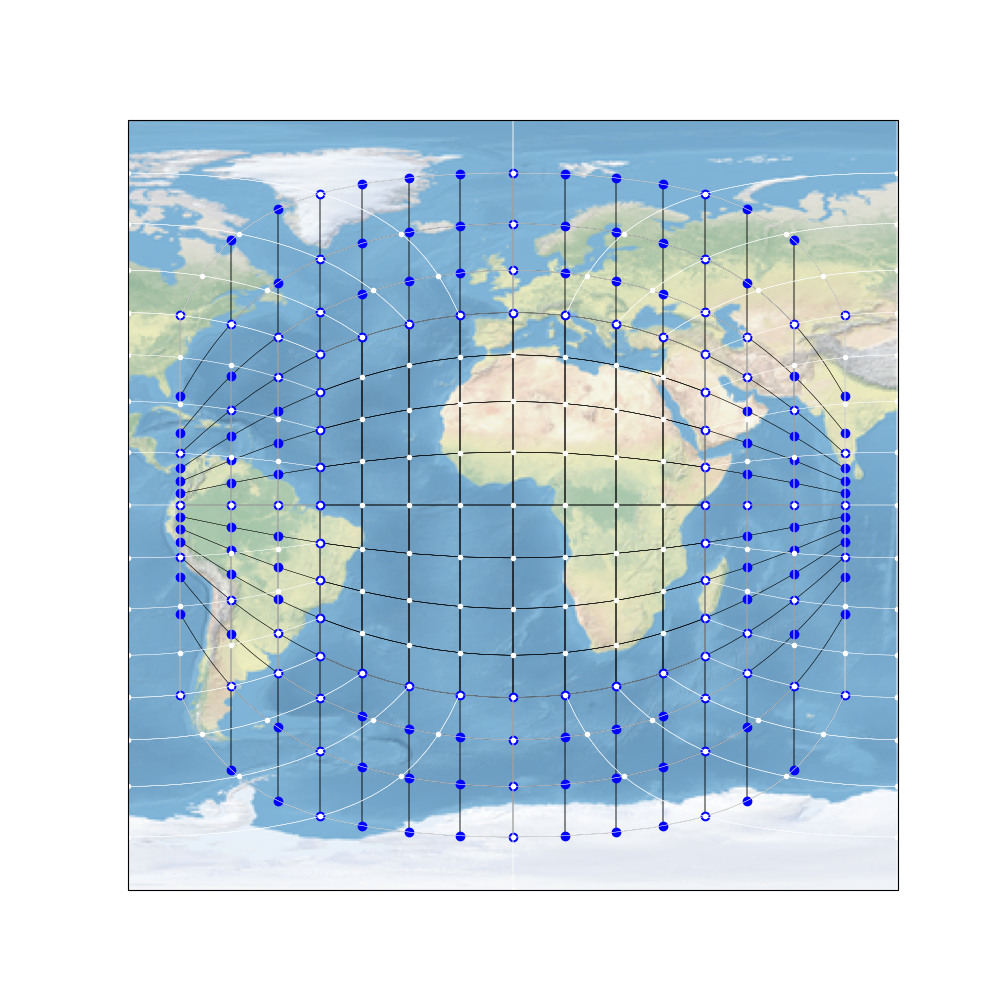
\includegraphics[width=1\linewidth]{g0_duo2}
		\caption{Mirrored g0 duo-grid.\label{cs-duo-g02}}
	\end{subfigure}
	\begin{subfigure}{0.45\textwidth}
		\centering
		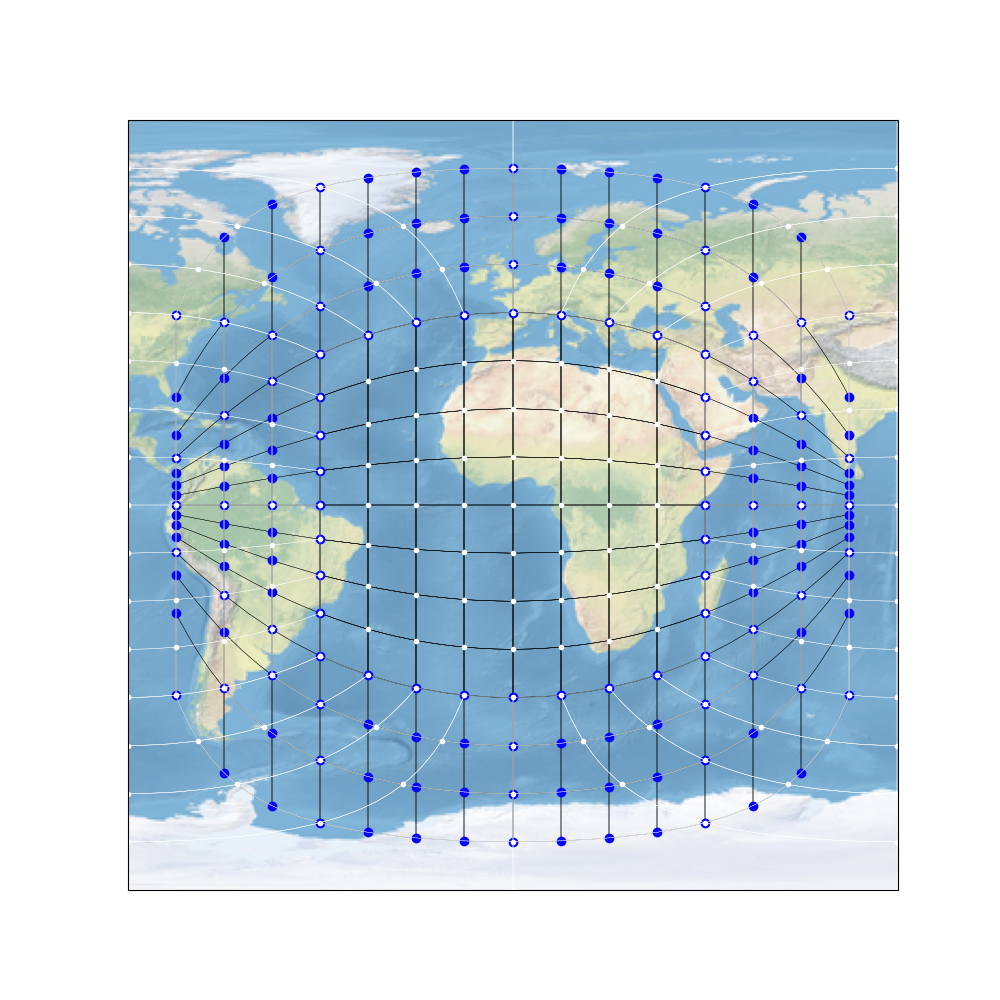
\includegraphics[width=1\linewidth]{g2_duo}
		\caption{g2 duo-grid.\label{cs-duo-g2}}
	\end{subfigure}
	\caption{Duo-grid lines of panel 1 for the equi-edge grid g0 (a) and the equiangular grid g2 (c). (b) shows the mirrored duo-grid of equi-edge grid.
		Corner duo-grid points are denoted by blue circles, and the corner points are denoted by white points.\label{cs-duo}}
\end{figure}

\subsection{Tangent vectors on the sphere}
\label{cs-tgvectors}
The tangent space at $P \in \mathbb{S}^2_R$ is denoted by $T_P \mathbb{S}^2$.
It is easy to see that:
\begin{equation*}
	T_P\mathbb{S}^2_R = \{P_0 \in \mathbb{R}^3: \langle P,P_0\rangle = 0\}.
\end{equation*}
We are going to consider three ways to represent an element of $\mathbb{S}_R^2$:
using $(X,Y,Z)$ coordinates, or using $(\lambda, \phi)$
latitude-longitude coordinates, or, at last, using the cubed-sphere
coordinates $(x,y,p)$, where $(x,y)$ are the cube face coordinates and 
$p \in \{1,2,\cdots, 6\}$ stands for a cube panel.
We say that a vector field $\boldsymbol{u}: \mathbb{S}^2_R \to 
\mathbb{R}^3$ is tangent on  the sphere if
$\boldsymbol{u}(P) \in T_P\mathbb{S}^2_R$, $\forall P \in \mathbb{S}^2_R$.

\subsubsection{Conversions between latitude-longitude and contravariant coordinates}
\label{anexo-sph-ll}
We consider the latitude-longitude mapping 
$\boldsymbol{\Pi}: [0,2\pi] \times [-\frac{\pi}{2},\frac{\pi}{2}] \to \mathbb{S}^2_R$, 
$\boldsymbol{\Pi} = ({\Pi}_1,{\Pi}_2,{\Pi}_3)$, given by:
\begin{align}
	\label{ll2sph}
	{\Pi}_1(\lambda,\phi) &= R\cos \phi \cos \lambda,\\
	{\Pi}_2(\lambda,\phi) &= R\cos \phi \sin \lambda,\\
	{\Pi}_3(\lambda,\phi) &= R\sin \phi.
\end{align}
The derivative or Jacobian matrix of the mapping $\boldsymbol{\Pi}$ is given by:
\begin{equation}
	\label{dGamma}
	d\boldsymbol{\Pi} (\lambda,\phi) = 
	R \begin{bmatrix}
		-\cos \phi \sin \lambda &  -\sin \phi \cos \lambda \\
		\cos \phi \cos \lambda & \sin \phi \sin \lambda \\
		0  &  \cos \phi
	\end{bmatrix}.
\end{equation}
Using this matrix's columns, we can define the tangent vectors:
\begin{equation}
	\partial_{\lambda}\boldsymbol{\Pi}(\lambda,\phi) = d\boldsymbol{\Pi}(\lambda,\phi)
	\begin{bmatrix}
		1 \\
		0
	\end{bmatrix}, \quad
	\partial_{\phi}\boldsymbol{\Pi}(\lambda,\phi) = d\boldsymbol{\Pi}(\lambda,\phi)
	\begin{bmatrix}
		0 \\
		1
	\end{bmatrix}.
\end{equation}
We normalize the vectors $\partial_{\lambda}\boldsymbol{\Pi}$ and $\partial_{\phi}\boldsymbol{\Pi}$
and we obtain unit tangent vectors on the sphere at $\Pi(\lambda, \phi)$:
\begin{equation}
	\label{latlon_tg_vectors}
	\boldsymbol{e}_{\lambda}(\lambda,\phi) = 
	\begin{bmatrix}
		-\sin \lambda \\
		\cos \lambda \\
		0
	\end{bmatrix}, \quad
	\boldsymbol{e}_{\phi}(\lambda,\phi) =
	\begin{bmatrix}
		-\sin \phi \cos \lambda \\
		-\sin \phi \sin \lambda \\
		\cos \phi
	\end{bmatrix}.
\end{equation}
Let us consider a tangent vector field $\boldsymbol{u}: \mathbb{S}^2_R \to 
\mathbb{R}^3$ on the sphere, represented as
\begin{equation}
	\label{latlon-wind}
	\boldsymbol{u}(\lambda, \phi) = 
	u_{\lambda} (\lambda, \phi) \boldsymbol{e}_{\lambda} (\lambda, \phi) + 
	v_{\phi} (\lambda, \phi) \boldsymbol{e}_{\phi} (\lambda, \phi). 
\end{equation}
We call $u_{\lambda}$ as zonal component of the wind and $v_{\phi}$ as meridional component of the wind.
Or, we may also represent this vector field using the basis 
obtained by cubed-sphere coordinates:
\begin{equation}
	\label{contravariant-wind}
	\boldsymbol{u}(x, y, p) = 
	\mathfrak{u}(x, y, p) \partial_x\boldsymbol{\Psi}_p(x, y) + 
	\mathfrak{v}(x, y, p) \partial_y\boldsymbol{\Psi}_p(x, y).
\end{equation}
This representation is known as contravariant representation.
In order to relate the latitude-longitude representation
with the contravariant representation, we notice that:
\begin{align}
	\label{basis-convertion1}
	\partial_x\boldsymbol{\Psi}_p(x, y, p) &= 
	\langle \partial_x\boldsymbol{\Psi}_p , \boldsymbol{e}_{\lambda}\rangle
	\boldsymbol{e}_{\lambda} (\lambda, \phi)  
	+ \langle 	\partial_x\boldsymbol{\Psi}_p , \boldsymbol{e}_{\phi}\rangle
	\boldsymbol{e}_{\phi} (\lambda, \phi), \\
	\label{basis-convertion2}
	\partial_y\boldsymbol{\Psi}_p(x, y, p) &=  
	\langle \partial_y\boldsymbol{\Psi}_p , \boldsymbol{e}_{\lambda}\rangle
	\boldsymbol{e}_{\lambda} (\lambda, \phi) 
	+ \langle \partial_y\boldsymbol{\Psi}_p , \boldsymbol{e}_{\phi}\rangle
	\boldsymbol{e}_{\phi} (\lambda, \phi), 
\end{align}
which holds since the vectors $\boldsymbol{e}_{\lambda}(\lambda, \phi)$ and
$\boldsymbol{e}_{\phi}(\lambda, \phi)$ are orthogonal.
Replacing Equations \eqref{basis-convertion1} and \eqref{basis-convertion2}
in Equation \eqref{contravariant-wind}, we obtain the values $(u_\lambda, v_\phi)$
in terms of the contravariant components $({u},{v})$ 
as the following matrix equation:
\begin{equation}
	\label{ll-to-contravariant}
	\begin{bmatrix}
		u_\lambda (\lambda, \phi) \\
		v_\phi (\lambda, \phi) 
	\end{bmatrix}
	=
	\begin{bmatrix}
		\langle 	\partial_x\boldsymbol{\Psi}_p, \boldsymbol{e}_\lambda \rangle 
		& \langle 	\partial_y\boldsymbol{\Psi}_p, \boldsymbol{e}_\lambda \rangle \\
		\langle 	\partial_x\boldsymbol{\Psi}_p, \boldsymbol{e}_\phi \rangle 
		& \langle 	\partial_y\boldsymbol{\Psi}_p, \boldsymbol{e}_\phi \rangle \\
	\end{bmatrix}
	\begin{bmatrix}
		\mathfrak{u}(x,y,p) \\
		\mathfrak{v}(x,y,p)
	\end{bmatrix}.
\end{equation}
Conversely, we may express the contravariant components in terms of
latitude-longitude components by inverting Equation \eqref{ll-to-contravariant}.

In practice when discretizing PDEs on the cubed-sphere, FV3 schemes use the normalized contravariant wind
$({u},{v})$ given by:
\begin{equation}
	\label{norm-contravariant-wind}
	\boldsymbol{u}(x, y, p) = 
	{u}(x, y, p) \boldsymbol{e}_x(x, y,p) + 
	{v}(x, y, p) \boldsymbol{e}_y(x, y,p),
\end{equation}
where $\boldsymbol{e}_x$ and $\boldsymbol{e}_y$ are the normalized cubed-sphere tangent vectors:
\begin{equation}
   \boldsymbol{e}_x(x,y,p)  = \frac{\partial_x\boldsymbol{\Psi}_p(x,y)}{\|\partial_x\boldsymbol{\Psi}_p(x,y)\|}, \quad
   \boldsymbol{e}_y(x,y,p)  = \frac{\partial_y\boldsymbol{\Psi}_p(x,y)}{\|\partial_y\boldsymbol{\Psi}_p(x,y)\|}.
\end{equation}
It is easy to see that:
\begin{equation}
	\label{contra-uv}
	\mathfrak{u}(x,y,p)  = \frac{{u}(x,y,p)}{\|\partial_x\boldsymbol{\Psi}_p(x,y)\|}, \quad
	\mathfrak{v}(x,y,p)  = \frac{{v}(x,y,p)}{\|\partial_y\boldsymbol{\Psi}_p(x,y)\|}.
\end{equation}
The normalized contravariant form is used because it offers greater generality and flexibility when working with optimized cubed-sphere grids,
as discussed in \citet{putman:2007}, and stretched grids \citep{harris:2016}, 
where explicit expressions of the exact, non-normalized tangent vectors are either not available or can be overly complicated.
On the other hand, the normalized tangent vectors at grid points may be computed easily in terms of the grid points (see Appendix C2 of \citet{chen:2021}).
The latitude-longitude representation is related with the normalized contravariant representation by the expression:
\begin{equation}
	\label{ll-to-normcontravariant}
	\begin{bmatrix}
		u_\lambda (\lambda, \phi) \\
		v_\phi (\lambda, \phi) 
	\end{bmatrix}
	=
	\begin{bmatrix}
		\langle 	\boldsymbol{e}_x, \boldsymbol{e}_\lambda \rangle 
		& \langle 	\boldsymbol{e}_y, \boldsymbol{e}_\lambda \rangle \\
		\langle 	\boldsymbol{e}_x, \boldsymbol{e}_\phi \rangle 
		& \langle 	\boldsymbol{e}_y, \boldsymbol{e}_\phi \rangle \\
	\end{bmatrix}
	\begin{bmatrix}
		{u}(x,y,p) \\
		{v}(x,y,p)
	\end{bmatrix}.
\end{equation}
Conversely, we may express the normalized contravariant components in terms of
latitude-longitude components by inverting Equation \eqref{ll-to-normcontravariant}.


\subsubsection{Covariant/contravariant conversion}
\label{anexo-cov-con}
Let us consider again a tangent vector field $\boldsymbol{u}: \mathbb{S}^2_R \to 
\mathbb{R}^3$ on the sphere. Its contravariant representation 
is given by Equation \eqref{contravariant-wind}.
The covariant components $(\mathfrak{U},\mathfrak{V})$ are given by:
\begin{align}
	\label{covariant-u}
	\mathfrak{U}(x,y,p) = \langle \boldsymbol{u}(x,y,p) , 	\partial_x\boldsymbol{\Psi}_p(x,y,p)  \rangle, \\
	\label{covariant-v}
	\mathfrak{V}(x,y,p) = \langle \boldsymbol{u}(x,y,p) , 	\partial_y\boldsymbol{\Psi}_p(x,y,p)  \rangle.
\end{align}
Replacing Equation \eqref{contravariant-wind} in 
Equations \eqref{covariant-u} and \eqref{covariant-v} we obtain
the relation between covariant components in terms of the
contravariant terms:
\begin{equation}
	\label{contravariant-to-covariant}
	\begin{bmatrix}
		\mathfrak{U}(x,y,p) \\
		\mathfrak{V}(x,y,p)
	\end{bmatrix}
	=
	\begin{bmatrix}
		\langle 	\partial_x\boldsymbol{\Psi}_p, \partial_x\boldsymbol{\Psi}_p \rangle
		& \langle 	\partial_x\boldsymbol{\Psi}_p, \partial_y\boldsymbol{\Psi}_p \rangle \\
		\langle 	\partial_x\boldsymbol{\Psi}_p, \partial_y\boldsymbol{\Psi}_p \rangle 
		& \langle   \partial_y\boldsymbol{\Psi}_p, \partial_y\boldsymbol{\Psi}_p \rangle \\
	\end{bmatrix}
	\begin{bmatrix}
		{u} (x,y,p) \\
		{v} (x,y,p) 
	\end{bmatrix}.
\end{equation}
Like the contravariant component, FV3 works with the normalized covariant wind $({U},{V})$ given by:
\begin{align}
	\label{norm-covariant-u}
	{U}(x,y,p) = \langle \boldsymbol{u}(x,y,p) , \boldsymbol{e}_y(x,y,p)  \rangle, \\
	\label{norm-covariant-v}
	{V}(x,y,p) = \langle \boldsymbol{u}(x,y,p) , \boldsymbol{e}_y(x,y,p)  \rangle.
\end{align}
It is easy to see that:
\begin{equation}
	\label{covari-uv}
	{U}(x,y,p)  = \frac{\mathfrak{U}(x,y,p)}{\|\partial_x\boldsymbol{\Psi}_p(x,y)\|}, \quad
	{V}(x,y,p)  = \frac{\mathfrak{V}(x,y,p)}{\|\partial_y\boldsymbol{\Psi}_p(x,y)\|}.
\end{equation}
Replacing Equation \eqref{norm-contravariant-wind} in 
Equations \eqref{norm-covariant-u} and \eqref{norm-covariant-v} we obtain
the relation between normalized covariant components in terms of the
normalized contravariant terms:
\begin{equation}
	\label{norm-contravariant-to-covariant}
	\begin{bmatrix}
		{U}(x,y,p) \\
		{V}(x,y,p)
	\end{bmatrix}
	=
	\begin{bmatrix}
		1 
		& \langle 	\boldsymbol{e}_x, \boldsymbol{e}_y \rangle \\
		\langle 	\boldsymbol{e}_x, \boldsymbol{e}_y \rangle 
		& 1\\
	\end{bmatrix}
	\begin{bmatrix}
		{u} (x,y,p) \\
		{v} (x,y,p) 
	\end{bmatrix}.
\end{equation}
Recall that
\begin{equation}
\langle 	\boldsymbol{e}_x, \boldsymbol{e}_y \rangle(x,y,p) = \cos \alpha(x,y,p),
\end{equation}
where $\alpha(x,y,p)$ is the angle between and 	$\boldsymbol{e}_x$, $\boldsymbol{e}_y$, which
is the formula implemented in FV3 following \citet{putman:2007}.
We may express the normalized contravariant components in terms of 
the normalized covariant terms inverting Equation \eqref{norm-contravariant-to-covariant}.
Notice that combining Equation \eqref{norm-contravariant-to-covariant} with Equations
\eqref{ll-to-normcontravariant}
one may get relations between the latitude-longitude 
components and the covariant components.


\section{Edges treatment}
\label{cs-halodata}

\subsection{Notation}
\label{cs-notation}
We also utilize the notation $\mathcal{CS}_N=\mathbb{R}^{(N+\nu)\times(N+\nu)\times 6}$
to represent grid functions on the cubed-sphere at cell centers.
These grid functions, as they are defined at cell centers and following the nomenclature of \citet{arakawa:1977}, define what we call an A-grid field or function.
We define the average values of a function $q$ with the aid of the metric term
$\sqrt{\mathfrak{g}}(x,y)$ at time $t$: 
\begin{equation}
	\label{qav-sphere}
	Q_{ijp}(t) = \frac{1}{|\Omega_{ij}|}\int_{x_{i-\frac{1}{2}}}^{x_{i+\frac{1}{2}}}
	\int_{y_{j-\frac{1}{2}}}^{y_{j+\frac{1}{2}}}  q(x,y,p,t) {\sqrt{\mathfrak{g}}(x,y)}\,dx \,dy.
\end{equation}
Let us assume we have a function $q:\mathbb{S}^2_R\times[0,T] \to \mathbb{R}$, 
and we have a $(\Delta x, \Delta y, \Delta t, \lambda)$-discretization of $\Omega \times [0,T]$.
We introduce $q^n \in \mathcal{CS}^N$, which represents the grid function $q$
evaluated at the discrete points. 
In other words, $q^n_{ijp} = q(x_i,y_j,p,t^n)$, where $i,j=-\nu +1, \ldots, N+\nu$, and $p=1, \ldots, 6$.
Furthermore, we use the notations $q^n_{i+\frac{1}{2},j,p} = q(x_{i+\frac{1}{2}},y_j, t^n)$ 
for $i=-\nu, \ldots, N+\nu$ and $j=-\nu +1, \ldots, N+\nu$ to represent $q$ at right-left edge points.
Similarly, we use $q^n_{i,j+\frac{1}{2},p} = q(x_i,y_{j+\frac{1}{2}},t^n)$ for $i=-\nu +1, \ldots, N+\nu$ and $j=-\nu, \ldots, N+\nu$ to represent $q$ at the
up-down edge points.
When $q$ does not depend on the time variable $t$, we can omit the index $n$.
For a grid function $Q$ we also use the notations:
%In Figure \ref{chp4-cs-grid-function}, we depict a grid function at centers, edge midpoints in the $x$ direction
%and edge midpoints in the $y$ direction for the equiangular cubed-sphere considering
%the halo size equal to three.
\begin{align*}
	Q_{\times,j,p} &:= (Q_{-\nu+1,j,p}, \ldots, Q_{N+\nu,j,p}) \in \mathbb{R}^{N}_{\nu},\\
	Q_{i,\times,p} &:= (Q_{i,-\nu+1,p}, \ldots, Q_{i,M+\nu,p}) \in \mathbb{R}^{N}_{\nu}.
\end{align*}
In this work, we shall always approximate the average values since our schemes are expected to be at most second-order,
this approximation does not deteriorate the convergence order.
The $p$-norm for $q \in \mathcal{CS}^N$, is defined as:
\begin{equation}
	\label{chp-advcs-pnorm}
	\|q\|_{p, \mathcal{CS}^N}=
	\begin{cases}
		\bigg( \sum_{k=1}^{6} \sum_{i=1}^{N} \sum_{j=1}^{M}|q_{ijk}|^p |\Omega_{ij}|\bigg)^{\frac{1}{p}} & \text{if } 1\leq p < \infty,\\
		\max_{i=1, \ldots, N,j=1,\ldots,M,k=1,\ldots,6}{|q_{ijk}|} & \text{if } p=\infty.
	\end{cases}
\end{equation}

\subsection{Ghost cells scalar field interpolation}
\label{cs-interp}
Let us consider a function $q: \mathbb{S}^2_R \to \mathbb{R}$ given at the center points
denoted by $q_{ijp}$, where $i, j=1\ldots, N$ and $p=1,\ldots, 6$. That is, we are given an A-grid scalar field.
Our objective is to estimate these values at positions outside the range $1, \ldots, N$, specifically at ghost cell positions.

To solve this problem, we will employ the strategy outlined in \citet{zerroukat:2022}, 
named duo-grid by \citet{chen:2021}.
As previously mentioned, the ghost cells in the local Cartesian systems are mapped onto the geodesics 
of adjacent panels, which enables us to use Lagrange interpolation to obtain the values of ghost cells.
\begin{figure}[!htb]
	\centering
	\begin{subfigure}{0.45\textwidth}
		\centering
		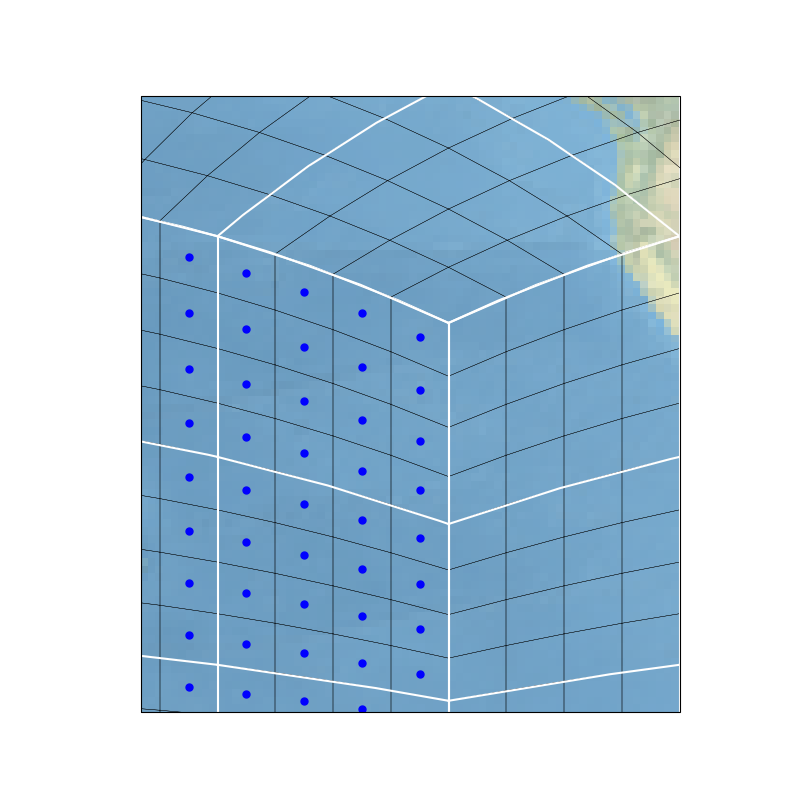
\includegraphics[width=0.8\linewidth]{duoscalar1}
		\caption{A-grid values (blue circles).\label{cs-duoscalar-1}}
	\end{subfigure}
	\begin{subfigure}{0.45\textwidth}
		\centering
		\includegraphics[width=0.8\linewidth]{duoscalar2}
		\caption{Kinked A-grid values (red and green circles)\label{cs-duoscalar-2}}
	\end{subfigure}

	\begin{subfigure}{0.45\textwidth}
		\centering
		\includegraphics[width=0.8\linewidth]{duoscalar3}
		\caption{A duo-grid values (blue squares)\label{cs-duoscalar-3}}
	\end{subfigure}
	\begin{subfigure}{0.45\textwidth}
	\centering
	\includegraphics[width=0.8\linewidth]{duoscalar4}
	\caption{Interpolation lines (dashed blue lines)\label{cs-duoscalar-4}}
    \end{subfigure}
 	\caption{Illustration of the A duo-grid interpolation for a scalar field. \label{cs-duoscalar}}
\end{figure}

To illustrate this process in Panel 1, we depict the values of $q_{ijp}$ in Figure \ref{cs-duoscalar}. 
The blue circles represent the values in Panel 1 (Figure \ref{cs-duoscalar-1}), while the red and green circles 
represent the so called \textbf{kinked} values in the other panels (Figure \ref{cs-duoscalar-2}). 
Assuming a halo size of 3, we also indicate the target values at the ghost cell 
positions using blue squares (Figure \ref{cs-duoscalar-3}). 
It is worth noting that the dashed blue lines in Figure \ref{cs-duoscalar-4} 
illustrate how the ghost cell points lie on geodesics containing grid positions from adjacent panels.
With the exception of the blue squares that lie on a cube corner (Figure \ref{cs-duoscalar-4}),
all the ghost cell values can be obtained using 1D Lagrange interpolation, 
utilizing the surrounding red/green circles on the geodesic. 
This interpolation procedure can be performed for all panels. 
Subsequently, the blue squares located on a cube corner can be interpolated using the 
green and red points by connecting these points using geodesics and further extending the blue lines from Figure \ref{cs-duoscalar-4}.

There are two ways of computing the Lagrange polynomials.
The first one is based on the geodesic distances of the duo-grid line points.
This approach was explored in \citet{chen:2021} and \citet{mouallem:2023}, and we are going to consider it here, calling it \textbf{dg1}.
The second one is to use cube-based distances, where all duo-grid and kinked points are remapped to the plane using the inverse of the cube mapping. 
This approach has the advantage of having uniformly spaced data (the remapped kinked values) used in the duo-grid points interpolation.
This approach is called \textbf{dg2}.
\begin{figure}[!htb]
	\centering
	\includegraphics[width=0.8\linewidth]{h_tc-4_t0_alpha45_C192_g2.s_dg2_adv1_hord8_tf12}
	\caption{Scalar field from Equation \eqref{duo-tc1}.\label{cs-duo-tc1}}
\end{figure}

We are going to show a numerical example of this interpolation process using a halo region of size 3 and cubic polynomials.
We shall consider the following trigonometric function
from test case 2 in \citet{will:1992} in our tests:
\begin{equation}
\label{duo-tc1}
q(\lambda, \phi) = h_0 - \frac{1}{g}\bigg(R\Omega u_0 + \frac{u_0^2}{2}\bigg)
\bigg( -\cos(\lambda)\cos(\phi)\sin(\alpha) + \sin(\phi)\cos(\alpha) \bigg)^2,
\end{equation}
where $h_0 = 3\times 10^3 $,
$\alpha=\frac{\pi}{4}$, $u_0 = \frac{2\pi R}{12 \text{days}}$,  $g=9.8$ is the gravity and $\Omega=7.2921 \times 10^{-5}$ is the Earth angular rotation speed.
In Figure \ref{cs-duo-tc1} we depict the graph of this field.

We compute the maximum errors for values of $N$ of the form $N=48\times2^k$, where $k$ ranges from 0 to 4. 
We consider g0.s and g0.c, each one with dg1 and dg2, whose errors are depicted in Figure \ref{cs-duoscalar-tc1-g0}.
Additionally, we analyze g2.s and g2.c, each one with dg1 and dg2, and their errors are illustrated in Figure \ref{cs-duoscalar-tc1-g2}.

From the dashed lines in Figure \ref{cs-tc1-error}, we observe that both dg1 and dg2 achieve fourth-order accuracy when the midpoints use the cube formulation, 
with dg2 being much more accurate than dg1.
However, when spherical midpoints are employed, we observe a reduction in accuracy by two orders, as indicated by the solid lines.
Both dg1 and dg2 are very similar in this case.
This discrepancy arises due to a second-order mismatch between cube and spherical midpoints, as discussed in Section \ref{duogrid-points}.
Finally, we observe that the equi-edge grid (g0) yields slightly better results than the equiangular grid (g2) for the cube midpoints formulation.
\begin{figure}[!htb]
	\centering
	\begin{subfigure}{0.45\textwidth}
		\centering
		\includegraphics[width=1\linewidth]{g0_duo_error_tc-2_ha}
		\caption{Error for equi-edge (g0).\label{cs-duoscalar-tc1-g0}}
	\end{subfigure}
	\begin{subfigure}{0.45\textwidth}
		\centering
		\includegraphics[width=1\linewidth]{g2_duo_error_tc-2_ha}
		\caption{Error for g2.\label{cs-duoscalar-tc1-g2}}
	\end{subfigure}
	\caption{Error for the duo-grid interpolation of the scalar field of \eqref{duo-tc1} for the equi-edge grid (g0, left) and the equiangular grid (g2, right).
Dashed lines use the cube midpoint formulation, while solid lines use the spherical midpoint formulation.
Green lines represent dg1, and red lines represent dg2.\label{cs-tc1-error}}
\end{figure}


\subsection{Ghost cells wind interpolation}
\label{cs-wind-interp}
Let us consider the following problem: Assume that we are given a tangent vector field of the sphere, denoted as 
$\boldsymbol{u}:\mathbb{S}^2_R \to \mathbb{R}^3$. We also have its normalized covariant normal components at the edge points, 
namely $u_{i+\frac{1}{2},j,p}$ for $i=0, \ldots, N$ and $j=1, \ldots, N$, as well as
$v_{i,j+\frac{1}{2},p}$ for $i=1, \ldots, N$ and $j=0, \ldots, N$. This grid function is called C-grid wind following \citet{arakawa:1977} (Figure \ref{cs-duovec-1}).

Our objective is to obtain the values 
\begin{align*}
	u_{i+\frac{1}{2},j,p} \quad \text{ for} \quad &i=-1, \ldots, N+1, \quad &j=-\nu+1, \ldots, 0, \quad &j=N, \ldots, N+\nu,\\
	v_{i,j+\frac{1}{2},p} \quad \text{ for} \quad &j=0, \ldots, N, \quad &i=-\nu+1, \ldots, 0,\quad &i=N, \ldots, N+\nu.
\end{align*}
This problem arises when we apply the dimension splitting method on each panel of the cubed-sphere.
\begin{figure}[!htb]
	\centering
	\begin{subfigure}{0.45\textwidth}
		\centering
		\includegraphics[width=0.8\linewidth]{duowind1}
		\caption{C-grid wind values (blue and red squares).\label{cs-duovec-1}}
	\end{subfigure}
	\begin{subfigure}{0.45\textwidth}
		\centering
		\includegraphics[width=0.8\linewidth]{duowind2}
		\caption{A-grid wind (black circles)\label{cs-duovec-2}}
	\end{subfigure}
	
	\begin{subfigure}{0.45\textwidth}
		\centering
		\includegraphics[width=0.8\linewidth]{duowind3}
		\caption{A-duo-grid points (green circles)\label{cs-duovec-3}}
	\end{subfigure}
	\begin{subfigure}{0.45\textwidth}
		\centering
		\includegraphics[width=0.8\linewidth]{duowind4}
		\caption{C-duo-grid  wind values (green circles) \label{cs-duovec-4}}
	\end{subfigure}
	\caption{Illustration of the C duo-grid interpolation for a C-grid wind. \label{cs-duovec}}
\end{figure}

\begin{figure}[!htb]
	\centering
	\begin{subfigure}{0.45\textwidth}
		\centering
		\includegraphics[width=1\linewidth]{g0_duo_error_tc-2_uc}
		\caption{Error for equi-edge grid (g0).\label{cs-duoscalar-tc2-g0}}
	\end{subfigure}
	\begin{subfigure}{0.45\textwidth}
		\centering
		\includegraphics[width=1\linewidth]{g2_duo_error_tc-2_uc}
		\caption{Error for equiangular grid (g2).\label{cs-duoscalar-tc2-g2}}
	\end{subfigure}
	\caption{As Figure \ref{cs-tc1-error} but using the C-grid wind given by Equation \eqref{duo-wind1}.\label{cs-tc2-error}}
\end{figure}

This problem can be solved by using the duo-grid interpolation process described earlier for a scalar field.
To apply that interpolation process, we first need to interpolate the values of $u$ and $v$ from the
edges to the center points required for the ghost cells interpolation (Figure \ref{cs-duovec-2}).
Specifically, we need the values:
\begin{align*}
	u_{1+k,j,p}, v_{1+k,j,p} \quad \text{ for} \quad &j=1, \ldots, N, \quad k=0, \ldots, \nu,\\
	u_{N-k,j,p}, v_{N-k,j,p} \quad \text{ for} \quad &j=1, \ldots, N, \quad k=0, \ldots, \nu,\\
	u_{i,1+k,p}, v_{i,1+k,p} \quad \text{ for} \quad &i=1, \ldots, N, \quad k=0, \ldots, \nu,\\
	u_{i,N-k,p}, v_{i,N-k,p} \quad \text{ for} \quad &i=1, \ldots, N, \quad k=0, \ldots, \nu.\\
\end{align*}
We apply a simple linear interpolation to remap $u$ and $v$ to the center points (Figure \ref{cs-duovec}).
Then we obtain two A-grid scalar fields, and we may proceed as before to fill the ghost cell values.
However, we are going to use one extra layer of A-grid values since they will be needed for re-interpolation to the edge points.
For instance, for 3 layers of ghost cells, we need 4 layers of A duo-grid values to fill the C-grid wind at the duo-grid edge points, as shown in Figure \ref{cs-duovec-2}.
Once these interpolated values are computed, we convert the covariant values $u_{ijp}, v_{ijp}$
to their latitude-longitude components $(u_{\lambda})_{ijp}, (v_{\phi})_{ijp}$ using Equations \eqref{norm-contravariant-to-covariant} and
\eqref{ll-to-normcontravariant}.
This conversion avoids any coordinate system discontinuity, as this interpolation is performed only close to the cube edges and far from the poles.
Then, we can use the ghost cell centers interpolation procedure described before for the latitude-longitude components
to recover the wind at the ghost cell centers using any polynomial degree (Figures \ref{cs-duovec-3}).
Finally, we can use the values at the ghost cell centers to obtain the values at the ghost cell edges
by employing a linear interpolation once again (Figures \ref{cs-duovec-4}).
Subsequently, the covariant components can be obtained by using Equations \eqref{ll-to-normcontravariant} and \eqref{norm-contravariant-to-covariant}.

We will consider the following rotated zonal field, as a numerical test, based on \citet{will:1992}:
\begin{align}
	\label{duo-wind1}
	\begin{cases}
		u_\lambda(\lambda,\phi,t) = u_0(\cos(\phi)\cos(\alpha) + \sin(\phi)\cos(\lambda)\sin(\alpha)),\\
		v_\phi(\lambda,\phi,t) = -u_0\sin(\lambda)\sin(\alpha).
	\end{cases}
\end{align}
Here,  $u_0 = \frac{2\pi R}{12 \text{days}}$ and $\alpha= \frac{\pi}{4}$. We will adopt the same grids and schemes as in Section \ref{cs-interp}.
Next, we will compute the relative errors of the covariant components at the edge midpoints.
The errors are presented in Figure \ref{cs-tc2-error}, along with the convergence rate for different schemes employed in the ghost cell center interpolation.
We emphasize that, since we utilize a linear interpolation to retrieve the A-grid wind components from the edge midpoints, as well as in the interpolation
from the center duo-grid points to edge duo-grid points, the maximum attainable scheme order is 2.
Indeed, from Figure \ref{cs-tc2-error}, we observe that when employing a cubic polynomials in the duo-grid interpolation step, the final order achieved is 2.
We can also observe again that the spherical midpoints yield larger errors than the cube midpoints formulation.
Additionally, dg2 yields smaller errors, and overall, equi-edge (g0) performs slightly better than the equiangular (g2) grid.


\newpage
\subsection{Edges reconstruction}
\label{cs-recon}
Let us consider the following problem: given the values $q_{ijp}$ we wish to find 
approximations of the function $q$ at the edge points denoted by
\begin{align*}
	q^{L,x}_{ijp}  \approx q_{{i-\frac{1}{2}},j,p},\quad
	q^{R,x}_{ijp}  \approx q_{{i+\frac{1}{2}},j,p},\quad
	q^{L,y}_{ijp}  \approx q_{i,{j-\frac{1}{2}},p},\quad
	q^{R,y}_{ijp}  \approx q_{i,{j+\frac{1}{2}},p}.
\end{align*}

We can estimate the desired values by using the one-dimensional reconstruction schemes 
described in Section \ref{chp-adv1d-sec-recon},
performing PPM reconstruction independently in the $x$ and $y$ directions. 
It is worth noting that all the schemes discussed in those sections are 
expected to be second-order accurate due to the centroid point approximation.

There are  some differences in the computation of the stencil near the cube edges.
Unlike in the previous chapters, where periodic boundary conditions were assumed, 
the boundary conditions in this context are related to the adjacent panels. 
One way to address this issue is to use the duo-grid as discussed  in Section \ref{cs-interp} to compute the stencils. 
We are going to consider the dg2 method, since it yields better results overall.

Another approach, employed in \citet{sadourny:1972}, involves ignoring the
discontinuity of the coordinate system and simply using the values of the cells 
in the adjacent panels as the ghost cell values. 
Additionally, an alternative method that avoids the use of ghost cells was developed by
\citet{putman:2007}, which entails extrapolation at the cells surrounding the cube edge.
We will refer to this scheme as \textbf{kinked} method.
This scheme uses the following extrapolations:
\begin{align*}
	q^{L,x}_{1,j,p} &= \frac{1}{2}\bigg(3Q_{1,j,p} - Q_{2,j,p}\bigg),\\
	q^{R,x}_{N,j,p} &= \frac{1}{2}\bigg(3Q_{N,j,p} - Q_{N-1,j,p}\bigg),
\end{align*}
at the points that are located on the cube edges. The other edge values are estimated as:
\begin{align*}
	q^{R,x}_{1,j,p} &= \frac{1}{14}\bigg(3Q_{1,j,p} + 11Q_{2,j,p} - 2(Q_{3,j,p} - Q_{1,j,p})\bigg),\\
	q^{L,x}_{2,j,p} &= q^{R,x}_{1,j,p},\\
	q^{L,x}_{N,j,p} &= \frac{1}{14}\bigg(3Q_{N,j,p} + 11Q_{N-1,j,p} - 2(Q_{N-2,j,p} - Q_{N,j,p})\bigg),\\
	q^{R,x}_{N-1,j,p} &= q^{L,x}_{N,j,p},\\
\end{align*}
in the $x$ direction. Similar formulas are used in the $y$ direction.
We are going to use the trigonometric function (Equation \eqref{duo-tc1})
as before on the unit sphere to compare the schemes kinked and dg2. The scheme dg2 uses cubic polynomials.
We introduce the relative errors:
\begin{align*}
	e_{{i-\frac{1}{2}},j,p} &= (|q_{{i-\frac{1}{2}},j,p} - q^{L,x}_{ijp}|)/|q_{{i-\frac{1}{2}},j,p}|,\\
	e_{{i+\frac{1}{2}},j,p} &= (|q_{{i+\frac{1}{2}},j,p} - q^{R,x}_{ijp}|)/|q_{{i+\frac{1}{2}},j,p}|,\\
	e_{i,{j-\frac{1}{2}},p} &= (|q_{i,{j-\frac{1}{2}},p} - q^{L,y}_{ijp}|)/|q_{i,{j-\frac{1}{2}},p}|,\\
	e_{i,{j+\frac{1}{2}},p} &= (|q_{i,{j+\frac{1}{2}},p} - q^{R,y}_{ijp}|)/|q_{i,{j+\frac{1}{2}},p}|,\\
	e_{ijp} &= \max\{e_{{i-\frac{1}{2}},j,p}, e_{{i+\frac{1}{2}},j,p} , e_{i,{j-\frac{1}{2}},p}, e_{i,{j+\frac{1}{2}},p} \},\\
	E &= \max \{e_{ijp}\}.
\end{align*}
We are going to compute $E$ for different values of $N$ as in the numerical experiments of Section \ref{cs-interp}.
We consider the kinked scheme for the grids g0.s and g2.s, and the dg2 scheme for the grids g0.s, g0.c, g2.s, and g2.c.
The reconstruction scheme employed is the limited PPM (hord8). We depict the errors in Figure \ref{cs-recon-error}.
We can observe that the error for the equi-edge grid (g0) is only slightly better than the error for the equiangular grid (g2).
Also, the errors for the cube midpoint formulation and the spherical midpoint formulation are essentially the same when using dg2.
\begin{figure}[!htb]
	\centering
	\begin{subfigure}{0.45\textwidth}
		\centering
		\includegraphics[width=1\linewidth]{hord8_recon_g0.c}
		\caption{Error for equi-edge (g0).\label{cs-recon-g0}}
	\end{subfigure}
	\begin{subfigure}{0.45\textwidth}
		\centering
		\includegraphics[width=1\linewidth]{hord8_recon_g2.c}
		\caption{Error for g2.\label{cs-recon-g2}}
	\end{subfigure}
	\caption{Relative error for the PPM reconstruction using scalar field from Equation \eqref{duo-tc1}.
	Equi-edge (g0) grid results are on the left, and equiangular grid (g2) results are on the right.
	Green lines represent g2.s with the kinked method;
	red lines represent g2.s with dg2;
	blue lines represent g2.c with dg2.
	The reconstruction scheme is the limited PPM (hord8).\label{cs-recon-error}}
\end{figure}

From Figure \ref{cs-recon-error}, we see that the dg2 method leads to second-order accuracy, while the kinked method leads to first-order accuracy.
Since the kinked and dg2 affect the PPM reconstruction only near to the cube edges, we expect that the error of the kinked  method is larger only at the corners, leading to grid imprinting.
Indeed, in Figure \ref{recon-errors-g0}, we depict the logarithm of the error (on base 10 for plotting purposes) for the equi-edge (g0) grids.
It becomes clear from Figure \ref{recon-errors-g0-s} that the kinked method leads to grid imprinting,
while Figures \ref{recon-errors-g0-s-dg} and \ref{recon-errors-g0-c-dg} show that dg2 introduces less grid imprinting.
Figure \ref{recon-errors-g2} shows similar results to Figure \ref{recon-errors-g0}, but considering the equiangular grid instead, from which we can draw similar conclusions.
In general, dg2 is not sensitive to changing midpoints formulation.
Additionally, the kinked method exhibits less grid imprinting in the equi-edge grid (Figure \ref{recon-errors-g0-s}) than in the equiangular grid (Figure \ref{recon-errors-g2-s}).

\newpage
\begin{figure}[!ht]
	\centering
	\begin{subfigure}{0.9\textwidth}
		\centering
		\includegraphics[width=1\linewidth]{recon_g0_192.s.kinked.hord8}
		\caption{g0.s with kinked. \label{recon-errors-g0-s}}
	\end{subfigure}
	
	\begin{subfigure}{0.9\textwidth}
		\centering
		\includegraphics[width=1\linewidth]{recon_g0_192.s.dg2.hord8}
		\caption{g0.s with dg2.\label{recon-errors-g0-s-dg}}
	\end{subfigure}
	
	\begin{subfigure}{0.9\textwidth}
		\centering
		\includegraphics[width=1\linewidth]{recon_g0_192.c.dg2.hord8}
		\caption{g0.c with dg2.\label{recon-errors-g0-c-dg}}
	\end{subfigure}
	\caption{The logarithm in base 10 of the errors of the edge grid points reconstruction from the A-grid field
		given by Equation \eqref{duo-tc1}, using the equi-edge grid (g0) with $N=192$. \label{recon-errors-g0}}
\end{figure}

\newpage
\begin{figure}[!ht]
	\centering
	\begin{subfigure}{0.9\textwidth}
		\centering
		\includegraphics[width=1\linewidth]{recon_g2_192.s.kinked.hord8}
		\caption{g0.s with kinked. \label{recon-errors-g2-s}}
	\end{subfigure}
	
	\begin{subfigure}{0.9\textwidth}
		\centering
		\includegraphics[width=1\linewidth]{recon_g2_192.s.dg2.hord8}
		\caption{g0.s with dg2.\label{recon-errors-g2-s-dg}}
	\end{subfigure}
	
	\begin{subfigure}{0.9\textwidth}
		\centering
		\includegraphics[width=1\linewidth]{recon_g2_192.c.dg2.hord8}
		\caption{g0.c with dg2.\label{recon-errors-g2-c-dg}}
	\end{subfigure}
	\caption{As Figure \ref{recon-errors-g0} but using the equiangular grid (g2). \label{recon-errors-g2}}
\end{figure}


\section{Concluding remarks}
\label{cs-conc}
In this Chapter, we reviewed cubed-sphere mappings with a special focus on the equiangular and equi-edge mappings,
which leads to a more uniform cubed-sphere grid, with the equiangular grid being the most uniform.
The corner points are generated using the equiangular and equi-edge mappings;
however, the center and edge points may be generated using a cubed-sphere mapping or using midpoints based on spherical midpoints of the corner points
(Section \ref{cs-geo}).


We observed that the equiangular cubed-sphere ghost cells, obtained by extending the gridlines, have a nice property:
their edge and center ghost points are located on a common geodesic that contains the edge and center points of the adjacent panels. 
This property allows us to use 1D Lagrange interpolation to obtain the values of scalar and vector fields in the ghost cells.
The equi-edge grid does not have this property, but we may mirror some points to make its ghost cells have the same property as in the equiangular grid.
In fact, we demonstrated the accuracy of this interpolation on the duo-grid method through numerical examples in Sections \ref{cs-interp} and \ref{cs-wind-interp}.
We explored two ways of computing the Lagrange polynomials: one based on the geodesic distances and the other based on local coordinate distances.
Overall, the method based on local coordinate distances showed that it introduces smaller errors,
especially when using the cube midpoints formulation instead of the spherical midpoints formulation.

Afterward, in Section \ref{cs-recon}, we investigated different methods for computing stencils near the cube edges.
We considered the scheme based on 1D Lagrange interpolation and a scheme based on extrapolations from \citet{putman:2007}, which is currently implemented in FV3.
Through numerical examples, we demonstrated that the reconstruction at cell edges using the limited PPM (hord8) scheme generates grid imprinting near
the cubed edges when using extrapolations.
The grid imprinting is greatly reduced when we apply the duo-grid Lagrange interpolation, which shows that this scheme is much better for filling the ghost cells of the cube panels.

One major conclusion of this Chapter is that the cube and spherical midpoints formulation have a second-order difference.
This impacts severely on the duo-grid interpolation step, where we attain the expected orders of interpolation only for the cube midpoints formulation.
However, in the reconstruction from center to edge midpoints, both formulations have essentially the same errors.
Hence, we expect that both midpoint formulations should lead to the very similar results.



\chapter{Cubed-sphere finite-volume methods}
\label{chp-cs-fv}
Now that we have described in Chapter \ref{chp-cs-grids} how we can obtain the ghost cell values of each panel on the cubed-sphere using Lagrange interpolation, we are ready to apply the dimension-splitting methods presented in Chapter \ref{chp-2d-fv} to solve the advection equation on the cubed-sphere.
One significant difference is that we have the metric term, which is not present in the plane simulations.
Additionally, when employing ghost cell layers using the duo-grid, the flux at the cube edges is computed twice, 
requiring the averaging of fluxes at the edges to ensure a unique value in order to achieve mass conservation.


This Chapter is organized as follows: Section \ref{chp-cs-adv} introduces the advection equation on the cubed-sphere.
Section \ref{chp-cs-fvcs} presents its finite-volume discretization with a focus on the extension of dimension splitting (Section \ref{sec-csdsplit}) 
as presented in Section \ref{sec-dsplit}.
Numerical experiments are presented in Section \ref{chp-cs-numexpadv}, where we use dimension splitting to assess its
accuracy in computing the divergence of a given vector field to check its numerical consistency, as well as to solve the advection equation.
In particular, we explore different treatments for the cube edges. Section \ref{chp-cs-conc} presents the final thoughts.

\section{Cubed-sphere advection equation in integral form}
\label{chp-cs-adv}
Given a tangent velocity field $\boldsymbol{u}$ on the sphere, we denote its
contravariant components by $\mathfrak{u}$ and $\mathfrak{v}$.
We shall use all the notations introduced in Section \ref{cs-notation}.
The advection equation on panel the $p$ of the cubed-sphere with initial condition $q_0$ is given by:
\begin{equation}
	\begin{cases}
		\label{eq1-adv-cs}
		\bigg[{\partial}_t{q}+
		\frac{1}{\sqrt{\mathfrak{g}}}\bigg(
		{\partial}_x{(\mathfrak{u} q \sqrt{\mathfrak{g}})}+
		{\partial}_y{(\mathfrak{v} q \sqrt{\mathfrak{g}})}
		\bigg)\bigg](x,y,p,t)
		= 0,\\
		q(x,y,p,0) = q_0(x,y,p),
	\end{cases}
\end{equation}
$\forall (x,y) \in \Omega := [-\alpha,\alpha]^2$, $t\in[0,T]$.
We denote by $\nabla \cdot (q\boldsymbol{u})$ the divergence operator:
\begin{equation}
	\label{advcs:eqdiv}
	\nabla \cdot (q\boldsymbol{u})(x, y, p, t) =  \frac{1}{\sqrt{\mathfrak{g}}}
	[{\partial_x (\mathfrak{u}q\sqrt{\mathfrak{g}})} + {\partial_y (\mathfrak{v}q\sqrt{\mathfrak{g}})}](x, y, p, t).
\end{equation}
We recall that we say the $\boldsymbol{u}$ is \textbf{non-divergent} if $\nabla \cdot \boldsymbol{u}=0$.
We define the $\mathcal{CS}_N$ grid function $\delta^n$ as
the exact divergence of $q\boldsymbol{u}$ at the cell centers, namely
\begin{equation}
	\label{cs-discrete-div}
	\delta^n_{ijp} = \nabla \cdot (\boldsymbol{u}q)(x_i,y_j,p,t^n).
\end{equation}
In this Chapter, it shall be useful to define the average value of $q\sqrt{\mathfrak{g}}$ on the 2D coordinates as:
\begin{equation}
\label{cs-q-av}
\overline{(\sqrt{\mathfrak{g}}q)}_{ijp}(t) = \frac{1}{\Delta x \Delta y}
\int_{x_{i-\frac{1}{2}}}^{x_{i+\frac{1}{2}}}
\int_{y_{j-\frac{1}{2}}}^{y_{j+\frac{1}{2}}}  q(x,y,p,t) {\sqrt{\mathfrak{g}}(x,y)}\,dx \,dy.
\end{equation}
This average value simplifies the deduction of finite-volume method on the cubed-sphere instead of using the spherical average values (Equation \eqref{qav-sphere}).
Since the metric term does not depend on $t$, we may rewrite Equation \eqref{eq1-adv-cs} as
\begin{equation}
	\label{eq2-adv-cs}
	\bigg[{\partial}_t{(q \sqrt{\mathfrak{g}})}+
	{\partial}_x{(\mathfrak{u}q \sqrt{\mathfrak{g}})}+
	{\partial}_y{(\mathfrak{v}q \sqrt{\mathfrak{g}})}
	\bigg](x,y,p,t)
	= 0.
\end{equation}
Therefore, as in Problem \eqref{chp-adv2d-sec2-prob1}, the integral form of Equation \eqref{eq1-adv-cs}
is stated in Problem \eqref{chp5-prob1}.
\begin{prob}
	\label{chp5-prob1}
	Given an initial condition ${q}_0$ and
	a velocity on the sphere $\boldsymbol{u}$, with contravariant components $(\mathfrak{u},\mathfrak{v})$ on the cubed-sphere coordinate system,
	we would like to find a weak solution ${q}$
	of the cubed-sphere advection equation in its integral form:
	\begin{align*}
		\int_{x_1}^{x_2} \int_{y_1}^{y_2}
		{(q\sqrt{\mathfrak{g}})}(x, y, p, t) \,dx \,dy = &\int_{x_1}^{x_2} \int_{y_1}^{y_2}
		{(q\sqrt{\mathfrak{g}})}(x, y, p, t) \,dx \,dy \\ \nonumber
		&-\int_{t_1}^{t_2} \int_{y_1}^{y_2} \bigg({(\mathfrak{u}q\sqrt{\mathfrak{g}})}(x_2, y, t)
		-{(\mathfrak{u}q\sqrt{\mathfrak{g}})}(x_1, y, t) \bigg) \,dy \,dt\\ \nonumber
		&-\int_{t_1}^{t_2} \int_{x_1}^{x_2} \bigg({(\mathfrak{v}q\sqrt{\mathfrak{g}})}(x, y_2, t)
		-{(\mathfrak{v}q\sqrt{\mathfrak{g}})}(x, y_1, t) \bigg) \,dx \,dt.
	\end{align*}
	$\forall [x_1, x_2]\times [y_1, y_2] \times[t_1, t_2] \subset \Omega \times[0,T]$, and
	$q(x,y,p,0)=q_0(x,y,p)$.
\end{prob}
Similarly to Section \ref{chp-adv2d-sec1}, Equation \eqref{eq1-adv-cs} and Problem \eqref{chp5-prob1} are equivalent
when ${q}, \boldsymbol{u} \in \mathcal{C}^1(\mathbb{S}^2_R)$.
For Problem \ref{chp5-prob1}, the total mass in $\mathbb{S}^2_R$ is defined by: 
\begin{equation}
	{M}_{\mathbb{S}^2_R}(t) = \sum_{p=1}^6 \int_{\Omega} {(q\sqrt{\mathfrak{g}})}(x,y,p,t) \,dx \,dy , \quad \forall t \in [0,T],
\end{equation}
and is conserved within time: 
\begin{equation}
	{M}_{\mathbb{S}^2_R}(t) = {M}_{\mathbb{S}^2_R}(0), \quad \forall t \in [0,T].
\end{equation}
We define a discretized version of Problem \eqref{chp5-prob1} as Problem \eqref{chp5-prob2}.
\begin{prob}
	\label{chp5-prob2}
	Assume the framework of Problem \ref{chp5-prob1}
	and consider a $(\Delta x, \Delta y, \Delta t, \lambda)$-discretization of $\Omega\times [0,T]$, with $\Delta x= \Delta y$.
	Since we are in the framework of Problem \ref{chp5-prob1}, it follows that:
	\begin{align*}
		\overline{(\sqrt{\mathfrak{g}}q)}_{ijp}(t_{n+1})  = \overline{(\sqrt{\mathfrak{g}}q)}_{ijp}(t_{n})
		&- { \lambda}
		\delta _x \bigg( \frac{1}{\Delta t \Delta y}
		\int_{t^n}^{t^{n+1}} \int_{y_{j-\frac{1}{2}}}^{y_{j+\frac{1}{2}}} 
		{(\mathfrak{u}q\sqrt{\mathfrak{g}})}(x_{i}, y, p, t)
		\,dy \,dt \bigg) \\ \nonumber
		&- {\lambda}
		\delta _y \bigg( \frac{1}{\Delta t \Delta x}
		\int_{t^n}^{t^{n+1}} \int_{x_{i-\frac{1}{2}}}^{x_{i+\frac{1}{2}}} 
		{(\mathfrak{v}q\sqrt{\mathfrak{g}})}(x, y_{j}, p, t)
		\,dx \,dt \bigg),
	\end{align*}
	where
	\begin{equation}
		\overline{(\sqrt{\mathfrak{g}}q)}_{ijp}(t) = \frac{1}{\Delta x \Delta y}
		\int_{x_{i-\frac{1}{2}}}^{x_{i+\frac{1}{2}}} 
		\int_{y_{j-\frac{1}{2}}}^{y_{j+\frac{1}{2}}} {(q\sqrt{\mathfrak{g}})}(x,y,p,t) \,dx \,dy.
	\end{equation}
	Our problem now consists of finding the values ${Q}_{ijp}(t_{n})$, 
	$\forall i = 1, \ldots, N$, $\forall j = 1, \ldots, M$, $\forall n = 0, \ldots, N_T-1$,
	given the initial values ${(\sqrt{\mathfrak{g}}q)}_{ijp}(0)$, $\forall i = 1, \ldots N$, $\forall j = 1, \ldots, M$.
	In other words, we aim to find the average values of ${(\sqrt{\mathfrak{g}}q)}_{ijp}$ in each control volume $\Omega_{ijp}$ at the specified time instances.
\end{prob}
It is important to note that no approximations have been made in Problems \eqref{chp5-prob1} and \eqref{chp5-prob2}. 
%In practice, the term $\frac{\Delta x  \Delta y}{|\Omega_{ijp}|}$ is estimated using the second-order
%formula obtained by applying the midpoint rule in Equation \eqref{chp4-area}:
%\begin{equation}
%	\frac{\Delta x  \Delta y}{|\Omega_{ijp}|}= \frac{1}{\sqrt{\mathfrak{g}}_{ijp}} + O(\Delta x^2).
%\end{equation}
\section{Finite-volume on the cubed-sphere approach}
\label{chp-cs-fvcs}
We are ready to introduce the finite-volume scheme on the cubed-sphere (CS-FV).
A CS-FV scheme problem as follows in Problem \ref{chp5-prob3}.
Before that, we consider the following approximation, which follows from the midpoint rule (Theorem \ref{prop-bound-midpoint2d}):
\begin{equation}
	\label{midpoint-approx}
	\overline{(\sqrt{\mathfrak{g}}q)}_{ijp}(t)  = \sqrt{\mathfrak{g}_{ij}} {q}_{ijp}(t) +\mathcal{O}(\Delta x^2).
\end{equation}
We use this approximation in Problem{chp5-prob2} and we obtain the following CS-FV scheme:
\begin{prob}[CS-FV scheme]
	\label{chp5-prob3}
	Assume the framework defined in Problem \ref{chp5-prob2}.
	The finite-volume approach of Problem \ref{chp5-prob1}
	consists of a finding a scheme of the form:
	\begin{align}
		\label{chp5-csfv}
		{q}_{ijp}^{n+1} =  {q}_{ijp}^{n} - \frac{\lambda}{\sqrt{\mathfrak{g}}_{ij}} \delta_i {F}_{ijp}^{n}
		-  \frac{\lambda}{\sqrt{\mathfrak{g}}_{ij}}  \delta_j {G}_{ijp}^{n},
		\\ \nonumber \quad \forall i = 1, \ldots, N, \quad \forall j = 1, \ldots, M, \quad p =1, \ldots, 6,
		\quad \forall n = 0, \ldots, N_T-1,
	\end{align}
	where $ \delta_i F_{ijp}^n =
	{F}_{i+\frac{1}{2},j,p}^{n} 
	- {F}_{i-\frac{1}{2},j,p}^{n}$,
	$ \delta_j G_{ijp}^n =
	{G}_{i,j+\frac{1}{2},p}^{n} 
	- {G}_{i,j-\frac{1}{2},p}^{n}$ 
	and ${q}^{n}\in \mathcal{CS}_N$ is intended to be an approximation
	of ${q}(t_{n})\in \mathcal{CS}_N$ in some sense. We define
	${q}_{ijp}^{0} = {q}^0_{ijp}$.
	
	The term ${F}_{i+\frac{1}{2}, j, p}^{n}$ is known as numerical flux in the 
	$x$ direction and it approximates
	$\frac{1}{\Delta t \Delta y }\int_{t_n}^{t_{n+1}} 
	\int_{y_{j-\frac{1}{2}}}^{y_{j+\frac{1}{2}}} 
	(\mathfrak{u}q\sqrt{\mathfrak{g}})(x_{i+\frac{1}{2}}, y, p, t) \,dy \,dt $,
	$\forall i = 0, 1, \ldots, N$, and 
	${G}_{i, j+\frac{1}{2}, p}^{n}$ is known as numerical flux in the 
	$y$ direction and it approximates
	$\frac{1}{\Delta t\Delta x}\int_{t_n}^{t_{n+1}}  
	\int_{x_{i-\frac{1}{2}}}^{x_{i+\frac{1}{2}}}
	(\mathfrak{v}q\sqrt{\mathfrak{g}})(x, y_{j+\frac{1}{2}}, p, t) \,dx \,dt $,
	$\forall j = 0, 1, \ldots, M$,
	or, in other words, they estimate the time-averaged
	fluxes at the control volume $\Omega_{ijp}$ boundaries.
\end{prob}
\begin{remark}
	For Problem \ref{chp5-prob3}, we define the CFL number in the $x$ and $y$ direction
	by $\max \{{|\mathfrak{u}_{i+\frac{1}{2},j,p}^n}|\}\frac{\Delta t}{\Delta x}$ and 
	$\max \{ {|\mathfrak{v}_{i,j+\frac{1}{2},p}^n}|\}\frac{\Delta t}{\Delta y}$, respectively.
	The CFL number is maximum between these numbers and we say that the CFL condition is
	satisfied if the CFL number is less than one. 
\end{remark}
As we mentioned in Problem \ref{chp5-prob3}, the initial condition may be assumed as $q_{ijp}^0$ or $Q_{ijp}(0)$.
We are going to assume  $q_{ijp}^0$ as initial data to avoid the computation of integrals.
Furthermore, the errors will be calculated using the values $q_{ijp}^n$ instead of $Q_{ijp}(t_n)$.
As in Section \ref{sec:fv-2d} this approximation leads to a second-order error.


\section{Dimension splitting}
\label{sec-csdsplit}
In this Section, we will utilize the dimension splitting method described in Section \ref{sec-dsplit} to obtain a CS-FV scheme.
To facilitate notation, we shall omit the index $p$ whenever it may appear in this Section, as what is described here does not depend on $p$.
Also, the ghost cell values are assumed to be filled using the duo-grid interpolation.
\subsection{PPM and the metric term}
\label{sec-metricppm}
Recall that the dimension splitting technique requires the numerical solution of advection in the $x$ and $y$ directions for separability.
For instance, in the case of the advection equation on the cubed-sphere (Equation \eqref{eq2-adv-cs}), we need to solve the following equations in the $x$ direction:
\begin{equation}
	\label{1d-avd-eq}
		[{\partial_t (\sqrt{\mathfrak{g}} {q^x})} + {\partial_x (\mathfrak{u}\sqrt{\mathfrak{g}}{q^x}})](x, y_j, p, t),
\end{equation}
for $j=-\nu+1, \ldots, N+\nu$, at certain time levels $t^n$, $n=1, \ldots, N_T$ (Section \ref{lit-trotter-sp}).
We are particularly interested in approximating $q^{x,n+1}_{ij}$ for $i=1, \ldots, N$, which represents the values of $q^x$ at the cell centroids.
This involves providing an approximation of the solution to Equation \eqref{eq2-adv-cs}, 
denoted as $q^n_{ij}$, serving as initial data at time level $n$, specifically $q^{x,n}_{ij}=q^n_{ij}$.

Considering the midpoint approximation of the average value (Equation \eqref{midpoint-approx}), we approximate
the solution of the desired problem using an general 1D FV-SL scheme as discussed in Section \ref{chp-adv1d-sec2-fvsl}:
\begin{equation}
	\label{1d-qx}
	q^{x,n+1}_{ij} = q^{n}_{ij}  - \frac{\Delta t}{\sqrt{\mathfrak{g}_{ij}}\Delta x}
	\bigg[{F}_{i+\frac{1}{2},j}
	\big({q}^{n}; \tilde{c}^{x,n}\big) - 
	{F}_{i-\frac{1}{2},j}
	\big({q}^{n}; \tilde{c}^{x,n}\big)\bigg],
\end{equation}
for  $j=-\nu+1, \ldots, N+\nu$ and $i=1, \ldots, N$, where
\begin{equation}
	\label{mt0-flux}
	{F}_{i\pm\frac{1}{2},j} = \frac{1}{\Delta t}\int_{ \tilde{x}_{i\pm\frac{1}{2},j}^n}^{x_{i\pm\frac{1}{2}}}(\widetilde{\sqrt{\mathfrak{g}}{q}})_j(x, t^n) \,dx,
\end{equation}
$\tilde{x}_{i\pm\frac{1}{2},j}^n$ is an estimate of the departure point in $x$ direction using the time-averaged
CFL number $\tilde{c}^{x,n}_{i+\frac{1}{2},j}$ (Section \ref{chp-adv1d-sec-dp}),
and $\widetilde{\sqrt{\mathfrak{g}}{q}}_j$ is a PPM reconstruction (or any other reconstruction) of $\sqrt{\mathfrak{g}}{q}$ (Section \ref{chp-adv1d-sec-recon})
in the $x$ direction ($j$ is fixed).

It is also possible to compute the PPM reconstruction in terms only of $q$, ignoring the metric term $\sqrt{\mathfrak{g}}$.
In other words, we may assume that the metric is constant on each integration domain, which leads to the following first-order error:
\begin{equation}
\int_{ \tilde{x}_{i\pm\frac{1}{2},j}^n}^{x_{i\pm\frac{1}{2}}}(\widetilde{\sqrt{\mathfrak{g}}{q}})(x, t^n) \,dx
= \sqrt{\mathfrak{g}}_{i\pm\frac{1}{2},j}\int_{  \tilde{x}_{i\pm\frac{1}{2},j}^n}^{x_{i\pm\frac{1}{2}}}\widetilde{q}(x, t^n) \,dx + \mathcal{O}(\Delta x).
\end{equation}
In this case, the flux reads:
\begin{equation}
	\label{mt1-flux}
	{F}_{i\pm\frac{1}{2},j} =  \frac{\sqrt{\mathfrak{g}}_{i\pm\frac{1}{2},j}}{\Delta t}\int_{  \tilde{x}_{i\pm\frac{1}{2},j}^n}^{x_{i\pm\frac{1}{2}}}\widetilde{q}(x, t^n)  \,dx.
\end{equation}
Then, in this case, we perform the PPM flux for the grid function $q^n$.
When we compute the flux using Equation \eqref{mt0-flux}, we denote this by \textbf{mt0};
when using Equation \eqref{mt1-flux}, we denote this by \textbf{mt1}.

The works of \citet{lin:2004} and \citet{putman:2007} use the mt1 method, which is currently employed in FV3.
This process, although it introduces a first-order error, 
significantly simplifies the elimination of the splitting error that arises when $q_{ij} = \overline{q}$, for a constant $\overline{q}$, 
and when the wind is divergence-free.
This occurs because when we use mt1, we have
\begin{equation}
	\label{mt1-flux2}
	{F}_{i\pm\frac{1}{2},j} =  \overline{q}\frac{\sqrt{\mathfrak{g}}_{i\pm\frac{1}{2},j}}{\Delta t}
	\delta_i c^{x,n}_{ij},
\end{equation}
assuming that the departure point is computed using the DP1 method for the departure point calculation (as discussed in Section \ref{sp-error}).
The property from Equation \eqref{mt1-flux2} does not occur for mt0.

\subsection{The 2D scheme on each cube panel}
\label{sec-splittingcs}
For a CS-grid function $\psi \in \mathcal{CS}_N$
we introduce the following PPM flux in the $x$ direction (recall Equation \eqref{chp-sec-flux:numerical-flux8})
\begin{align}
	\label{chp5-flux-xdir}
	\mathfrak{F}_{i+\frac{1}{2},j}^{PPM,x} [{{\psi}^n;\tilde{c}^{x,n}}]= %\tilde{u}^{n}_{i+\frac{1}{2},j}\times
	\begin{cases}
		{\psi}_{i-1,j}^{n}+(1-\tilde{c}_{i+\frac{1}{2}}^{x,n})
		(b^L_{ij}-\tilde{c}_{i+\frac{1}{2},j}^{x,n})
		(b^L_{ij}+b^R_{ij}),
		\quad &\text{if} \quad \tilde{c}_{i+\frac{1}{2},j}^{x,n}>0,\\
		{\psi}_{ij}^{n}+(1+\tilde{c}_{i+\frac{1}{2},j}^{x,n})
		(b^L_{i+1,j}+\tilde{c}_{i+\frac{1}{2},j}^{x,n})
		(b^L_{i+1,j}+b^R_{i+1,j}),
		\quad &\text{if} \quad \tilde{c}_{i+\frac{1}{2},j}^{x,n}\leq0.
	\end{cases}
\end{align}
for each $j=-\nu+1, \ldots, N+\nu$ and $i=1, \ldots, N$, and
where the PPM perturbation values $b^L$ and $b^R$ values are computed using hord0 (Section \ref{chp-adv1d-sec-hord0}) or hord8 (Section \ref{chp-adv1d-sec-hord8})

Therefore, we may rewrite Equation \eqref{1d-qx} as
\begin{equation}
q^{x,n+1}_{ij} = q^{n}_{ij} + \mathbf{F}_{ij}[{q^n,\tilde{c}^{x,n}}],
\end{equation}
for $i=1, \ldots, N$, $j=-\nu+1, \ldots, M + \nu$, and where
\begin{align*}
	\mathbf{F}_{ij}[{q^n,\tilde{c}^{x,n}}] = 
	-\frac{1}{|\hat{\Omega}_{ij}|}
	\bigg(\mathcal{A}_{i+\frac{1}{2},j}^{x} \mathcal{F}_{i+\frac{1}{2},j}^{PPM,x}[q^n_{\times,j},\tilde{c}^{x,n}]-
	\mathcal{A}_{i-\frac{1}{2},j}^{x} \mathcal{F}_{i-\frac{1}{2},j}^{PPM,x}[q^n_{\times,j},\tilde{c}^{x,n}] \bigg),
\end{align*}
recalling the term $|\hat{\Omega}_{ij}|$ from defined Equation \eqref{chp4-area},
and following the discussion on the metric term, we have the coefficients
\begin{align}
	\mathcal{A}_{i+\frac{1}{2},j}^x= 
	\begin{cases}
		\hat{\delta} x_{i+\frac{1}{2},j}  \hat{\delta} y_{i+\frac{1}{2},j} 
		\sin{\alpha_{i+\frac{1}{2},j}}
		{\tilde{c}}_{i+\frac{1}{2},j}^{x,n},
		\quad &\text{for mt0},\\
		{\Delta x}{\Delta y}{\tilde{c}}_{i+\frac{1}{2},j}^{x,n}
		\quad &\text{for mt1},
	\end{cases}
\end{align}
where we have made use of Equation \eqref{distcube2} and Equation \eqref{mt-sina}, 
and the PPM fluxes are
\begin{align}
	\mathcal{F}_{i+\frac{1}{2},j}^{PPM,x} [{{q}^n;\tilde{c}^{x,n}}] = 
	\begin{cases}
		\mathfrak{F}_{i+\frac{1}{2},j}^{PPM,x}[{{\sqrt{\mathfrak{g}}q}^n;\tilde{c}^{x,n}}]
		\quad &\text{for mt0},\\
		\mathfrak{F}_{i+\frac{1}{2},j}^{PPM,x}[{{q}^n;\tilde{c}^{x,n}}]
		\quad &\text{for mt1}.
	\end{cases}
\end{align}
Similarly, we may derive a scheme to solve Equation \eqref{eq2-adv-cs} in the $y$ direction as
\begin{equation}
	q^{y,n+1}_{ij} = q^{n}_{ij} + \mathbf{G}_{ij}[{q^n,\tilde{c}^{x,n}}],
\end{equation}
for $i=-\nu+1, \ldots, N + \nu$  $j=1, \ldots, N$.
\begin{align*}
	\mathbf{G}_{ij}[{q^n,\tilde{c}^{y,n}}] = 
	-\frac{1}{|\hat{\Omega}_{ij}|}
	\bigg(\mathcal{A}_{i,j+\frac{1}{2}}^{y} \mathcal{F}_{i,j+\frac{1}{2}}^{PPM,y}[q^n_{i,\times},\tilde{c}^{y,n}]-
	\mathcal{A}_{i,j-\frac{1}{2}}^{y} \mathcal{F}_{i,j-\frac{1}{2}}^{PPM,y}[q^n_{i,\times},\tilde{c}^{y,n}] \bigg),
\end{align*}
and
\begin{align}
	\mathcal{A}_{i,j+\frac{1}{2}}^y= 
	\begin{cases}
		\hat{\delta} x_{i,j+\frac{1}{2}}  \hat{\delta} y_{i,j+\frac{1}{2}} 
		\sin{\alpha_{i,j+\frac{1}{2}}}
		{\tilde{c}}_{i,j+\frac{1}{2}}^{y,n},
		\quad &\text{for mt0},\\
		{\Delta x}{\Delta y}{\tilde{c}}_{i,j+\frac{1}{2}}^{y,n},
		\quad &\text{for mt1},
	\end{cases}
\end{align}
and the PPM fluxes are
\begin{align}
	\mathcal{F}_{i,j+\frac{1}{2}}^{PPM,y} [{{q}^n;\tilde{c}^{y,n}}]= 
	\begin{cases}
		\mathfrak{F}_{i,j+\frac{1}{2}}^{PPM,y}[{{\sqrt{\mathfrak{g}}q}^n;\tilde{c}^{y,n}}]
		\quad &\text{for mt0},\\
		\mathfrak{F}_{i+\frac{1}{2},j}^{PPM,y}[{{q}^n;\tilde{c}^{y,n}}]
		\quad &\text{for mt1},
	\end{cases}
\end{align}
where $\mathfrak{F}_{i,j+\frac{1}{2}}^{PPM,y}$ is the analogous of Equation \eqref{chp5-flux-xdir} in $y$ direction.
In FV3, the terms ${\hat{\delta} x_{ij}}$ and ${\hat{\delta} y_{ij}}$ and $|\hat{\Omega}_{ij}|$ (for integers or half integers $i$ and $j$)
are replaced by ${{\delta} x_{ij}}$, ${{\delta} y_{ij}}$ and $|\hat{\Omega}_{ij}|$,
which represent the geodesic distances and areas (Section \ref{cs-geo}).
\begin{table}[!h]
	\begin{tabular}{|c|l|l|}
		\hline
		Scheme & \multicolumn{1}{c|}{$\mathbf{f}_{ij}(q^n, \tilde{c}^{x,n})$}
		& \multicolumn{1}{c|}{$\mathbf{g}_{ij}(q^n, \tilde{c}^{y,n})$} \\ \hline
		LT   & $\mathbf{F}_{ij}(q^n,\tilde{c}^{x,n})$ 
		& $\mathbf{G}_{ij}(q^n,\tilde{c}^{y,n})$ \\ \hline
		PL   & $-q_{ij}^n +
		\frac{q_{ij}^n  + \mathbf{F}_{ij}(q^n,\tilde{c}^{x,n})}
		{1 - \frac{1}{|\hat{\Omega}_{ij}|}\big(\mathcal{A}_{i+\frac{1}{2},j}^{x} - \mathcal{A}_{i-\frac{1}{2},j}^{x}\big)}$
		& $-q_{ij}^n +
		\frac{q_{ij}^n  + \mathbf{G}_{ij}(q^n,\tilde{c}^{y,n})}
		{1 - \frac{1}{|\hat{\Omega}_{ij}|}\ \big(\mathcal{A}_{i,j+\frac{1}{2}}^{y} - \mathcal{A}_{i,j-\frac{1}{2}}^{y}\big)}$
		\\ \hline
	\end{tabular}
	\caption{Expression of the inner advective operators considered in this work.
		LT stands for the average Lie-Trotter  scheme, while PL stands for the scheme from \citet{putman:2007}.}
	\label{chp-csfv-tab1}
\end{table}

Following the same discussion of Sections \ref{lit-trotter-sp} and  \ref{sp-error}, we may combine the operators $\mathbf{F}$ and $\mathbf{G}$ and
obtain the following scheme to update the cell centered values:
\begin{align}
	\label{q-split}
	q^{n+1} = q^n &+ \frac{1}{2}\mathbf{F}[q^n,\tilde{c}^{x,n}] + \frac{1}{2}\mathbf{G}[q^n,\tilde{c}^{y,n}]\nonumber \\
	&+\frac{1}{2}\mathbf{F}\bigg[q^n + \mathbf{g}[q^n, \tilde{c}^{y,n}], \tilde{c}^{x,n}\bigg]+
	\frac{1}{2}\mathbf{G}\bigg[q^n + \mathbf{f}[q^n, \tilde{c}^{x,n}], \tilde{c}^{y,n}\bigg],
\end{align}
where the inner advection operators $\mathbf{f}$ and $\mathbf{g}$ are given in Table \ref{chp-csfv-tab1}.

\subsection{The upwind CFL number}
\label{sec-cfl}
When using the DP2 scheme (Section \ref{chp-adv1d-sec-DP2}), we define the CFL number as (recall the wind formulation in Section \ref{anexo-sph-ll}):
\begin{align}
	\label{cfl_dp2-x}
	{c}_{i+\frac{1}{2},j}^{x,n} = {\mathfrak{u}}_{i+\frac{1}{2},j}^{x,n}\frac{\Delta t}{\Delta x}
	= {{u}}_{i+\frac{1}{2},j}^{x,n}\frac{\Delta t}{\hat{\delta} x_{i+\frac{1}{2},j}},\\
	\label{cfl_dp2-y}
	{c}_{i,j+\frac{1}{2}}^{y,n} = {\mathfrak{v}}_{i,j+\frac{1}{2}}^{y,n}\frac{\Delta t}{\Delta y}
	= {{v}}_{i,j+\frac{1}{2}}^{y,n}\frac{\Delta t}{\hat{\delta} y_{i,j+\frac{1}{2}}}.
\end{align}
Therefore, the time-averaged CFL numbers may be computed using Equation \eqref{cfl-dp2}.
The current implementation of FV3 and the advection schemes from \citet{lin:2004} and \citet{putman:2007}
uses the DP1 scheme (Section \ref{chp-adv1d-sec-DP1}) and the following upwind CFL number introduced in \citet{lin:1994}:
\begin{align}
	\label{cfl_dp1-x}
{c}_{i+\frac{1}{2},j}^{x,n} ={{u}}_{i+\frac{1}{2},j}^{x,n}{\Delta t} \times
	\begin{cases}
       \frac{1}{\hat{\delta} x_{ij}},
        \quad &\text{if }{{{u}}_{i+\frac{1}{2},j}^{x,n} \ge 0},\\
       \frac{1}{\hat{\delta} x_{i+1,j}}, 
	 	\quad &\text{if }{{{u}}_{i+\frac{1}{2},j}^{x,n} < 0},
	\end{cases}
\end{align}
\begin{align}
	\label{cfl_dp1-y}
	{c}_{i,j+\frac{1}{2}}^{y,n} = {{v}}_{i,j+\frac{1}{2}}^{y,n}{\Delta t} \times
	\begin{cases}
		\frac{1}{\hat{\delta} y_{ij}},
		\quad &\text{if }{{{v}}_{i,j+\frac{1}{2}}^{y,n} \ge 0},\\
		\frac{1}{\hat{\delta} y_{i,j+1}},
		\quad &\text{if }{{{v}}_{i,j+\frac{1}{2}}^{y,n} < 0}.
	\end{cases}
\end{align}
We point out that Equation \eqref{cfl_dp2-x} to \eqref{cfl_dp2-y} and Equations \eqref{cfl_dp1-x} to \eqref{cfl_dp1-y} 
are equivalent when the metric term is constant and equal to one, as on the Cartesian grid on the plane.
Additionally, we could use Equations \eqref{cfl_dp1-x} to \eqref{cfl_dp1-y} for the DP2 scheme, 
but we observed that the results obtained on advection simulations using Equations \eqref{cfl_dp2-x} to \eqref{cfl_dp2-y} are much better, 
while Equations \eqref{cfl_dp1-x} to \eqref{cfl_dp1-y} limit schemes with DP2 to first-order. 
Finally, we stress that for DP1, both formulations of the CFL number yield very similar results, but we use the upwind CFL for DP1 since this is what is used in FV3.

\subsection{Flux at edges treatment}
As in Section \ref{sec:fv-2d}  we introduce the notion of discrete divergence,
which allow us to check the consistency of CS-FV schemes.
\begin{definition}[Discrete divergence]
	\label{chp5-def-div}
	For Problem \ref{chp5-prob3}, we define the discrete divergence as a 
	$\mathcal{CS}_N$-grid function $\mathbb{D}^n(q^n,\mathfrak{u}^n,\mathfrak{v}^n)$
	given by:
	\begin{equation}
		\label{chp5-def-div-eq}
		\mathbb{D}_{ijp}^n(q^n,\mathfrak{u}^n,\mathfrak{v}^n)=  \frac{1}{\Delta t \sqrt{\mathfrak{g}_{ij}}}
		\bigg(\frac{\delta_i {F}_{ijp}^{n}}{\Delta x} + \frac{\delta_j {G}_{ijp}^{n}}{\Delta y}\bigg), 
		\quad i = 1, \ldots, N, \quad j=1, \ldots,M.
	\end{equation}
\end{definition}
With the aid of the discrete divergence, Equation \eqref{chp5-csfv} becomes:
\begin{equation}
	\label{chp5-def-div-eq2}
	q^{n+1} = q^n - \Delta t \mathbb{D}^n(q^n,\mathfrak{u}^n,\mathfrak{v}^n).
\end{equation}
When using the dimension splitting technique, it follows from Equation \eqref{q-split} that 
the discrete divergence may be expressed as:
\begin{align}
	\label{eqdiv-split}
	\mathbb{D}^n = \frac{-1}{\Delta t}\bigg(
 \frac{1}{2}\mathbf{F}[q^n,\tilde{c}^{x,n}] +\frac{1}{2}\mathbf{G}[q^n,\tilde{c}^{y,n}]
+\frac{1}{2}\mathbf{F}\bigg[q^n + \mathbf{g}[q^n, \tilde{c}^{y,n}], \tilde{c}^{x,n}\bigg]
+\frac{1}{2}\mathbf{G}\bigg[q^n + \mathbf{f}[q^n, \tilde{c}^{x,n}], \tilde{c}^{y,n}\bigg]\bigg).
\end{align}
For a CS-FV scheme the discrete total mass at the time-step $n$ is given by:
\begin{equation*}
	M^n =\sum_{p=1}^6 \sum_{i,j=1}^N Q_{ijp}^n |\hat{\Omega}_{ij}|.
\end{equation*}
It follows from Equation \eqref{chp5-def-div-eq2} that:
\begin{align*}
	M^{n+1} &= M^n  - \sum_{p=1}^6 \sum_{i,j=1}^N \mathbb{D}_{ijp}^{n} |\hat{\Omega}_{ij}|.
\end{align*}
Hence, to ensure mass conservation, we must ensure that
\begin{align*}
	\sum_{p=1}^6 \sum_{i,j=1}^N   \mathbb{D}_{ijp}^{n} |\hat{\Omega}_{ij}| = 0.
\end{align*}
This property is discrete version of
\begin{align*}
	\int_{\mathbb{S}^2_R} \nabla \cdot (\boldsymbol{u}q) \,dS = 0,
\end{align*}
which follows from the divergence theorem and the fact of the sphere has no boundary, where $\,dS$ is the surface measure of the sphere.

When computing the flux, if we ignore the discontinuity in the cubed sphere coordinate system and use values from adjacent panels
(as in the kinked scheme from Chapter \ref{chp-cs-grids}) to compute stencils, we can ensure mass conservation because the
flux at points lying on the cube edge will be the same.
However, if we consider ghost cell layers by extending the gridlines (as in the duo-grid scheme from Chapter \ref{chp-cs-grids}),
the flux is computed twice at points lying on the cube edge.
Therefore, in this case, some modification is needed to ensure mass conservation (Figure \ref{chp5-fluxcube}).
\begin{figure}[!htb]
	\centering
	\includegraphics[width=0.5\linewidth]{flux_interface}
	\caption{Figure that illustrates the flux being computed twice on
		the cube edge, breaking the total mass conservation.
		Figure taken from \citet{ross:2006}.\label{chp5-fluxcube}}
\end{figure}
One common alternative used in the literature to handle the issue of values being defined twice at points on the
cube edges is to simply average the values (as seen in works such as \citet{ross:2006, chen:2008, chen:2021, mouallem:2023}).
When we are using flux averaging, we shall use the label \textbf{mf1}. When no mass fixer is used, we employ the label \textbf{mf0}.
 
\section{Numerical experiments}
\label{chp-cs-numexpadv}
This Section is dedicated to present the numerical experiments for the
advection equation on the sphere. In Table \ref{chp5-tab1} we present
the initial conditions (IC) and in Table \ref{chp5-tab2} we present
the velocity fields (VF) considered.
\begin{table}[!ht]
	\begin{tabular}{|c|l|l|}
		\hline
		IC name & \multicolumn{1}{c|}{$q_0$} \\ \hline
		IC1   & $\exp(b_0((X-X_0)^2+ (Y-Y_0)^2 + (Z-Z_0)^2))$ \\ \hline
		IC2   & $\exp(b_0[(X-X_1)^2+ (Y-Y_1)^2 + (Z-Z_1)^2]) + \exp(b_0[(X-X_2)^2+ (Y-Y_2)^2 + (Z-Z_2)^2])$ \\ \hline
	\end{tabular}
	\caption{Initial conditions considered in the numerical experiments (Figure \ref{chp5-ic}).}
	\label{chp5-tab1} 
\end{table}

\begin{table}[!ht]
	\begin{tabular}{|c|l|l|l|}
		\hline
		VF name & \multicolumn{1}{c|}{$u_\lambda(\lambda,\phi,t) $} & \multicolumn{1}{c|}{$v_\phi(\lambda,\phi,t)$}  & \multicolumn{1}{c|}{$\Delta t^{(0)}$}\\ \hline
		VF1   & $u_0(\cos(\phi)\cos(\alpha) + \sin(\phi)\cos(\lambda)\sin(\alpha))$ 
		& $-u_0\sin(\lambda)\sin(\alpha)$ & 3600  \\ \hline
		VF2   & $u_0\sin^2(\lambda_p)\sin(2\phi)\cos(\frac{\pi t}{T})+u_0\cos\phi$ 
		& $u_0\sin(2\lambda_p)\cos(\phi)\cos(\frac{\pi t}{T})$& 1600  \\ \hline
		VF3   & $-u_0\sin^2(\frac{\lambda+\pi}{2})\sin(2\phi)\cos^2(\phi)\cos(\frac{\pi t}{T}),$ 
		& $\frac{u_0}{2}\sin(\lambda+\pi)\cos^3(\phi)\cos(\frac{\pi t}{T})$ & 7200 \\ \hline
	\end{tabular}
	\caption{Velocity fields considered in the numerical experiments and its initial time step $\Delta t^{(0)}$.}
	\label{chp5-tab2}
\end{table}
\begin{figure}[!htb]
	\centering
	\begin{subfigure}{0.45\textwidth}
		\centering
		\includegraphics[width=1\linewidth]{h_tc-3_t0_alpha45_C384_g2_dg2_adv2_hord8_mf1_tf12}
		\caption{IC1. \label{chp5-ic1}}
	\end{subfigure}
	\begin{subfigure}{0.45\textwidth}
		\centering
		\includegraphics[width=1\linewidth]{h_tc-5_t0_alpha0_C384_g2_dg2_adv2_hord8_mf1_tf12}
		\caption{IC2. \label{chp5-ic2}}
	\end{subfigure}
	\caption{ Illustration of the initial conditions considered in this chapter (Table \ref{chp5-tab1}).\label{chp5-ic}}
\end{figure}


In Table \ref{chp5-tab1}, we have $(X_0,Y_0,Z_0)=(\frac{1}{\sqrt{3}},\frac{1}{\sqrt{3}},\frac{1}{\sqrt{3}})$, while 
$(X_1,Y_1,Z_1)$ and $(X_2,Y_2,Z_2)$ are the Cartesian coordinates of the latitude-longitude points
$(\lambda_1,\phi_1) = (-\frac{\pi}{4},0)$ and
$(\lambda_2,\phi_2) = ( \frac{\pi}{4},0)$, respectively.
IC1 represents a Gaussian hill centered at a cube corner and we set $b_0 = -10$.
IC2 represents two Gaussian hills as suggested by \citet{nair:2010} and we set $b_0 = -5$.
%IC3 is based on the steady flow presented in \citet{will:1992} and we adopt $\alpha=-\frac{45\pi}{180}$.
The initial conditions are shown in Figure \ref{chp5-ic}.

For the velocities provided in Table \ref{chp5-tab2}, we adopt the following parameter values: 
$\alpha=-\frac{45\pi}{180}$, $\lambda_p=\lambda-\frac{2\pi t}{T}$, $T=12$ days (12$\times$86400 seconds) and $R$ is the Earth radius.
For VF1 and VF2, we use $u_0 = \frac{2\pi R}{T}$, while for VF3, we use $u_0 = \frac{\pi R}{2T}$.
In this context, VF1 represents the non-divergent rotated zonal field introduced in \citet{will:1992}.
VF2 corresponds to the non-divergent deformational flow described in \citet{nair:2010},
and VF3 represents the divergent flow also presented in \citet{nair:2010}.
For all velocity fields presented here, the initial condition is equal to the final solution after 12 days.

We are going to consider the schemes LT-DP2 and PL-DP1 since these schemes yield better results on planar simulations (Section \ref{sec-ds-exp}).
For a shorter notation, we shall denote LT-DP2 and PL-DP1 by \textbf{LT} and \textbf{PL} advection schemes. 
These schemes will be tested using hord0 and hord8 1D PPM schemes.
As we mentioned in Section \ref{sec-metricppm}, the PL scheme needs the \textbf{mt1} 
metric term formulation for the 1D flux operators to eliminate the splitting error for a constant scalar field.
For the LT scheme, we shall use the \textbf{mt0} metric term formulation because for this scheme, 
we do not have the constraint of eliminating the splitting error for a constant scalar field. 
Furthermore, this formulation makes the LT scheme much more accurate, while \textbf{mt1} for LT makes it first-order.
We are also going to consider the simulations without mass fixer (\textbf{mf0}) and with flux averaging at
cube edges (\textbf{mf1}) to investigate the impact of flux averaging on accuracy.
Additionally, we are using the duo-grid to fill the ghost cell values.
The reader may refer to \citet{mouallem:2023} for a comparison between results on the duo-grid versus the kinked grid.
Both equi-edge (g0, Section \ref{cs-equiedge}) and equiangular grids (g2, Section \ref{cs-equiangular}) are going to be consider in this Section.

To compute the convergence, consider cubed-sphere grids with value of $N_k =  48\times2^{k}$,
and $\Delta t^{(k)} = \frac{\Delta t^{(k)}}{2^k}$, $k=0, \ldots, 4$, where
the value of $\Delta t^{(0)}$ in Table \ref{chp5-tab2} for each VF.
The relative error in the maximum norm is computed as
\begin{equation}
	E_k = \frac{\max |q^{N_T} - q^0|}{\max {|q^0|}},
\end{equation}
and the convergence rate is defined as
\begin{equation*}
	CR_k = \frac{\ln{\bigg(\frac{E_{k}}{E_{k-1}}}\bigg)}{\ln 2}, \quad \text{for} \quad k = 1, \ldots 4.
\end{equation*}

\newpage
\subsection{Advection of one Gaussian hill through the rotated zonal wind}
As a second test case, we consider the advection of the Gaussian hill given by IC1 using 
the rotated zonal wind VF1.
In Figure \ref{chp-advcs-sec-exp-adv2}, we illustrate how the Gaussian hill is advected and passes over 4 cube corners, 
eventually returning to its initial position. 
\begin{figure}[!htb]
	\centering
	\begin{subfigure}{0.45\textwidth}
		\centering
		\includegraphics[width=1\linewidth]{h_tc-3_t2_alpha45_C384_g2_dg2_adv2_hord8_mf1_tf12}
		\caption{$t=2$ days.\label{chp-advcs-sec-exp-adv2-a}}
	\end{subfigure}
	\begin{subfigure}{0.45\textwidth}
		\centering
		\includegraphics[width=1\linewidth]{h_tc-3_t4_alpha45_C384_g2_dg2_adv2_hord8_mf1_tf12}
		\caption{$t=4$ days.\label{chp-advcs-sec-exp-adv2-b}}
	\end{subfigure}

	\begin{subfigure}{0.45\textwidth}
		\centering
		\includegraphics[width=1\linewidth]{h_tc-3_t6_alpha45_C384_g2_dg2_adv2_hord8_mf1_tf12}
		\caption{$t=6$ days.\label{chp-advcs-sec-exp-adv2-c}}
	\end{subfigure}	
	\begin{subfigure}{0.45\textwidth}
		\centering
		\includegraphics[width=1\linewidth]{h_tc-3_t8_alpha45_C384_g2_dg2_adv2_hord8_mf1_tf12}
		\caption{$t=8$ days.\label{chp-advcs-sec-exp-adv2-d}}
	\end{subfigure}

	\begin{subfigure}{0.45\textwidth}
		\centering
		\includegraphics[width=1\linewidth]{h_tc-3_t10_alpha45_C384_g2_dg2_adv2_hord8_mf1_tf12}
		\caption{$t=10$ days.\label{chp-advcs-sec-exp-adv2-e}}
	\end{subfigure}
	\begin{subfigure}{0.45\textwidth}
		\centering
		\includegraphics[width=1\linewidth]{h_tc-3_t12_alpha45_C384_g2_dg2_adv2_hord8_mf1_tf12}
		\caption{$t=12$ days.\label{chp-advcs-sec-exp-adv2-f}}
	\end{subfigure}
	\caption{Advection experiment  results using IC1 and VF1 from Table \ref{chp5-ic}.
		These figures show the advected profile at
		2 \eqref{chp-advcs-sec-exp-adv2-a}, 
		4  \eqref{chp-advcs-sec-exp-adv2-b},
		6  \eqref{chp-advcs-sec-exp-adv2-c},
		8  \eqref{chp-advcs-sec-exp-adv2-d},
		10  \eqref{chp-advcs-sec-exp-adv2-e},
		and 12  \eqref{chp-advcs-sec-exp-adv2-f} days.
		We are using the LT-hord8-mf1 scheme on the g2 grid with $N=384$. \label{chp-advcs-sec-exp-adv2}}
\end{figure}

The goal of this test is to observe the ability of all schemes and grids to perform this test without creating
larger errors or grid-imprinting when the Gaussian hill reaches a corner.
In fact, in Figure \ref{chp-advcs-sec-exp-adv2-evol-linf} we show how the error evolves with time over 12 days in the $L_{\infty}$ norm for $N=384$.
Similarly, Figure \ref{chp-advcs-sec-exp-adv2-evol-l2} shows the error evolution over time in the $L_2$ norm.
Both figures use green lines to represent the PL scheme and blue lines to represent the LT scheme.
Light colors denote cases where the mass fixer is not used, while dark colors represent cases where it is used. 
Dashed lines represent hord8 while solid lines represent hord0.

\newpage
In terms of the $L_2$ norm, as shown in Figure \ref{chp-advcs-sec-exp-adv2-evol-l2}, 
no spikes are observed in the graphs corresponding to the days when the Gaussian passes over a corner.
Another conclusion is that the mass fixer does not have too much impact on error evolution when hord8 scheme is used.
However, from Figure \ref{chp-advcs-sec-exp-adv2-evol-linf} we can see some small spikes in the $L_{\infty}$
on the g0 grid when using the PL scheme, which is not very pronounced in the LT scheme.
\begin{figure}[!htb]
	\centering
	\includegraphics[width=1\linewidth]{tc-3_C384_linf_errors}
	\caption{
		$L_{\infty}$ error evolution for IC1 and VF1 from Table \ref{chp5-ic} on the g0 (left) and g2 (right) grids for 12 days and $N=384$.
		Blue lines indicate the use of the LT scheme, while green lines represent the PL scheme.
		Solid lines represent the results with the hord8 scheme, whereas dashed lines represent the results with hord8.
		Light colors show the result without mass fixer (mf0), whereas dark colors show the results with flux averaging (mf1).
		\label{chp-advcs-sec-exp-adv2-evol-linf}}
\end{figure}

\begin{figure}[!htb]
	\centering
	\includegraphics[width=1\linewidth]{tc-3_C384_l2_errors}
	\caption{As Figure \ref{chp-advcs-sec-exp-adv2-evol-linf} but using the $L_2$ error.\label{chp-advcs-sec-exp-adv2-evol-l2}}
\end{figure}

\newpage
This indicates that LT is less sensitive to corners than PL when using hord8. 
Indeed, Figure \ref{chp-advcs-sec-exp-adv2-errors-0} shows the final error at a cube corner for the g0 grid, 
and Figure \ref{chp-advcs-sec-exp-adv2-errors-2} shows it for the g2 grid.
The results without a mass fixer are very similar and are not shown here. 
We can observe that the errors for PL are larger at the corner 
(Figures \ref{chp-advcs-sec-exp-adv2-errors-0a} and \ref{chp-advcs-sec-exp-adv2-errors-2a}), 
which is not observed for LT (Figures \ref{chp-advcs-sec-exp-adv2-errors-0b} and \ref{chp-advcs-sec-exp-adv2-errors-2b}).
Also, g0 and g2 yield similar results for both schemes, 
although g2 exhibits a very small error near the corner, which is not observed in g0, 
indicating that g0 is less sensitive to the corner for the LT scheme.
\begin{figure}[!htb]
	\centering
	\begin{subfigure}{0.45\textwidth}
		\centering
		\includegraphics[width=1\linewidth]{h_error_tc-3_t12_alpha45_C384_g0_dg2_adv1_hord8_mf1_tf12}
		\caption{PL scheme.\label{chp-advcs-sec-exp-adv2-errors-0a}}
	\end{subfigure}
	\begin{subfigure}{0.45\textwidth}
		\centering
		\includegraphics[width=1\linewidth]{h_error_tc-3_t12_alpha45_C384_g0_dg2_adv2_hord8_mf1_tf12}
		\caption{LT scheme.\label{chp-advcs-sec-exp-adv2-errors-0b}}
	\end{subfigure}
	\caption{
		Advection experiment errors at a cube corner using IC1 and VF1 from Table \ref{chp5-ic} after 12 days, using hord8
		with PL (left) and LT schemes (right) on the g0 grid with $N=384$. 
		\label{chp-advcs-sec-exp-adv2-errors-0}}
\end{figure}
\begin{figure}[!htb]
	\centering
	\begin{subfigure}{0.45\textwidth}
		\centering
		\includegraphics[width=1\linewidth]{h_error_tc-3_t12_alpha45_C384_g2_dg2_adv1_hord8_mf1_tf12}
		\caption{PL scheme.\label{chp-advcs-sec-exp-adv2-errors-2a}}
	\end{subfigure}
	\begin{subfigure}{0.45\textwidth}
		\centering
		\includegraphics[width=1\linewidth]{h_error_tc-3_t12_alpha45_C384_g2_dg2_adv2_hord8_mf1_tf12}
		\caption{LT scheme.\label{chp-advcs-sec-exp-adv2-errors-2b}}
	\end{subfigure}
	\caption{As Figure \ref{chp-advcs-sec-exp-adv2-errors-0} but using the g2 grid.\label{chp-advcs-sec-exp-adv2-errors-2}}
\end{figure}


\newpage
Finally, in Figures \ref{chp-advcs-sec-exp-adv2-linf} and \ref{chp-advcs-sec-exp-adv2-l2} we show the error convergence in $L_{\infty}$ and $L_{2}$ norms.
We can observe that all schemes with hord0 achieve second-order accuracy as expected.
However, for hord8, the order is reduced, which is also expected.
Additionally, we can see that hord8 with LT has smaller errors when comparing the blue dashed lines with the green dashed lines, 
for both $L_{\infty}$ and $L_{2}$ norms on both g0 and g2 grids, indicating that LT is more accurate.
In general, the errors of g0 are slightly smaller than those of g2.
\begin{figure}[!htb]
	\centering
	\includegraphics[width=1\linewidth]{linferror_tc-3_alpha45}
	\caption{
$L_{\infty}$ error convergence for IC1 and VF1 from Table \ref{chp5-ic} on the g0 (left) and g2 (right) grids after 12 days.
Blue lines indicate the use of the LT scheme, while green lines represent the PL scheme.
Solid lines represent the results with the hord8 scheme, whereas dashed lines represent the results with hord8.
Light colors show the result without mass fixer (mf0), whereas dark colors show the results with flux averaging (mf1).\label{chp-advcs-sec-exp-adv2-linf}}
\end{figure}

\begin{figure}[!htb]
	\centering
	\includegraphics[width=1\linewidth]{l2error_tc-3_alpha45}
	\caption{As Figure \ref{chp-advcs-sec-exp-adv2-linf} but considering the $L_2$ norm. \label{chp-advcs-sec-exp-adv2-l2}}
\end{figure}

\newpage
\subsection{Non-divergent deformational flow}
The second test case considers the divergence free wind VF2 from Table \ref{chp5-tab2}, along with the initial condition IC2 from Table \ref{chp5-tab1}, 
where the velocity is time-dependent.
This test is suggested by \citet{nair:2010}, and Figure \ref{chp-advcs-sec-exp-adv3} shows how the solution evolves over time.
Since the wind is divergence free, we observe that it deforms the two Gaussian hills, without creating new extrema.
Eventually, the final solution is equal to the initial condition after 12 days.
This test is the spherical analogous of the planar divergence free deformational flow test presented in Section \ref{2d-adv-ndivflow}.
\begin{figure}[!htb]
	\centering
	\begin{subfigure}{0.45\textwidth}
		\centering
		\includegraphics[width=1\linewidth]{h_tc-5_t2_alpha0_C384_g2_dg2_adv2_hord8_mf1_tf12}
		\caption{$t=2$ days.\label{chp-advcs-sec-exp-adv3-a}}
	\end{subfigure}
	\begin{subfigure}{0.45\textwidth}
		\centering
		\includegraphics[width=1\linewidth]{h_tc-5_t4_alpha0_C384_g2_dg2_adv2_hord8_mf1_tf12}
		\caption{$t=4$ days.\label{chp-advcs-sec-exp-adv3-b}}
	\end{subfigure}

	\begin{subfigure}{0.45\textwidth}
		\centering
		\includegraphics[width=1\linewidth]{h_tc-5_t6_alpha0_C384_g2_dg2_adv2_hord8_mf1_tf12}
		\caption{$t=6$ days.\label{chp-advcs-sec-exp-adv3-c}}
	\end{subfigure}
	\begin{subfigure}{0.45\textwidth}
		\centering
		\includegraphics[width=1\linewidth]{h_tc-5_t8_alpha0_C384_g2_dg2_adv2_hord8_mf1_tf12}
		\caption{$t=8$ days.\label{chp-advcs-sec-exp-adv3-d}}
	\end{subfigure}

	\begin{subfigure}{0.45\textwidth}
		\centering
		\includegraphics[width=1\linewidth]{h_tc-5_t10_alpha0_C384_g2_dg2_adv2_hord8_mf1_tf12}
		\caption{$t=10$ days.\label{chp-advcs-sec-exp-adv3-e}}
	\end{subfigure}
	\begin{subfigure}{0.45\textwidth}
		\centering
		\includegraphics[width=1\linewidth]{h_tc-5_t12_alpha0_C384_g2_dg2_adv2_hord8_mf1_tf12}
		\caption{$t=12$ days.\label{chp-advcs-sec-exp-adv3-f}}
	\end{subfigure}
	\caption{Similar to Figure \ref{chp-advcs-sec-exp-adv2} but using IC2 and VF2 from Table \ref{chp5-ic}.\label{chp-advcs-sec-exp-adv3}}
\end{figure}

Figures \ref{chp-advcs-sec-exp-adv3-errors-0} and \ref{chp-advcs-sec-exp-adv3-errors-2} show the final error at a cube face for the g0 and g2 grids, respectively.
The results without a mass fixer are very similar and are not shown here. 
We can observe that the errors for both PL and LT are very similar, and also the type of grid does not have a significant impact.
\newpage
\begin{figure}[!htb]
	\centering
	\begin{subfigure}{0.45\textwidth}
		\centering
		\includegraphics[width=1\linewidth]{h_error_tc-5_t12_alpha0_C384_g0_dg2_adv1_hord8_mf1_tf12}
		\caption{PL scheme.\label{chp-advcs-sec-exp-adv3-errors-0a}}
	\end{subfigure}
	\begin{subfigure}{0.45\textwidth}
		\centering
		\includegraphics[width=1\linewidth]{h_error_tc-5_t12_alpha0_C384_g0_dg2_adv2_hord8_mf1_tf12}
		\caption{LT scheme.\label{chp-advcs-sec-exp-adv3-errors-0b}}
	\end{subfigure}
	\caption{
		Advection experiment errors using IC2 and VF2 from Table \ref{chp5-ic} after 12 days, using hord8
		with PL (left) and LT schemes (right) on the g0 grid with $N=384$. 
		 \label{chp-advcs-sec-exp-adv3-errors-0}}
\end{figure}
\begin{figure}[!htb]
	\centering
	\begin{subfigure}{0.45\textwidth}
		\centering
		\includegraphics[width=1\linewidth]{h_error_tc-5_t12_alpha0_C384_g2_dg2_adv1_hord8_mf1_tf12}
		\caption{PL scheme.\label{chp-advcs-sec-exp-adv3-errors-2a}}
	\end{subfigure}
	\begin{subfigure}{0.45\textwidth}
		\centering
		\includegraphics[width=1\linewidth]{h_error_tc-5_t12_alpha0_C384_g2_dg2_adv2_hord8_mf1_tf12}
		\caption{LT scheme.\label{chp-advcs-sec-exp-adv3-errors-2b}}
	\end{subfigure}
	\caption{As Figure \ref{chp-advcs-sec-exp-adv3-errors-0} but using the g2 grid.\label{chp-advcs-sec-exp-adv3-errors-2}}
\end{figure}
Figures \ref{chp-advcs-sec-exp-adv3-linf} and \ref{chp-advcs-sec-exp-adv3-l2} we show the error convergence in $L_{\infty}$ and $L_{2}$ norms.
Once more, it is evident that all schemes with hord0 achieve second-order accuracy as expected, while those with hord8 experience a reduced order 
in $L_{\infty}$ norm. In $L_{2}$ norm, the order is 2 for hord8.
Furthermore, LT demonstrates smaller errors when utilizing hord8, reaffirming that LT is indeed more accurate than PL.
We also notice that the mass fixer does not impact the errors.
\newpage
\begin{figure}[!htb]
	\centering
	\includegraphics[width=1\linewidth]{linferror_tc-5_alpha0}
	\caption{As Figure \ref{chp-advcs-sec-exp-adv2-linf} but using  IC2 and VF2 from Table \ref{chp5-ic}.\label{chp-advcs-sec-exp-adv3-linf}}
\end{figure}

\begin{figure}[!htb]
	\centering
	\includegraphics[width=1\linewidth]{l2error_tc-5_alpha0}
	\caption{As Figure \ref{chp-advcs-sec-exp-adv3-linf} but considering the $L_2$ norm. \label{chp-advcs-sec-exp-adv3-l2}}
\end{figure}


\newpage
\subsection{Divergent deformational flow}
The third and last test case considers the divergent wind VF3 from Table \ref{chp5-tab2}, along with the initial condition IC2 from Table \ref{chp5-tab1}, 
where the velocity is time-dependent.
This test is also suggested by \citet{nair:2010}, and Figure \ref{chp-advcs-sec-exp-adv4} shows how the solution evolves over time.
Since the wind is divergent, we observe that it deforms the two Gaussian hills, creating new extrema.
Eventually, the final solution is equal to the initial condition after 12 days.
This test is the spherical analogous of the planar divergent deformational flow test presented in Section \ref{2d-adv-divflow}.
\begin{figure}[!htb]
	\centering
	\begin{subfigure}{0.45\textwidth}
		\centering
		\includegraphics[width=1\linewidth]{h_tc-6_t2_alpha0_C384_g2_dg2_adv2_hord8_mf1_tf12}
		\caption{$t=2$ days.\label{chp-advcs-sec-exp-adv4-a}}
	\end{subfigure}
	\begin{subfigure}{0.45\textwidth}
		\centering
		\includegraphics[width=1\linewidth]{h_tc-6_t4_alpha0_C384_g2_dg2_adv2_hord8_mf1_tf12}
		\caption{$t=4$ days.\label{chp-advcs-sec-exp-adv4-b}}
	\end{subfigure}

	\begin{subfigure}{0.45\textwidth}
		\centering
		\includegraphics[width=1\linewidth]{h_tc-6_t6_alpha0_C384_g2_dg2_adv2_hord8_mf1_tf12}
		\caption{$t=6$ days.\label{chp-advcs-sec-exp-adv4-c}}
	\end{subfigure}
	\begin{subfigure}{0.45\textwidth}
		\centering
		\includegraphics[width=1\linewidth]{h_tc-6_t8_alpha0_C384_g2_dg2_adv2_hord8_mf1_tf12}
		\caption{$t=8$ days.\label{chp-advcs-sec-exp-adv4-d}}
	\end{subfigure}

	\begin{subfigure}{0.45\textwidth}
		\centering
		\includegraphics[width=1\linewidth]{h_tc-6_t10_alpha0_C384_g2_dg2_adv2_hord8_mf1_tf12}
		\caption{$t=10$ days.\label{chp-advcs-sec-exp-adv4-e}}
	\end{subfigure}
	\begin{subfigure}{0.45\textwidth}
		\centering
		\includegraphics[width=1\linewidth]{h_tc-6_t12_alpha0_C384_g2_dg2_adv2_hord8_mf1_tf12}
		\caption{$t=12$ days.\label{chp-advcs-sec-exp-adv4-f}}
	\end{subfigure}
	\caption{Similar to Figure \ref{chp-advcs-sec-exp-adv2} but using IC2 and VF3 from Table \ref{chp5-ic}.\label{chp-advcs-sec-exp-adv4}}
\end{figure}

Figures \ref{chp-advcs-sec-exp-adv4-errors-0} and \ref{chp-advcs-sec-exp-adv4-errors-2} show the final error at a cube face for the g0 and g2 grids, respectively.
The results without a mass fixer are very similar and are not shown here. 
We can observe that the errors for PL are much larger, with significant errors present in many cells, whereas LT has smaller errors that are concentrated in some ripples.
\newpage
\begin{figure}[!htb]
	\centering
	\begin{subfigure}{0.45\textwidth}
		\centering
		\includegraphics[width=1\linewidth]{h_error_tc-6_t12_alpha0_C384_g0_dg2_adv1_hord8_mf1_tf12}
		\caption{PL scheme.\label{chp-advcs-sec-exp-adv4-errors-0a}}
	\end{subfigure}
	\begin{subfigure}{0.45\textwidth}
		\centering
		\includegraphics[width=1\linewidth]{h_error_tc-6_t12_alpha0_C384_g0_dg2_adv2_hord8_mf1_tf12}
		\caption{LT scheme.\label{chp-advcs-sec-exp-adv4-errors-0b}}
	\end{subfigure}
	\caption{
	 Advection experiment errors using IC2 and VF3 from Table \ref{chp5-ic} after 12 days, using hord8
	 with PL (left) and LT schemes (right) on the g0 grid with $N=384$.
	 \label{chp-advcs-sec-exp-adv4-errors-0}}
\end{figure}
\begin{figure}[!htb]
	\centering
	\begin{subfigure}{0.45\textwidth}
		\centering
		\includegraphics[width=1\linewidth]{h_error_tc-6_t12_alpha0_C384_g2_dg2_adv1_hord8_mf1_tf12}
		\caption{PL scheme.\label{chp-advcs-sec-exp-adv4-errors-2a}}
	\end{subfigure}
	\begin{subfigure}{0.45\textwidth}
		\centering
		\includegraphics[width=1\linewidth]{h_error_tc-6_t12_alpha0_C384_g2_dg2_adv2_hord8_mf1_tf12}
		\caption{LT scheme.\label{chp-advcs-sec-exp-adv4-errors-2b}}
	\end{subfigure}
	\caption{As Figure \ref{chp-advcs-sec-exp-adv4-errors-0} but using the g2 grid.\label{chp-advcs-sec-exp-adv4-errors-2}}
\end{figure}

Figures \ref{chp-advcs-sec-exp-adv4-linf} and \ref{chp-advcs-sec-exp-adv4-l2} we show the error convergence in $L_{\infty}$ and $L_{2}$ norms.
These figures highlight a major significant distinction between LT and PL schemes, unlike the previous tests.
It is clear that PL with hord0 achieves only first-order accuracy, whereas LT with hord0 achieves third-order accuracy, 
surpassing second-order the expectation, for both g0 and g2 grids and norms.
For hord8, LT demonstrates second-order accuracy in the $L_2$ norm, while PL is only first-order.
LT with hord8 exhibits smaller errors in the $L_{\infty}$ norm compared to the PL scheme for all grids.
This discrepancy arises because the PL splitting is designed for divergence-free flows, while LT is designed to be second-order regardless of the flow characteristics.
Finally, these results are similar to the planar divergent deformational flow test presented in Section \ref{2d-adv-divflow}.

\newpage

\begin{figure}[!htb]
	\centering
	\includegraphics[width=1\linewidth]{linferror_tc-6_alpha0}
	\caption{As Figure \ref{chp-advcs-sec-exp-adv2-linf} but using  IC2 and VF3 from Table \ref{chp5-ic}.\label{chp-advcs-sec-exp-adv4-linf}}
\end{figure}

\begin{figure}[!htb]
	\centering
	\includegraphics[width=1\linewidth]{l2error_tc-6_alpha0}
	\caption{As Figure \ref{chp-advcs-sec-exp-adv4-linf} but considering the $L_2$ norm. \label{chp-advcs-sec-exp-adv4-l2}}
\end{figure}

\newpage
\section{Concluding remarks}
\label{chp-cs-conc}
In summary, in this Chapter, we demonstrate how the dimension-splitting methods from Chapter \ref{chp-2d-fv}, 
namely the PL and LT methods, can be extended to the cubed-sphere to solve the advection equation on the sphere 
using the cubed-sphere grids g0 and g2, along with the duo-grid interpolation presented in Chapter \ref{chp-cs-grids}.
We observed a major difference in the metric term that appears in this case, and it may be treated differently in the PPM flux computation.
Also, on the cubed-sphere, we need to apply a mass fixer, namely averaging the fluxes at the cube edges, to ensure exact mass preservation.

We showed that LT may use a more accurate metric term formulation, since this scheme is more flexible and does not need to eliminate the splitting error for a constant
scalar wind and divergence-free wind, which is demanded for the PL scheme.
This difference in requirements allows the LT scheme to utilize a more accurate metric term formulation compared to PL.


The conclusions of this Chapter are essentially extensions of the results from Chapter \ref{chp-2d-fv} from the plane to the cubed-sphere.
In fact, the LT scheme, which utilize a second-order departure point calculation, showed to have smaller errors than the PL scheme,
which is designed to preserve a constant scalar field for divergence-free winds.
Both schemes are second-order when no limiter is employed and the wind is divergence-free.
The major difference between LT and PL is when the wind is not divergence-free.
In this case, PL is only first order, while LT is second-order. Even with a limiter, LT is much more accurate than PL in this case.
This was demonstrated consistently throughout the simulations.
Therefore, our major conclusion here is that the LT scheme is much more accurate regardless of whether the wind is divergence-free or not, while 
PL is only accurate for divergence-free winds.

Additionally, the Gaussian hill advection through a rotated zonal wind showed that some errors of PL presented small spikes whenever the Gaussian hill passed over a corner,
while LT did not exhibit this behavior. Also, the final error of PL was concentrated at a cube corner, which was not observed for the LT scheme.
We could also observe that the mass fixer did not significantly impact the results,
and the g0 grid generally exhibited smaller errors compared to the g2 grid, with LT showing good performance in both grids.

\chapter{Cubed-sphere finite-volume shallow-water model}
\label{chp-cs-swm}

Even though the advection equation on the sphere plays a key role in the dynamical core development,
since it models the advection of scalar fields on the sphere, important features captured by the shallow-water
equations on the sphere, such as the Coriolis effect, inertia-gravity waves, geostrophic adjustment, Rossby waves,
among others, are not captured by a simple advection model.
Hence, shallow-water equations provide an excellent benchmark to assess dynamical cores in general,
since it is only two-dimensional but is a complex enough geophysical model for atmosphere dynamics.
\newpage
\section{The shallow-water equations on the sphere}
\label{sec:sweq}
The shallow-water are expressed as:
\begin{align}
	\label{2d-sweq}
	{\partial_t (\sqrt{\mathfrak{g}} {h})}(x, y, t) &= -
	[{\partial_x (\mathfrak{u}\sqrt{\mathfrak{g}}{h}}
	+ {\partial_y (\mathfrak{v}\sqrt{\mathfrak{g}}{h})}](x, y, t), \\
	{\partial_t \mathfrak{U}}(x, y, t)&=
	-[\partial_x K - \mathfrak{v}\sqrt{\mathfrak{g}}\xi +\partial_x \Psi] (x, y, t), \\
	{\partial_t \mathfrak{V}}(x, y, t)&=
	-[\partial_y K + \mathfrak{u}\sqrt{\mathfrak{g}}\xi + \partial_y \Psi](x, y, t), 
\end{align}
$\Psi = g(h+b)$ is the geopotential, $g$ is the gravity, $b$ is the bottom topography,
\begin{equation}
	\label{ke-eq}
	K = \frac{\mathfrak{u}\mathfrak{U}+\mathfrak{v}\mathfrak{V}}{2},
\end{equation}
is the kinetic energy,
\begin{equation}
	\label{vort-eq}
	\xi = f+ \zeta,
\end{equation}
is, where
\begin{equation}
	\label{coriolis-eq}
	f  = 2 \Omega \sin{\phi},
\end{equation}
is the Coriolis parameter,
$\phi$ is the latitude, $\Omega$ is the earth rotation speed,
\begin{equation}
	\label{vort2-eq}
	\zeta = \frac{1}{\sqrt{\mathfrak{g}}}(\partial_x \mathfrak{V} - \partial_y\mathfrak{U}),
\end{equation}
is the relative vorticity.

\begin{align}
	\label{absvort-eq}
	{\partial_t (\sqrt{\mathfrak{g}} {h})}_{ij}(t) & = 
	-[{\partial_x (\mathfrak{u}\sqrt{\mathfrak{g}}{h}})
	+ {\partial_y (\mathfrak{v}\sqrt{\mathfrak{g}}{h}})]_{ij}(t), 
\end{align}

\subsection{C-grid intermediate step}
C-grid equation
\begin{align}
	\label{2d-sw-eq-Cgrid}
	{\partial_t (\sqrt{\mathfrak{g}} {h})}_{ij}(t) & = 
	-[{\partial_x (\mathfrak{u}\sqrt{\mathfrak{g}}{h}})
	+ {\partial_y (\mathfrak{v}\sqrt{\mathfrak{g}}{h}})]_{ij}(t), \\
	{\partial_t \mathfrak{U}}_{i+\frac{1}{2},j}(t)&=
	-[\partial_x K -  \mathfrak{v}\sqrt{\mathfrak{g}}\xi +\partial_x \Phi ]_{i+\frac{1}{2},j} (t), \\
	{\partial_t \mathfrak{V}}_{i,j+\frac{1}{2}}(t)&=
	-[\partial_y K + \mathfrak{u}\sqrt{\mathfrak{g}}\xi +\partial_y \Phi ]_{i,j+\frac{1}{2}}(t), 
\end{align}
Integrate over time
\begin{align}
	\label{2d-sw-eq-Cgrid-int}
	\mathfrak{U}_{i+\frac{1}{2},j}(t^{n+\frac{1}{2}})&=
	\mathfrak{U}_{i+\frac{1}{2},j}(t^{n}) -
	\int_{t^{n}}^{t^{n+\frac{1}{2}}}
	[\partial_x K - \mathfrak{v}\sqrt{g}\xi +\partial_x \Phi]_{i+\frac{1}{2},j}(t)  \, dt, \\
	\mathfrak{V}_{i,j+\frac{1}{2}}(t^{n+\frac{1}{2}})&=
	\mathfrak{V}_{i,j+\frac{1}{2}}(t^{n}) 
	-\int_{t^{n}}^{t^{n+\frac{1}{2}}}
	[\partial_y K + \mathfrak{u}\sqrt{g}\xi+\partial_y \Phi]_{i,j+\frac{1}{2}}(t) \, dt, 
\end{align}
leads to the scheme
\begin{align}
	\label{2d-sw-scheme-Cgrid-u0}
	\mathfrak{U}_{i+\frac{1}{2},j}^{n+\frac{1}{2}}&=
	\mathfrak{U}_{i+\frac{1}{2},j}^{n} - \frac{\Delta t}{2}\bigg(
	\frac{[\partial_x K]_{i+\frac{1}{2},j}(t)}{\Delta x} -
	\mathcal{A}_{i+\frac{1}{2},j}^{y}
	\mathcal{F}_{i+\frac{1}{2},j}^{y}[\xi^n,v^n] +
	\frac{\delta_i \Phi^{n}_{ij}}{\Delta x}\bigg), \\
	\label{2d-sw-scheme-Cgrid-v0}
	\mathfrak{V}_{i,j+\frac{1}{2}}^{n+\frac{1}{2}}&=
	\mathfrak{V}_{i,j+\frac{1}{2}}^{n} -\frac{\Delta t}{2}\bigg(
	\frac{[\partial_y K ]_{i,j+\frac{1}{2}}(t)}{\Delta x} +
	\mathcal{A}_{i,j+\frac{1}{2}}^{x}
	\mathcal{F}_{i,j+\frac{1}{2}}^{x}[\xi^n,u^n] +
	\frac{\delta_j \Phi^{n}_{ij}}{\Delta y}\bigg),
\end{align}

\begin{align}
	\label{2d-sw-scheme-Cgrid-u}
	{U}_{i+\frac{1}{2},j}^{n+\frac{1}{2}}&=
	{U}_{i+\frac{1}{2},j}^{n} - \frac{\Delta t}{2}\bigg(
	\frac{[\partial_x K]_{i+\frac{1}{2},j}(t)}{\hat{\delta} x_{i+\frac{1}{2},j}} -
	\mathcal{A}_{i+\frac{1}{2},j}^{y}
	\mathcal{F}_{i+\frac{1}{2},j}^{y}[\xi^n,v^n] +
	\frac{\delta_i \Phi^{n}_{ij}}{\hat{\delta} x_{i+\frac{1}{2},j}}\bigg), \\
	\label{2d-sw-scheme-Cgrid-v}
	{V}_{i,j+\frac{1}{2}}^{n+\frac{1}{2}}&=
	{V}_{i,j+\frac{1}{2}}^{n} -\frac{\Delta t}{2}\bigg(
	\frac{[\partial_y K ]_{i,j+\frac{1}{2}}(t)}{\hat{\delta} y_{i,j+\frac{1}{2}}} +
	\mathcal{A}_{i,j+\frac{1}{2}}^{x}
	\mathcal{F}_{i,j+\frac{1}{2}}^{x}[\xi^n,u^n] +
	\frac{\delta_j \Phi^{n}_{ij}}{\hat{\delta} y_{i,j+\frac{1}{2}}}\bigg),
\end{align}
\subsubsection{Wind interpolation}
We are given  the normalized covariant wind components  on a D-grid
that is, we have $V_{i,j+\frac{1}{2}}$ for $i=0,\ldots,N$, $j=1,\ldots,N$, 
and $U_{i+\frac{1}{2},j}$ $j=0,\ldots,N$, $i=1,\ldots,N$.
We may then use the duo-grid interpolation (Section \ref{cs-wind-interp}) to get the values on the duo-grid.
After that, we have all the values 
$V_{i,j+\frac{1}{2}}^n$ for $i=0,\ldots,N+\nu$, $j=1,\ldots,N+\nu$, 
and $U_{i+\frac{1}{2},j}^n$ $j=0,\ldots,N+\nu$, $i=1,\ldots,N+\nu$.


We define the average operator in the $x$ direction as:
\begin{align}
	\label{av-x}
	\overline{q_{ij}}^x =
	\begin{cases}
	0.5(q_{i+\frac{1}{2},j}+q_{i-\frac{1}{2},j}), 
	\quad &
	\text{if } i=-\nu+1 \text{ or } i=N+\nu,\\
	\frac{9}{16}(q_{i+\frac{1}{2},j}+q_{i-\frac{1}{2},j}) - \frac{1}{16}(q_{i+\frac{3}{2},j}+q_{i-\frac{3}{2},j}), 
	\quad &
	\text{otherwise},\\
\end{cases}
\end{align}
for any integer $i$ and integer or half integer $j$, and
\begin{align}
	\label{av-xx}
	\overline{q_{i+\frac{1}{2},j}}^x =
	\begin{cases}
		0.5(q_{i+1,j}+q_{ij}), 
		\quad &
		\text{if } i=-\nu+1 \text{ or } i=N+\nu,\\
		\frac{9}{16}(q_{i+1,j}+q_{ij}) - \frac{1}{16}(q_{i+2,j}+q_{i-1,j}), 
		\quad &
		\text{otherwise},\\
	\end{cases}
\end{align}
for any integer $i$ and integer or half integer $j$.
The average operator $\overline{q_{ij}}^y$ in the $y$ direction is defined analogously.


We may interpolate the normalized covariant component $U$ from the D-grid to A-grid by using the average in the $y$ direction:
\begin{align}
	\label{d2a-u}
	 U_{ij}^n &= \overline{U_{ij}^n}^y,%\frac{U_{i,j+\frac{1}{2}}^n + U_{i,j-\frac{1}{2}}^n}{2},
\end{align}
for $i=-\nu+1,\ldots,N+\nu$, $j=-\nu+1,\ldots,N+\nu$, and similarly to the $V$ component:
\begin{align}
	\label{d2a-v}
	V_{ij}^n &=\overline{V_{ij}^n}^x,
\end{align}
for $j=-\nu+1,\ldots,N+\nu$, $i=-\nu+1,\ldots,N+\nu$.

Moreover, using the A-grid covariant wind, we may convert the wind from 
covariant to contravariant on the A-grid representation using Equation \eqref{norm-contravariant-to-covariant}:
\begin{align}
	\label{a-c2c-u}
	u_{ij}^n &= \frac{1}{\sin^2{\alpha}_{ij}}\bigg(U_{ij}^n - \cos{\alpha}_{ij}V_{ij}^n\bigg),
\end{align}
for $i=-\nu+1,\ldots,N+\nu$, $j=-\nu+1,\ldots,N+\nu$, and similarly to the $v$ component:
\begin{align}
	\label{a-c2c-v}
	v_{ij}^n &= \frac{1}{\sin^2{\alpha}_{ij}}\bigg(V_{ij}^n - \cos{\alpha}_{ij}U_{ij}^n\bigg),
\end{align}
for $j=-\nu+1,\ldots,N+\nu$, $i=-\nu+1,\ldots,N+\nu$.

Using the A-grid covariant wind, we may interpolate it to the C-grid covariant wind as:
\begin{align}
	\label{d2a-uu}
	U_{i+\frac{1}{2},j}^n &= \overline{U_{i+\frac{1}{2},j}^n}^x,
\end{align}
for $i=-\nu+2,\ldots,N+\nu$, $j=-\nu+1,\ldots,N+\nu$, and similarly to the $V$ component:
\begin{align}
	\label{d2a-vv}
	V_{i,j+\frac{1}{2}}^n &= \overline{V_{i,j+\frac{1}{2}}^n}^y,
\end{align}
for $i=-\nu+1,\ldots,N+\nu$, $j=-\nu+2,\ldots,N+\nu$.

Then, the wind may be converted from covariant to contravariant using the original D-grid wind given:
\begin{align}
	\label{d2a-uuu}
	u_{i+\frac{1}{2},j}^n &= \frac{1}{\sin^2{\alpha_{i+\frac{1}{2},j}}}
	\bigg({U_{i+\frac{1}{2},j}^n} - \cos{\alpha_{i+\frac{1}{2},j}} {V_{i,j+\frac{1}{2},j}^n}\bigg),
\end{align}
for $i=-\nu+2,\ldots,N+\nu$, $j=-\nu+1,\ldots,N+\nu$, and similarly to the $v$ component:
\begin{align}
	\label{d2a-vvv}
	v_{i,j+\frac{1}{2}}^n &= \frac{1}{\sin^2{\alpha_{i,j+\frac{1}{2}}}}
	\bigg({V_{i,j+\frac{1}{2}}^n} - \cos{\alpha_{i,j+\frac{1}{2}}}{U_{i,j+\frac{1}{2}}^n}\bigg),
\end{align}
for $i=-\nu+1,\ldots,N+\nu$, $j=-\nu+2,\ldots,N+\nu$.
\subsubsection{Continuity equation}
The fluid depth is update using the upwind scheme, expressed as:
\begin{equation}
	\label{2d-continuity-eq-Cgrid}
	h^{n+\frac{1}{2}}_{ij} =
	h^{n}_{ij} + \mathbf{F}_{ij}^{UPW}[{h^n,{u}^{n}}]  + \mathbf{G}_{ij}^{UPW}[{h^n,{v}^{n}}],
\end{equation}
for $i,j=0,\ldots,N+1$,
where the upwind update operators are given by
\begin{align}
	\mathbf{F}_{ij}^{UPW}[{h^n,u^{n}}] = 
	-\frac{1}{|\hat{\Omega}_{ij}|}
	\bigg(\mathcal{A}_{i+\frac{1}{2},j}^{x} \mathcal{F}_{i+\frac{1}{2},j}^{UPW,x}[h^n,{u}^{n}]-
	      \mathcal{A}_{i-\frac{1}{2},j}^{x} \mathcal{F}_{i-\frac{1}{2},j}^{UPW,x}[h^n,{u}^{n}] \bigg),
\end{align}
and
\begin{align}
	\mathbf{G}_{ij}^{UPW}[{h^n,v^{n}}] = 
	-\frac{1}{|\hat{\Omega}_{ij}|}
	\bigg(\mathcal{A}_{i,j+\frac{1}{2}}^{y} \mathcal{F}_{i,j+\frac{1}{2}}^{UPW,y}[h^n,{v}^{n}]-
          \mathcal{A}_{i,j-\frac{1}{2}}^{y} \mathcal{F}_{i,j-\frac{1}{2}}^{UPW,y}[h^n,{v}^{n}] \bigg),
\end{align}
where
\begin{align}
	%	\label{chp3-flux-xdir}
	\mathcal{A}_{i+\frac{1}{2},j}^{x} = \frac{\Delta t}{2} \times
	\begin{cases}
		\Delta y
		\sqrt{\mathfrak{g}}_{i+\frac{1}{2},j}
		\mathfrak{u}_{i+\frac{1}{2},j}^n=
		\hat{\delta} y_{i+\frac{1}{2},j}
		\sin{\alpha_{i+\frac{1}{2},j}}
		{u}_{i+\frac{1}{2},j}^n
		\quad &
		\text{for mt0},\\
		\Delta y
		\mathfrak{u}_{i+\frac{1}{2},j}^n
		\quad &
		\text{for mt1},\\
	\end{cases}
\end{align}
and
\begin{align}
	\mathcal{F}_{i+\frac{1}{2},j}^{UPW,x} [{h}^n,u^n]= 
	\begin{cases}
		\mathfrak{F}_{i+\frac{1}{2},j}^{UPW,x}[{{\sqrt{\mathfrak{g}}h}^n},u^n],
		\quad &\text{for mt0},\\
		\mathfrak{F}_{i+\frac{1}{2},j}^{UPW,x}[{h}^n,u^n],
		\quad &\text{for mt1},
	\end{cases}
\end{align}
where the 1D upwind flux in the $x$ direction is defined by:
\begin{align}
	%	\label{chp3-flux-xdir}
	\mathcal{F}_{i+\frac{1}{2},j}^{UPW,x} [{{\psi}^n},u^n]=
	\begin{cases}
		{\psi}_{ij}^n
		\quad &\text{if} \quad 
		{u}_{i+\frac{1}{2},j}^{n}>0,\\
		{\psi}_{i+1,j}^n
		\quad &\text{if} \quad 
		\mathfrak{u}_{i+\frac{1}{2},j}^{n}\leq0,\\
	\end{cases}
\end{align}
for $i=0, \ldots, N$, $j=-\nu+1, \ldots, N + \nu$.
The terms, $\mathcal{A}_{i,j+\frac{1}{2}}^{y}$ and	$\mathcal{F}_{i,j+\frac{1}{2}}^{UPW,y}$ are defined similarly using $v$.

\subsubsection{Geopotential gradient}
Once we have computed $h^{n+\frac{1}{2}}_{ij}$, we are able to estimate the geopotential gradient
in Equations  \eqref{2d-sw-scheme-Cgrid-u} and \eqref{2d-sw-scheme-Cgrid-v} by using centered differences:
\begin{align}
	\label{2d-sw-eq-Cgrid-geo-dx}
	\delta_i \Phi^n_{i+\frac{1}{2},j} &= {g(h^{n+\frac{1}{2}}_{i+1,j} - h^{n+\frac{1}{2}}_{ij} + b_{i+1,j} - b_{ij})},\\
	\label{2d-sw-eq-Cgrid-geo-dy}
	\delta_j \Phi^n_{i,j+\frac{1}{2}} &= {g(h^{n+\frac{1}{2}}_{i,j+1} - h^{n+\frac{1}{2}}_{ij} + b_{i,j+1} - b_{ij})}.
\end{align}
We use $h^{n+\frac{1}{2}}_{ij}$ instead of $h^{n}_{ij}$ so the C-grid scheme becomes backward-forward;
otherwise, the C-grid scheme would be unconditionally unstable \citep{lin:1997}.

\subsubsection{Absolute vorticity fluxes}
Using the C-grid covariant winds $(U_{i+\frac{1}{2},j}^n,V_{i,j+\frac{1}{2}}^n)$,
we may compute the relative vorticity (Equation \eqref{vort2-eq}) at the B-grid points using a centered finite difference:
\begin{align}
	\label{2d-sw-rv-Cgrid}
	\zeta_{i+\frac{1}{2},j+\frac{1}{2}}^n &= \frac{1}{\sqrt{\mathfrak{g}}_{i+\frac{1}{2},j+\frac{1}{2}}}\bigg[
	\frac{\mathfrak{V}_{i+1,j+\frac{1}{2}}^n-\mathfrak{V}_{i,j+\frac{1}{2}}^n}{\Delta x} -
	\frac{\mathfrak{U}_{i+\frac{1}{2},j+1}^n-\mathfrak{U}_{i+\frac{1}{2},j}^n}{\Delta y}
\bigg]\nonumber\\
	&= 
    \frac{1}{|\hat{\Omega}_{i+\frac{1}{2},j+\frac{1}{2}}|}\bigg[
         {\big({\hat{\delta}y_{i+1,j+\frac{1}{2}}{V}_{i+1,j+\frac{1}{2}}^n-
    	   \hat{\delta}y_{i  ,j+\frac{1}{2}}{V}_{i  ,j+\frac{1}{2}}^n}\big)} -
         {\big({\hat{\delta}x_{i+\frac{1}{2},j+1}{U}_{i+\frac{1}{2},j+1}^n-
    	   \hat{\delta}x_{i+\frac{1}{2},j  }{U}_{i+\frac{1}{2},j}^n}\big)}
    \bigg],
\end{align}
for $i,j=0, \ldots, N$ and assuming $\Delta x = \Delta y$.
Then, we obtain the absolute vorticity on the B-grid as:
\begin{align}
	\label{2d-sw-av-Cgrid}
	\xi_{i+\frac{1}{2},j+\frac{1}{2}}^n =
	f_{i+\frac{1}{2},j+\frac{1}{2}} +
	\zeta_{i+\frac{1}{2},j+\frac{1}{2}}^n,
\end{align}
for $i,j=0, \ldots, N$.
Thus, it follows from Equation \eqref{absvort-eq} that absolute vorticity may be updated on the B-grid as follows using the upwind flux:
\begin{equation}
	\label{2d-avort-eq-Cgrid}
	\xi^{n+1}_{i+\frac{1}{2},j+\frac{1}{2}}  =
	\xi^{n}_{i+\frac{1}{2},j+\frac{1}{2}} + 
	\mathbf{F}_{i+\frac{1}{2},j+\frac{1}{2}}^{UPW}[{\xi^n,{u}^{n}}]  + 
	\mathbf{G}_{i+\frac{1}{2},j+\frac{1}{2}}^{UPW}[{\xi^n,{v}^{n}}],
\end{equation}
for $i,j=0, \ldots, N$.
The upwind update operators on the B-grid are given by
\begin{align}
	\mathbf{F}_{i+\frac{1}{2},j+\frac{1}{2}}^{UPW}[{\xi^n,u^{n}}] = 
	-\frac{1}{|\hat{\Omega}_{i+\frac{1}{2},j+\frac{1}{2}}|}
	\bigg(\mathcal{A}_{i+1,j+\frac{1}{2}}^{x} \mathcal{F}_{i+1,j+\frac{1}{2}}^{UPW,x}[\xi^n,{u}^{n}]-
          \mathcal{A}_{i  ,j+\frac{1}{2}}^{x} \mathcal{F}_{i  ,j+\frac{1}{2}}^{UPW,x}[\xi^n,{u}^{n}] \bigg),
\end{align}
and
\begin{align}
	\mathbf{G}_{i+\frac{1}{2},j+\frac{1}{2}}^{UPW}[{\zeta^n,v^{n}}] = 
	-\frac{1}{|\hat{\Omega}_{i+\frac{1}{2},j+\frac{1}{2}}|}
	\bigg(\mathcal{A}_{i+\frac{1}{2},j+1}^{y} \mathcal{F}_{i+\frac{1}{2},j+1}^{UPW,y}[\xi^n,{v}^{n}]-
          \mathcal{A}_{i+\frac{1}{2},j  }^{y} \mathcal{F}_{i+\frac{1}{2},j  }^{UPW,y}[\xi^n,{v}^{n}] \bigg),
\end{align}
where
\begin{align}
	%	\label{chp3-flux-xdir}
	\mathcal{A}_{i,j+\frac{1}{2}}^{x} = \frac{\Delta t}{2} \times
	\begin{cases}
		\Delta y
		\sqrt{\mathfrak{g}}_{i,j+\frac{1}{2}}
		\mathfrak{u}_{i,j+\frac{1}{2}}^n=
		\hat{\delta} y_{i,j+\frac{1}{2}}
		\sin{\alpha_{i,j+\frac{1}{2}}}
		{u}_{i,j+\frac{1}{2}}^n
		\quad &
		\text{for mt0},\\
		\Delta y
		\mathfrak{u}_{i,j+\frac{1}{2}}^n
		\quad &
		\text{for mt1},\\
	\end{cases}
\end{align}
and
\begin{align}
	\mathcal{F}_{i,j+\frac{1}{2}}^{UPW,x} [{\xi}^n,u^n]= 
	\begin{cases}
		\mathfrak{F}_{i,j+\frac{1}{2}}^{UPW,x}[{{\sqrt{\mathfrak{g}}\xi}^n},u^n],
		\quad &\text{for mt0},\\
		\mathfrak{F}_{i,j+\frac{1}{2}}^{UPW,x}[{\xi}^n,u^n],
		\quad &\text{for mt1},
	\end{cases}
\end{align}
where the 1D upwind flux in the $x$ direction is defined by:
\begin{align}
	%	\label{chp3-flux-xdir}
	\mathcal{F}_{i,j+\frac{1}{2}}^{UPW,x} [{{\psi}^n},u^n]=
	\begin{cases}
		{\psi}_{i-\frac{1}{2},j+\frac{1}{2}}^n
		\quad &\text{if} \quad 
		{u}_{i,j+\frac{1}{2}}^{n}>0,\\
		{\psi}_{i+\frac{1}{2},j+\frac{1}{2}}^n
		\quad &\text{if} \quad 
		{u}_{i,j+\frac{1}{2}}^{n}\leq0,\\
	\end{cases}
\end{align}
The terms $\mathcal{A}_{i+\frac{1}{2},j}^{y}$ and	$\mathcal{F}_{i+\frac{1}{2},j}^{UPW,y}$ are defined similarly using $v$.
Notice that the D-grid contravariant winds $(u_{i+\frac{1}{2},j}^n,v_{i,j+\frac{1}{2}}^n)$ are needed for the upwind flux on the B-grid.

Finally we point out that we do not need to update the absolute vorticity using Equation \eqref{2d-avort-eq-Cgrid}, instead, 
we only need to compute the terms and  $\mathcal{A}_{i,j+\frac{1}{2}}^{x}$ and $\mathcal{F}_{i,j+\frac{1}{2}}^{UPW,x}$
for $i=0, \ldots, N$, $j=1,\ldots,N$, and $\mathcal{A}_{i+\frac{1}{2},j}^{y}$ and $\mathcal{F}_{i+\frac{1}{2},j}^{UPW,y}$
for $i=1, \ldots, N$, $j=0,\ldots,N$, to update the C-grid winds using
the momentum equations \eqref{2d-sw-scheme-Cgrid-u} and \eqref{2d-sw-scheme-Cgrid-v}.

\chapter{Conclusions}
\label{chp-conclusions}
The FV3 dynamical core has become very popular in the atmospheric modeling community.
It has received more attention, especially after being adopted as the new Global Forecast System (GFS) of the USA.
The objective of this thesis is to investigate all the details of the FV3 advection scheme,
as the horizontal dynamics of FV3 are solved using only advection finite-volume fluxes, thus playing a key role in FV3.
The major outcome of this thesis is a more accurate 2D advection scheme than the current FV3 advection scheme, as demonstrated in numerous numerical simulations.

The motivation for the new advection scheme method started in Chapter \ref{chp-1d-fv}, 
where we provide a proof that the time-averaged fluxes of 1D finite-volume methods for the 1D advection equation require two tasks: 
a departure point calculation and the reconstruction of the solution using the average values.
The average values are reconstructed using PPM, just as in FV3.
We note that the FV3 scheme uses a first-order departure point scheme. 
We demonstrate how we can compute the departure point using a second-order Runge-Kutta scheme, which provides us with second-order accuracy.
Then, we observed in numerical tests that this scheme improves accuracy significantly,  even with monotonicity constraints,
with only minor extra computational efforts.
Namely, we only need to perform one linear interpolation for each edge per time step.
We could only observe this improvement because we considered a  variable wind test for the 1D linear advection equation. 
Most 1D tests in the literature use a constant wind, and therefore a first-order departure point is exact.
This oversimplifies matters, as the departure point issue does not arise.

Next, we moved to the 2D advection equation on the plane in Chapter \ref{chp-2d-fv}.
The 2D advection scheme of FV3 consists of combining 1D flux PPM operators.
This combination is made in such a way that when the scalar field is constant and the wind is divergence-free, the scheme is exact.
We observed that this scheme is second-order for divergence-free winds;
however, in a numerical simulation for a non-divergence-free wind, we showed that the FV3 scheme is only first-order.
We then demonstrated how we may modify the FV3 scheme to achieve second-order accuracy for both divergence-free and non-divergence-free winds. 
This modification involves a slight change of the inner 1D flux operators,
as well as the incorporation of the second-order departure point scheme outlined in Chapter \ref{chp-1d-fv}.
Although we lost the preservation of a constant scalar field, the error is only second-order accurate for this case.
We show that the new scheme has slightly improved performance for divergence-free winds, but for non-divergence-free winds, the results are significantly better.
Then, we proposed a scheme that is second-order in general, whereas the FV3 scheme is second-order only for divergence-free winds.

Following that, our next objective was to study the advection equation on the sphere. 
We provided all the tools needed in Chapter \ref{chp-cs-grids}, 
where we presented the duo-grid, which consists of extending the gridlines of the cubed sphere mapping. 
We may then use 1D Lagrangian interpolation to fill the ghost cell values.
In this Chapter, we also introduce the equiangular cubed sphere, which is the most uniform cubed-sphere available in the literature.
We also introduce the equi-edge grid, which is less uniform than the equiangular grid in general but offers more uniformity near to the cube edges,
aiming to avoid grid imprinting in these regions.
Additionally, we show that Lagrange interpolation based on geodesic distances 
is much less accurate than using Lagrange interpolation based on local cubed sphere mapping coordinates.

Using all these tools, we could solve the advection equation on the sphere in Chapter \ref{chp-cs-fv}.
We presented the advection scheme of FV3 and introduced our new scheme. We observed that our new scheme
requires a different treatment of the metric terms in the flux 1D computation.
Essentially, we extended the results from the plane to the cubed-sphere.
Our scheme is second-order accurate on the cubed-sphere, 
while the FV3 scheme is second-order only for divergence-free winds and first-order for non-divergence-free winds.
This was observed on both equi-edge and equiangular grids. Additionally, the equi-edge grids yielded smaller errors.
Furthermore, the new scheme was less sensitive to the corners, as it did not show larger errors at these locations. 
This was observed in tests where we evaluated a Gaussian hill, cosine bell, and a cylinder over the corners.

As an application of our new scheme, in Chapter \ref{chp-cs-fv}, we provide a comprehensive description of the FV3 shallow-water solver.
This solver utilizes the shallow-water equations in vector form and employs only advective finite volume fluxes
to compute the fluid depth, kinetic energy, and absolute vorticity fluxes. 
For simplicity, we consider our scheme only to solve the continuity equation.
We observe that for the geostrophic balanced flow test case, our scheme helps to reduce the maximum error slightly.

A possible extension of this work would be to consider more shallow-water test cases and explore our scheme's performance in handling absolute vorticity fluxes.
Subsequently, we could employ the non-hydrostatic solver of FV3 to assess the new advection scheme's ability 
in three dimensions and conduct more realistic simulations, as we have only analyzed idealized test cases in this work.
Furthermore, we could also investigate the new scheme's performance on the stretched grids available in FV3.
%%%%%%%%%%%%%%%%%%%%%%%%%%%% APÊNDICES E ANEXOS %%%%%%%%%%%%%%%%%%%%%%%%%%%%%%%%

% Um apêndice é algum conteúdo adicional de sua autoria que faz parte e
% colabora com a ideia geral do texto mas que, por alguma razão, não precisa
% fazer parte da sequência do discurso; por exemplo, a demonstração de um
% teorema intermediário, as perguntas usadas em uma pesquisa qualitativa etc.
%
% Um anexo é um documento que não faz parte da tese (em geral, nem é de sua
% autoria) mas é relevante para o conteúdo; por exemplo, a especificação do
% padrão técnico ou a legislação que o trabalho discute, um artigo de jornal
% apresentando a percepção do público sobre o tema da tese etc.
%
% Os comandos appendix e annex reiniciam a numeração de capítulos e passam
% a numerá-los com letras. "annex" não faz parte de nenhuma classe padrão,
% foi criado para este modelo. Se o trabalho não tiver apêndices ou anexos,
% remova estas linhas.
%
% Diferentemente de \mainmatter, \backmatter etc., \appendix e \annex não
% forçam o início de uma nova página. Em geral isso não é importante, pois
% o comando seguinte costuma ser "\chapter", mas pode causar problemas com
% a formatação dos cabeçalhos. Assim, vamos forçar uma nova página antes
% de cada um deles.

%%%% Apêndices %%%%

\makeatletter
\if@openright\cleardoublepage\else\clearpage\fi
\makeatother

\pagestyle{appendix}

\appendix

% \addappheadtotoc acrescenta a palavra "Apêndice" ao sumário; se
% só há apêndices, sem anexos, provavelmente não é necessário.
\addappheadtotoc

\chapter{Numerical Analysis}
\label{anexo-na}

\section{Lagrange interpolation}
\label{anexo-interp}
Given real numbers, called nodes, $x_0< x_1 < \ldots< x_m$, we define the $k$-th Lagrange polynomial by
\begin{equation*}
	L_k(x) = \prod_{j=0, j \neq k}^{m}\frac{x-x_j}{x_k-x_j}.
\end{equation*}
They satisfy $L_k(x_j) = \delta_{kj}$, where  $\delta_{kj}$ is the Kronecker delta.
Given a function $f$ defined at the nodes $x_j$, its interpolating polynomial of 
degree $m$ is given by:
\begin{equation*}
	P_m(x) = \sum_{k=0}^{m} f(x_k)L_k(x).
\end{equation*}
Indeed, this polynomial interpolates $f$ since $P_m(x_j) = f(x_j)$.
It is well known that $P_m$ always exists and is unique. Besides that, we have the following error formula
for Lagrange interpolation.
\begin{thrm}
	\label{anexo-interp-error1}
	Let $f \in \mathcal{C}^{m+1}(\mathbb{R})$.
	Then, then there is $\xi$ in the smallest interval containing $x_0, \ldots, x_m, x$ such that:
	\begin{equation}
		f(x)-P_m(x) = \omega(x)\frac{f^{(m+1)}(\xi)}{(m+1)!},
	\end{equation}
	where $\omega(x) = (x-x_0)(x-x_1) \ldots (x-x_m)$.
\end{thrm}
\begin{proof}
	See \citet[Theorem~2.1.4.1. on \pno~49]{stoer:2002}.
\end{proof}

\section{Numerical integration}
\label{anexo-numint}

The following mean value theorem for integrals is a very useful tool 
when working with numerical integration errors.
\begin{thrm}[Mean value theorem for integrals]
	\label{anexo-numint-mv}
	If $f \in \mathcal{C}([a,b])$, and $g$ is a integrable function in $[a,b]$
	whose sign does not change in $[a,b]$,
	then there exists $c \in ]a,b[$ such that
	\begin{equation*}
		\int_{a}^{b}f(x)g(x) \,dx = f(c)\int_{a}^{b}g(x) \,dx.
	\end{equation*}
\end{thrm}
\begin{proof}
	See \citet[\pno~143]{courant:1999}.
\end{proof}


\begin{thrm}[Leibniz integral rule]
	\label{anexo-numint-lr}
   If $f \in \mathcal{C}^1$, then
	\begin{equation*}
	\frac{d}{ds}\int_{s_0}^{s}f(s,\theta) \,d\theta =
   f\big(s, s\big)+
	\int_{s_0}^{s}\partial_s f(s,\theta) \,d\theta.
	\end{equation*}
\end{thrm}
\begin{proof}
Let us define
\begin{equation*}
F(s) = \int_{s_0}^{s}f(s,\theta) \,d\theta,
\end{equation*}
and take a sequence $h_n$ of real numbers such that  \( h_n \overset{n \to \infty}{\longrightarrow} 0 \).
Then
\begin{align}
\frac{F(s+h_n)-F(s)}{h_n} &= 
\frac{1}{h_n} \int_{s_0}^{s+h_n}f(s+h_n,\theta) \,d\theta - 
\frac{1}{h_n} \int_{s_0}^{s}f(s,\theta) \,d\theta \\ \label{lr-eq1}
&= \frac{1}{h_n} \bigg(
 \int_{s}^{s+h_n}f(s+h_n,\theta) \,d\theta 
+\int_{s_0}^{s}f(s+h_n,\theta) \,d\theta 
-\int_{s_0}^{s}f(s,\theta) \,d\theta \bigg).
\end{align}
It follows from Theorem \ref{anexo-numint-mv} (with $g=1$) that there exists $\theta_n$ between $s$ and $s+h_n$ such that:
\begin{align}\label{lr-eq2}
\frac{1}{h_n} \int_{s}^{s+h_n}f(s+h_n,\theta) \,d\theta  =
f(s+h_n,\theta_n) \overset{n \to \infty}{\longrightarrow} f(s,s),
\end{align}
since \( \theta_n \overset{n \to \infty}{\longrightarrow} s \).
From the mean value theorem,  there exists $s_n$ between $s$ and $s+h_n$ such that:
\begin{align}\label{lr-eq3}
\int_{s_0}^{s} \bigg(\frac{f(s+h_n,\theta) -f(s,\theta)}{h}\bigg) \,d\theta =
\int_{s_0}^{s} \partial_s f(s_n,\theta) \,d\theta 
\overset{n \to \infty}{\longrightarrow}
\int_{s_0}^{s} \partial_s f(s,\theta) \,d\theta,
\end{align}
where the last limit can be jusitified using the Lebesgue's dominated convergence theorem (see \citet[\pno~54]{folland:1999}) .
Using Equations \eqref{lr-eq2} and \eqref{lr-eq3} in Equation \eqref{lr-eq1}, we get the desired identity since
the sequence $h_n$ is any sequence that converges to 0.
\end{proof}
\subsection{Midpoint rule}
When considering finite-volume schemes, it is useful to compare the average value on a  control volume 
of a function with its value at the  control volume centroid. 
In the following theorems, for the one and two dimensional cases, respectively,
we show that the value of a function at the centroid of a control volume given a second-order approximation to its average value
on the control volume.
\begin{thrm}
	\label{prop-bound-midpoint1d}
	If $f \in \mathcal{C}^2([x_{i-\frac{1}{2}},x_{i+\frac{1}{2}}])$, then 
	\begin{equation}
		\frac{1}{\Delta x}\int_{x_{i-\frac{1}{2}}}^{x_{i+\frac{1}{2}}}{f(x)\,dx}-f(x_i) = C_1 \Delta x^2, 
	\end{equation}
	where $C_1$ is a constant that depends only on $f$, and $x_i = \frac{x_{i+\frac{1}{2}} + x_{i-\frac{1}{2}}}{2}$,
	$\Delta x = x_{i+\frac{1}{2}}-x_{i-\frac{1}{2}}$.
\end{thrm}
\begin{proof}
	From Taylor's expansion, it follows that, for $x \in [x_{i-\frac{1}{2}},x_{i+\frac{1}{2}}]$, we have:
	\begin{equation}
		f(x) = f(x_i) +  f(x_i)(x-x_i) + f''(\xi)\frac{(x-x_i)^2}{2},
	\end{equation}
	for some $\xi$ between $x$ and $x_i$. Therefore:
	\begin{align*}
		\frac{1}{\Delta x} \int_{x_{i-\frac{1}{2}}}^{x_{i+\frac{1}{2}}} {f(x)\,dx} - f(x_i)  
		&= \frac{1}{\Delta x} \int_{x_{i-\frac{1}{2}}}^{x_{i+\frac{1}{2}}} 
		\bigg( f'(x_i)(x-x_i) + f''(\xi)\frac{(x-x_i)^2}{2} \bigg) \,dx \\ 
		&=  \frac{1}{\Delta x} \int_{x_{i-\frac{1}{2}}}^{x_{i+\frac{1}{2}}} 
		f''(\xi)\frac{(x-x_i)^2}{2}  \,dx.
	\end{align*}
	Using the mean value theorem for integrals (see Theorem \ref{anexo-numint-mv}), we have:
	\begin{align*}
		\frac{1}{\Delta x} \int_{x_{i-\frac{1}{2}}}^{x_{i+\frac{1}{2}}} {f(x)\,dx} - f(x_i)  = 
		f''(\eta_i) \frac{1}{\Delta x} \int_{x_{i-\frac{1}{2}}}^{x_{i+\frac{1}{2}}} 
		\frac{(x-x_i)^2}{2}  \,dx = f''(\eta_i)\frac{\Delta x^2}{24}
	\end{align*}	
	for some $\eta_i \in [x_{i-\frac{1}{2}},x_{i+\frac{1}{2}}]$, from which the proposition follows with
	\begin{equation}
		C_1 = \frac{1}{24}f''(\eta_i).
	\end{equation}
\end{proof}

\begin{thrm}
	\label{prop-bound-midpoint2d}
	If $f \in \mathcal{C}^2([x_{i-\frac{1}{2}},x_{i+\frac{1}{2}}]\times [y_{j-\frac{1}{2}},y_{j+\frac{1}{2}}])$, then 
	\begin{equation}
		\frac{1}{\Delta x \Delta y}\int_{x_{i-\frac{1}{2}}}^{x_{i+\frac{1}{2}}}
		\int_{y_{j-\frac{1}{2}}}^{y_{j+\frac{1}{2}}}{f(x,y)\,dx \,dy}-f(x_i,y_j) = C \Delta x^2, 
	\end{equation}
	where $C_1$ is a constant that depends only on $f$, where we assume $x_i = \frac{x_{i+\frac{1}{2}} + x_{i-\frac{1}{2}}}{2}$,
	$y_i = \frac{y_{j+\frac{1}{2}} + y_{j-\frac{1}{2}}}{2}$, $\Delta x = x_{i+\frac{1}{2}}-x_{i-\frac{1}{2}}$,
	$\Delta y= y_{j+\frac{1}{2}}-y_{j-\frac{1}{2}}$ and $\Delta x = \Delta y$.
\end{thrm}
\begin{proof}
	Applying Theorem \ref{prop-bound-midpoint1d} in the $y$ direction, we have
	\begin{align*}
	\int_{y_{j-\frac{1}{2}}}^{y_{j+\frac{1}{2}}} {f(x,y)\,dy} = \Delta y f(x,y_j) +
	\frac{\Delta y^3}{24}\partial_y^2 f(x, \eta_j),
	\end{align*}
	for $\eta_j\in [y_{j-\frac{1}{2}},y_{j+\frac{1}{2}}]$. Hence:
	\begin{align*}
		\int_{x_{i-\frac{1}{2}}}^{x_{i+\frac{1}{2}}}
		\int_{y_{j-\frac{1}{2}}}^{y_{j+\frac{1}{2}}} {f(x,y)\,dx \,dy} = 
		\Delta y \int_{x_{i-\frac{1}{2}}}^{x_{i+\frac{1}{2}}} {f(x,y_j) \,dx}+
		\frac{\Delta y^3}{24}\int_{x_{i-\frac{1}{2}}}^{x_{i+\frac{1}{2}}} {\partial_y^2 f(x, \eta_j)\,dx}.
	\end{align*}
	Applying Theorem \ref{prop-bound-midpoint1d} in the $x$ direction for $y=y_j$, we get
	\begin{align*}
	\int_{x_{i-\frac{1}{2}}}^{x_{i+\frac{1}{2}}} {f(x,y_j)\,dx} = 
	\Delta x {f(x_i,y_j)}+
	\frac{\Delta x^3}{24} {\partial_x^2 f(\xi_i, y_j)\,dx},
	\end{align*}
	for $\xi_i\in [x_{i-\frac{1}{2}},x_{i+\frac{1}{2}}]$. From this, we obtain
	\begin{align*}
	\int_{x_{i-\frac{1}{2}}}^{x_{i+\frac{1}{2}}}
	\int_{y_{j-\frac{1}{2}}}^{y_{j+\frac{1}{2}}} {f(x,y)\,dx \,dy} = 
	\Delta x \Delta y f(x_i,y_j)+
	\frac{\Delta x^3}{24}\int_{x_{i-\frac{1}{2}}}^{x_{i+\frac{1}{2}}} {\partial_x^2 f(\xi_i, y_j)\,dx}+
	\frac{\Delta y^3}{24}\int_{x_{i-\frac{1}{2}}}^{x_{i+\frac{1}{2}}} {\partial_y^2 f(x, \eta_j)\,dx}.
\end{align*}
Using Theorem \ref{anexo-numint-mv}, we obtain the desired formula:
	\begin{align*}
	\int_{x_{i-\frac{1}{2}}}^{x_{i+\frac{1}{2}}}
	\int_{y_{j-\frac{1}{2}}}^{y_{j+\frac{1}{2}}} {f(x,y)\,dx \,dy} = 
	\Delta x \Delta y f(x_i,y_j)+
	\frac{\Delta x^2}{24}\Delta x \Delta y {\partial_x^2 f(\nu_i, y_j)}+
	\frac{\Delta y^2}{24}\Delta x \Delta y {\partial_y^2 f(\theta_i, \eta_j)},
\end{align*}
where $\nu_i, \theta_i\in [x_{i-\frac{1}{2}},x_{i+\frac{1}{2}}]$, recalling that $\Delta x = \Delta y$.
\end{proof}

\begin{corollary}
	\label{anexo-mdp-2d}
	If $f\in \mathcal{C}^2([a,b]\times[c,d])$, and $[a,b]\times[c,d]$ is written
	as the union of the uniformed-spaces control volumes $[x_{i-\frac{1}{2}},x_{i+\frac{1}{2}}] \times  [y_{j-\frac{1}{2}},y_{j+\frac{1}{2}}]$,
	$i,j=1, \ldots, N$,
	with lengths $\Delta x= \Delta y$, we have
	\begin{equation}
	\int_{a}^{b}\int_{c}^{d}
	{f(x,y)\,dx \,dy}-\sum_{i,j=1}^Nf(x_i,y_j) {\Delta x \Delta y} = C_1 \Delta x^2, 
\end{equation}
where $C_1$ depends only on $f$.
\end{corollary}
\begin{proof}
Using Theorem \ref{prop-bound-midpoint2d}, we have:
\begin{align*}
\frac{1}{\Delta x \Delta y}
\int_{a}^{b}\int_{c}^{d} {f(x,y)\,dx \,dy} &=
\frac{1}{\Delta x \Delta y} \sum_{i,j=1}^N
\int_{x_{i-\frac{1}{2}}}^{x_{i+\frac{1}{2}}}
\int_{y_{j-\frac{1}{2}}}^{y_{j+\frac{1}{2}}} {f(x,y)\,dx \,dy}\\
 &= 
\sum_{i,j=1}^N {f(x_i,y_j)} +
\frac{\Delta x^2}{24} \sum_{i,j=1}^N  \bigg({\partial^2_x f(\nu_i,y_j)}+{\partial^2_y f(\theta_i, \eta_j)}\bigg).
\end{align*}
We notice that
\begin{align*}
{\Delta x \Delta y}
\sum_{i,j=1}^N \bigg(\partial^2_x f(\nu_i,y_j)+\partial^2_y f(\theta_i, \eta_j)\bigg) = 
\frac{(b-a)(d-c)}{N^2}
\sum_{i,j=1}^N \bigg(\partial^2_x f(\nu_i,y_j)+\partial^2_y f(\theta_i, \eta_j)\bigg),
\end{align*}
and we also point that from the inequality
\begin{align*}
	\min_{x,u\in[a,b], y,v\in[c,d]}{ \big(\partial^2_x f(x,y) +\partial^2_y f(u,v)\big)}&\leq
	\frac{1}{N^2}
	\sum_{i,j=1}^N \bigg(\partial^2_x f(\nu_i,y_j)+\partial^2_y f(\theta_i, \eta_j)\bigg) \\
	&\leq \max_{x,u\in[a,b], y,v\in[c,d]}{ \big(\partial^2_x f(x,y) +\partial^2_y f(u,v) \big)} ,
\end{align*}
and with the aid of the intermediate value theorem, we have
\begin{align*}
	\frac{1}{N^2}
	\sum_{i,j=1}^N \bigg(\partial^2_x f(\nu_i,y_j)+\partial^2_y f(\theta_i, \eta_j)\bigg) 
	= \partial^2_x f(\overline{x},\overline{y}) +\partial^2_y f(\overline{u},\overline{v}),
\end{align*}
for some $(\overline{x},\overline{y}) \in [a,b]\times[c,d]$, $(\overline{u},\overline{v}) \in [a,b]\times[c,d]$, from which the claim follows.
\end{proof}

\section{Convergence of 1D FV-SL schemes}
\label{convergence-1dfvsl}
\subsection{Consistency and convergence}
\label{chp-adv1d-sub-CC}
Hereafter, we are going to use the notations introduced in Section \ref{chp-adv1d-sec-not}.
To move towards the convergence of 1D-FV schemes, for  Problem \ref{chp-adv1d-sec2-prob4} we introduce the local truncation error (LTE hereafter)
$\tau_i^n$ following \citet{leveque:2002}:
\begin{equation}
	\label{consistency-1d-eq1}
	Q_i(t^{n+1}) = Q_i(t^n) - \lambda
	\bigg({F}^n_{i+\frac{1}{2}}(Q(t^n),\tilde{u}^n_{i+\frac{1}{2}})-
	{F}^n_{i-\frac{1}{2}}(Q(t^n),\tilde{u}^n_{i-\frac{1}{2}}) \bigg) + \Delta t \tau_i^n.
\end{equation}
We the define $\tau^n \in \mathbb{P}^{N}_{\nu}$, which represent the LTEs at the time-step $n$.
Notice the LTE is obtained by replacing the exact solution in Equation \eqref{1d-fv-scheme}.
Since $Q_i(t^n)$ is the exact solution of Equation \eqref{1d-fvexact-scheme}, 
the LTE may be rewritten as
\begin{align}
	\begin{split}
		\label{consistency-1d-eq2}
		\tau_{i}^n = 
		\frac{1}{\Delta x} \bigg[  \bigg( \frac{1}{\Delta t}\int_{t^{n}}^{t^{n+1}}
		{(uq)}(x_{i+\frac{1}{2}}, t) \,dt - {F}^n_{i+\frac{1}{2}}(Q(t^n),\tilde{u}^n_{i+\frac{1}{2}}) \bigg) +\\
		\bigg( \frac{1}{\Delta t}\int_{t^{n}}^{t^{n+1}}
		{(uq)}(x_{i-\frac{1}{2}}, t) \,dt - {F}^n_{i-\frac{1}{2}}(Q(t^n),\tilde{u}^n_{i-\frac{1}{2}}) \bigg)
		\bigg].
	\end{split}
\end{align}
The LTE gives a measure of how well the 1D-FV scheme approximates the integral form
of the considered conservation law. 
Another interpretation of the LTE is that the LTE gives the error obtained after applying
the scheme for a single time-step using the exact solution.
Now we can define consistency.
\begin{definition}[Consistency]
	\label{chp-adv1d-def-cons}
	Let us consider the framework of Problem \ref{chp-adv1d-sec2-prob4}.
	A 1D-FV scheme is said to be consistency in the $p$-norm if for any sequence of $(\Delta x^{(k)}, \Delta t^{(k)},\lambda)$-discretizations, 
	$k \in \mathbb{N}$, with $\lim_{k\to \infty }{\Delta x^{(k)}} = \lim_{k\to \infty }{\Delta t^{(k)}} = 0$, we have:
	\begin{equation*}
		\lim_{k \to \infty}\bigg[ {\max_{1\leq n\leq N_T^{(k)}}}{\|\tau^n\|_{p,\Delta x^{(k)}}} \bigg] = 0,
	\end{equation*}
	and it is said to be consistent with order $P$ in the $p-$norm if %there 
	%exists a constant 
	%$C$ that does not depend neither on $\Delta t$ nor on $\Delta x$, such that
	\begin{equation*}
		{\max_{1\leq n\leq N_T^{(k)}}}{\|\tau^n\|_{p,\Delta x^{(k)}}} = \mathcal{O}(\Delta x^P).
	\end{equation*}
\end{definition}
From Equation \eqref{consistency-1d-eq2}, it follows that we basically need to ensure that 
the numerical flux function $\mathcal{F}^n_{i+\frac{1}{2}}$ converges to the time-averaged flux at edges
when $\Delta x \to 0$ in order to guarantee consistency.
%In Section \ref{chp-adv1d-sec-flux} we shall address how the numerical flux from PPM
%approximates the time-averaged flux at edges.

At last, we define the point-wise error at time-step $n$ by:
\begin{equation*}
	E_i^n = Q_i(t^n) - Q_i^n, \quad i=1, \ldots, N,
\end{equation*}
and we define the vector of errors by $E^n \in \mathbb{P}^{N}_{\nu}$ with entries $E_i^n$.
\begin{definition}[Convergence]
	\label{chp-adv1d-def-conv}
	Let us consider the framework of Problem \ref{chp-adv1d-sec2-prob4}.
	A 1D-FV scheme is said to be convergent in the $p$-norm if for any sequence of $(\Delta x^{(k)}, \Delta t^{(k)},\lambda)$-discretizations, 
	$k \in \mathbb{N}$, with $\lim_{k\to \infty }{\Delta x^{(k)}} = \lim_{k\to \infty }{\Delta t^{(k)}} = 0$, we have:
	\begin{equation*}
		\lim_{k\to \infty}\bigg[ {\max_{1\leq n\leq N_T^{(k)}}}{\|E^n\|_{p,\Delta x^{(k)}}} \bigg] = 0,
	\end{equation*}
	and it is said to converge with order $P$ in the $p-$norm if
	%there exists a constant 
	%$C$ that does not depend neither on $\Delta t$ nor on $\Delta x$, such that
	\begin{equation*}
		{\max_{1\leq n\leq N_T^{(k)}}}{\|E^n\|_{p,\Delta x^{(k)}}} = \mathcal{O}(\Delta x^P).
	\end{equation*}
\end{definition}
Subtracting Equation \eqref{1d-fv-scheme} from Equation \eqref{consistency-1d-eq1} we get
the following equation for the error:
\begin{align}
	\begin{split}
		\label{erroreq-1d-eq2}
		E^{n+1}_i = E^n_i -
		&\lambda
		\bigg[
		\bigg( {F}^n_{i+\frac{1}{2}}(Q(t^n),\tilde{u}^n_{i+\frac{1}{2}}) - {F}^n_{i+\frac{1}{2}}(Q^n,\tilde{u}^n_{i+\frac{1}{2}}) \bigg) \\
		&-\bigg( {F}^n_{i-\frac{1}{2}}(Q(t^n),\tilde{u}^n_{i-\frac{1}{2}}) - {F}^n_{i-\frac{1}{2}}(Q^n,\tilde{u}^n_{i-\frac{1}{2}}) \bigg)
		\bigg] 
		+ \tau_{i}^n \Delta t .
	\end{split}
\end{align}
Notice that if $q,u \in \mathcal{C}^3$, we can rewrite Equation \eqref{consistency-1d-eq2} as:
\begin{align*}
	\begin{split}
		\tau_{i}^n = 
		\bigg[ \frac{1}{\Delta x \Delta t}  \int_{t^{n}}^{t^{n+1}} \int_{x_{i-\frac{1}{2}}}^{x_{i+\frac{1}{2}}}
		{\frac{\partial (uq)}{\partial x}}(x, t) \,dx \,dt - 
		\bigg(\frac{{F}^n_{i+\frac{1}{2}}(Q(t^n),\tilde{u}^n_{i-\frac{1}{2}})-{F}^n_{i-\frac{1}{2}}(Q(t^n),\tilde{u}^n_{i-\frac{1}{2}})}{\Delta x} \bigg)
		\bigg].
	\end{split}
\end{align*}
Using the midpoint rule for integration (Theorem \ref{prop-bound-midpoint1d}) and the mean value theorem for integrals
(Theorem \ref{anexo-numint-mv}), 
we have:
\begin{align}
	\begin{split}
		\label{consistency-1d-eq3}
		\tau_{i}^n 
		&= 
		\bigg[ \frac{1}{\Delta t}  \int_{t^{n}}^{t^{n+1}}
		{\bigg(\frac{\partial (uq)}{\partial x}}(x_i, t) + \frac{\Delta x^2}{24}\frac{\partial (uq)}{\partial x}(\xi, t) \bigg) \,dt - 
		\bigg(\frac{{F}^n_{i+\frac{1}{2}}(Q(t^n),\tilde{u}^n_{i+\frac{1}{2}})
			-{F}^n_{i-\frac{1}{2}}(Q(t^n),\tilde{u}^n_{i-\frac{1}{2}})}{\Delta x} \bigg)
		\bigg] \\
		& = 
		\bigg[ \frac{1}{\Delta t}  \int_{t^{n}}^{t^{n+1}}
		{\frac{\partial (uq)}{\partial x}}(x_i, t) \,dt - 
		\bigg(\frac{{F}^n_{i+\frac{1}{2}}(Q(t^n),\tilde{u}^n_{i+\frac{1}{2}}) - {F}^n_{i-\frac{1}{2}}(Q(t^n),\tilde{u}^n_{i-\frac{1}{2}})}{\Delta x} \bigg)
		\bigg] +  \frac{\Delta x^2}{24}\frac{\partial^3 (uq)}{\partial x^3}(\xi, \overline{t}), 
	\end{split}
\end{align}
for $\xi \in X_i$ and $\overline{t} \in [t^{n},t^{n+1}]$. Therefore, if $q,u \in \mathcal{C}^3$ the scheme is
consistent, if and only if, 
$$\frac{1}{\Delta t}  \int_{t^{n}}^{t^{n+1}} {\frac{\partial (uq)}{\partial x}}(x_i, t) \,dt$$
is approximated by 
$$\frac{{F}^n_{i+\frac{1}{2}}(Q(t^n),\tilde{u}^n_{i+\frac{1}{2}})) -{F}^n_{i-\frac{1}{2}}(Q(t^n),\tilde{u}^n_{i-\frac{1}{2}})}{\Delta x}.$$
This shall be very useful when we consider two-dimensional schemes, where we are going to use the discrete operators to estimate the divergence
of velocity fields.

\subsection{Stability}
\label{chp-adv1d-sub-stability}
In order to define the concept of stability, it is useful to introduce an operator
representation of 1D-FV schemes.
In the context of Problem \ref{chp-adv1d-sec2-prob4}, we define the operators
$\mathcal{H}_{\Delta x,n}: \mathbb{P}^{N}_{\nu} \to \mathbb{P}^{N}_{\nu}$ whose $i$-th entry is given by:
\begin{equation}
	[\mathcal{H}_{\Delta x,n}(Q)]_i = Q_i -
	\lambda \bigg({F}^n_{i+\frac{1}{2}}(Q,\tilde{u}^n_{i+\frac{1}{2}}) 
	- {F}^n_{i-\frac{1}{2}}(Q,\tilde{u}^n_{i-\frac{1}{2}}) \bigg),
\end{equation}
for $i=1, \ldots, N$, $n=0, \ldots, N_T-1$.
Notice that the dependence on $n$ is due to the velocity that may be allowed
to vary with time.
As it is usual, we are assuming periodicity in the entries of $Q$ when 
we apply the operator $\mathcal{H}_{\Delta x,n}$.
Thus, Equation \eqref{1d-fv-scheme} may be rewritten in a vector form by
\begin{equation*}
	Q^{n+1} = \mathcal{H}_{\Delta x,n}(Q^n),
\end{equation*}
and Equation \eqref{consistency-1d-eq1} in a vector form reads
\begin{equation*}
	Q(t^{n+1}) = \mathcal{H}_{\Delta x,n}(Q(t^n)) + \Delta t \tau^n,
\end{equation*}
and the error equation \eqref{erroreq-1d-eq2} is given by
\begin{equation}
	\label{erroreq-1d-eq3}
	E^{n+1} = \mathcal{H}_{\Delta x,n}(Q(t^n)) - \mathcal{H}_{\Delta x,n}(Q^n) +  \Delta t \tau^n.
\end{equation}
The stability theory focus on uniformly bounding the norm of $\mathcal{H}_{\Delta x,n}(Q(t^n)) - \mathcal{H}_{\Delta x,n}(Q^n)$ \citep{leveque:2002}.
We define stability as follows.

\begin{definition}[Stability]
	In the context of Problem  \ref{chp-adv1d-sec2-prob4},
	a 1D-FV scheme is stable in the $p-$norm if for any $(\Delta x, \Delta t, \lambda)$-discretization of $[a,b]\times [0,T]$ we have:
	\begin{equation}
		\|\mathcal{H}_{\Delta x,n}(Q) - \mathcal{H}_{\Delta x,n}(P)\|_{p,\Delta x} \leq (1+\alpha \Delta t)  \|Q-P\|_{p,\Delta x},
	\end{equation}
	for all $Q, P \in \mathbb{R}^{N}_{\nu}$ and $\alpha$ is a constant
	that does not depend neither on $\Delta x$ nor on  $\Delta t$.
\end{definition}
Assuming that the scheme is stable in the $p-$norm, then it follows from Equation \eqref{erroreq-1d-eq3} that:
\begin{align}
	\label{chp-adv1d-sec2-erroreq}
	\begin{split}
		\|E^{n+1}\|_{p,\Delta x} 
		&\leq \|\mathcal{H}_{\Delta x,n}(Q(t^n)) - \mathcal{H}_{\Delta x,n}(Q^n)\|_{p,\Delta x} +  \Delta t \max_{n=1, \ldots, N_T}\|\tau^n\|_{p,\Delta x}\\
		&\leq (1+\alpha \Delta t)\|E^n\|_{p,\Delta x} +  \Delta t \max_{n=1, \ldots, N_T}\|\tau^n\|_{p,\Delta x}\\
		&\leq (1+\alpha \Delta t)^n\|E^0\|_{p,\Delta x} +  \Delta t \max_{n=1, \ldots, N_T}\|\tau^n\|_{p,\Delta x}
		\sum_{k=0}^{n-1} (1+\alpha \Delta t)^k\\
		&\leq e^{\alpha T}(\|E^0\|_{p,\Delta x} + T\max_{n=1, \ldots, N_T}\|\tau^n\|_{p,\Delta x}), \\
	\end{split}
\end{align}
where we used $n \Delta t\leq T $, $T=N\Delta t$ and the inequality $e^t> 1+t$.
When computing the initial average values using the value at the cell centroid, 
the initial error $E^0$ converges to zero provided $q$ is twice continuously differentiable
by Proposition \ref{prop-bound-centroid}.
Therefore, it follows that if the scheme is stable and consistent
then it is convergent. 
Furthermore, if it is stable and consistent with order $P$, then
the convergence order is at least equal to $\min\{{P,2}\}$.
In the case where both the conservation law and $\mathcal{H}_{\Delta x,n}$ are linear,
this result is a particular case of the Lax-Ritchmyer stability and the convergence
is guaranteed by the Lax equivalence theorem \citep{leveque:2002}.
In this Chapter, we are interested only in the linear advection equation.
However, as pointed in Section \ref{chp-adv1d-sec-flux}, the operator $\mathcal{H}_{\Delta x,n}$
may become non-linear when monotonicity constraints are activated.

Notice that, if $\mathcal{H}_{\Delta x,n}$ is linear, then stability is equivalent to require that
\begin{equation*}
	\|\mathcal{H}_{\Delta x,n}\|_{p,\Delta x} \leq 1+ \alpha \Delta t,
\end{equation*}
where
\begin{equation*}
	\|\mathcal{H}_{\Delta x,n}\|_{p,\Delta x} = \sup_{Q\in \mathbb{R}^{\Delta x}} \frac{\|\mathcal{H}_{\Delta x,n}(Q)\|_{p,\Delta x}}{\|Q\|_{p,\Delta x}},
\end{equation*}
is the operator $p$-norm.

For linear operators, we may use the discrete Fourier transform \citep{trefethen:2000}
to estimate the 2-norm of $\mathcal{H}_{\Delta x,n}$. This approach is known as Von Neumann stability analysis.
We define the nodes $\theta_i = i\frac{2\pi}{N}$, $i=1, \ldots, N$, $\Delta \theta = \frac{2\pi}{N}$,
$\theta = (\theta_1, \theta_2, \ldots, \theta_N)$.
The imaginary unit is denoted by $\imath$.
We define $\mathbb{C}^{N}_{\nu}$  similarly as $\mathbb{P}^{N}_{\nu}$.
The Fourier modes $e^{\imath k \theta} \in \mathbb{C}^{N}_{\nu}$ for $k=1, \ldots, N$, have entries given by:
\begin{equation*}
	[e^{\imath k \theta}]_i = e^{\imath k\theta_i},\quad \text{for } i=1, \ldots, N.
\end{equation*}
Each $k$ is referred to wavenumber and $\theta_k$ is called  dimensionless wavenumber.
The Fourier modes form an orthogonal basis of $\mathbb{C}^N_{\nu}$ with respect to the 
inner product
\begin{equation*}
	\langle Q, P \rangle = \frac{1}{N}\sum_{i=1}^{N}{Q_i \overline{P_i}},
\end{equation*}
for $P, Q \in \mathbb{C}^{N}_{\nu}$ and $\overline{z}$ denotes the complex conjugate of $z$. 
Given $Q \in \mathbb{P}^{N}_{\nu}$, we may may express it in terms of the Fourier modes
\begin{equation*}
	Q = \sum_{k=1}^{N} a_k e^{\imath k \theta},
\end{equation*}
where $a_k \in \mathbb{C}$. The 2-norm of $Q$ is then given by:
\begin{equation*}
	\|Q\|_{2,\Delta x} = \sqrt{N \sum_{k=1}^{N} |a_k|^2}.
\end{equation*}
The idea of Von Neumann stability analysis is to apply the operator $\mathcal{H}_{\Delta x,n}$ on each Fourier mode and
analyze how it modifies its amplitude.
For ease of analysis, we assume that the velocity is constant, which implies that
the operator $\mathcal{H}_{\Delta x,n}$ has constant coefficients and does not depend on $n$.
For the general case, where the velocity is not constant, the stability
can be ensured using the frozen coefficients method \citep[p.~59]{strikwerda:2004}.
This method boils down to performing multiple times the stability analysis with a constant velocity
being equal to each one of the possible values of the velocity on the grid.
If the scheme is stable for all the possible constant velocities, then stability is ensured.
Since the operator is supposed to be linear with constant coefficients and we
are assuming periodic boundaries conditions, we may write:
\begin{equation*}
	\mathcal{H}_{\Delta x,n}(e^{\imath k \theta}) = \rho(k)  e^{\imath k \theta},
\end{equation*}
where the term $\rho(k)$ is called amplification factor and it is an eigenvalue of $\mathcal{H}_{\Delta x,n}$.
The norm of $\mathcal{H}_{\Delta x,n}(Q)$ is bounded by:
\begin{equation*}
	\|\mathcal{H}_{\Delta x,n}(Q)\|_{2,\Delta x}^2 = N \sum_{k=1}^{N} |a_k|^2 |\rho(k)|^2 \leq 
	\max_{k=1, \ldots, N}{|\rho(k)|}^2 \|Q\|_{2,\Delta x}^2.
\end{equation*}
Therefore:
\begin{equation*}
	\|\mathcal{H}_{\Delta x,n}\|_{2,\Delta x} \leq \max_{k=1, \ldots, N}{|\rho(k)|}.
\end{equation*}
If we show that $\max_{k=1, \ldots, N}{|\rho(k)|} \leq 1 + \alpha \Delta t$, 
with $\alpha$ independent of $\Delta t$, $N$ and $n$, then we ensure the stability of $\mathcal{H}_{\Delta x,n}$.

\subsection{Flux accuracy analysis}
\label{chp-adv1d-sub-flux}
With the PPM operator, we can compute the amplification factor by applying it
on each Fourier mode considering any PPM  scheme without monotonization.
We assume a constant velocity equal to one and $N=100$ (number of control volumes).
In Figure \ref{chp-adv1d-fig-amplification} we show the amplification factor for the hord0 scheme.
We can observe that hord0 damp most of the Fourier modes for larger $k$, regardless of the CFL number.
We point out that hord0 is exact when the CFL number is equal to 1.
From this analysis, we can conclude that hord0 satisfy the
Von Neumann stability criteria when the CFL restriction is respected.
For an analysis of stability for larger time-steps, we refer to \citet{lauritzen:2007}.
\begin{figure}[ht]
	\centering
	\includegraphics[width=0.49\linewidth]{stability_PPM-0}
	\caption{Amplification factor for the hord0 scheme for different CFL numbers.}
	\label{chp-adv1d-fig-amplification}
\end{figure}

\section{Convergence, consistency and stability of 2D-FV schemes}
\label{chp-adv2d-CCS}
The notions of convergence, consistency and stability for a 2D-FV schemes
are straightforward from these notions for 1D-FV schemes
(see Subsections \ref{chp-adv1d-sub-CC} and \ref{chp-adv1d-sub-stability}).
Indeed, in the context of Problem \ref{chp-adv2d-sec2-prob3}, we define the operators
$\mathcal{H}_{\Delta x ,\Delta y,n}: \mathbb{R}^{N \times M} \to \mathbb{R}^{N \times M}$ whose $(i,j)$ entry is given by:
\begin{align*}
	[\mathcal{H}_{\Delta x ,\Delta y,n}(Q)]_{ij} = Q_{ij} - \Delta t\mathbb{D}_{ij}^n
\end{align*}
for $i=1, \ldots, N$, $j=1, \ldots, M$, $n=0, \ldots, N_T-1$. The 2D-FV is then expressed as
\begin{equation*}
	Q^{n+1} = \mathcal{H}_{\Delta x ,\Delta y,n}(Q^n).
\end{equation*}
The local error truncation $\tau^n \in \mathbb{R}^{N \times M}$ is given by
\begin{equation*}
	Q(t^{n+1}) = \mathcal{H}_{\Delta x ,\Delta y,n}(Q(t^n)) + \Delta t \tau^n.
\end{equation*}
The error equation is given by
\begin{equation}
	E^{n+1} = \mathcal{H}_{\Delta x ,\Delta y,n}(Q(t^n)) - \mathcal{H}_{\Delta x ,\Delta y,n}(Q^n) +  \Delta t \tau^n.
\end{equation}
The stability in the $p$-norm is defined as in the 1D case.
\begin{definition}
	A 2D-FV scheme is stable in the $p-$norm if 
	\begin{equation}
		\|\mathcal{H}_{\Delta x ,\Delta y,n}(Q) - \mathcal{H}_{\Delta x ,\Delta y,n}(P)\|_{p,\Delta x \times \Delta y} \leq (1+\alpha \Delta t)  \|Q-P\|_{p,\Delta x \times \Delta y},
	\end{equation}
	for all $Q, P \in \mathbb{R}^{N\times M}$ and $\alpha$ is a constant
	that does not depend neither on $\Delta x$, $\Delta y$, $\Delta t$ nor on $n$.
\end{definition}
If a 2D-FV scheme is stable in the $p-$norm, similarly to Equation \eqref{chp-adv1d-sec2-erroreq} we have:
\begin{align*}
		\|E^{n+1}\|_{p,\Delta x \times \Delta y} &\leq e^{\alpha T}(\|E^0\|_{p,\Delta x \times \Delta y} + T\max_{n=1, \ldots, N_T}\|\tau^n\|_{p,\Delta x \times \Delta y}).\\
\end{align*}
Again, we point out that from Proposition \ref{prop-bound-centroid-2d}, we have that the initial error $E^0$ shall be second-order accurate.
Consistency is defined as in Definition \ref{chp-adv1d-def-cons} and convergence is defined as in Definition \ref{chp-adv1d-def-conv}.

The Von Neumann analysis can be applied when $\mathcal{H}_{\Delta x ,\Delta y,n}$ is linear, since we are considering periodic boundary conditions.
The idea is the same as in the one-dimensional case, we just apply the operator $\mathcal{H}_{\Delta x ,\Delta y,n}$ on the Fourier modes to obtain
the amplification factor.
We introduce the nodes $\theta_i = i\frac{2\pi}{N}$, $i=1, \ldots, N$, $\Delta \theta = \frac{2\pi}{N}$,
$\theta_i = (\theta_1, \theta_2, \ldots, \theta_N)$, $\phi_j = j\frac{2\pi}{M}$, $j=1, \ldots, M$, $\Delta \phi = \frac{2\pi}{M}$,
$\phi = (\phi_1, \phi_2, \ldots, \phi_M)$.
For $k_1=1, \ldots, N$, $k_2=1, \ldots, M$, the two-dimensional Fourier mode $\boldsymbol{k} = (k_1,k_2)$ from $\mathbb{C}^{N\times M}$ 
has its $(i,j)$ entry given by $[e^{\imath \boldsymbol{k} \theta}]_{ij} = e^{\imath k_1 \theta_i}e^{\imath k_2 \phi_j}$. 
For an analysis of stability for the dimension splitting method, we refer to \citet{lin:1996,lauritzen:2007}.

Notice that if $q,u, v \in \mathcal{C}^3$, we can rewrite the LTE as:
\begin{align*}
	\begin{split}
		\tau_{ij}^n &= 
		\bigg[ \frac{1}{\Delta x \Delta y \Delta t}  \int_{t^{n}}^{t^{n+1}}\int_{x_{i-\frac{1}{2}}}^{x_{i+\frac{1}{2}}} 
		\int_{y_{j-\frac{1}{2}}}^{y_{j+\frac{1}{2}}} {\nabla \cdot (\boldsymbol{u}q)}(x, y, t) \,dy \,dx \,dt 
        -\mathbb{D}_{ij}^n
		\bigg].
	\end{split}
\end{align*}
Using the midpoint rule for integration (Theorem \ref{prop-bound-midpoint2d}), the mean value theorem for integrals
(Theorem \ref{anexo-numint-mv}) and recalling the discrete divergence (Definition \ref{chp-adv2d-def-div}), we have:
\begin{align}
	\begin{split}
		\label{consistency-2d-eq}
		\tau_{ij}^n 
		&= \frac{1}{\Delta t}  \int_{t^{n}}^{t^{n+1}}
		{\nabla \cdot (\boldsymbol{u}q)}(x_i, y_j, t)  \,dt - 
		\mathbb{D}^n_{ij} + \mathcal{O}(\Delta x^2) + \mathcal{O}(\Delta y^2).
	\end{split}
\end{align}
Therefore, in order to investigate the consistency, we may compare how well the discrete divergence approximates the divergence.

\section{Finite-difference estimates}
\label{anexo-fd}
This Section aims to prove all finite-difference error estimations 
used throughout this appendix.
All the proves are very simple and consist of applying Taylor's expansions,
as it is usual when computing the accuracy order of many numerical schemes.
%\theoremstyle{plain} % As próximas definições usam este estilo
%\newtheorem{lema-fd}{Lemma}

\begin{lema}
	\label{lemma:fd-ppm-est1}
	Let $F \in \mathcal{C}^{5}(\mathbb{R})$, $x_0 \in \mathbb{R}$ and $h>0$.
	Then, the following identity holds:
	\begin{equation}	
		\label{lemma:fd-ppm-est1-eq0}
		F'(x_0) =  \frac{4}{3} \bigg(\frac{F(x_0+h) - F(x_0-h)}{2h}\bigg)
                      - \frac{1}{3} \bigg(\frac{F(x_0+2h) - F(x_0-2h)}{4h}\bigg)
		      + C_1h^4,
	\end{equation}
	where $C_1$ is a constant that depends only on $F$ and $h$.
\end{lema}

\begin{proof}
	Given $\delta \in ]0,2h]$, then $x_0 + \delta \in ]x_0,x_0+2h]$ and $x_0 - \delta \in ]x_0-2h,x_0]$.
	Then, we get using the Taylor expansion of $F$:
	\begin{align*}
		F(x_0 + \delta) = F(x_0) +  &F'(x_0)\delta + F^{(2)}(x_0)\frac{\delta ^2}{2} 
		+ F^{(3)}(x_0)\frac{\delta ^3}{3!}
		+ F^{(4)}(x_0)\frac{\delta ^3}{4!}
		+ F^{(5)}(\theta_{\delta} )\frac{\delta ^5}{5!}
		\quad \theta_{\delta} \in [x_0,x_0+\delta ],\\
		F(x_0 - \delta) = F(x_0) -&F'(x_0)\delta  + F^{(2)}(x_0)\frac{\delta ^2}{2}
		- F^{(3)}(x_0)\frac{\delta ^3}{3!}
		+ F^{(4)}(x_0)\frac{\delta ^4}{4!}
		- F^{(5)}(\theta_{-\delta})\frac{\delta ^5}{5!},		
		\quad \theta_{-\delta} \in [x_0-\delta ,x_0].
	\end{align*}
	
	Thus:
	\begin{equation}
		\label{lemma:fd-ppm-est1-eq1}
		\frac{F(x_0 + \delta ) - F(x_0 - \delta )}{2\delta } = F'(x_0) + 
		F^{(3)}(x_0)\frac{\delta^2}{3!} +
		\bigg( F^{(5)}(\theta_{\delta}) + 
		F^{5}(\theta_{-\delta}) \bigg) \frac{\delta ^4}{2\cdot5!} ,		
	\end{equation}
	
	Applying Equation \eqref{lemma:fd-ppm-est1-eq1} for $\delta  = h$ and 
	$\delta  = 2h$, we get, respectively:
	\begin{equation}
		\label{lemma:fd-ppm-est1-eq2}
		\frac{F(x_0 + h) - F(x_0-h)}{2h} = F'(x_0) +
		F^{(3)}(x_0)\frac{h^2}{3!} +
		\bigg(F^{(5)}(\theta_{h}) + F^{5)}(\theta_{-h})\bigg)\frac{h^4}{2\cdot5!}, 
		\quad \theta_{h} \in [x_0,x_0+h], \quad \theta_{-h}\in [x_0-h,x_0],
	\end{equation}
	and
	\begin{align}
	    \label{lemma:fd-ppm-est1-eq3}
		\frac{F(x_0+2h) - F(x_0-2h)}{4h} = F'(x_0) +
		F^{(3)}(x_0)\frac{4h^2}{3!} + 
		\bigg( F^{(5)}(\theta_{2h}) + F^{(5)}(\theta_{-2h})\bigg) \frac{16h^4}{2\cdot5!},
		\\ \nonumber
		\quad \theta_{2h} \in [x_0,x_0+2h], \quad \theta_{-2h}\in [x_0-2h,x_0].
	\end{align}

	Using Equations \eqref{lemma:fd-ppm-est1-eq2} and \eqref{lemma:fd-ppm-est1-eq3}, we obtain:
	\begin{align}
		\label{lemma:fd-ppm-est1-eq4}
		\frac{4}{3} \bigg(\frac{F(x_0+h) - F(x_0-h)}{2h}\bigg) &= \frac{4}{3} F'(x_0) +
				F^{(3)}(x_0)\frac{4h^2}{3\cdot3!} +
                \bigg( F^{(5)}(\theta_{h}) + F^{(5)}(\theta_{-h})\bigg)\frac{h^4}{2\cdot5!},\\
        \label{lemma:fd-ppm-est1-eq5}
	        	\frac{1}{3} \bigg(\frac{F(x_0+2h) - F(x_0-2h)}{4h}\bigg) &= \frac{1}{3} F'(x_0)+
		       	F^{(3)}(x_0)\frac{4h^2}{3\cdot3!} +
		        \bigg( F^{(5)}(\theta_{2h}) + F^{(5)}(\theta_{-2h})\bigg) \frac{16h^4}{3\cdot2\cdot5!} 
	\end{align}

	Subtracting Equation \eqref{lemma:fd-ppm-est1-eq5} from Equation \eqref{lemma:fd-ppm-est1-eq4} we get 
	the desired Equation \eqref{lemma:fd-ppm-est1-eq0} with
	\begin{equation}
		C_1 = \frac{1}{720}\bigg( 3F^{(5)}(\theta_{h}) + 3F^{(5)}(\theta_{-h})
            -16F^{(5)}(\theta_{2h}) - 16F^{(5)}(\theta_{-2h})\bigg), 
		%C = \frac{1}{240}\bigg( F^{(5)}(\theta_{h}) + F^{(5)}(\theta_{-h})\bigg)
		%- \frac{1}{45}\bigg( F^{(5)}(\theta_{2h}) + F^{(5)}(\theta_{-2h})\bigg), 
	\end{equation}
	where $\theta_{h} \in [x_0,x_0+h], \theta_{-h}\in [x_0-h,x_0]$, 
	$\theta_{2h} \in [x_0,x_0+2h], \theta_{-2h}\in [x_0-2h,x_0]$.
	Using the intermediate value theorem, we can express $C_1$ in a more compact way as
	\begin{equation}
	\label{lemma:fd-ppm-est1-eq6}
	C_1 = \frac{1}{720}\bigg( 6F^{(5)}(\eta_{1}) -32F^{(5)}(\eta_{2})\bigg), 
\end{equation}
where $\eta_{1}, \eta_{2} \in [x_0-2h,x_0+2h]$, which concludes the proof.
\end{proof}


\begin{lema}
	\label{lemma:fd-ppm-est2}
	Let $F \in \mathcal{C}^{4}(\mathbb{R})$, $x_0 \in \mathbb{R}$ and $h>0$.
	Then, the following identity holds:
	\begin{equation}	
		\label{lemma:fd-ppm-est2-eq0}
		F''(x_0) =  \frac{-2F(x_0-2h) + 15F(x_0-h) -28F(x_0) + 20F(x_0+h) -6F(x_0+2h) + F(x_0+3h)}{6h^2}
		      + C_2h^2,
	\end{equation}
	where $C_2$ is a constant that depends only on $F$ and $h$.
\end{lema}

\begin{proof}
From the Taylor's expansion, we have:
	\begin{align*}
		F(x_0-2h) &= F(x_0) - 2F'(x_0)h +           2F^{(2)}(x_0)h^2  - \frac{8}{6}F^{(3)}(x_0)h^3 + \frac{16}{24}F^{(4)}(\theta_{-2h})h^4,\\
		F(x_0-h)  &= F(x_0) -  F'(x_0)h +  \frac{1}{2}F^{(2)}(x_0)h^2 - \frac{1}{6}F^{(3)}(x_0)h^3 + \frac{1}{24}F^{(4)}(\theta_{-h})h^4, \\
		F(x_0+h)  &= F(x_0) +  F'(x_0)h +  \frac{1}{2}F^{(2)}(x_0)h^2 + \frac{1}{6}F^{(3)}(x_0)h^3 + \frac{1}{24}F^{(4)}(\theta_{h})h^4, \\
		F(x_0+2h) &= F(x_0) + 2F'(x_0)h +           2F^{(2)}(x_0)h^2  + \frac{8}{6}F^{(3)}(x_0)h^3 + \frac{16}{24}F^{(4)}(\theta_{2h})h^4,\\
		F(x_0+3h) &= F(x_0) + 3F'(x_0)h + \frac{9}{2}F^{(2)}(x_0)h^2  + \frac{27}{6}F^{(3)}(x_0)h^3+ \frac{81}{24}F^{(4)}(\theta_{3h})h^4,\\
	\end{align*}
	where $ \theta_{-2h}\in [x_0-2h,x_0-h], \theta_{-h}\in [x_0-h,x_0], \theta_{h} \in [x_0,x_0+h], 
	\theta_{2h} \in [x_0+h,x_0+2h], \theta_{3h}\in [x_0+2h,x_0+3h]$. 
	Multiplying these equations by their respective coefficients given in 
	Equation \eqref{lemma:fd-ppm-est2-eq0}, one get:
	
	\begin{align*}
		 -2F(x_0-2h) &=  -2F(x_0) + 4F'(x_0)h -          4F^{(2)}(x_0)h^2   + \frac{16}{6}F^{(3)}(x_0)h^3 - \frac{32}{24}F^{(4)}(\theta_{-2h})h^4,\\
		 15F(x_0-h)  &=  15F(x_0) -15F'(x_0)h + \frac{15}{2}F^{(2)}(x_0)h^2 - \frac{15}{6}F^{(3)}(x_0)h^3 + \frac{15}{24}F^{(4)}(\theta_{-h})h^4,\\
		-28F(x_0)    &= -28F(x_0),\\
		 20F(x_0+h)  &=  20F(x_0) +20F'(x_0)h +          10F^{(2)}(x_0)h^2  + \frac{20}{6}F^{(3)}(x_0)h^3 + \frac{20}{24}F^{(4)}(\theta_{h})h^4,\\
		 -6F(x_0+2h) &=  -6F(x_0) -12F'(x_0)h -          12F^{(2)}(x_0)h^2  -            8F^{(3)}(x_0)h^3 - \frac{96}{24}F^{(4)}(\theta_{2h})h^4,\\
		   F(x_0+3h) &=    F(x_0) + 3F'(x_0)h + \frac{9}{2}F^{(2)}(x_0)h^2  + \frac{27}{6}F^{(3)}(x_0)h^3 + \frac{81}{24}F^{(4)}(\theta_{3h})h^4.\\
	\end{align*}
	
	Summing all these equations, we get the desired Formula \eqref{lemma:fd-ppm-est2-eq0} with $C_2$ given by:
	\begin{equation}
		C_2 = \frac{1}{24}\bigg(32F^{(4)}(\theta_{-2h}) - 15F^{(4)}(\theta_{-h}) -20F^{(4)}(\theta_{h}) +96 F^{(4)}(\theta_{2h}) - 81F^{(4)}(\theta_{3h})\bigg).
	\end{equation}
Using the intermediate value theorem, we can express $C_2$ in a more compact way as
\begin{equation}
		\label{lemma:fd-ppm-est2-eq1}
	C_2 = \frac{1}{24}\bigg( 128F^{(5)}(\eta_{1}) -116F^{(5)}(\eta_{2})\bigg), 
\end{equation}
where $\eta_{1}, \eta_{2} \in [x_0-2h,x_0+3h]$, which concludes the proof.
\end{proof}


\begin{lema}
	\label{lemma:fd-ppm-est3}
	Let $F \in \mathcal{C}^{4}(\mathbb{R})$, $x_0 \in \mathbb{R}$ and $h>0$.
	Then, the following identity holds:
	\begin{equation}	
		\label{lemma:fd-ppm-est3-eq0}
		F^{(3)}(x_0) =  \frac{F(x_0-2h) - 7F(x_0-h) +16F(x_0) - 16F(x_0+h) +7F(x_0+2h) - F(x_0+3h)}{2h^3}
		      + C_3h,
	\end{equation}
	where $C_3$ is a constant that depends only on $F$ and $h$.
\end{lema}

\begin{proof}
From the Taylor's expansion, we have:
	\begin{align*}
		F(x_0-2h) &= F(x_0) - 2F'(x_0)h +           2F^{(2)}(x_0)h^2  - \frac{8}{6}F^{(3)}(x_0)h^3 + \frac{16}{24}F^{(4)}(\theta_{-2h})h^4,\\
		F(x_0-h)  &= F(x_0) -  F'(x_0)h +  \frac{1}{2}F^{(2)}(x_0)h^2 - \frac{1}{6}F^{(3)}(x_0)h^3 + \frac{1}{24}F^{(4)}(\theta_{-h})h^4, \\
		F(x_0+h)  &= F(x_0) +  F'(x_0)h +  \frac{1}{2}F^{(2)}(x_0)h^2 + \frac{1}{6}F^{(3)}(x_0)h^3 + \frac{1}{24}F^{(4)}(\theta_{h})h^4, \\
		F(x_0+2h) &= F(x_0) + 2F'(x_0)h +           2F^{(2)}(x_0)h^2  + \frac{8}{6}F^{(3)}(x_0)h^3 + \frac{16}{24}F^{(4)}(\theta_{2h})h^4,\\
		F(x_0+3h) &= F(x_0) + 3F'(x_0)h + \frac{9}{2}F^{(2)}(x_0)h^2  + \frac{27}{6}F^{(3)}(x_0)h^3+ \frac{81}{24}F^{(4)}(\theta_{3h})h^4,\\
	\end{align*}
	where $ \theta_{-2h}\in [x_0-2h,x_0-h], \theta_{-h}\in [x_0-h,x_0], \theta_{h} \in [x_0,x_0+h], 
	\theta_{2h} \in [x_0+h,x_0+2h], \theta_{3h}\in [x_0+2h,x_0+3h]$. 
	Multiplying these equations by their respective coefficients given in 
	Equation \eqref{lemma:fd-ppm-est3-eq0}, one get:
	
	\begin{align*}
		  F(x_0-2h) &=    F(x_0)  - 2F'(x_0)h  + \frac{4}{2}F^{(2)}(x_0)h^2  - \frac{8}{6}F^{(3)}(x_0)h^3 + \frac{16}{24}F^{(4)}(\theta_{-2h})h^4,\\
		 -7F(x_0-h)  &=  -7F(x_0) + 7F'(x_0)h  - \frac{7}{2}F^{(2)}(x_0)h^2 + \frac{7}{6}F^{(3)}(x_0)h^3 - \frac{7}{24}F^{(4)}(\theta_{-h})h^4,\\
		 16F(x_0)    &=  16F(x_0),\\
		-16F(x_0+h)  &= -16F(x_0) -16F'(x_0)h  - \frac{16}{2}F^{(2)}(x_0)h^2  - \frac{16}{6}F^{(3)}(x_0)h^3 - \frac{16}{24}F^{(4)}(\theta_{h})h^4,\\
		  7F(x_0+2h) &=   7F(x_0)  +14F'(x_0)h + \frac{28}{2}F^{(2)}(x_0)h^2  + \frac{56}{6}F^{(3)}(x_0)h^3 + \frac{112}{24}F^{(4)}(\theta_{2h})h^4,\\
		  -F(x_0+3h) &=   -F(x_0) - 3F'(x_0)h - \frac{9}{2}F^{(2)}(x_0)h^2  - \frac{27}{6}F^{(3)}(x_0)h^3 - \frac{81}{24}F^{(4)}(\theta_{3h})h^4.\\
	\end{align*}
	
	Summing all these equations, we have:
	\begin{align*}
	F(x_0-2h) - 7F(x_0-h) +16F(x_0) - 16F(x_0+h) +7F(x_0+2h) - F(x_0+3h) = 2F^{(3)}(x_0)h^3 - 2C_3h^4,
	\end{align*}
	we get the desired Formula \eqref{lemma:fd-ppm-est3-eq0} with $C_3$ given by:
	\begin{equation}
		C_3 = \frac{1}{48}\bigg(-16F^{(4)}(\theta_{-2h}) + 7F^{(4)}(\theta_{-h}) +16F^{(4)}(\theta_{h}) - 112F^{(4)}(\theta_{2h}) + 81F^{(4)}(\theta_{3h})\bigg). 
	\end{equation}
Using the intermediate value theorem, we can express $C_3$ in a more compact way as
\begin{equation}
		\label{lemma:fd-ppm-est2-eq2}
	C_3 = \frac{1}{48}\bigg( 104F^{(5)}(\eta_{1}) -128F^{(5)}(\eta_{2})\bigg), 
\end{equation}
where $\eta_{1}, \eta_{2} \in [x_0-2h,x_0+3h]$, which concludes the proof.
\end{proof}


\section{PPM reconstruction accuracy analysis}
\label{chp-adv1d-sec-numerical-analysis-ppm}
In this Section, we are going to investigate the accuracy of the PPM reconstruction process.
As we pointed out in Section \ref{chp-adv1d-sec-hord0}, the approximation of $q$ at the control volumes edges
given by Equation \eqref{chp-adv1d-sec-recon-ppm-eq9} is fourth-order accurate when $q \in \mathcal{C}^4(\mathbb{R})$. 
This is proved as a Corollary of the following Proposition \ref{prop:ppm-bound1}.
\begin{prop}
	\label{prop:ppm-bound1}
	Let $q \in \mathcal{C}^{4}(\mathbb{R})$, $\overline{x} \in \mathbb{R} $ and $h>0$.
	Then, the following identity holds:
	\begin{equation}
		\label{prop:ppm-bound1-eq1}
		q(\overline{x} ) = \frac{7}{12}\bigg( \frac{1}{h} \int_{\overline{x} }^{\overline{x}+h} q(x) \,dx 
		+ \frac{1}{h} \int_{\overline{x} -h}^{\overline{x} } q(x) \,dx  \bigg)
		- \frac{1}{12}\bigg( \frac{1}{h} \int_{\overline{x} +h}^{\overline{x}+2h} q(x) \,dx 
		+ \frac{1}{h} \int_{\overline{x} -2h}^{\overline{x} -h} q(x) \,dx  \bigg) + C_1h^4,
	\end{equation}
	where $C_1$ is a constant that depends on $q$ and $h$.
\end{prop}
\begin{proof}
	We define $Q(x) = \int_{a}^{x} q(\xi) \,d\xi$ for fixed $a \in \mathbb{R}$ as in 
	Equation \eqref{chp-adv1d-sec-recon-ppm-eq5}. It follows that:
	\begin{align*}
		\int_{\overline{x}}^{\overline{x}+h} q(\xi) \,d\xi + \int_{\overline{x}-h}^{\overline{x}} q(\xi) \,d\xi &=
		Q(\overline{x}+h) - Q(\overline{x}-h), \\
		\int_{\overline{x}+h}^{\overline{x}+2h} q(\xi) \,d\xi + \int_{\overline{x}-2h}^{\overline{x}-h} q(\xi) \,d\xi &=
		Q(\overline{x}+2h) - Q(\overline{x}-2h) - (Q(\overline{x}+h) - Q(\overline{x}-h)). \\
	\end{align*}
	Using these identities, Equation \eqref{prop:ppm-bound1-eq1} may be rewritten as:
	\begin{equation}
		\label{prop:ppm-bound1-eq2}
		q(\overline{x}) = \frac{4}{3} \bigg(\frac{Q(\overline{x}+h) - Q(\overline{x}-h)}{2h}\bigg)
		- \frac{1}{3} \bigg(\frac{Q(\overline{x}+2h) - Q(\overline{x}-2h)}{4h}\bigg) + C_1h^4,
	\end{equation}
	which consists of finite-difference approximations. 
	Thus, Equation \eqref{prop:ppm-bound1-eq1} follows from Lemma \ref{lemma:fd-ppm-est1}
	with:
	\begin{equation}
		\label{prop:ppm-bound1-eq3}
		C_1 = C_1(\mu_1,\mu_2) = \frac{1}{720}\bigg(6q^{(4)}(\mu{1}) -32q^{(4)}(\mu_{2})\bigg), 
	\end{equation}
	where $\mu_{1}, \mu_{2} \in [\overline{x}-2h,\overline{x}+2h]$,
	which concludes the proof.
\end{proof}
\begin{corollary}
	\label{prop:ppm-bound1-corollary}
	It follows from Proposition \ref{prop:ppm-bound1} with
	$\overline{x} = x_{i+\frac{1}{2}}$ and $h = \Delta x$
	that $q_{i+\frac{1}{2}}$ given by Equation \eqref{chp-adv1d-sec-recon-ppm-eq9} satisfies:
	\begin{equation}
		\label{ppm-edges-bound1}
		q{(x_{i+\frac{1}{2}})} - q_{i+\frac{1}{2}} = C_1\Delta x^4,
	\end{equation}
	with $C_1$ given by Equation \eqref{prop:ppm-bound1-eq3}, whenever $q \in \mathcal{C}^4(\mathbb{R}).$
\end{corollary}

The parabolic function from \eqref{chp-adv1d-sec-recon-ppm-eq1}  given with 
coefficients specified before approximates $q$ with order 3 when 
$q \in \mathcal{C}^4(\mathbb{R})$.
In order to check this, for $x \in X_i$ we rewrite Equation 
\eqref{chp-adv1d-sec-recon-ppm-eq1} as: 
\begin{equation}
	\label{chp-adv1d-ppm-newton}
	q_i(x;Q) = q_{L,i} + \frac{(\Delta q_i + q_{6, i})}{\Delta x}(x-x_{i-\frac{1}{2}})
	-\frac{q_{6, i}}{\Delta x^2}(x-x_{i-\frac{1}{2}})^2
\end{equation}
and we write $q$ using its Taylor expansion assuming $q \in \mathcal{C}^4(\mathbb{R})$:
\begin{equation}
	\label{chp-adv1d-ppm-taylor}
	q(x) = q(x_{i-\frac{1}{2}}) + q'(x_{i-\frac{1}{2}})(x-x_{i-\frac{1}{2}})
	+ \frac{q''(x_{i-\frac{1}{2}})}{2}(x-x_{i-\frac{1}{2}})^2
	+ \frac{q^{(3)}(\theta_i)}{6}(x-x_{i-\frac{1}{2}})^3,
\end{equation}
where $\theta_i \in X_i$.
Comparing Equation \eqref{chp-adv1d-ppm-newton} with Equation \eqref{chp-adv1d-ppm-taylor},
it is reasonable to seek to some bound to the expressions:
\begin{equation}
	\label{chp-adv1d-ppm-bound2eq}
	q'(x_{i-\frac{1}{2}})-\frac{(\Delta q_i + q_{6, i})}{\Delta x},
\end{equation}
and:
\begin{equation} 
	\label{chp-adv1d-ppm-bound3eq}
	\frac{q''(x_{i-\frac{1}{2}})}{2} -\bigg(-\frac{q_{6, i}}{\Delta x^2}\bigg).
\end{equation}
We have seen that term $q_{L,i}$ gives a fourth-order approximation to $q(x_{i-\frac{1}{2}})$.
The Corollary \ref{prop:ppm-bound2-corollary} shall prove that 
the term \eqref{chp-adv1d-ppm-bound2eq} has a bound proportional to $\Delta x^2$, and
the Corollary \ref{prop:ppm-bound3-corollary} shall prove that the
term \eqref{chp-adv1d-ppm-bound3eq} is bounded by a constant times $\Delta x$.

Before proving the desired bounds, it is useful to rewrite some terms
explicitly as functions of the values of the $\Delta x$-grid function $Q$.
Combining Equation \eqref{chp-adv1d-sec-recon-ppm-eq4} with Equations
\eqref{chp-adv1d-sec-recon-ppm-eq10} and \eqref{chp-adv1d-sec-recon-ppm-eq11}, 
we may write $q_{6,i}$ as:
\begin{equation}
	\label{def:q6i-2}
	q_{6,i} = \frac{1}{4} \bigg( Q_{i-2} - 6Q_{i-1} + 10Q_{i} -6Q_{i+1}  + Q_{i+2} \bigg).
\end{equation}
Recalling the definition of $\Delta q_i$ from Equation \eqref{chp-adv1d-sec-recon-ppm-eq2},
and applying Equations \eqref{chp-adv1d-sec-recon-ppm-eq10} and \eqref{chp-adv1d-sec-recon-ppm-eq11}, 
we may express $\Delta q_i$ as:
\begin{equation}
	\label{def:dqi-2}
	\Delta q_i = \frac{1}{12} \bigg(Q_{i-2} -8Q_{i-1} + 8Q_{i+1} -Q_{i+2} \bigg).
\end{equation}
Finally, we combine Equations \eqref{def:q6i-2} and \eqref{def:dqi-2} and write their sum as:
\begin{equation} 
	\label{def:dqi_d6i}
	\frac{(\Delta q_i + q_{6, i})}{\Delta x} = 
	\frac{2Q_{i-2}-13Q_{i-1} +15Q_i -5Q_{i+1} + Q_{i+2}}{6\Delta x}.
\end{equation}
The next Proposition \ref{prop:ppm-bound2} proves that Equation \eqref{def:dqi_d6i}
approximates $q'(x_{i-\frac{1}{2}})$ with order 2.
\begin{prop}
	\label{prop:ppm-bound2}
	Let $q \in \mathcal{C}^{3}(\mathbb{R})$, $\overline{x}\in \mathbb{R}$ and $h>0$.
	Then, the following identity holds:
	\begin{equation}
		\begin{split}
			\label{prop:ppm-bound2-eq1}
			q'(\overline{x} ) = \frac{1}{6h}
			\bigg( \frac{2}{h} \int_{\overline{x}-2h}^{\overline{x}-h} q(x) \,dx 
			-\frac{13}{h}\int_{\overline{x}-h}^{\overline{x}} q(x) \,dx   
			+\frac{15}{h}\int_{\overline{x}}^{\overline{x}+h} q(x) \,dx  \\ 
			-\frac{5}{h} \int_{\overline{x}+h}^{\overline{x}+2h} q(x) \,dx   
			+\frac{1}{h} \int_{\overline{x}+2h}^{\overline{x}+3h} q(x) \,dx   
			\bigg) + C_2h^2,
		\end{split}
	\end{equation}
	where $C_2$ is a constant that depends on $q$ and $h$.
\end{prop}

\begin{proof}
	We consider again $Q(x) = \int_{a}^{x} q(\xi) \,d\xi$ for $a \in \mathbb{R}$ fixed as in 
	Equation \eqref{chp-adv1d-sec-recon-ppm-eq5}. 
	Like in Proposition \ref{prop:ppm-bound2}, we have:
	\begin{align*}
		\frac{1}{6h}
		\bigg( \frac{2}{h} \int_{\overline{x}-2h}^{\overline{x}-h} q(x) \,dx 
		-\frac{13}{h}\int_{\overline{x}-h}^{\overline{x}} q(x) \,dx   
		+\frac{15}{h}\int_{\overline{x}}^{\overline{x}+h} q(x) \,dx 
		-\frac{5}{h} \int_{\overline{x}+h}^{\overline{x}+2h} q(x) \,dx   
		+\frac{1}{h} \int_{\overline{x}+2h}^{\overline{x}+3h} q(x) \,dx   
		\bigg)\\
		= \frac{1}{6h} \bigg(
		\frac{2}{h}   \big( Q(\overline{x}-h)- Q(\overline{x}-2h)\big) 
		-\frac{13}{h} \big( Q(\overline{x}) - Q(\overline{x}-h) \big) 
		+\frac{15}{h} \big( Q(\overline{x}+h) - Q(\overline{x})  \big) \\
		-\frac{5}{h}  \big( Q(\overline{x}+2h) - Q(\overline{x}+h)  \big) 
		+\frac{1}{h}  \big( Q(\overline{x}+3h) - Q(\overline{x}+2h)  \big) 
		\bigg)\\
		= \frac{1}{6h^2}\bigg(-2Q(\overline{x}-2h) + 15Q(\overline{x}-h) - 28Q(\overline{x}) 
		+20Q(\overline{x}+h) -6Q(\overline{x}+2h) + Q(\overline{x}+3h)  \bigg),
	\end{align*}
	which consists of the finite-difference scheme from Lemma \ref{lemma:fd-ppm-est2}. 
	Therefore, Equation \eqref{prop:ppm-bound2-eq1} follows from Lemma \ref{lemma:fd-ppm-est2} with:
	\begin{equation}
		\label{prop:ppm-bound2-eq2}
		C_2 = C_2(\mu_1,\mu_2) = \frac{1}{24}\bigg(128q^{(3)}(\mu_{1}) - 116q^{(3)}(\mu_{2})\bigg), 
	\end{equation}
	where $\mu_{1}, \mu_{2} \in [x_0-2h,x_0+3h]$, which concludes the proof.
\end{proof}
\begin{corollary}
	\label{prop:ppm-bound2-corollary}
	It follows from Proposition \ref{prop:ppm-bound2} with $\overline{x} = x_{i-\frac{1}{2}}$
	and $h = \Delta x$ that $\Delta q_i$ given by Equation \eqref{def:dqi-2} 
	and $q_{6,i}$ given by Equation \eqref{def:q6i-2} satisfy:
	\begin{equation}
		q'(x_{i-\frac{1}{2}})-\frac{(\Delta q_i + q_{6, i})}{\Delta x}  = C_2\Delta x^2,
	\end{equation}
	with $C_2$ given by Equation \eqref{prop:ppm-bound2-eq2}, whenever $q \in \mathcal{C}^3(\mathbb{R})$.
\end{corollary}
Now, we analyse the following expression:
\begin{equation}
	\label{def:q6i-3}
	-\frac{2q_{6,i}}{\Delta x^2} = 
	-\frac{1}{2\Delta x^2} \bigg( Q_{i-2} - 6Q_{i-1} + 10Q_{i} -6Q_{i+1}  + Q_{i+2} \bigg).
\end{equation}
deduced from Equation \eqref{def:q6i-2}
and we prove in Proposition \ref{prop:ppm-bound3} that Equation \eqref{def:q6i-3}
approximates $q''(x_{i-\frac{1}{2}})$ with order 1.
\begin{prop}
	\label{prop:ppm-bound3}
	Let $q \in \mathcal{C}^{3}(\mathbb{R})$, $\overline{x} \in \mathbb{R}$ and $h>0$.
	Then, the following identity holds:
	\begin{equation}
		\begin{split}
			\label{prop:ppm-bound3-eq1}
			q''(\overline{x} ) = \frac{1}{2h^2}
			\bigg(-\frac{1}{h} \int_{\overline{x}-2h}^{\overline{x}-h} q(x) \,dx 
			+\frac{6}{h}\int_{\overline{x}-h}^{\overline{x}} q(x) \,dx   
			-\frac{10}{h}\int_{\overline{x}}^{\overline{x}+h} q(x) \,dx  \\ 
			+\frac{6}{h} \int_{\overline{x}+h}^{\overline{x}+2h} q(x) \,dx   
			-\frac{1}{h} \int_{\overline{x}+2h}^{\overline{x}+3h} q(x) \,dx   
			\bigg) + C_3h,
		\end{split}
	\end{equation}
	where $C_3$ is a constant that depends on $q$ and $h$.
\end{prop}
\begin{proof}
	Similarly to Proposition \ref{prop:ppm-bound2} using the same function $Q$, we have:
	\begin{align*}
		\frac{1}{2h^2}
		\bigg(-\frac{1}{h} \int_{\overline{x}-2h}^{\overline{x}-h} q(x) \,dx 
		+\frac{6}{h}\int_{\overline{x}-h}^{\overline{x}} q(x) \,dx   
		-\frac{10}{h}\int_{\overline{x}}^{\overline{x}+h} q(x) \,dx  
		+\frac{6}{h} \int_{\overline{x}+h}^{\overline{x}+2h} q(x) \,dx   
		-\frac{1}{h} \int_{\overline{x}+2h}^{\overline{x}+3h} q(x) \,dx   
		\bigg)\\ 
		= \frac{1}{2h^2} \bigg(
		-\frac{1}{h}   \big( Q(\overline{x}-h)- Q(\overline{x}-2h)\big) 
		+\frac{6}{h} \big( Q(\overline{x}) - Q(\overline{x}-h) \big) 
		-\frac{10}{h} \big( Q(\overline{x}+h) - Q(\overline{x})  \big) \\
		+\frac{6}{h}  \big( Q(\overline{x}+2h) - Q(\overline{x}+h)  \big) 
		-\frac{1}{h}  \big( Q(\overline{x}+3h) - Q(\overline{x}+2h)  \big) 
		\bigg)\\
		= \frac{1}{2h^3}\bigg(Q(\overline{x}-2h) - 7Q(\overline{x}-h) + 16Q(\overline{x}) 
		-16Q(\overline{x}+h) +7Q(\overline{x}+2h) - Q(\overline{x}+3h)  \bigg),
	\end{align*}
	which consists of the finite-difference scheme from Lemma \ref{lemma:fd-ppm-est3}. 
	Therefore, Equation \eqref{prop:ppm-bound3-eq1} follows from 
	Lemma \ref{lemma:fd-ppm-est3} with:
	\begin{equation}
		\label{prop:ppm-bound3-eq2}
		C_3 = C_3(\mu_1,\mu_{2}) = \frac{1}{48}\bigg(104q^{(3)}(\mu_{1}) - 128q^{(3)}(\mu_{2}) \bigg), 
	\end{equation}
	where $\mu_{1}, \mu_{2} \in [x_0-2h,x_0+3h]$, which concludes the proof.
\end{proof}
\begin{corollary}
	\label{prop:ppm-bound3-corollary}
	It follows from Proposition \ref{prop:ppm-bound3} with 
	$\overline{x} = x_{i-\frac{1}{2}}$ and $h = \Delta x$
	that $q_{6,i}$ given by Equation \eqref{chp-adv1d-sec-recon-ppm-eq9} satisfies:
	\begin{equation}
		\label{ppm-edges-bound3}
		q''(x_{i-\frac{1}{2}}) -\bigg(-\frac{2q_{6, i}}{\Delta x^2}\bigg) = C_3\Delta x,
	\end{equation}
	with $C_3$ given by Equation \eqref{prop:ppm-bound3-eq2}, whenever $q \in \mathcal{C}^3(\mathbb{R})$.
\end{corollary}
With the aid of Corollaries \ref{prop:ppm-bound1-corollary}, \ref{prop:ppm-bound2-corollary},
and  \ref{prop:ppm-bound3-corollary}, we are able to prove
that the PPM reconstruction approximates $q$ with order 3.
Indeed, we prove this on the follow up Proposition \ref{prop:ppm-bound4}.
\begin{prop}
	\label{prop:ppm-bound4}
	Let $q \in \mathcal{C}^{4}([a,b])$.
	Then, the Piecewise-Parabolic function given by
	Equation \eqref{chp-adv1d-sec-recon-ppm-eq1} with 
	the parameters $q_{R,i}$ and $q_{L,i}$ obeying Equations
	\eqref{chp-adv1d-sec-recon-ppm-eq10} and \eqref{chp-adv1d-sec-recon-ppm-eq11}
	gives a third-order approximation to $q$ on the control volume $X_i$.
	Namely, there exist constants $M_1$ and $M_2$ such that
	\begin{equation*}
		\begin{split}
			|q(x)-q_i(x;Q)| \leq  M_1 \Delta x ^4 + M_2 \Delta x ^3, \quad \forall x \in X_i.
		\end{split}
	\end{equation*}
\end{prop}
\begin{proof}
	For $x \in X_i$, from Equations \eqref{chp-adv1d-ppm-taylor} and \eqref{chp-adv1d-ppm-newton}, we have:
	\begin{equation*}
		\begin{split}
			q(x)-q_i(x;Q) = (q'(x_{i-\frac{i}{2}})-q_{L,i})	
			+ \bigg(q'(x_{i-\frac{1}{2}})-  \frac{(\Delta q_i + q_{6, i})}{\Delta x}\bigg)(x-x_{i-\frac{1}{2}})
			\\+ \bigg(\frac{q''(x_{i-\frac{1}{2}})}{2} + \frac{q_{6, i}}{\Delta x^2}\bigg)(x-x_{i-\frac{1}{2}})^2
			+ \frac{q^{(3)}(\theta_i)}{6}(x-x_{i-\frac{1}{2}})^3.
		\end{split}
	\end{equation*}
	Using this fact with Corollaries \ref{prop:ppm-bound1-corollary}, \ref{prop:ppm-bound2-corollary},
	and  \ref{prop:ppm-bound3-corollary}, we have:
	\begin{equation*}
		\begin{split}
			q(x)-q_i(x;Q) =  C_1 \Delta x ^4 + C_2 \Delta x ^2(x-x_{i-\frac{1}{2}})
			+ \frac{C_3}{2} \Delta x (x-x_{i-\frac{1}{2}})^2
			+ C_4(x-x_{i-\frac{1}{2}})^3,
		\end{split}
	\end{equation*}
	where $C_1, C_2$ and $C_3$ are given by Equations \eqref{prop:ppm-bound1-eq3},
	\eqref{prop:ppm-bound2-eq2} and \eqref{prop:ppm-bound3-eq2}, respectively, and
	\begin{equation}
		\label{prop:ppm-bound4-eq3}
		C_4 = C_4(\theta_i) = \frac{q^{(3)}(\theta_i)}{6}.
	\end{equation}
	For $x\in X_i$, we have $|x -x_{i-\frac{i}{2}}| \leq \Delta x$, thus:
	\begin{equation*}
		\begin{split}
			|q(x)-q_i(x;Q)| \leq  M_1 \Delta x ^4 + M_2 \Delta x ^3,
		\end{split}
	\end{equation*}
	where 
	\begin{equation*}
		M_1 = \frac{38}{720}\sup_{\xi \in [a,b]} |q^{(4)}(\xi)|, 
	\end{equation*}
	\begin{equation*}
		M_2 = \bigg(\frac{244}{24} + \frac{232}{96} + \frac{1}{6} \bigg)
		\sup_{\xi \in [a,b]} |q^{(3)}(\xi)| = \frac{143}{12} \sup_{\xi \in [a,b]} |q^{(3)}(\xi)|,
	\end{equation*}
	which concludes the proof.
\end{proof}

%\section{Splitting analysis}

%\begin{equation}
%{x}_{i+\frac{1}{2},j}^d({t^n},{t^{n+1}}) = x_{i+\frac{1}{2}} - \tilde{u}^{n}_{i+\frac{1}{2},j}\Delta t,
%\end{equation}
%\begin{equation}
%\tilde{u}^{n}_{i+\frac{1}{2}}(y) = \frac{1}{\Delta t}
%\int_{t^n}^{t^{n+1}}u
%\big( x_{i+\frac{1}{2},j}^d(\theta,t^{n+1}\big),y,\theta) \,d\theta.
%\end{equation}
%\begin{equation}
%{y}_{i,j+\frac{1}{2}}^d({t^n},{t^{n+1}}) = y_{j+\frac{1}{2}} - \tilde{v}^{n}_{i,j+\frac{1}{2}}\Delta t,
%\end{equation}
%\begin{equation}
%\tilde{v}^{n}_{j+\frac{1}{2}}(x) = \frac{1}{\Delta t}
%\int_{t^n}^{t^{n+1}}v
%\big(x, y_{i,j+\frac{1}{2}}^d(\theta,t^{n+1}),\theta\big) \,d\theta.
%\end{equation}
%\begin{align*}
%\mathbf{F}_{i}^E[{q(x,y,t^n),\tilde{u}^{n}}](y) = 
%-\lambda \frac{1}{\Delta t} 
%\bigg(\int^{x_{i+\frac{1}{2}}}_{x^d_{i+\frac{1}{2},j}(t^n,t^{n+1})} q(x,y,t^n)\,dx - 
%      \int^{x_{i-\frac{1}{2}}}_{x^d_{i-\frac{1}{2},j}(t^n,t^{n+1})} q(x,y,t^n)\,dx \bigg),
%\end{align*}

%\begin{align*}
%\mathbf{G}_{j}^E[{q(x,y,t^n),\tilde{v}^{n}}](x) = 
%-\lambda \frac{1}{\Delta t} 
%\bigg(\int^{y_{j+\frac{1}{2}}}_{y^d_{i,j+\frac{1}{2}}(t^n,t^{n+1})} q(x,y,t^n)\,dy - 
%      \int^{y_{j-\frac{1}{2}}}_{y^d_{i,j-\frac{1}{2}}(t^n,t^{n+1})} q(x,y,t^n)\,dy \bigg),
%\end{align*}

%\begin{align*}
%\mathbf{F}_{i}^E[{\overline{q},\tilde{u}^{n}}](y) = 
%-\lambda \overline{q}\delta_i\tilde{u}^{n}_{i}(y),
%\end{align*}

%\begin{align*}
%\mathbf{G}_{j}^E[{\overline{q},\tilde{v}^{n}}](x) = 
%-\lambda \overline{q}\delta_j\tilde{v}^{n}_{j}(x),
%\end{align*}

%\begin{align*}
%&\mathbf{F}_{ij}^E[{-\lambda \overline{q}\delta_j\tilde{v}^{n}_{j}(x),\tilde{u}^{n}}] =
%-\lambda \overline{q}\mathbf{F}_{ij}^E[{\delta_j\tilde{v}^{n}_{j}(x),\tilde{u}^{n}}]  \\
%&= -\lambda^2\overline{q} \frac{1}{\Delta t} 
%\bigg(\int^{x_{i+\frac{1}{2}}}_{x^d_{i+\frac{1}{2},j}(t^n,t^{n+1})} \delta_j\tilde{v}^{n}_{j}(x)\,dx - 
%      \int^{x_{i-\frac{1}{2}}}_{x^d_{i-\frac{1}{2},j}(t^n,t^{n+1})} \delta_j\tilde{v}^{n}_{j}(x)\,dx \bigg) \\
%&= \frac{-\overline{q}}{\Delta x^2} 
%\bigg(\int_{t^n}^{t^{n+1}}
% \big[ \Psi \big( x_{i+\frac{1}{2}}, y_{i,j+\frac{1}{2}}^d(\theta,t^{n+1}),\theta\big)-
%   \Psi \big( x_{i-\frac{1}{2}}, y_{i,j+\frac{1}{2}}^d(\theta,t^{n+1}),\theta\big)\big]-\\
%&\big[\Psi \big( x_{i+\frac{1}{2},j}^d, y_{i,j-\frac{1}{2}}^d(\theta,t^{n+1}),\theta\big)
%  -\Psi \big( x_{i-\frac{1}{2},j}^d, y_{i,j-\frac{1}{2}}^d(\theta,t^{n+1}),\theta\big)\big]
%\,d\theta \bigg)
%\end{align*}

%\begin{align*}
%&\mathbf{G}_{ij}^E[{-\lambda \overline{q}\delta_i\tilde{u}^{n}_{i}(y),\tilde{v}^{n}}] = 
%-\lambda \overline{q} \mathbf{G}_{ij}^E[{\delta_i\tilde{u}^{n}_{i}(y),\tilde{v}^{n}}] \\ 
%&= -\lambda^2\overline{q} \frac{1}{\Delta t} 
%\bigg(\int^{y_{j+\frac{1}{2}}}_{y^d_{i,j+\frac{1}{2}}(t^n,t^{n+1})} \delta_i\tilde{u}^{n}_{i}(y)\,dy - 
%     \int^{y_{j-\frac{1}{2}}}_{y^d_{i,j-\frac{1}{2}}(t^n,t^{n+1})} \delta_i\tilde{u}^{n}_{i}(y)\,dy \bigg)\\
%&= \frac{\overline{q}}{\Delta x^2} 
%\bigg(\int_{t^n}^{t^{n+1}}
%\big [ \Psi \big( x_{i+\frac{1}{2},j}^d(\theta,t^{n+1}),y_{j+\frac{1}{2}},\theta\big)-
%   \Psi \big( x_{i+\frac{1}{2},j}^d(\theta,t^{n+1}),y_{j-\frac{1}{2}},\theta\big)\big]-\\
%& \big[\Psi \big( x_{i-\frac{1}{2},j}^d(\theta,t^{n+1}),y_{i,j+\frac{1}{2}}^d,\theta\big)
%  -\Psi \big( x_{i-\frac{1}{2},j}^d(\theta,t^{n+1}),y_{i,j-\frac{1}{2}}^d,\theta\big)\big]
%\,d\theta \bigg)
%\end{align*}



\chapter{Code avaibility}
\label{anexo-code}

The codes needed for this work have been built openly at GitHub. 
The PPM implementation for the one-dimensional advection equation used in Chapter 
\ref{chp-1d-fv} is available at \url{https://github.com/luanfs/FV3_adv_1D}.


\par

%%%% Anexos %%%%

%\makeatletter
%\if@openright\cleardoublepage\else\clearpage\fi
%\makeatother

%\pagestyle{appendix} % repete o anterior, caso você não use apêndices

%\annex

% \addappheadtotoc acrescenta a palavra "Anexo" ao sumário; se
% só há anexos, sem apêndices, provavelmente não é necessário.
%\addappheadtotoc

%\input{conteudo/anexo-fd}
%\par


%%%%%%%%%%%%%%% SEÇÕES FINAIS (BIBLIOGRAFIA E ÍNDICE REMISSIVO) %%%%%%%%%%%%%%%%

% O comando backmatter desabilita a numeração de capítulos.
\backmatter

\pagestyle{backmatter}

% Espaço adicional no sumário antes das referências / índice remissivo
\addtocontents{toc}{\vspace{2\baselineskip plus .5\baselineskip minus .5\baselineskip}}

% A bibliografia é obrigatória

\printbibliography[
  title=\refname\label{bibliografia}, % "Referências", recomendado pela ABNT
  %title=\bibname\label{bibliografia}, % "Bibliografia"
  heading=bibintoc, % Inclui a bibliografia no sumário
]

%\printindex % imprime o índice remissivo no documento (opcional)

\end{document}
